% Options for packages loaded elsewhere
\PassOptionsToPackage{unicode}{hyperref}
\PassOptionsToPackage{hyphens}{url}
\PassOptionsToPackage{dvipsnames,svgnames,x11names}{xcolor}
%
\documentclass[
]{scrbook}
\usepackage{amsmath,amssymb}
\usepackage{lmodern}
\usepackage{iftex}
\ifPDFTeX
  \usepackage[T1]{fontenc}
  \usepackage[utf8]{inputenc}
  \usepackage{textcomp} % provide euro and other symbols
\else % if luatex or xetex
  \usepackage{unicode-math}
  \defaultfontfeatures{Scale=MatchLowercase}
  \defaultfontfeatures[\rmfamily]{Ligatures=TeX,Scale=1}
\fi
% Use upquote if available, for straight quotes in verbatim environments
\IfFileExists{upquote.sty}{\usepackage{upquote}}{}
\IfFileExists{microtype.sty}{% use microtype if available
  \usepackage[]{microtype}
  \UseMicrotypeSet[protrusion]{basicmath} % disable protrusion for tt fonts
}{}
\makeatletter
\@ifundefined{KOMAClassName}{% if non-KOMA class
  \IfFileExists{parskip.sty}{%
    \usepackage{parskip}
  }{% else
    \setlength{\parindent}{0pt}
    \setlength{\parskip}{6pt plus 2pt minus 1pt}}
}{% if KOMA class
  \KOMAoptions{parskip=half}}
\makeatother
\usepackage{xcolor}
\IfFileExists{xurl.sty}{\usepackage{xurl}}{} % add URL line breaks if available
\IfFileExists{bookmark.sty}{\usepackage{bookmark}}{\usepackage{hyperref}}
\hypersetup{
  pdftitle={Statistical Techniques for Biological and Environmental Sciences},
  pdfauthor={Brad Duthie},
  colorlinks=true,
  linkcolor={blue},
  filecolor={Maroon},
  citecolor={Blue},
  urlcolor={Blue},
  pdfcreator={LaTeX via pandoc}}
\urlstyle{same} % disable monospaced font for URLs
\usepackage{color}
\usepackage{fancyvrb}
\newcommand{\VerbBar}{|}
\newcommand{\VERB}{\Verb[commandchars=\\\{\}]}
\DefineVerbatimEnvironment{Highlighting}{Verbatim}{commandchars=\\\{\}}
% Add ',fontsize=\small' for more characters per line
\usepackage{framed}
\definecolor{shadecolor}{RGB}{248,248,248}
\newenvironment{Shaded}{\begin{snugshade}}{\end{snugshade}}
\newcommand{\AlertTok}[1]{\textcolor[rgb]{0.94,0.16,0.16}{#1}}
\newcommand{\AnnotationTok}[1]{\textcolor[rgb]{0.56,0.35,0.01}{\textbf{\textit{#1}}}}
\newcommand{\AttributeTok}[1]{\textcolor[rgb]{0.77,0.63,0.00}{#1}}
\newcommand{\BaseNTok}[1]{\textcolor[rgb]{0.00,0.00,0.81}{#1}}
\newcommand{\BuiltInTok}[1]{#1}
\newcommand{\CharTok}[1]{\textcolor[rgb]{0.31,0.60,0.02}{#1}}
\newcommand{\CommentTok}[1]{\textcolor[rgb]{0.56,0.35,0.01}{\textit{#1}}}
\newcommand{\CommentVarTok}[1]{\textcolor[rgb]{0.56,0.35,0.01}{\textbf{\textit{#1}}}}
\newcommand{\ConstantTok}[1]{\textcolor[rgb]{0.00,0.00,0.00}{#1}}
\newcommand{\ControlFlowTok}[1]{\textcolor[rgb]{0.13,0.29,0.53}{\textbf{#1}}}
\newcommand{\DataTypeTok}[1]{\textcolor[rgb]{0.13,0.29,0.53}{#1}}
\newcommand{\DecValTok}[1]{\textcolor[rgb]{0.00,0.00,0.81}{#1}}
\newcommand{\DocumentationTok}[1]{\textcolor[rgb]{0.56,0.35,0.01}{\textbf{\textit{#1}}}}
\newcommand{\ErrorTok}[1]{\textcolor[rgb]{0.64,0.00,0.00}{\textbf{#1}}}
\newcommand{\ExtensionTok}[1]{#1}
\newcommand{\FloatTok}[1]{\textcolor[rgb]{0.00,0.00,0.81}{#1}}
\newcommand{\FunctionTok}[1]{\textcolor[rgb]{0.00,0.00,0.00}{#1}}
\newcommand{\ImportTok}[1]{#1}
\newcommand{\InformationTok}[1]{\textcolor[rgb]{0.56,0.35,0.01}{\textbf{\textit{#1}}}}
\newcommand{\KeywordTok}[1]{\textcolor[rgb]{0.13,0.29,0.53}{\textbf{#1}}}
\newcommand{\NormalTok}[1]{#1}
\newcommand{\OperatorTok}[1]{\textcolor[rgb]{0.81,0.36,0.00}{\textbf{#1}}}
\newcommand{\OtherTok}[1]{\textcolor[rgb]{0.56,0.35,0.01}{#1}}
\newcommand{\PreprocessorTok}[1]{\textcolor[rgb]{0.56,0.35,0.01}{\textit{#1}}}
\newcommand{\RegionMarkerTok}[1]{#1}
\newcommand{\SpecialCharTok}[1]{\textcolor[rgb]{0.00,0.00,0.00}{#1}}
\newcommand{\SpecialStringTok}[1]{\textcolor[rgb]{0.31,0.60,0.02}{#1}}
\newcommand{\StringTok}[1]{\textcolor[rgb]{0.31,0.60,0.02}{#1}}
\newcommand{\VariableTok}[1]{\textcolor[rgb]{0.00,0.00,0.00}{#1}}
\newcommand{\VerbatimStringTok}[1]{\textcolor[rgb]{0.31,0.60,0.02}{#1}}
\newcommand{\WarningTok}[1]{\textcolor[rgb]{0.56,0.35,0.01}{\textbf{\textit{#1}}}}
\usepackage{longtable,booktabs,array}
\usepackage{calc} % for calculating minipage widths
% Correct order of tables after \paragraph or \subparagraph
\usepackage{etoolbox}
\makeatletter
\patchcmd\longtable{\par}{\if@noskipsec\mbox{}\fi\par}{}{}
\makeatother
% Allow footnotes in longtable head/foot
\IfFileExists{footnotehyper.sty}{\usepackage{footnotehyper}}{\usepackage{footnote}}
\makesavenoteenv{longtable}
\usepackage{graphicx}
\makeatletter
\def\maxwidth{\ifdim\Gin@nat@width>\linewidth\linewidth\else\Gin@nat@width\fi}
\def\maxheight{\ifdim\Gin@nat@height>\textheight\textheight\else\Gin@nat@height\fi}
\makeatother
% Scale images if necessary, so that they will not overflow the page
% margins by default, and it is still possible to overwrite the defaults
% using explicit options in \includegraphics[width, height, ...]{}
\setkeys{Gin}{width=\maxwidth,height=\maxheight,keepaspectratio}
% Set default figure placement to htbp
\makeatletter
\def\fps@figure{htbp}
\makeatother
\setlength{\emergencystretch}{3em} % prevent overfull lines
\providecommand{\tightlist}{%
  \setlength{\itemsep}{0pt}\setlength{\parskip}{0pt}}
\setcounter{secnumdepth}{5}
\usepackage{booktabs}
\usepackage{amsthm}
\makeatletter
\def\thm@space@setup{%
  \thm@preskip=8pt plus 2pt minus 4pt
  \thm@postskip=\thm@preskip
}
\makeatother
\ifLuaTeX
  \usepackage{selnolig}  % disable illegal ligatures
\fi
\usepackage[]{natbib}
\bibliographystyle{apalike}

\title{Statistical Techniques for Biological and Environmental Sciences}
\author{Brad Duthie}
\date{2023-02-19}

\begin{document}
\maketitle

{
\hypersetup{linkcolor=}
\setcounter{tocdepth}{1}
\tableofcontents
}
\hypertarget{preface}{%
\chapter*{Preface}\label{preface}}
\addcontentsline{toc}{chapter}{Preface}

Welcome to SCIU4T4, Statistical Techniques!
Statistical techniques are tools that allow us to make inferences about the world using data.
These tools are indispensable in the sciences, and their importance in research continues to grow.
Developing a statistical understanding will improve your ability to critically evaluate the scientific literature and conduct your own scientific research.
In this module, you will learn important skills for working with biological and environmental data sets.
Many of these skills will be directly applied in subsequent modules.

This preface introduces how the module will be structured.
We recognise that this can be a daunting module, especially for students who are not confident with mathematics or computer skills.
Our hope this semester is to build your confidence, knowledge, interest, and appreciation for statistics.
We will do this by presenting the learning material in an interesting and accessible way, and by assessing your learning fairly and transparently, and with plenty of detailed feedback.
If you stick with it, then by the end of this semester you should have all of the tools that you need to conduct your own statistical analysis, or to interpret the analysis of other researchers.
We are looking forward to helping you learn!

\hypertarget{why-this-module-is-important}{%
\section*{Why this module is important}\label{why-this-module-is-important}}
\addcontentsline{toc}{section}{Why this module is important}

Nearly all research in the biological and environmental sciences relies on data analysis of some kind.
Statistical literacy is therefore important, not just for \emph{doing} research, but also for \emph{understanding} and \emph{evaluating} the research of other scientists.
Throughout this book, we will illustrate the importance of statistics using examples inspired by, or directly sourced from, real-world projects in the biological and environmental sciences.
Many of these examples, including those used in lab practicals, will draw from research projects conducted at the University of Stirling.
Several examples will focus on research that is important for addressing major global challenges in sustainability, food security, conservation, or the spread of disease.
Other examples will focus on research that addresses fundamental scientific questions about ecology and evolution.
We hope that you will find topics that interest you, and that this module will inspire you to learn more about statistics.

\hypertarget{ILOs}{%
\section*{Intended learning outcomes (ILOs)}\label{ILOs}}
\addcontentsline{toc}{section}{Intended learning outcomes (ILOs)}

Modules at the University of Stirling all include a set of Intended Learning Outcomes (ILOs).
As the name implies, these ILOs define the core learning outcomes for a module.
In statistical techniques, there are 4 ILOs around which the rest of the module is based.

\begin{enumerate}
\def\labelenumi{\arabic{enumi}.}
\tightlist
\item
  Manipulate datasets and characterise their statistical properties.
\item
  Demonstrate an understanding of null hypothesis testing.
\item
  Choose and apply the correct statistical test to unseen data using statistical software.
\item
  Interpret the results of statistical tests in order to generate conclusive statements on scientific problems.
\end{enumerate}

The methods you learn in this module will be applied in future modules, including your fourth year honours dissertation project.
It will also provide you with key data analysis skills that might be useful to you in the future, both in your personal and professional life.
During the semester, we will highlight the relevance of these skills using real examples from biological and environmental sciences and use readings and software that are free and open access (and therefore accessible to you even after the module and your degree have completed).

\hypertarget{accessibility}{%
\section*{Accessibility}\label{accessibility}}
\addcontentsline{toc}{section}{Accessibility}

We are committed to making this module accessible, which is why the material in this book is available in multiple formats (online, PDF, audio).
Figures in this book should have accessible contrast and colour, and informative alt images.
The font size, type, and colour scheme should also be adjustable in the online version.
Links should make it easy to navigate to different parts of the book.
Lectures are provided in manageable chunks and with the option for captions.
We have tried to be as clear as possible about the timetable, learning content, and assessments.
If some aspect of the module is inaccessible or unclear to you, then please let us know, and we will address it!

\hypertarget{teaching_overview}{%
\section*{Teaching overview}\label{teaching_overview}}
\addcontentsline{toc}{section}{Teaching overview}

The learning content of this module will be delivered both online and face-to-face.
Each week, there will be new chapters to read in this book, new lectures to watch on \href{https://canvas.stir.ac.uk}{Canvas}, and a new practice quiz.
These can all be completed online at any time during the week.
If possible, it is probably best to read and watch lectures before the weekly practical, then take the quiz after the practical.
Weekly practicals are on Wednesday afternoon (Group A) or Thursday morning (Group B), depending on which group you sign up for (you only need to attend one).
Weekly face-to-face optional help sessions are on Friday afternoons.

\begin{itemize}
\tightlist
\item
  \textbf{Practical Group A}: WED 13:05-15:55 in Cottrell 2A17
\item
  \textbf{Practical Group B}: THU 09:05-11:55 in Cottrell 2A17
\item
  \textbf{Optional Help}: FRI 15:05-17:55 in Cottrell 1A13
\end{itemize}

These are all of the scheduled face-to-face sessions, with the exception of one help session at the very end of the semester.
See the \protect\hyperlink{schedule}{full schedule} for all of the specific dates, times, and locations of sessions.

\begin{longtable}[]{@{}ll@{}}
\caption{Summary of online and face-to-face teaching.}\tabularnewline
\toprule
Online material & Face-to-face sessions \\
\midrule
\endfirsthead
\toprule
Online material & Face-to-face sessions \\
\midrule
\endhead
Book chapters & Weekly practicals \\
Lecture videos & Option help sessions \\
Practice quizzes & \\
\bottomrule
\end{longtable}

For each weak, links to all chapters, lectures, and quizzes are available in this book (e.g., the \protect\hyperlink{Week1}{Week 1 Overview}), and on the \href{https://canvas.stir.ac.uk/courses/13075/pages/learning-and-teaching}{Learning and Teaching} page on Canvas.

\hypertarget{book_chapters}{%
\subsection*{Book chapters}\label{book_chapters}}
\addcontentsline{toc}{subsection}{Book chapters}

The book chapters that you need to read for each week are all listed at the start of each section in this book (e.g., \protect\hyperlink{Week1}{Week 1}), and in each week's \href{https://canvas.stir.ac.uk/courses/13075/pages/learning-and-teaching}{Learning and teaching content} on Canvas.
On Canvas, this includes links to the book chapters online, PDF copies of the chapters, and audio recordings of the module coordinator reading them.
Reading the \href{bradduthie.github.io/SCIU4T4/}{book online} gives you the option of adjusting the text size (small or large), font (serif or sans serif), and background (white, sepia, or night).
It should be quite readable on a mobile phone, or on a computer screen.
The PDF of the book is identical, but organised more in the form of a traditional textbook.
An eBook is in development, but the equations do not render well.

Book chapters are generally quite short, and longer chapters are broken down into manageable subsections.
Wherever relevant, links are provided to other chapters and references, and to interactive applications that make concepts easier to visualise.
These applications will also be embedded into Canvas.

\begin{quote}
\href{https://bradduthie.shinyapps.io/forest/}{Click here} for an example interactive application.
\end{quote}

Information that is interesting but not critical to know is generally relegated to footnotes.

\hypertarget{additional_readings}{%
\subsection*{Additional readings}\label{additional_readings}}
\addcontentsline{toc}{subsection}{Additional readings}

This book is the only one that you \textbf{need} to read to do well in this module, but each week also includes some readings that are recommend, suggested, or advanced.
Recommended readings provide similar information to what is in this book, but more in-depth or from a slightly different perspective.
All recommended readings will be free to view or download, so you will never need to pay for this material.
Suggested readings provide a bit more context for the taught material, but might not always be directly relevant to the learning material of the module.
Advanced readings go beyond the taught material and are sometimes quite technical or mathematically dense.

\begin{longtable}[]{@{}
  >{\raggedright\arraybackslash}p{(\columnwidth - 4\tabcolsep) * \real{0.1842}}
  >{\raggedright\arraybackslash}p{(\columnwidth - 4\tabcolsep) * \real{0.1842}}
  >{\raggedright\arraybackslash}p{(\columnwidth - 4\tabcolsep) * \real{0.6316}}@{}}
\caption{How to interpret different reading recommendations for each week.}\tabularnewline
\toprule
\begin{minipage}[b]{\linewidth}\raggedright
Reading
\end{minipage} & \begin{minipage}[b]{\linewidth}\raggedright
Category
\end{minipage} & \begin{minipage}[b]{\linewidth}\raggedright
Purpose
\end{minipage} \\
\midrule
\endfirsthead
\toprule
\begin{minipage}[b]{\linewidth}\raggedright
Reading
\end{minipage} & \begin{minipage}[b]{\linewidth}\raggedright
Category
\end{minipage} & \begin{minipage}[b]{\linewidth}\raggedright
Purpose
\end{minipage} \\
\midrule
\endhead
Required & \textbf{Required} & Important to read (material will be assessed) \\
Recommended & \textbf{Optional} & Useful to better understand required reading \\
Suggested & \textbf{Optional} & Provides helpful context; not critical reading \\
Advanced & \textbf{Optional} & Additional concepts and primary literature \\
\bottomrule
\end{longtable}

Wherever possible, readings are free and open access (always the case for required and recommended readings), or are from inexpensive books.
References cited in this book are also useful sources of information, but a lot of these references are from expensive statistics textbooks.
Some of these textbooks are available in the library, and all of them are owned by the module coordinator (happily shared upon request).

\hypertarget{Canvas}{%
\section*{Canvas}\label{Canvas}}
\addcontentsline{toc}{section}{Canvas}

This module will be taught using \href{https://canvas.stir.ac.uk/}{Canvas}.
You should be enrolled in the University of Stirling Canvas module ``SCIU4T4 - Statistical Techniques (2022/3)''.
If for some reason you cannot access the module on Canvas, then please email the module coordinator as soon as possible (\href{mailto:alexander.duthie@stir.ac.uk}{\nolinkurl{alexander.duthie@stir.ac.uk}}).

In Canvas, you will find links to all learning content, including chapters to this book, video lectures, practice quizzes, tests, and exams.
For your benefit, there is some redundancy between the information on Canvas and the information in this book.
All of the information in this preface is also available on Canvas.
Similarly, weekly links to readings, lectures, practicals, and assessments are posted at the start of the sections of this book and in the \href{https://canvas.stir.ac.uk/courses/13075/pages/learning-and-teaching}{Learning and Teaching} content on Canvas.
You will also receive weekly announcements at 08:00 on Mondays summarising what needs to be done each week (again, with relevant links).
Our objective here is to provide a clear structure for the module and regular reminders so that you always know what is happening and when.

Some aspects of the module must be completed on Canvas.
All of the links below are also on the main Canvas page.

\begin{itemize}
\tightlist
\item
  \textbf{\href{https://canvas.stir.ac.uk/courses/13075/discussion_topics}{Discussions}} are a place where you can ask questions about the module. Each week, a new topic will be introduced so that you can ask questions pertaining to that week (we are not strict about which week you post in; this is more just to help keep everything organised). You can also ask questions anonymously on the \textbf{\href{https://padlet.com/alexanderduthie/ox0i6vbgakpvb47b}{SCIU4T4 Padlet}}. It is completely fine to ask for practice problems in the discussion boards, but please try to be as specific as possible about what you want to practice (this helps us come up with good questions).
\item
  \textbf{\href{https://canvas.stir.ac.uk/courses/13075/quizzes}{Quizzes}} are where all practice quizzes and assessments will be located. You must take these on Canvas, and you will need a laptop or desktop computer to complete them.
\item
  \textbf{\href{https://canvas.stir.ac.uk/courses/13075/users}{People}} is where you can sign up for a practical group (A or B).
\end{itemize}

In general, it is probably also easiest to watch lecture videos from within Canvas, although this should also be possible outside of Canvas using links in this book.

\hypertarget{assessment-overview}{%
\section*{Assessment overview}\label{assessment-overview}}
\addcontentsline{toc}{section}{Assessment overview}

This module includes 2 formative (i.e., ungraded) assessments and 3 summative (i.e., graded) assessments.

\begin{longtable}[]{@{}
  >{\raggedright\arraybackslash}p{(\columnwidth - 8\tabcolsep) * \real{0.2500}}
  >{\raggedright\arraybackslash}p{(\columnwidth - 8\tabcolsep) * \real{0.1667}}
  >{\raggedright\arraybackslash}p{(\columnwidth - 8\tabcolsep) * \real{0.1667}}
  >{\raggedright\arraybackslash}p{(\columnwidth - 8\tabcolsep) * \real{0.0972}}
  >{\raggedright\arraybackslash}p{(\columnwidth - 8\tabcolsep) * \real{0.3194}}@{}}
\caption{Summary of module assessments, whether they are for practice (formative) or for a grade (summative), how much they count for the final grade, the weeks of material that the test includes, and the time of the test.}\tabularnewline
\toprule
\begin{minipage}[b]{\linewidth}\raggedright
Assessment
\end{minipage} & \begin{minipage}[b]{\linewidth}\raggedright
Type
\end{minipage} & \begin{minipage}[b]{\linewidth}\raggedright
Weighting
\end{minipage} & \begin{minipage}[b]{\linewidth}\raggedright
Weeks
\end{minipage} & \begin{minipage}[b]{\linewidth}\raggedright
Time
\end{minipage} \\
\midrule
\endfirsthead
\toprule
\begin{minipage}[b]{\linewidth}\raggedright
Assessment
\end{minipage} & \begin{minipage}[b]{\linewidth}\raggedright
Type
\end{minipage} & \begin{minipage}[b]{\linewidth}\raggedright
Weighting
\end{minipage} & \begin{minipage}[b]{\linewidth}\raggedright
Weeks
\end{minipage} & \begin{minipage}[b]{\linewidth}\raggedright
Time
\end{minipage} \\
\midrule
\endhead
\href{https://canvas.stir.ac.uk/courses/13075/quizzes/29676}{Test 1F} & Formative & 0\% & 1-4 & 22 FEB at 10:00-12:00 \\
\href{https://canvas.stir.ac.uk/courses/13075/quizzes/29677}{Test 1S} & Summative & 25\% & 1-6 & 15 MAR at 10:00-12:00 \\
\href{https://canvas.stir.ac.uk/courses/13075/quizzes/29678}{Test 2S} & Summative & 25\% & 7-10 & 05 APR at 10:00-12:00 \\
\href{https://canvas.stir.ac.uk/courses/13075/quizzes/29679}{Mock Exam} & Formative & 0\% & All & To be determined \\
\href{https://canvas.stir.ac.uk/courses/13075/quizzes/29680}{Exam} & Summative & 50\% & All & To be determined \\
\bottomrule
\end{longtable}

All tests and exams are taken online on Canvas.
You can access the assessments in the table above using the `\href{https://canvas.stir.ac.uk/courses/13075/quizzes}{Quizzes}' link on canvas, or access an assessment directly with the above links.

Tests and exams are completed online.
Tests and exams are open book and open note.
You are free to use any learning materials from the module, but you \textbf{must complete your test independently}.
In other words, you cannot confer with anyone else about the test or exam material during the test or exam (except for module instructors if you have question).
During all tests and exams, the module coordinator will be available by email and MS Teams chat.

\textbf{It is important to have access to a computer for all tests and exams}.
To complete tests and exams, you will need to run statistical analyses on a laptop or desktop computer (a mobile phone will not work, or will at least be extremely inconvenient to the extent that you might not be able to complete the assessment on time).
If you do not have access to a laptop, you can \href{https://www.stir.ac.uk/about/professional-services/information-services-and-library/current-students-and-staff/it-support-and-resources/borrowing-laptops/}{borrow one} from the library.
If you believe that you might not have access to a computer during a test or exam, for whatever reason, please let the module coordinator know as soon as possible.
We will work something out!

\textbf{The goal of all assessments is to evaluate your learning}.
Assessment questions will never be written to deliberately trick you, nor will they be intentionally written to be confusing.
We want to evaluate your understanding of the learning content, not your ability to decipher test questions.
Most questions will therefore be asked in the same way as questions in lab practicals and practice quizzes, or explained in this book.
If you practice the skills introduced in these practicals, do the required readings, and complete weekly practice quizzes, then you should be well-prepared for tests and exams.

University policy requires all module assessments to align with the University of Stirling \href{https://www.stir.ac.uk/about/professional-services/student-academic-and-corporate-services/academic-registry/academic-policy-and-practice/quality-handbook/assessment-policy-and-procedure/appendix-1-undergraduate-common-marking-scheme/}{Common Marking Scheme}.
This means that the numeric mark (0-100) awarded needs to match up with the descriptor attainment of learning outcomes.
If you attain most of the intended learning outcomes (\protect\hyperlink{ILOs}{ILOs}) of the module, then you should receive passing grade (40+):

\begin{quote}
``Acceptable attainment of most intended learning outcomes, displaying a qualified familiarity with a minimally sufficient range of relevant materials, and a grasp of the analytical issues and concepts which are generally reasonable, albeit insecure'' (\href{https://www.stir.ac.uk/about/professional-services/student-academic-and-corporate-services/academic-registry/academic-policy-and-practice/quality-handbook/assessment-policy-and-procedure/appendix-1-undergraduate-common-marking-scheme/}{University of Stirling Common Marking Scheme}).
\end{quote}

However, extremely high grades (80+) are intended to indicate truly exceptional work that goes above and beyond what is required to pass the module:

\begin{quote}
``{[}D{]}emonstrates outstanding quality evidenced by an ability to engage critically and analytically with source material, exhibits independent lines of argument, is highly original and uses an extremely wide range of relevant sources where appropriate'' (\href{https://www.stir.ac.uk/about/professional-services/student-academic-and-corporate-services/academic-registry/academic-policy-and-practice/quality-handbook/assessment-policy-and-procedure/appendix-1-undergraduate-common-marking-scheme/}{University of Stirling Common Marking Scheme}).
\end{quote}

The full \href{https://www.stir.ac.uk/about/professional-services/student-academic-and-corporate-services/academic-registry/academic-policy-and-practice/quality-handbook/assessment-policy-and-procedure/appendix-1-undergraduate-common-marking-scheme/}{University of Stirling Common Marking Scheme} is replicated in \protect\hyperlink{appendexA_CMS}{Appendix A} of this book.
To align SCIU4T4 assessments to this scheme, all tests and exams will be set with 3 different types of questions:

\begin{enumerate}
\def\labelenumi{\arabic{enumi}.}
\item
  \textbf{Fundamental questions: (at least 50\%).} These questions will assess the most fundamental skills of the module. Questions will focus on specific protocols that have been introduced in lectures and this book, and they will test your ability to complete these protocols and correctly report or interpret what you have done. For example, you might be asked to answer a specific question about a dataset, correctly calculate a statistic from a dataset in \protect\hyperlink{jamovi}{Jamovi} (e.g., the mean, or confidence intervals), or interpret statistical output (e.g., output from a particular statistical test). These are the kinds of questions that you can prepare for with practice and repetition. And we are happy to provide practice questions in the \href{https://canvas.stir.ac.uk/courses/13075/discussion_topics}{Canvas Discussion} upon request.
\item
  \textbf{Conceptual questions: (at least 30\%).} These questions will assess more advanced learning content in the lectures and this book, and they might therefore require a greater depth of understanding of the relevant statistical concepts that you have learned. Instead of simply repeating a statistical calculation or procedure, these questions might require you to demonstrate an appreciable understanding of the underlying statistical concepts. For example, instead of simply asking you to report the answer for a specific calculation, a question might leave it up to you to use your understanding of statistics to decide what calculation needs to be performed. Or, rather than asking you to run a particular statistical test and provide a result, a conceptual question might require you to choose and then correctly apply the appropriate test based on properties of a dataset.
\item
  \textbf{Advanced questions: (no more than 20\%).} These questions are intended to provide you with the opportunity to demonstrate an exceptional degree of understanding, problem-solving, and analytical skills. Advanced questions might require you to apply knowledge gained from independent learning outside the lectures and this book. The topics of these questions will be relevant for the range of weeks that the assessment includes (e.g., for Test 1S, you will only be asked material that is relevant to topics from weeks 1-6), but they will not be questions that have been previously introduced or explored. Again, the point of these questions is to allow you to demonstrate exceptional understanding of the material and independence in your statistical learning (not to shake your confidence).
\end{enumerate}

Question types will be clearly separated into different sections on all assessments, and will be presented in order 1-3.
We strongly recommend that you attempt these questions in this order, and that you do not attempt advanced (3) questions until you are first feeling confident about your answers to fundamental (1) and conceptual questions (2).
Separating questions into these categories is intended to ensure alignment with the university \href{https://www.stir.ac.uk/about/professional-services/student-academic-and-corporate-services/academic-registry/academic-policy-and-practice/quality-handbook/assessment-policy-and-procedure/appendix-1-undergraduate-common-marking-scheme/}{Common Marking Scheme}, and to give you a clearer idea of what to expect.

\hypertarget{tests}{%
\subsection*{Tests}\label{tests}}
\addcontentsline{toc}{subsection}{Tests}

Tests are written so that they can be completed in 1 hour, but you will have 2 hours to complete them.
At the time of writing, this is the university recommended approach for accommodating any technical difficulties that might arise during online assessments, and for accommodating students with an Agreed Record of University Access Adjustments (ARUUA).
If you have any concerns, then please get in touch with the module coordinator.
We will listen, and do our best to help!

All tests will consist of 25 questions in total.
Questions will be a combination of multiple choice, multiple answer, and fill in the blank.
Practice quizzes, and especially the first formative test (Test 1F), will match the format of summative tests (Test 1S and Test 2S) as closely as possible.

About 1 hour before each test, you will receive an email at your University of Stirling email address that includes any datasets needed to complete the test.
The email will contain `SCIU4T4' in the subject line.
If you have not received this email 30 minutes before the test starts, then please let the module coordinator know as soon as possible.
It is entirely fine to have a look at the datasets before the test starts.
Be sure to get comfortable in your test environment!

\hypertarget{exams}{%
\subsection*{Exams}\label{exams}}
\addcontentsline{toc}{subsection}{Exams}

Exams are basically long tests.
Exams are written so that they can be completed in 2 hours, but you will have 4 hours to complete them (see the \protect\hyperlink{tests}{Tests} section above for an explanation of the timing).
Exams will consist of 50 questions in total.
Questions will be multiple choice, multiple answer, and fill in the blank.
As with tests, you will receive an email at your University of Stirling email address about 1 hour before an exam that includes any datasets needed to complete the exam.

The formative mock exam will match the format and content of the summative exam as closely as possible.

\hypertarget{feedback}{%
\subsection*{Feedback}\label{feedback}}
\addcontentsline{toc}{subsection}{Feedback}

After all tests and the mock exam, you will receive a detailed feedback report.
This report will walk you through the assessment questions, explain how to answer them correctly, and, where possible, explain why you might have answered questions incorrectly.
This report will be made available to you on Canvas within 21 working days of the assessment (in practice, we will try to get assessments graded as quickly as possible).

\hypertarget{extenuating_circumstances}{%
\subsection*{Extenuating circumstances}\label{extenuating_circumstances}}
\addcontentsline{toc}{subsection}{Extenuating circumstances}

If you encounter personal difficulties that make it impossible to sit a test or exam, then you will need to file for Extenuating Circumstances.
For more information, or to submit a request, you can go to the \href{https://www.stir.ac.uk/about/professional-services/student-academic-and-corporate-services/academic-registry/student-information/exams/extenuating-circumstances/}{Extenuating Circumstances} webpage.
If you need help, or want some guidance, then please feel free to get in touch with the module coordinator.
Discussions surrounding extenuating circumstances will be kept strictly confidential.
Note that because all assessments are tests or exams, it is not possible to apply for an extension request as you would for an assignment in other modules (i.e., tests and exams cannot be taken late except under extenuating circumstances).

\hypertarget{practicals}{%
\section*{Practicals}\label{practicals}}
\addcontentsline{toc}{section}{Practicals}

Each week, there will be a practical session to learn and practice using statistical tools.
Practical instructions are located in the last chapter of each book section (e.g., \protect\hyperlink{Chapter_3}{Chapter 3} for week 1, or \protect\hyperlink{Chapter_8}{Chapter 8} for week 2).
Practical sessions are held in room Cottrell 2A17 on either Wednesdays from 13:05-15:55 (Group A) or Thursdays from 09:05-11:55 (Group B).
When you get to the practical, there will be a quick introduction, then you will work through the practical in a mostly self-guided way (feel free to converse with your classmates and help one another too).
Instructors will be walking around the room to answer any questions that you have and help you if you get stuck.
These instructors will include the lecturer leading the week's content, the module coordinator, and module demonstrators.
Module demonstrators include postgraduate researchers who have experience in data analysis from their own ongoing PhD work.

Some practicals will take the full 2 hours and 50 minutes, while others might be completed in less time.
Before you complete the practical, it is a good idea to check in with one of the instructors to make sure that you have not missed anything.
While practicals are not assessed, the skills that you learn during module practicals are absolutely critical for being able to correctly answer questions on the tests and exams.
Practicals exist to provide a low-pressure environment for learning these skills, so we hope that you can take your time on these, relax, and focus on completing them with the support of your instructors and classmates.
If you finish early, then you are welcome to continue exploring the practical topic and ask questions, but you are not required to stay the full 2 hours and 50 minutes.
If for some reason you find that the practical environment is not conducive to learning for you, then please let the module coordinator know.

\hypertarget{help}{%
\section*{Optional help hours}\label{help}}
\addcontentsline{toc}{section}{Optional help hours}

Face-to-face help is available to you every Friday in room Cottrell 1A113 from 15:05-17:55.
You are very welcome to come in during this time to ask questions about the learning content of the week, and to get some extra help with the practical if you were unable to finish it.
Learning statistics requires a lot practice and repetition, so it is entirely okay to ask the same question multiple times if you think that it will help you better understand something.
This is not at all an inconvenience to the teaching team; we know that this material is challenging, and we want to help you understand it!

Note that the scheduled help hours are probably the easiest way to get in touch with the teaching team for some one-on-one help.
Nevertheless, you are also free to contact the module coordinator by email, MS Teams, or some other means if you have a question.
Ad hoc meetings can also be set up during the week if necessary.

\hypertarget{jamovi}{%
\section*{Jamovi statistical software}\label{jamovi}}
\addcontentsline{toc}{section}{Jamovi statistical software}

There are a lot of different software packages for running statistical analyses.
Previous versions of this module have been taught using \href{https://www.minitab.com/en-us/}{Minitab} or \href{https://www.ibm.com/uk-en/products/spss-statistics}{SPSS}.
This year, and for the foreseeable future, we are using \href{https://www.jamovi.org/}{Jamovi}.
There are a lot of tangible benefits to using \href{https://www.jamovi.org/}{Jamovi}:

\begin{itemize}
\tightlist
\item
  It is user-friendly, with a point and click interface that is more intuitive than other software.
\item
  It is free and open source, which means that you will be able to use it even after you have finished this module and your degree.
\item
  It is written by a community of statisticians and scientists with a focus on teaching.
\item
  It works on Windows, Mac, Linux, or Chrome, and can even be operated \href{https://www.jamovi.org/cloud.html}{in a browser}.
\item
  It is lightweight, and less prone to crashing than other statistical software.
\item
  It is built on top of the \href{https://www.r-project.org/about.html}{R statistical programming language}, which makes it easier to transition to learning R.
\end{itemize}

In short, Jamovi has a lot of advantages that make it the best option for you to learn statistics, apply your learning in future projects, and build on the skills in this module in future course work.

In the computer labs on campus, you can access Jamovi using \href{https://appsanywhere.stir.ac.uk/}{AppsAnywhere}.
For your personal devices, you can \href{https://www.jamovi.org/download.html}{download Jamovi here} (recommended).
You can also run Jamovi \href{https://www.jamovi.org/cloud.html}{from a browser}, but there are currently some time limitations for doing this (sessions are limited to 45 minutes).

This module will also introduce R, although we will not really use R by itself until \protect\hyperlink{Week_11}{Week 11}.
Prior to \protect\hyperlink{Week_11}{Week 11}, there will be a few R commands scattered throughout lab practicals to ease you into it and accomplish some very specific tasks (e.g., generating random numbers).
Because Jamovi is built on top of R, R can be run directly from within Jamovi to do these tasks.
Anyone who is especially interested in learning about R and what it can do is welcome to attend fortnightly sessions of \href{https://stirlingcodingclub.github.io/studyGroup/}{Stirling Coding Club}, which is run by the module coordinator.
Sessions are run online using MS Teams and do not require any active participation (i.e., you can just watch; contact the module coordinator if you want to be included in the group).

The R programming language has become by far the most popular software for doing statistics in biology and environmental sciences (we will see why in \protect\hyperlink{Week_11}{Week 11}).
It is highly flexible and can be used for all kinds of projects.
This book was entirely written in R using software called ``Rmarkdown'' and ``\href{https://pandoc.org/}{Pandoc}''.

\hypertarget{timetable}{%
\section*{Timetable}\label{timetable}}
\addcontentsline{toc}{section}{Timetable}

\begin{longtable}[]{@{}rllllll@{}}
\caption{\label{tab:unnamed-chunk-1}Dates, times, and locations of all synchronous activities in Statistical Techniques for Spring 2023.}\tabularnewline
\toprule
Week & Date & Day & Time & Room & Lead & Session \\
\midrule
\endfirsthead
\toprule
Week & Date & Day & Time & Room & Lead & Session \\
\midrule
\endhead
1 & 25 JAN & WED & 13:05-15:55 & C2A17 & BD & Preparing data (A) \\
1 & 26 JAN & THU & 09:05-11:55 & C2A17 & BD & Preparing data (B) \\
1 & 27 JAN & FRI & 15:05-17:55 & C1A13 & BD & Help (optional) \\
2 & 01 FEB & WED & 13:05-15:55 & C2A17 & IJ & Stats concepts (A) \\
2 & 02 FEB & THU & 09:05-11:55 & C2A17 & IJ & Stats concepts (B) \\
2 & 03 FEB & FRI & 15:05-17:55 & C1A13 & IJ & Help (optional) \\
3 & 08 FEB & WED & 13:05-15:55 & C2A17 & IJ & Summary stats (A) \\
3 & 09 FEB & THU & 09:05-11:55 & C2A17 & IJ & Summary stats (B) \\
3 & 10 FEB & FRI & 15:05-17:55 & C1A13 & IJ & Help (optional) \\
4 & 15 FEB & WED & 13:05-15:55 & C2A17 & IJ & Prob models (A) \\
4 & 16 FEB & THU & 09:05-11:55 & C2A17 & IJ & Prob models (B) \\
4 & 17 FEB & FRI & 15:05-17:55 & C1A13 & IJ & Help (optional) \\
5 & 22 FEB & WED & 10:05-11:55 & Online & BD & Test 1F \\
5 & 22 FEB & WED & 13:05-15:55 & C2A17 & IJ & Stats inference (A) \\
5 & 23 FEB & THU & 09:05-11:55 & C2A17 & IJ & Stats inference (B) \\
5 & 24 FEB & FRI & 15:05-17:55 & C1A13 & IJ & Help (optional) \\
6 & 01 MAR & WED & 13:05-15:55 & C2A17 & MQ & Hypo testing (A) \\
6 & 02 MAR & THU & 09:05-11:55 & C2A17 & MQ & Hypo testing (B) \\
6 & 03 MAR & FRI & 15:05-17:55 & C1A13 & MQ & Help (optional) \\
8 & 15 MAR & WED & 10:05-11:55 & Online & BD & Test 1S \\
8 & 15 MAR & WED & 13:05-15:55 & C2A17 & MQ & ANOVA (A) \\
8 & 16 MAR & THU & 09:05-11:55 & C2A17 & MQ & ANOVA (B) \\
8 & 17 MAR & FRI & 15:05-17:55 & C1A13 & MQ & Help (optional) \\
9 & 22 MAR & WED & 13:05-15:55 & C2A17 & MQ & Counts (A) \\
9 & 23 MAR & THU & 09:05-11:55 & C2A17 & MQ & Counts (B) \\
9 & 24 MAR & FRI & 15:05-17:55 & C1A13 & MQ & Help (optional) \\
10 & 29 MAR & WED & 13:05-15:55 & C2A17 & BD & Regression (A) \\
10 & 30 MAR & THU & 09:05-11:55 & C2A17 & BD & Regression (B) \\
10 & 31 MAR & FRI & 15:05-17:55 & C1A13 & BD & Help (optional) \\
11 & 05 APR & WED & 10:05-11:55 & Online & BD & Test 2S \\
11 & 05 APR & WED & 13:05-15:55 & C2A17 & BD & Randomisation (A) \\
11 & 06 APR & THU & 09:05-11:55 & C2A17 & BD & Randomisation (B) \\
11 & 07 APR & FRI & 15:05-17:55 & Tutorial & BD & Help (optional) \\
12 & 12 APR & WED & 13:05-15:55 & C2A17 & BD & Stats reporting (A) \\
12 & 13 APR & THU & 09:05-11:55 & C2A17 & BD & Stats reporting (B) \\
12 & 14 APR & FRI & 15:05-17:55 & C1A13 & BD & Help (optional) \\
13 & 18 APR & TUE & 14:05-16:55 & C1A13 & BD & Help (optional) \\
\bottomrule
\end{longtable}

\hypertarget{license}{%
\section*{License}\label{license}}
\addcontentsline{toc}{section}{License}

This book is licensed under \href{https://creativecommons.org/licenses/by-nc-nd/4.0/}{CC BY-NC-ND 4.0}.
You can copy and redistribute this material however you want as long as you give credit to the authors, a copyright notice, a link to the original book, and an indication if the material has been modified.
You may not use this material for commercial purposes.

\hypertarget{part-background-mathematics-and-data-organisation}{%
\part{Background mathematics and data organisation}\label{part-background-mathematics-and-data-organisation}}

\hypertarget{Week1}{%
\chapter*{Week 1 Overview}\label{Week1}}
\addcontentsline{toc}{chapter}{Week 1 Overview}

\begin{longtable}[]{@{}
  >{\raggedright\arraybackslash}p{(\columnwidth - 2\tabcolsep) * \real{0.3269}}
  >{\raggedright\arraybackslash}p{(\columnwidth - 2\tabcolsep) * \real{0.6731}}@{}}
\toprule
\endhead
\textbf{Dates} & 23 January 2023 - 27 January 2023 \\
\textbf{Reading} & \textbf{Required:} SCIU4T4 Workbook chapters 1-2 \\
& \textbf{Recommended:} None \\
& \textbf{Suggested:} \citet{Navarro2022} \href{https://davidfoxcroft.github.io/lsj-book/02-A-brief-introduction-to-research-design.html}{Section 2.1} \\
& \textbf{Advanced:} \citet{Wickham2014} (\href{https://www.jstatsoft.org/index.php/jss/article/view/v059i10/772}{Download}) \\
\textbf{Lectures} & 1.0: Numbers and operations (17:48 min; \href{https://stirling.cloud.panopto.eu/Panopto/Pages/Viewer.aspx?id=868c8cbe-3735-4fbd-a968-af900112ffbb}{Video}) \\
& 1.1: Logarithms (6:06 min; \href{https://stirling.cloud.panopto.eu/Panopto/Pages/Viewer.aspx?id=8c2e24c2-6328-40f3-b097-af90011ba761}{Video}) \\
& 1.2: Order of Operations (7:00 min; \href{https://stirling.cloud.panopto.eu/Panopto/Pages/Viewer.aspx?id=ac11ac83-e3e9-4b0f-80fa-af9001338d85}{Video}) \\
& 1.3: Tidy data (13:39 min; \href{https://stirling.cloud.panopto.eu/Panopto/Pages/Viewer.aspx?id=e002e6d2-abe4-4b57-93b5-af900147c301}{Video}) \\
& 1.4: Data files (12:15 min; \href{https://stirling.cloud.panopto.eu/Panopto/Pages/Viewer.aspx?id=088b9c36-435e-469d-8f95-af9100c9188c}{Video}) \\
\textbf{Practical} & Preparing data (\protect\hyperlink{Chapter_3}{Chapter 3}) \\
& Room: Cottrell 2A17 \\
& Group A: 25 JAN 2023 (WED) 13:05-15:55 \\
& Group B: 26 JAN 2023 (THU) 09:05-11:55 \\
\textbf{Help hours} & Brad Duthie \\
& Room: Cottrell 1A13 \\
& 27 JAN 2023 (FRI) 15:05-17:55 \\
\textbf{Assessments} & \href{https://canvas.stir.ac.uk/courses/13075/quizzes/29670}{Week 1 Practice quiz} on Canvas \\
& \\
\bottomrule
\end{longtable}

Week 1 focuses on background mathematics and data organisation.

\protect\hyperlink{Chapter_1}{Chapter 1} will review some background mathematics that is relevant to the statistical techniques that you will learn in this module.
This information might not be new to you, but it is important to review some fundamental mathematical concepts that will be used throughout the module.
Specific topics include numbers and operations, logarithms, and the order of operations.

\protect\hyperlink{Chapter_2}{Chapter 2} will focus on data organisation.
Before actually doing any statistics, it is important to be able to organise data in a way that can be understood by other researchers and interpreted by statistical software.
This chapter will focus on what to do first after data have been collected in the field or laboratory.

\protect\hyperlink{Chapter_3}{Chapter 3} guides you through the week 1 practical, which focuses on organising datasets and preparing them for statistical analysis.
The aim of this practical is for you to learn how to take data recorded in the field, laboratory, or some other source and put it into a format that can be used in statistical programs such as Jamovi or R.

\hypertarget{Chapter_1}{%
\chapter{Background mathematics}\label{Chapter_1}}

There are at least two types of mathematical challenges that come with first learning statistics.
The first challenge is simply knowing the background mathematics upon which many statistical tools rely.
Fortunately, while the \emph{theory} underlying statistical techniques does rely on some quite advanced mathematics \citep[e.g., see][]{Mclean1991, Rencher2000, Miller2004}, the \emph{application} of standard statistical tools to data usually does not.
This module focuses on the application of statistical techniques, so all that is required is a background in some fundamental mathematical concepts such as mathematical operations (addition, subtraction, multiplication, division, and exponents), simple algebra, and probability.
This chapter will review these operations and the mathematical symbols used to communicate them.

The second mathematical challenge that students face when learning statistics for the first time is a bit more subtle.
Students with no statistical background sometimes have an expectation that statistics will be similar to previously learned mathematical topics such as algebra, geometry, or trigonometry.
In some ways, this is true, but in a lot of ways statistics is a much different way of thinking than any of these topics.
A lot of mathematical subjects focus on questions that have very clear right or wrong answers (or, at least, this is how they are often taught).
If, for example, we are given the lengths of two sides of a right triangle, then we might be asked to calculate the hypotenuse of the triangle using Pythagorean theorem (\(a^{2} + b^{2} = c^{2}\), where c is the hypotenuse).
If we know the length of the two sides, then the length of the hypotenuse has a clear correct answer (at least, on a Euclidean plane).
In statistics, answers are not always so clear cut.
Statistics, by its very nature, deals with uncertainty.
While all of the standard rules of mathematics still apply, statistical questions such as, ``Can I use this statistical test on my data?'', ``Do I have a large enough sample size?'', or even ``Is my hypothesis well-supported?'' often do not have unequivocal `correct' answers.
Being a good statistician often means making well-informed, but ultimately at least somewhat subjective, judgements about how to make inferences from data.

For the purpose of assessments in this module (tests and exams), please note that we will only ask questions that \textbf{do} have clear and correct answers.
This is to keep the module assessment fair and transparent.
For example, we will not ask you questions like, ``Can I use this statistical test on my data'' unless the answer is a very clear yes or no.
And we will not ask you questions like, ``Is my hypothesis well-supported'', but specify what we mean instead by asking questions such as, ``should you reject the null hypothesis at the \(\alpha = 0.05\) level of Type I error'' (we will worry about what this means later).
We will give practice questions, a practice test, and a practice exam, so that the nature of assessment questions is clear before you are actually assessed for a grade.

For now, we will move on to looking at numbers and operations, logarithms, and order of operations.
These topics will be relevant throughout the semester, so it is important to understand them and be able to apply them when doing calculations.

\hypertarget{numbers-and-operations}{%
\section{Numbers and operations}\label{numbers-and-operations}}

Calculating statistics and reading statistical output requires some knowledge of numbers and basic mathematical operations.
This section is a summary of the basic mathematical tools that will be used in introductory statistics.
Much of this section is inspired by \citet{Courant1996} and chapter 2 of \citet{Pastor2008}.
This section will be abridged to focus on only the numbers and mathematical operations relevant to this book.
The objective here is to present some very well-known ideas in an interesting way, and to intermix them with bits of information that might be new and interesting.
For doing statistics, what you really \emph{need} to know here are the operations and the notation; that is, how operations such as addition, multiplication, and exponents are calculated and represented mathematically.

We can start with the \emph{natural} numbers, which are the kinds of numbers that can be counted using fingers, toothpicks, pebbles, or any discrete sets of objects.

\[1, 2, 3, 4, 5, 6, 7, 8, ...\]

There are an infinite number of natural numbers (we can represent the set of all of them using the symbol \(\mathbb{N}\)).
For any given natural number, we can always find a higher natural number using the operation of addition.
For example, a number higher than 5 can be obtained by simply adding 1 to it,

\[5 + 1 = 6.\]

This is probably not that much of a revelation, but it highlights why the natural numbers are countably infinite (for any number you can think of, \(N\), there is always a higher number \(N + 1\)).
It also leads to a reminder about two other important mathematical symbols for this module (in addition to \(+\), which indicates addition), greater than (\(>\)) and less than (\(<\)).
We know that the number 6 is greater than 5, and express this mathematically as the \textbf{inequality}, \(6 > 5\).
Note that the large end of the inequality faces the higher number, while the pointy end (i.e., the smaller end) faces the lower number.
Inequalities are used regularly in statistics, e.g., to indicate when a probability of something is less than a given value (e.g., \(P < 0.05\), which can be read `P is less than 0.05').
We might also use the symbols \(\geq\) or \(\leq\) to indicate when something is greater than or equal to (\(\geq\)) or less than or equal to (\(\leq\)) a particular value.
For example, \(x \geq 10\) indicates that some number \(x\) has a value of 10 or higher.

Whenever we add one natural number to another natural number, the result is another natural number, a sum (e.g., \(5 + 1 = 6\)).
If we want to go back from the sum to one of the values being summed (i.e., get from \(6\) to \(5\)), then we need to subtract,

\[6 - 1 = 5.\]

This operation is elementary mathematics, but a subtle point that is often missed is that the introduction of subtraction creates the need for a broader set of numbers than the natural numbers.
We call this broader set of numbers the \emph{integers} (we can represent these using the symbol \(\mathbb{Z}\)).
If, for example, we want to subtract 5, from 1, we get a number that cannot be represented on our fingers,

\[1 - 5 = -4.\]

The value \(-4\) is an integer (but \emph{not} a natural number).
Integers include 0 and all negative whole numbers,

\[..., -4, -3, -2, -1, 0, 1, 2, 3, 4,  ...\]

Whenever we add or subtract integers, the result is always another integer.

Now, suppose we wanted to add the same value up multiple times.
For example,

\[2 + 2 + 2 + 2 + 2 + 2 = 12.\]

The number 2 is being added 6 times in the equation above to get a value of 12.
But we can represent this sum more easily using the operation of multiplication,

\[2 \times 6 = 12.\]
The 6 in the equation just represents the number of times that 2 is being added up.
The equation can also be written as \(2(6) = 12\), or sometimes, \texttt{2*6\ =\ 12} (i.e., the asterisk is sometimes used to indicate multiplication).
Parentheses indicate multiplication when no other symbol separates them from a number.
This rule also applies to numbers that come immediately before variables.
For example, \(2x\) can be interpreted as \emph{two times x}.
When multiplying integers, we always get another integer.
Multiplying two positive numbers always equals another positive number (e.g., \(2 \times 6 = 12\)).
Multiplying a positive and a negative number equals a negative number (e.g., \(-2 \times 6 = -12\)).
And multiplying two negative numbers equals a positive number (e.g., \(-2 \times -6 = 12\)).
There are multiple ways of thinking about why this last one is true \citep[see, e.g.,][ for one explanation]{Askey1999}, but for now we can take it as a given.

As with addition and subtraction, we need an operation that can go back from multiplied values (the product) to the numbers being multiplied.
In other words, if we multiply to get \(2 \times 6 = 12\) (where 12 is the product), then we need something that goes back from 12 to 2.
Division allows us to do this, such that \(12 \div 6 = 2\).
In statistics, the symbol \(\div\) is rarely used, and we would more often express the calculation as either \(12/6 = 2\) or,

\[\frac{12}{6} = 2.\]

As with subtraction, there is a subtle point that the introduction of division requires a new set of numbers.
If instead of dividing 6 into 12, we divided 12 into 6,

\[\frac{6}{12} = \frac{1}{2} = 0.5.\]

We now have a number that is not an integer.
We therefore need a new broader set of numbers, the \emph{rational} numbers (we can represent these using the symbol \(\mathbb{Q}\)).
The rationals include all numbers that can be expressed as a \emph{ratio} of integers.
That is, \(p / q\), where both \(p\) and \(q\) are in the set \(\mathbb{Z}\).

We have one more set of operations relevant for introductory statistics.
Recall that we introduced \(2 \times 6\) as a way to represent \(2 + 2 + 2 + 2 + 2 + 2\).
We can apply the same logic to multiplying a number multiple times.
For example, we might want to multiply the number 2 by itself 4 times,

\[2 \times 2 \times 2 \times 2 = 16.\]

We can represent this more compactly using an \textbf{exponent}, which is written as a superscript,

\[2^{4} = 16.\]

The 4 in the equation above indicates that the 2 should be multiplied 4 times to get 16.
Sometimes this is also represented by a carrot in writing or code, such that 2\^{}4 = 16.
Very occasionally, some authors will use two asterisks in a row, 2**4 = 16, probably because this is how exponents are represented in some statistical software and programming languages.
One quick note that can be confusing at first is that a negative in the exponent indicates a reciprocal.
For example,

\[2^{-4} = \frac{1}{16}.\]

This can sometimes be useful for representing the reciprocal of a number or unit in a more compact way than using a fraction (we will come back to this in \protect\hyperlink{Chapter_6}{Chapter 6}).

As with addition and subtraction, and multiplication and division, we also need an operation to get back from the exponentiated value to the original number.
That is, for \(2^{4} = 16\), there should be an operation that gets us back from 16 to 2.
We can do this using the \textbf{root} of an equation,

\[\sqrt[4]{16} = 2.\]

The number under the radical symbol \(\sqrt{}\) (in this case 16) is the one that we are taking the root of, and the index (in this case 4) is the root that we are calculating.
When the index is absent, we assume that it is 2 (i.e., a square root),

\[\sqrt[2]{16} = \sqrt{16} = 4.\]

Note that \(4^{2} = 16\) (i.e., 4 squared equals 16).

Instead of using the radical symbol, we could also use a fraction in the exponent.
That is, instead of writing \(\sqrt[4]{16} = 2\), we could write \(16^{1/4} = 2\) or \(16^{1/2} = 4\).
In statistics, however, the \(\sqrt{}\) is more often used.
Either way, this yet again creates the need for an even broader set of numbers.
This is because expressions such as \(\sqrt{2}\) do not equal any rational number.
In other words, there are no integers \(p\) and \(q\) such that their \emph{ratio}, \(p/q = \sqrt{2}\) (the proof for why is very elegant!).
Consequently, we can say that \(\sqrt{2}\) is \emph{irrational} (not in the colloquial sense of being illogical or unreasonable, but in the technical sense that it cannot be represented as a ratio of two integers).
Irrational numbers cannot be represented as a ratio of integers, or with a finite or repeating decimal.
Remarkably, the set of irrational numbers is larger than the set of rational numbers (i.e., rational numbers are countably infinite, while irrational numbers are uncountably infinite, and there are more irrationals; you do not need to know this or even believe it, but it is true!).

Perhaps the most famous irrational number is \(\pi\), which appears throughout science and mathematics and is most commonly introduced as the ratio of a circle's circumference to its diameter.
Its value is \(\pi \approx 3.14159\), where the symbol \(\approx\) means `approximately'.
Actually, the decimal expansion of \(\pi\) is infinite and non-repeating; the decimals go on forever and never repeat themselves in a predictable pattern.
As of 2019, over 31 trillion (i.e., 31000000000000) decimals of \(\pi\) have been calculated \citep{Yee2019}.

The rational and irrational numbers together comprise a set of numbers called \emph{real} numbers (we can represent these with the symbol \(\mathbb{R}\)), and this is where we will stop.
This story of numbers and operations continues with imaginary and complex numbers \citep{Courant1996, Pastor2008}, but these are not necessary for introductory statistics.

\hypertarget{logarithms}{%
\section{Logarithms}\label{logarithms}}

There is one more important mathematical operation to mention that is relevant to introductory statistics.
Logarithms are important functions, which will appear in multiple places (e.g., statistical transformations of variables).
A logarithm tells us the exponent to which a number needs to be raised to get another number.
For example,

\[10^{3} = 1000.\]

Verbally, 10 raised to the power of 3 equals 1000.
In other words, we need to raise 10 to the power of 3 to get a value of 1000.
We can express this using a logarithm,

\[\log_{10}\left(1000\right) = 3.\]

Again, the same relationship is expressed in \(10^{3} = 1000\) and \(\log_{10}(1000) = 3\).
For the latter, we might say that the base 10 logarithm of 1000 is 3.
This is actually extremely useful in mathematics and statistics.
Mathematically, logarithms have the very useful property,

\[log_{10}(ab) = log_{10}(a) + log_{10}(b).\]

Historically, this has been used to make calculations easier by converting multiplication to addition \citep{Stewart2008}.
In statistics, and across the biological and environmental sciences, we often use logarithms when we want to represent something that changes exponentially on a more convenient scale.
For example, suppose that we wanted to illustrate the change in global CO\(_{2}\) emissions over time \citep{Friedlingstein2022}.
We could show year on the x-axis and emissions in billions of tonnes of CO\(_{2}\) on the y-axis (Figure 1.1).

\begin{figure}
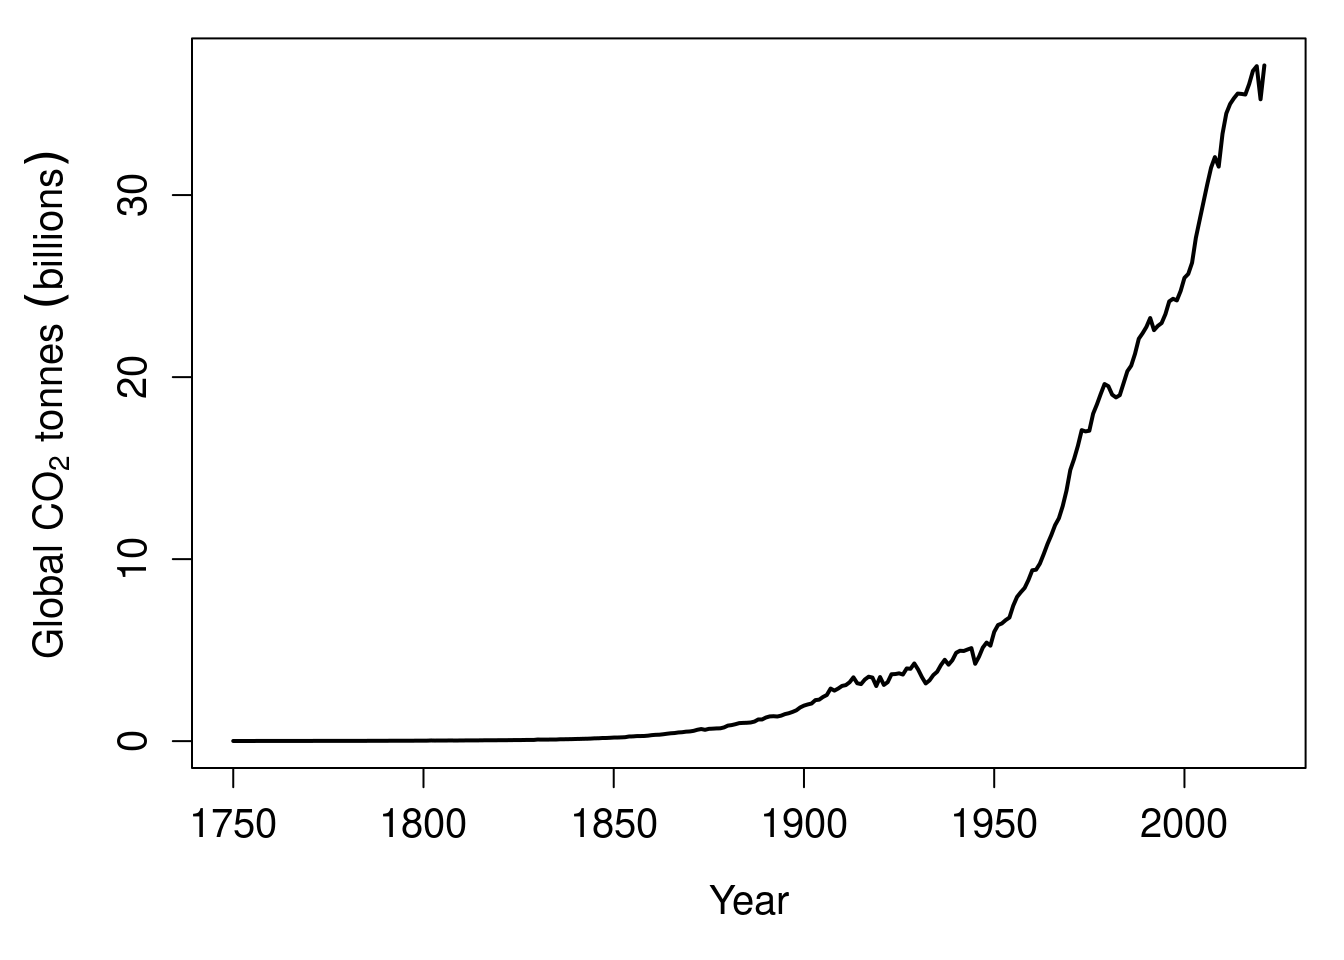
\includegraphics[width=1\linewidth]{bookdown-demo_files/figure-latex/unnamed-chunk-2-1} \caption{Global carbon dioxide emissions from 1750-2021.}\label{fig:unnamed-chunk-2}
\end{figure}

We can see from Figure 1.1 that global CO\(_{2}\) emissions go up exponentially over time, but this exponential relationship means that the y-axis has to cover a large range of values.
This makes it difficult to see what is actually happening in the first 100 years.
Are CO\(_{2}\) emissions increasing from 1750-1850, or do they stay about the same?
If instead of plotting billions of tonnes of CO\(_{2}\) on the y-axis, we plotted the logarithm of these values, then the pattern in the first 100 years becomes a bit more clear (Figure 1.2).

\begin{figure}
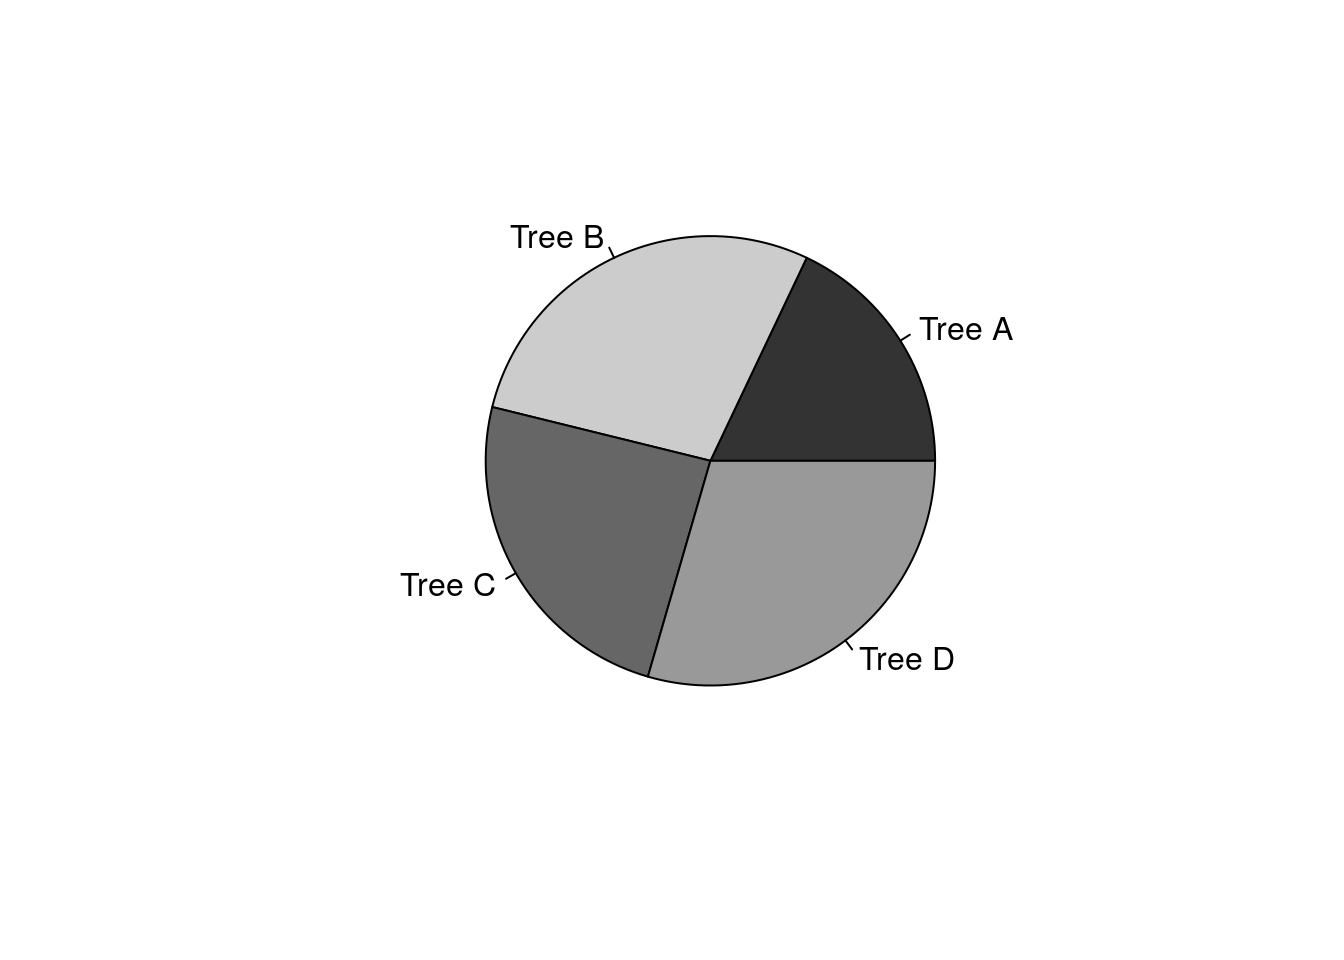
\includegraphics[width=1\linewidth]{bookdown-demo_files/figure-latex/unnamed-chunk-3-1} \caption{Natural logarithm of global carbon dioxide emissions from 1750-2021.}\label{fig:unnamed-chunk-3}
\end{figure}

It appears from the logged data in Figure 1.2 that global CO\(_{2}\) emissions were indeed increasing from 1750-1850.
Note that Figure 1.2 presents the \emph{natural logarithm} of CO\(_{2}\) emissions on the y-axis.
The natural logarithm uses Euler's number, \(e \approx 2.718282\), as a base.
Euler's number \(e\) is an irrational number (like \(\pi\)), which corresponds to the intrinsic rate of increase of a population's size in ecology \citep{Gotelli2001}, or, in banking, interest compounded continually (like \(\pi\), \(e\) actually shows up in a lot of different places throughout science and mathematics).
We probably could have just as easily used 10 as a base, but \(e\) is usually the default base to use in science (bases 10 or 2 are also often used).
Note that we can convert back to the non-logged scale by raising numbers to the power of \(e\).
For example, \(e^{-4} \approx 0.018\), \(e^{-2} \approx 0.135\), \(e^{0} = 1\), and \(e^{2} = 7.390\).

\hypertarget{order-of-operations}{%
\section{Order of operations}\label{order-of-operations}}

Every once in a while, a maths problem like the one below seems to go viral online,

\[x = 8 \div 2\left(2+2\right).\]

Depending on the order in which calculations are made, some people will conclude that \(x = 16\), while others conclude that \(x = 1\) \citep{Chernoff2022}.
The confusion is not caused by the above calculation being difficult, but by peoples' differences in interpreting the rules for what order calculations should be carried out.
If we first divide 8/2 to get 4, then multiply by (2 + 2), we get 16.
If we first multiply 2 by (2 + 2) to get 8, then divide, we get 1.
The truth is that even if there is a `right' answer here \citep{Chernoff2022}, the equation could be written more clearly.
We might, for example, rewrite the above to more clearly express the intended order of operations,

\[x = \frac{8}{2}\left(2 + 2\right) = 16.\]

We could write it a different way to express a different intended order of operations,

\[x = \frac{8}{2(2+2)} = 1.\]

The key point is that the order in which operations are calculated matters, so it is important to write equations clearly, and to know the order of operations to calculate an answer correctly.
By convention, there are some rules for the order in which calculations should proceed.

\begin{enumerate}
\def\labelenumi{\arabic{enumi}.}
\tightlist
\item
  Anything within parentheses should always be calculated first.
\item
  Exponents and radicals should be applied second
\item
  Multiplication and division should be applied third
\item
  Addition and subtraction should be done last
\end{enumerate}

These conventions are not really rooted in anything fundamental about numbers or operations (i.e., we made these rules up), but there is a logic to them.
First, parentheses are a useful tool for being unequivocal about the order of operations.
We could, for example, always be completely clear about the order to calculate by writing something like \((8/2) \times (2+2)\) or \(8 / (2(2 + 2))\), although this can get a bit messy.
Second, rules 2-4 are ordered by the magnitude of operation effects; for example, exponents have a bigger effect than multiplication, which has a bigger effect than addition.
In general, however, these are just standard conventions that need to be known for reading and writing mathematical expressions.
In this module, you will not see something ambiguous like \(x = 8 \div 2\left(2+2\right)\), but you should be able to correctly calculate something like this,

\[x = 3^{2} + 2\left(1 + 3\right)^{2} - 6 \times 0.\]

First, remember that parentheses come first, so we can rewrite the above,

\[x = 3^{2} + 2\left(4\right)^{2} - 6 \times 0.\]

Exponents come next, so we can calculate those,

\[x = 9 + 2\left(16\right) - 6 \times 0.\]

Next comes multiplication and division,

\[x = 9 + 32 -  0.\]

Lastly, we calculate addition and subtraction,

\[x = 41.\]

In this module, you will very rarely need to calculate something with this many different steps.
But you will often need to calculate equations like the one below,

\[x = 20 + 1.96 \times 2.1.\]

It is important to remember to multiply \(1.96 \times 2.1\) \emph{before} adding 20.
Getting the order of operations wrong will usually result in the calculation being completely off.

One last note is that when operations are above or below a fraction, or below a radical, then parentheses are implied.
For example, we might have something like the fraction below,

\[x = \frac{2^{2} + 1}{3^{2} +2}.\]

Although rules 2-4 still apply, it is implied that there are parentheses around both the top (numerator) and bottom (denominator), so you can always read the above equation like this,

\[x = \frac{\left(2^{2} + 1\right)}{\left(3^{2} + 2\right)} = \frac{\left(4 + 1\right)}{\left(9 + 2\right)} = \frac{5}{11}.\]

Similarly, anything under the \(\sqrt{}\) can be interpreted as being within parentheses.
For example,

\[x = \sqrt{3 + 4^{2}} = \sqrt{\left(3 + 4^{2} \right)} \approx 4.47.\]

This can take some getting used to, but with practice, it will become second nature to read equations with the correct order of operations.

\hypertarget{Chapter_2}{%
\chapter{Data organisation}\label{Chapter_2}}

In the field or the lab, data collection can be messy.
Often data need to be recorded with a pencil and paper, and in a format that is easiest for writing in adverse weather or a tightly controlled laboratory.
Sometimes data from a particular sample, such as a bird nest (Figure 2.1), cannot all be collected in one place.

\begin{figure}
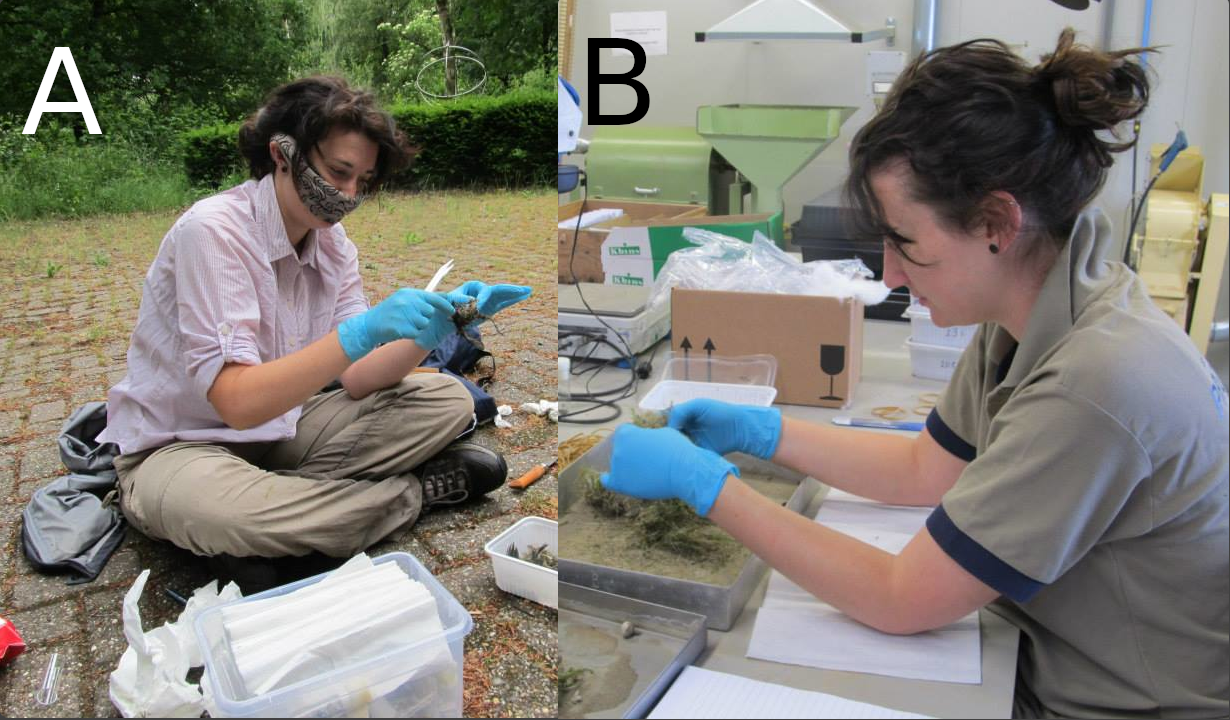
\includegraphics[width=1\linewidth]{img/becky_field} \caption{Dr Becky Boulton collects data from nest boxes in the field (A), then processes nest material in the lab (B).}\label{fig:unnamed-chunk-4}
\end{figure}

Data are sometimes missing due to circumstances outwith the researcher's control, and data are usually not collected in a format that is immediately ready for statistical analysis (e.g., Figure 2.2).
Consequently, we often need to reorganise data from a lab or field book to a spreadsheet on the computer.

\begin{figure}
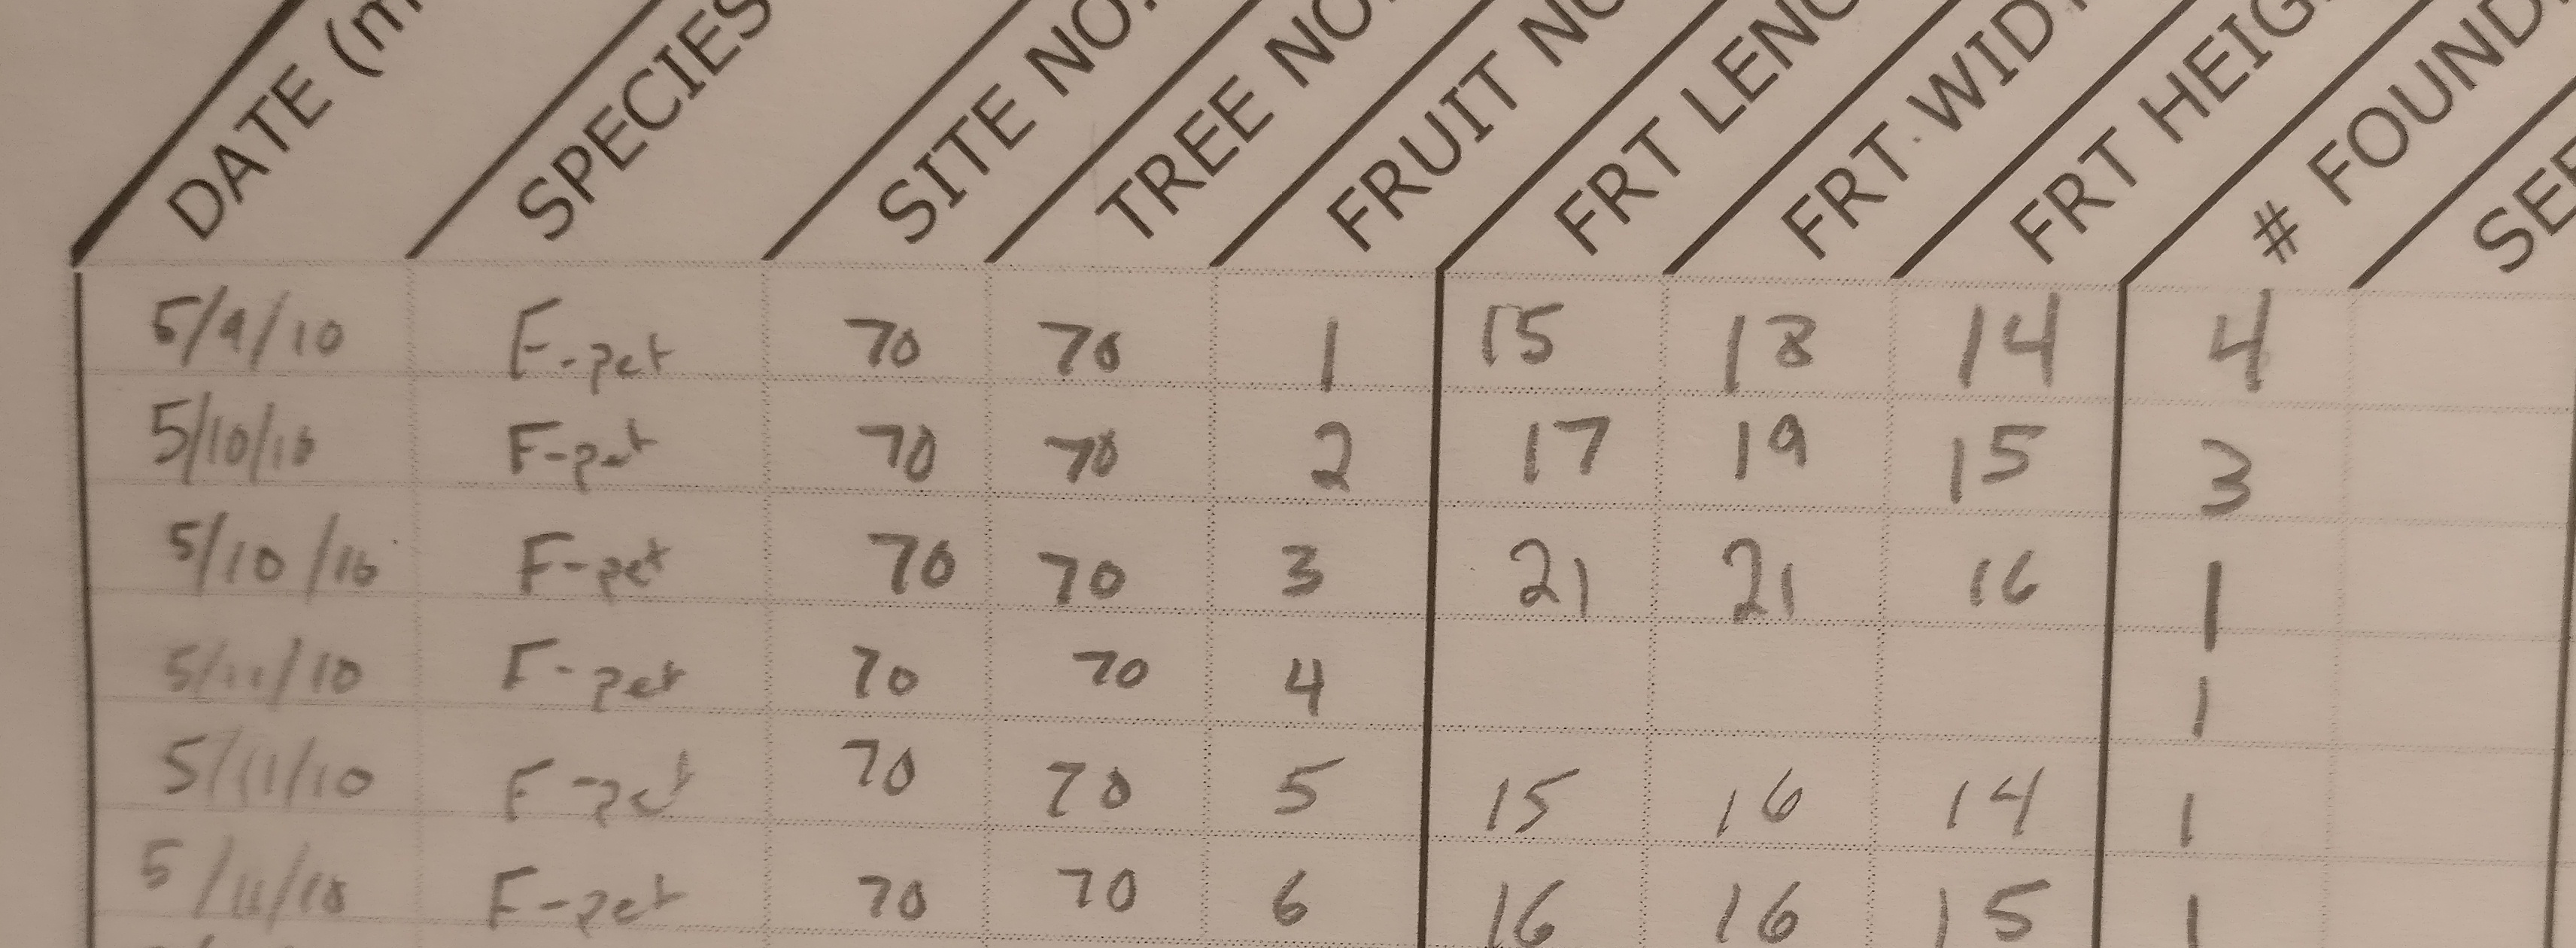
\includegraphics[width=1\linewidth]{img/handwritten_data} \caption{A portion of a lab notebook used to record measurements of fig fruits from different trees in Baja, Mexico, in 2010.}\label{fig:unnamed-chunk-5}
\end{figure}

Fortunately, there are some generally agreed upon guidelines for formatting data for statistical analysis.
This chapter introduces the tidy format \citep{Wickham2014}, which can be used for structuring data files for statistical software.
This chapter will provide an example of how to put data into a tidy format, and how to save a dataset into a file that can be read and used in statistical software such as Jamovi or R.

\hypertarget{tidy-data}{%
\section{Tidy data}\label{tidy-data}}

After data are collected, they need to be stored digitally (i.e., in a computer file, such as a spreadsheet).
This should happen as soon as possible so that back up copies of the data can be made.
Nevertheless, retaining field and lab notes as a record of the originally collected data is also a good idea.
Sometimes it is necessary to return to these notes, even years after data collection.
Often we will want to double-check to make sure that we copied a value or observation correctly from handwritten notes to a spreadsheet.
Note that sometimes data can be input directly into a spreadsheet or mobile application, bypassing handwritten notes altogether, but it is usually helpful to have a physical copy of collected data.

Most biological and environmental scientists store data digitally in the form of a spreadsheet.
Spreadsheets enable data input, manipulation, and calculation in a highly flexible way.
Most spreadsheet programs even have some capacity for data visualisation and statistical analysis.
For the purposes of statistical analysis, spreadsheets are probably most often used for inputting data in a way that can be used by more powerful statistical software.
Commonly used spreadsheet programs are MS Excel, Google Sheets, LibreOffice Calc.
The interface and functions of these programs are very similar, nearly identical for most purposes.
They can all open and save the same file types (e.g., XLSX, ODS, CSV), and they all have the same overall look, feel, and functionality for data input, so the program used is mostly a matter of personal preference.
In this text, we will use LibreOffice because it is completely free and open source, and easily available to \href{https://www.libreoffice.org/download/download-libreoffice/}{download} at \url{http://libreoffice.org}.
Excel and \href{https://docs.google.com/spreadsheets}{Google Sheets} are also completely fine to use.

\begin{figure}
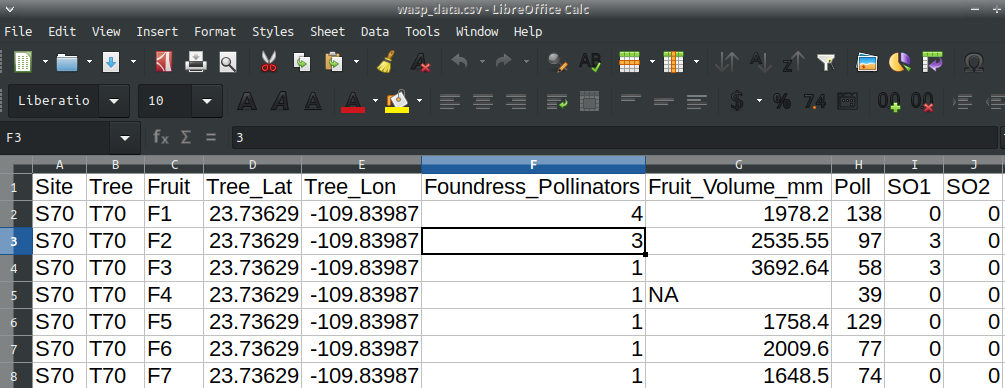
\includegraphics[width=1\linewidth]{img/wasp_data_spreadsheet} \caption{A LibreOffice spreadsheet showing data from fig fruits collected in 2010. Each row is a unique sample (fruit), and columns record properties of the fruit.}\label{fig:unnamed-chunk-6}
\end{figure}

Spreadsheets are separated into individual rectangular cells, which are identified by a specific column and row (Figure 2.3).
Columns are indicated by letters, and rows are indicated by numbers.
We can refer to a specific cell by its letter and number combination.
For example, the active cell in Figure 2.3 is F3, which has a value of `3' indicating the value recorded in that specific measurement (in this case, foundress pollinators in the fig fruit).
We will look more at how to interact with the spreadsheet in the \protect\hyperlink{Chapter_3}{Chapter 3} lab practical, but for now we will focus on how the data are organised.

There are a lot of potential ways that data could be organised in a spreadsheet.
For good statistical analysis, there are a few principles that are helpful to follow.
Whenever we collect data, we record observations about different units.
For example, we might make one or more measurements on a tree, a patch of land, or a sample of soil.
In this case, trees, land patches, or soil samples are our units of \textbf{observation}.
Each attribute of a unit that we are measuring is a \textbf{variable}.
These variables might include tree heights and leaf lengths, forest cover in a patch of land, or carbon and nitrogen content of a soil sample.
Tidy datasets that can be used in statistical analysis programs are defined by three characteristics \citep{Wickham2014}.

\begin{enumerate}
\def\labelenumi{\arabic{enumi}.}
\tightlist
\item
  Each variable gets its own column.
\item
  Each observation gets its own row.
\item
  Different units of observation require different data files.
\end{enumerate}

If, for example, we were to measure the heights and leaf lengths for 4 trees, we might organise the data as in Table 2.1.

\begin{longtable}[]{@{}llll@{}}
\caption{Hypothetical tidy dataset in which each column of data is a variable and each row of data is an observational unit (tree).}\tabularnewline
\toprule
Tree & Species & Height (m) & Leaf length (cm) \\
\midrule
\endfirsthead
\toprule
Tree & Species & Height (m) & Leaf length (cm) \\
\midrule
\endhead
1 & Oak & 20.3 & 8.1 \\
2 & Oak & 25.4 & 9.4 \\
3 & Maple & 18.2 & 12.5 \\
4 & Maple & 16.7 & 11.3 \\
\bottomrule
\end{longtable}

By convention \citep{Wickham2014}, variables tend to be in the left-most columns if they are known in advance or fixed in some way by the data collection or experiment (e.g., tree number or species in Table 2.1).
In contrast, variables that are actually measured tend to be in the right-most columns (e.g., tree height or leaf length).
This is more for readability of the data; statistical software such as Jamovi will not care about the order of data columns.

\hypertarget{data-files}{%
\section{Data files}\label{data-files}}

Data can be saved using many different file types.
File type is typically indicated by an extension following the name of a file and a full stop.
For example, ``photo.png'' would indicate a PNG image file named ``photo''.
A peer-reviewed journal article might be saved as a PDF, e.g., ``Wickham2014.pdf''.
A file's type affects what programs can be used to open it.
One relevant distinction to make is between text files and binary files.

\textbf{Text files} are generally very simple.
They only allow information to be stored as plain text; no colour, bold, italic, or anything else is encoded.
All of the information is just made up of characters on one or more lines.
This sounds so simple as to be almost obsolete; what is the point of not allowing anything besides plain text?
The point is that text files are generally much more secure for long-term storage.
The plain text format makes data easier to recover if a file is corrupted, readable by a wider range of software, and more amenable to version control (\href{https://bradduthie.github.io/version_control/vc_notes.html}{version control} is a tool that essentially saves the whole history of folder, and potentially different versions of it in parallel; it is not necessary for introductory statistics, but is often critical for big collaborative projects).
There are many types of text files with extensions such as TXT, CSV, HTML, R, CPP, or MD.
For data storage, we will use comma separated value (CSV) files.
As the name implies, CSV files include plain text separated by commas.
Each line of the CSV file is a new row, and commas separate information into columns.
These CSV files can be opened in any text editor, but are also recognised by nearly all spreadsheet programs and statistical software.
The data shown in Figure 2.3 are from a CSV file called ``wasp\_data.csv''.
Figure 2.4 shows the same data when opened with a text editor.

\begin{figure}
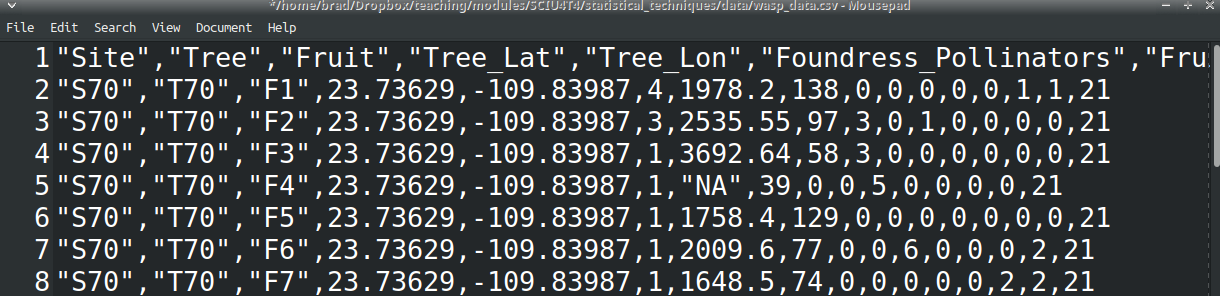
\includegraphics[width=1\linewidth]{img/wasp_data_csv} \caption{A plain text comma-separated value (CSV) file showing data from fig fruits collected in 2010. Each line is a unique row and sample (fruit), and commas separate the data into columns in which the properties of fruit are recorded. The file has been opened in a program called 'Mousepad', but it could also be opened in any text editor such as gedit, Notepad, vim, or emacs. It could also be opened in spreadsheet programs such as LibreOffice Calc, MS Excel, or Google Sheets, or in any number of statistical programs.}\label{fig:unnamed-chunk-7}
\end{figure}

The data shown in Figure 2.4 are not easy to read or work with, but the format is highly effective for storage because all of the information is in plain text.
The information will therefore always look \emph{exactly} the same, and can be easily recovered by any text editor, even after years pass and old software inevitably becomes obsolete.

\textbf{Binary files} are different from text files and contain information besides just plain text.
This information could include formatted text (e.g., bold, italic), images, sound, or video (basically, anything that can be stored in a file).
The advantages of being able to store this kind of information are obvious, but the downside is that the information needs to be interpreted in a specific way, usually using a specific program.
Examples of binary files include those with extensions such as DOC, XLS, PNG, GIF, MP3, or PPT.
Some file types such as DOCX are not technically binary files, but a collection of zipped files (which, in the case of DOCX, include plain text files).
Overall, the important point is that saving data in a text file format such as CSV is generally more secure.

\hypertarget{managing-data-files}{%
\section{Managing data files}\label{managing-data-files}}

Managing data files (or any files) effectively requires some understanding of how files are organised on a computer or cloud storage.
In mobile phone applications, file organisation is often hidden, so it is not obvious where a file actually goes when it is saved on a device.
Many people find files in these applications using a search function.
The ability to search for files like this, or at least the tendency to do so regularly, is actually a relatively new phenomenon.
And it is an approach to file organisation that does not work quite as well on non-mobile devices (i.e., anything that is not a phone or tablet), especially for big projects.
On laptop and desktop computers, it is really important to know \emph{where} files are being saved, and to ideally have an organisational system that makes it easy to find specific files without having to use a search tool.

On a computer, files are stored in a series of nested folders.
You can think of the storage space on a computer, cloud, or network drive, as a big box.
The big box can contain other smaller boxes (folders, in this analogy), or it can contain items that you need (files, in this analogy).
Figure 2.5 shows the general idea.
On this computer, there is a folder called `brad', which has inside it 5 other folders (Figure 2.5A).
Each of the 5 inner folders is used to store more folders and files for a specific module from 2006.
Clicking on the `Biostatistics' folder leads to the sub-folders inside it, and to files saved specifically for a biostatistics module (e.g., homework assignments, lecture notes, and an exam review document).
Files on a computer therefore have a location that we can find using a particular \textbf{path}.
We can write the path name using slashes to indicate nested folders.
For example, the file `HW9.scx' in Figure 2.5B would have the path name `/home/brad/Spring\_2006/Biostatistics/HW9.scx'.
Each folder is contained within slashes, and the file name itself is after the last slash.

\begin{figure}
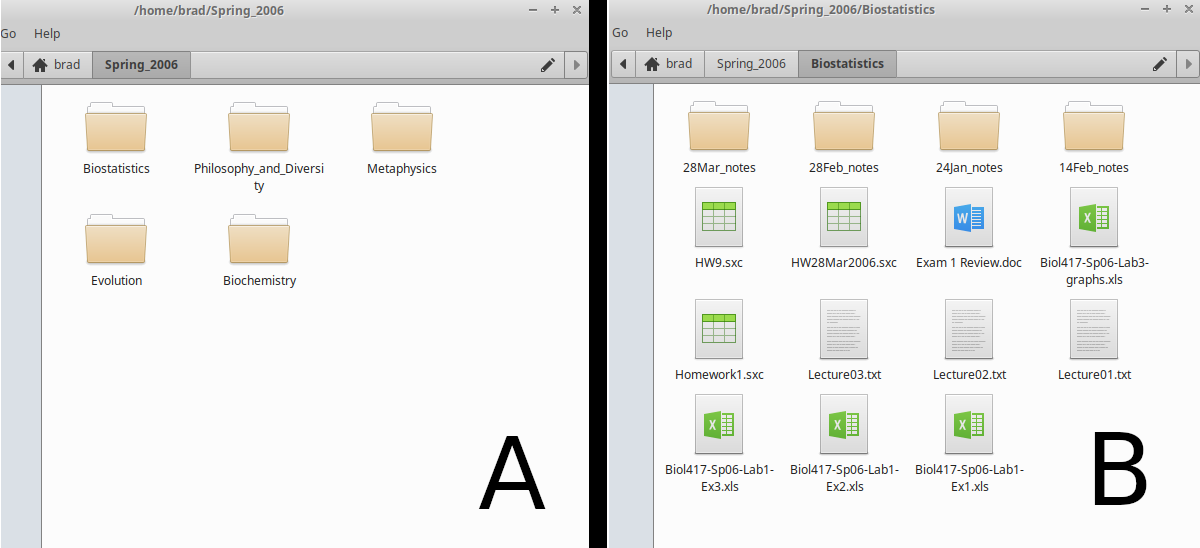
\includegraphics[width=1\linewidth]{img/directory_eg} \caption{File directory of a computer showing (A) the file organisation of modules taken during spring 2006. Within one folder (B), there are multiple sub-folders and files associated with a biostatistics module.}\label{fig:unnamed-chunk-8}
\end{figure}

These path names might look slightly different depending on the computer operating system that you are using.
But the general idea of files nested within folders is the same.
Figure 2.6 shows the same folder `Spring\_2006' saved in a different location, on OneDrive.

\begin{figure}
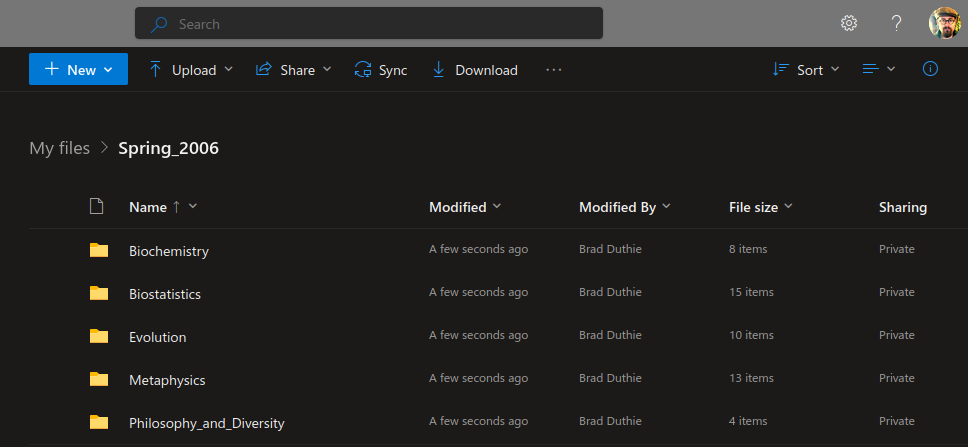
\includegraphics[width=1\linewidth]{img/OneDrive} \caption{OneDrive file directory showing the file organisation of modules taken during spring 2006.}\label{fig:unnamed-chunk-9}
\end{figure}

Windows has the same general file organisation (Figure 2.7).
Path names for storing files on the hard drive of a Windows computer look something like ``C:\textbackslash Users\textbackslash MyName\textbackslash Desktop\textbackslash Spring\_2006\textbackslash Biostatistics\textbackslash HW9.scx''.
The `C:\textbackslash{}' is the root directory of the hard drive; it is called `C' for historical reasons (`A:\textbackslash{}' and `B:\textbackslash{}' used to be for floppy disks; the `A:\textbackslash{}' floppy disks had about 1.44 MB of storage, and `B:\textbackslash{}' had even less, so these are basically obsolete).

\begin{figure}
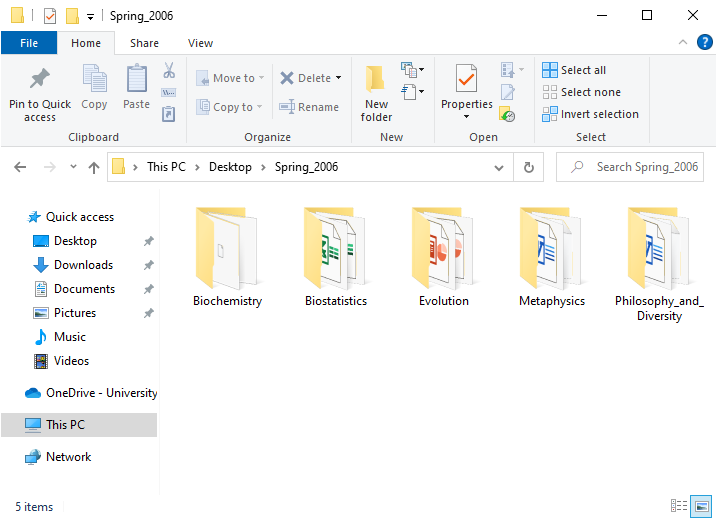
\includegraphics[width=1\linewidth]{img/directory_windows} \caption{Windows file directory showing the file organisation of modules taken during spring 2006. In this case, the 'Spring\_2006' folder is located on the desktop; the path to the folder is visible in the toolbar above the folders.}\label{fig:unnamed-chunk-10}
\end{figure}

The details are not as important as the idea of organising files in a logical way that allows you to know roughly where to find important files on a computer or cloud drive.
It is usually a good idea to give every unique project or subject (e.g., a university module, a student group, holiday plans, health records) its own folder.
This makes it much easier to find related files such as datasets, lecture notes, or assignments when necessary.
It is usually possible to right click somewhere in a directory to create a new folder.
In Figure 2.7, there is even a `New folder' button in the toolbar with a yellow folder icon above it.
It takes some time to organise files this way, and to get used to saving files in specific locations, but it is well worth it in the long-term.

\hypertarget{Chapter_3}{%
\chapter{Practical: Preparing data}\label{Chapter_3}}

In this practical, we will use a spreadsheet to organise datasets following the tidy approach explained in \protect\hyperlink{Chapter_2}{Chapter 2}, then save these datasets as CSV files to be opened in Jamovi statistical software.
The data organisation in this lab can be completed using \href{https://www.libreoffice.org/discover/calc/}{LibreOffice Calc}, MS Excel, or \href{https://docs.google.com/spreadsheets/}{Google Sheets}.
In the computer lab, MS Excel is probably the easiest program to use, either through AppsAnywhere or within a browser.
The screenshots below will mostly be of LibreOffice Calc, but the instructions provided will work on any of the three aforementioned spreadsheet programs.
You can download a PDF of this practical \href{https://bradduthie.github.io/SCIU4T4/chapters/chapter_3.pdf}{here}, or a DOCX of just the questions \href{https://bradduthie.github.io/SCIU4T4/practical_answers/Week1.docx}{here}.

There are 4 data exercises in this practical.
All of these exercises will focus on organising data into a tidy format.
Being able to do this will be essential for later practicals and assessments, and for future modules (especially fourth year dissertation work).
Exercise 1 uses handwritten field data that need to be entered into a spreadsheet in a tidy format.
These data include information shown in Figure 2.2, plus tallies of seed counts.
The goal is to get all of this information into a tidy format and save it as a CSV file.
Exercise 2 presents some data on the number of eggs produced by five different fig wasp species (more on these in \protect\hyperlink{Chapter_8}{Chapter 8}).
The data are in an untidy format, so the goal is to reorganise them and save them as a tidy CSV file.
Exercise 3 presents counts of the same five fig wasp species as in Exercise 2, which need to be reorganised in a tidy format.
Exercise 4 presents data that are even more messy.
These are morphological measurements of the same five species of wasps, including lengths and widths of wasp heads, thoraxes, and abdomens.
The goal in this exercise is to tidy the data, then estimate total wasp volume from the morphological measurements using mathematical formulas, keeping in mind the order of operations from \protect\hyperlink{Chapter_1}{Chapter 1}.

\hypertarget{exercise-1-transferring-data-to-a-spreadsheet}{%
\section{Exercise 1: Transferring data to a spreadsheet}\label{exercise-1-transferring-data-to-a-spreadsheet}}

Exercise 1 focuses on data collected from the fruits of fig trees collected from Baja, Mexico in 2010 \citep{Duthie2015b, Duthie2016}.
Due to the nature of the work, the data needed to be recorded in notebooks and collected in two different locations.
The first location was the field, where data were collected identifying tree locations and fruit dimensions.
Baja is hot and sunny; fruit measurements were made with a ruler and recorded in a field notebook.
These measurements are shown in Figure 2.2, which is reproduced again in Figure 3.1.

\begin{figure}
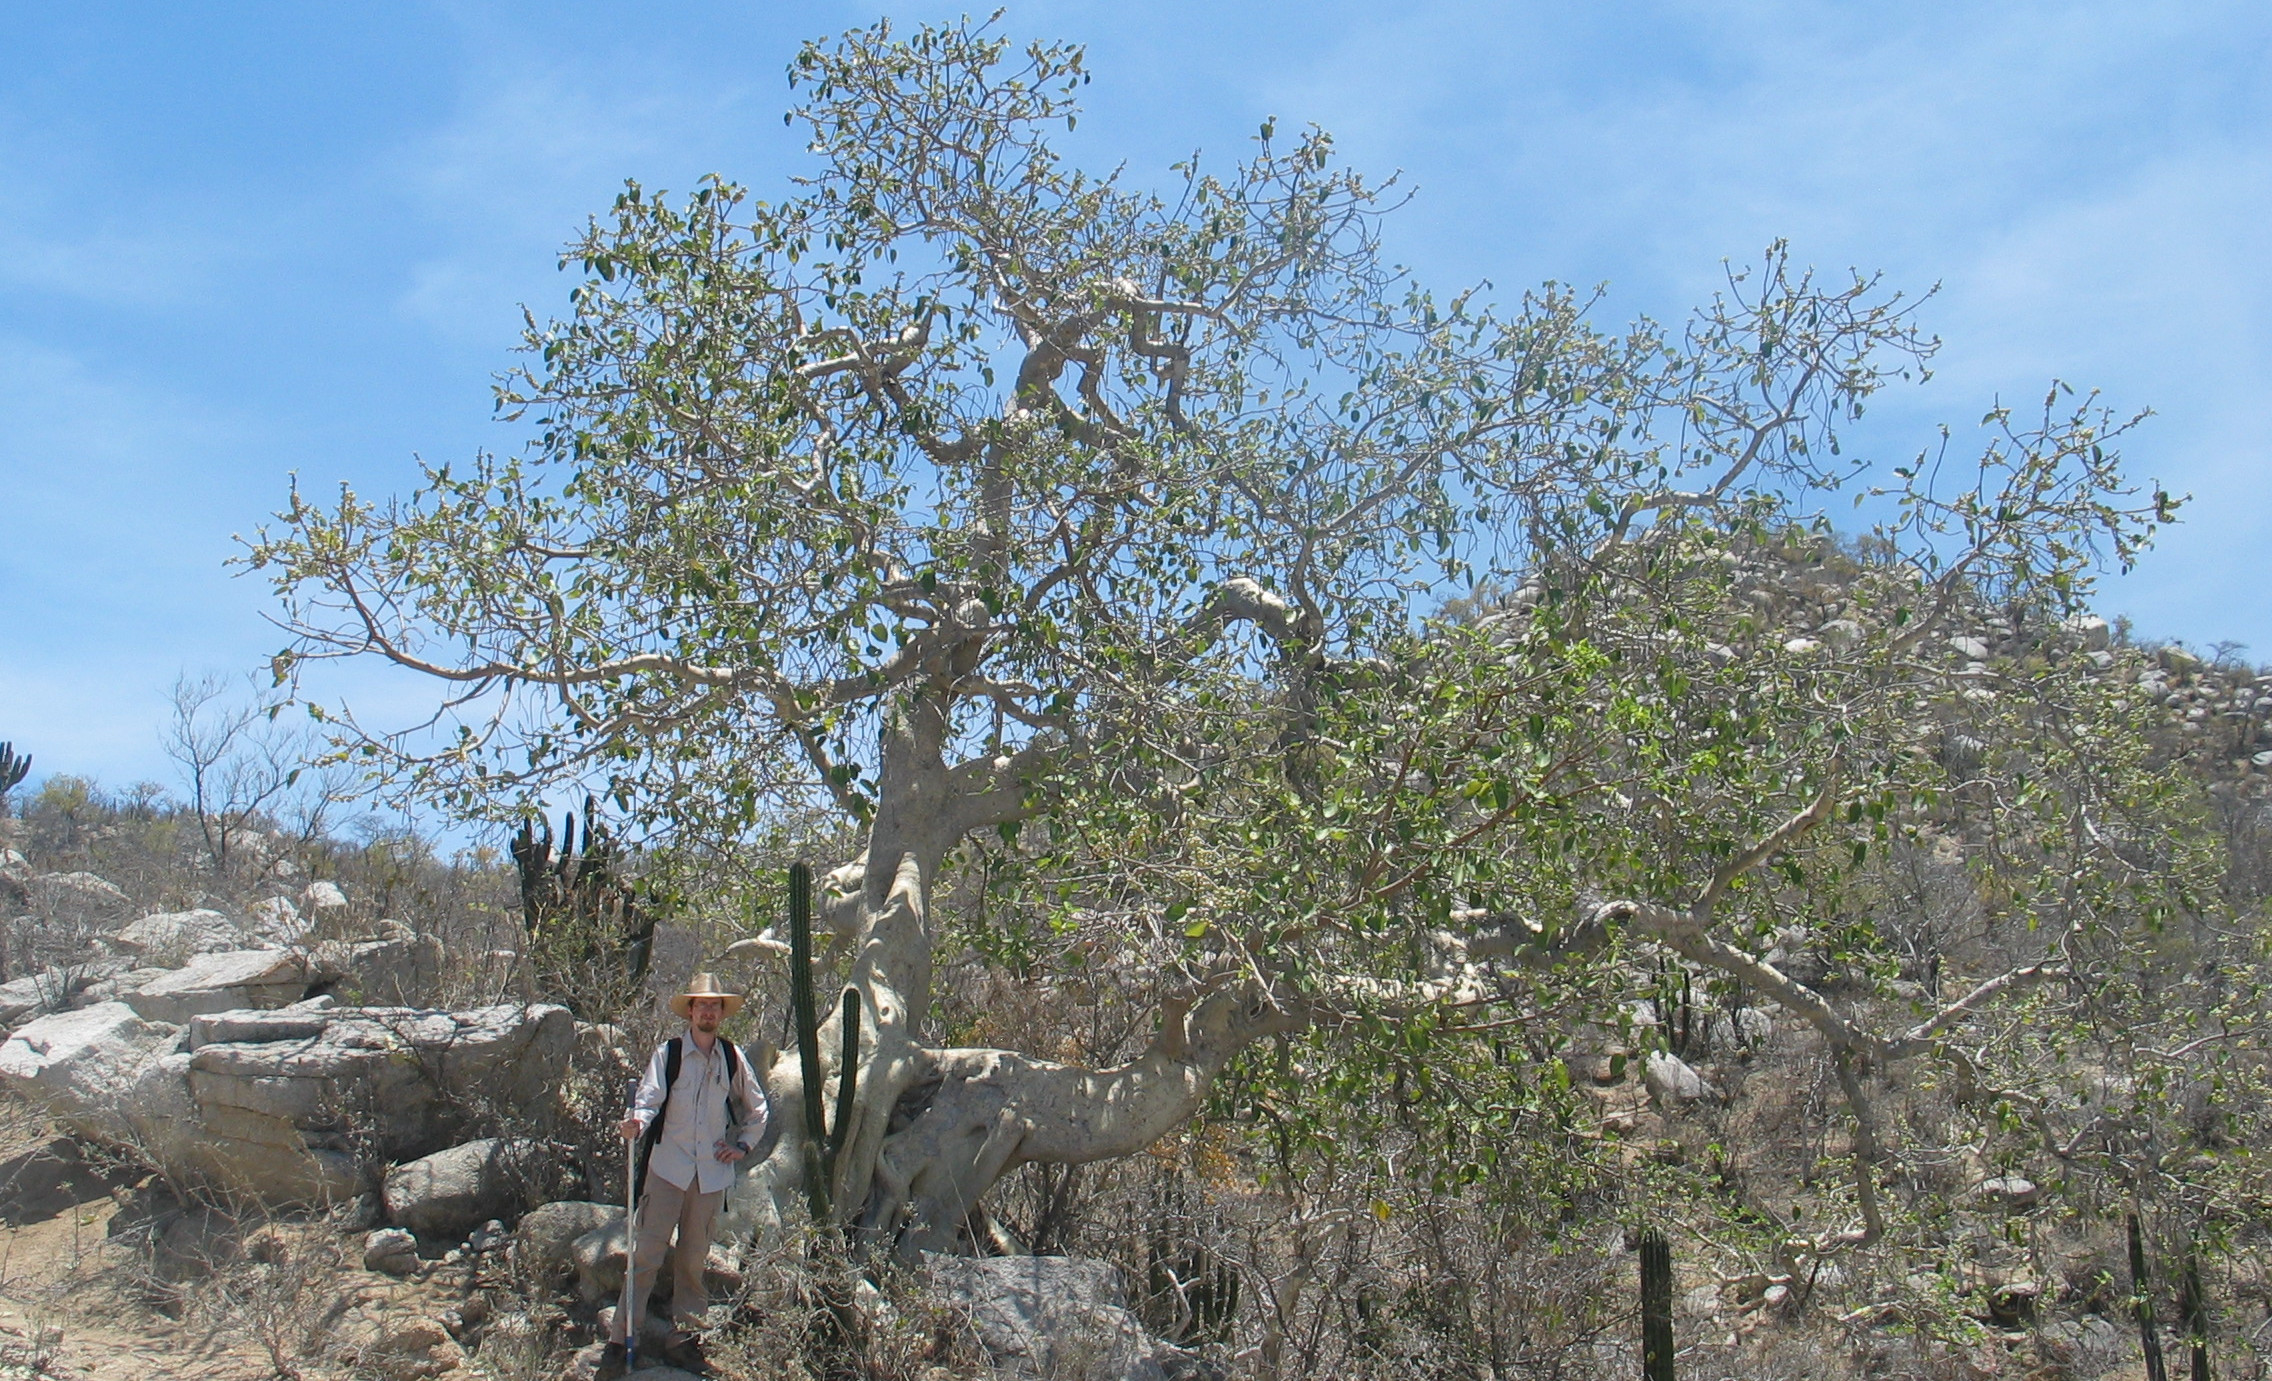
\includegraphics[width=1\linewidth]{img/Ficus_petiolaris} \caption{A fully grown Sonoran Desert Rock Fig in the desert of Baja, Mexico.}\label{fig:unnamed-chunk-11}
\end{figure}

The second location was in a lab in Iowa, USA.
Fruits were dried and shipped to Iowa State University so that seeds could be counted under a microscope.
Counts were originally recorded as tallies in a lab notebook (Figure 3.2).
The goal of Exercise 1 is to get all of this information into a single tidy spreadsheet.

\begin{figure}
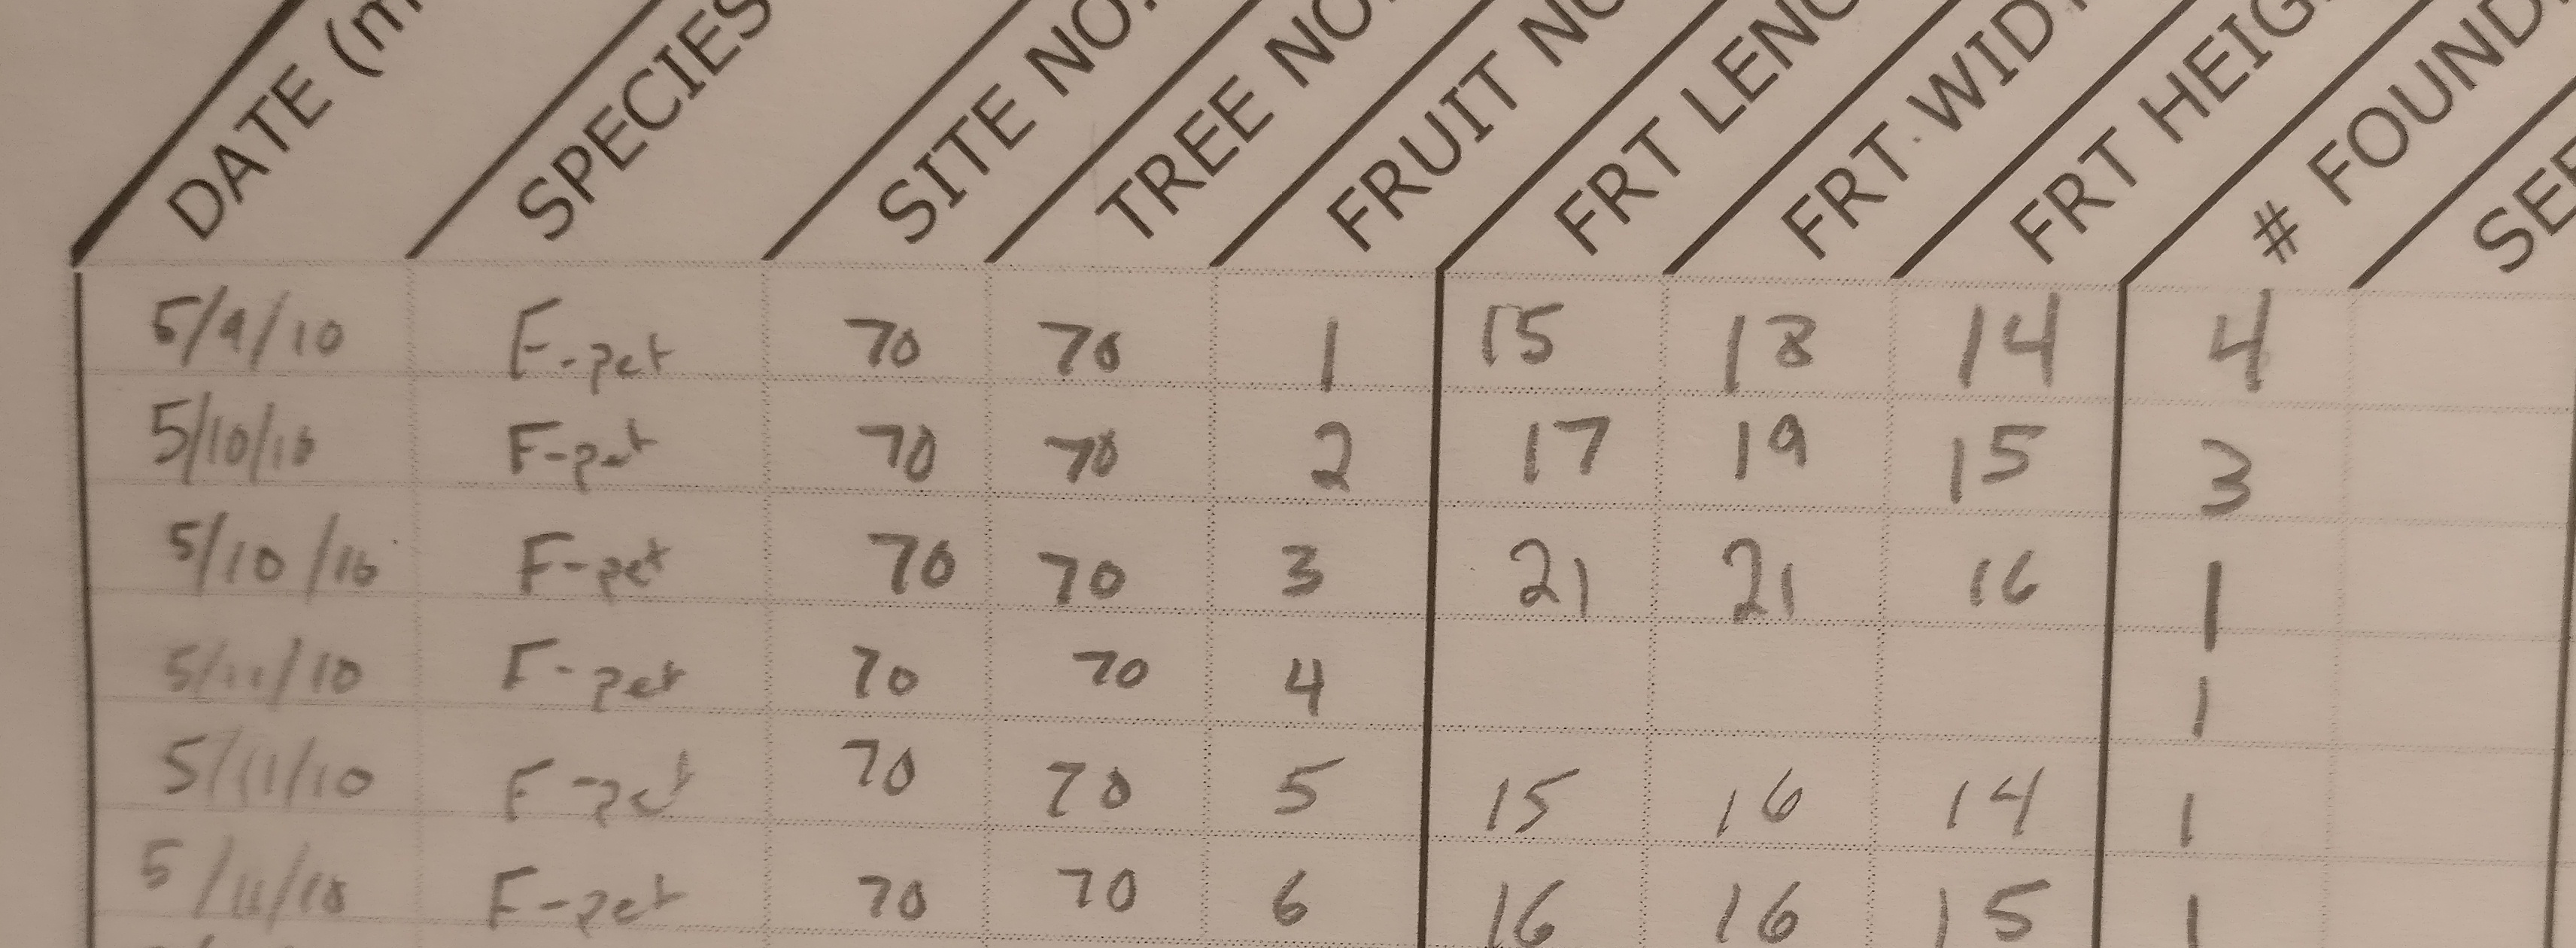
\includegraphics[width=1\linewidth]{img/handwritten_data} \caption{A portion of a lab notebook used to record measurements of fig fruits from different trees in 2010.}\label{fig:unnamed-chunk-12}
\end{figure}

The best place to start is with an empty spreadsheet, so open a new one in LibreOffice Calc, MS Excel, or Google Sheets.
Remember that each row will be a unique observation; in this case, a unique fig fruit from which measurements were recorded.
Each column will be a variable of that observation.
Fortunately, the data in Figure 3.2 are already looking quite tidy.
The information here can be put into the spreadsheet mostly as written in the notebook.
But there are a few points to keep in mind:

\begin{enumerate}
\def\labelenumi{\arabic{enumi}.}
\tightlist
\item
  It is important to start in column A and row 1; do not leave any empty rows or columns because when we get to the statistical analysis in Jamovi, Jamovi will assume that these empty rows and columns signify missing data.
\item
  There is no need to include any formatting (e.g., bold, underline, colour) because it will not be saved in the CSV or recognised by Jamovi.
\item
  Missing information, such as the empty boxes for the fruit dimensions in row 4 in the notebook (Figure 3.2) should be indicated with an `\texttt{NA}' (capital letters, but without the quotes). This will let Jamovi know that these data are missing.
\item
  The date is written in an American style of month-day-year, which might get confusing. It might be better to have separate columns for year, month, and day, and to write out the full year (2010).
\end{enumerate}

The column names in Figure 3.2 are (1) Date, (2) Species, (3) Site number, (4) Tree number, (5) Fruit length in mm, (6) Fruit width in mm, and (7) Fruit height in mm.
All of the species are \emph{Ficus petiolaris}, which is abbreviated to ``F-pet'' in the field notebook.
How you choose to write some of this information down is up to you (e.g., the date format, capitalisation of column names), but when finished, the spreadsheet should be organised like the one in Figure 3.3.

\begin{figure}
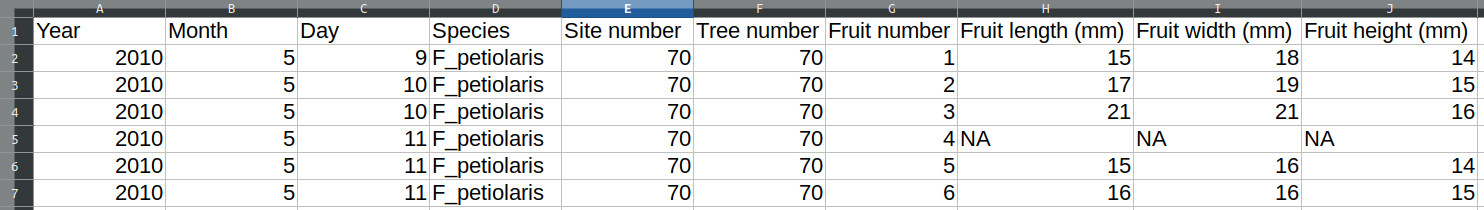
\includegraphics[width=1\linewidth]{img/Ch1_Ex1a} \caption{A spreadsheet with data organised in a tidy format and nearly ready for analysis.}\label{fig:unnamed-chunk-13}
\end{figure}

This leaves us with the data that had to be collected later in the lab.
Small seeds needed to be meticulously separated from other material in the fig fruit, then tallied under a microscope.
Tallies from this notebook are shown in Figures 3.4 and 3.5.

\begin{figure}
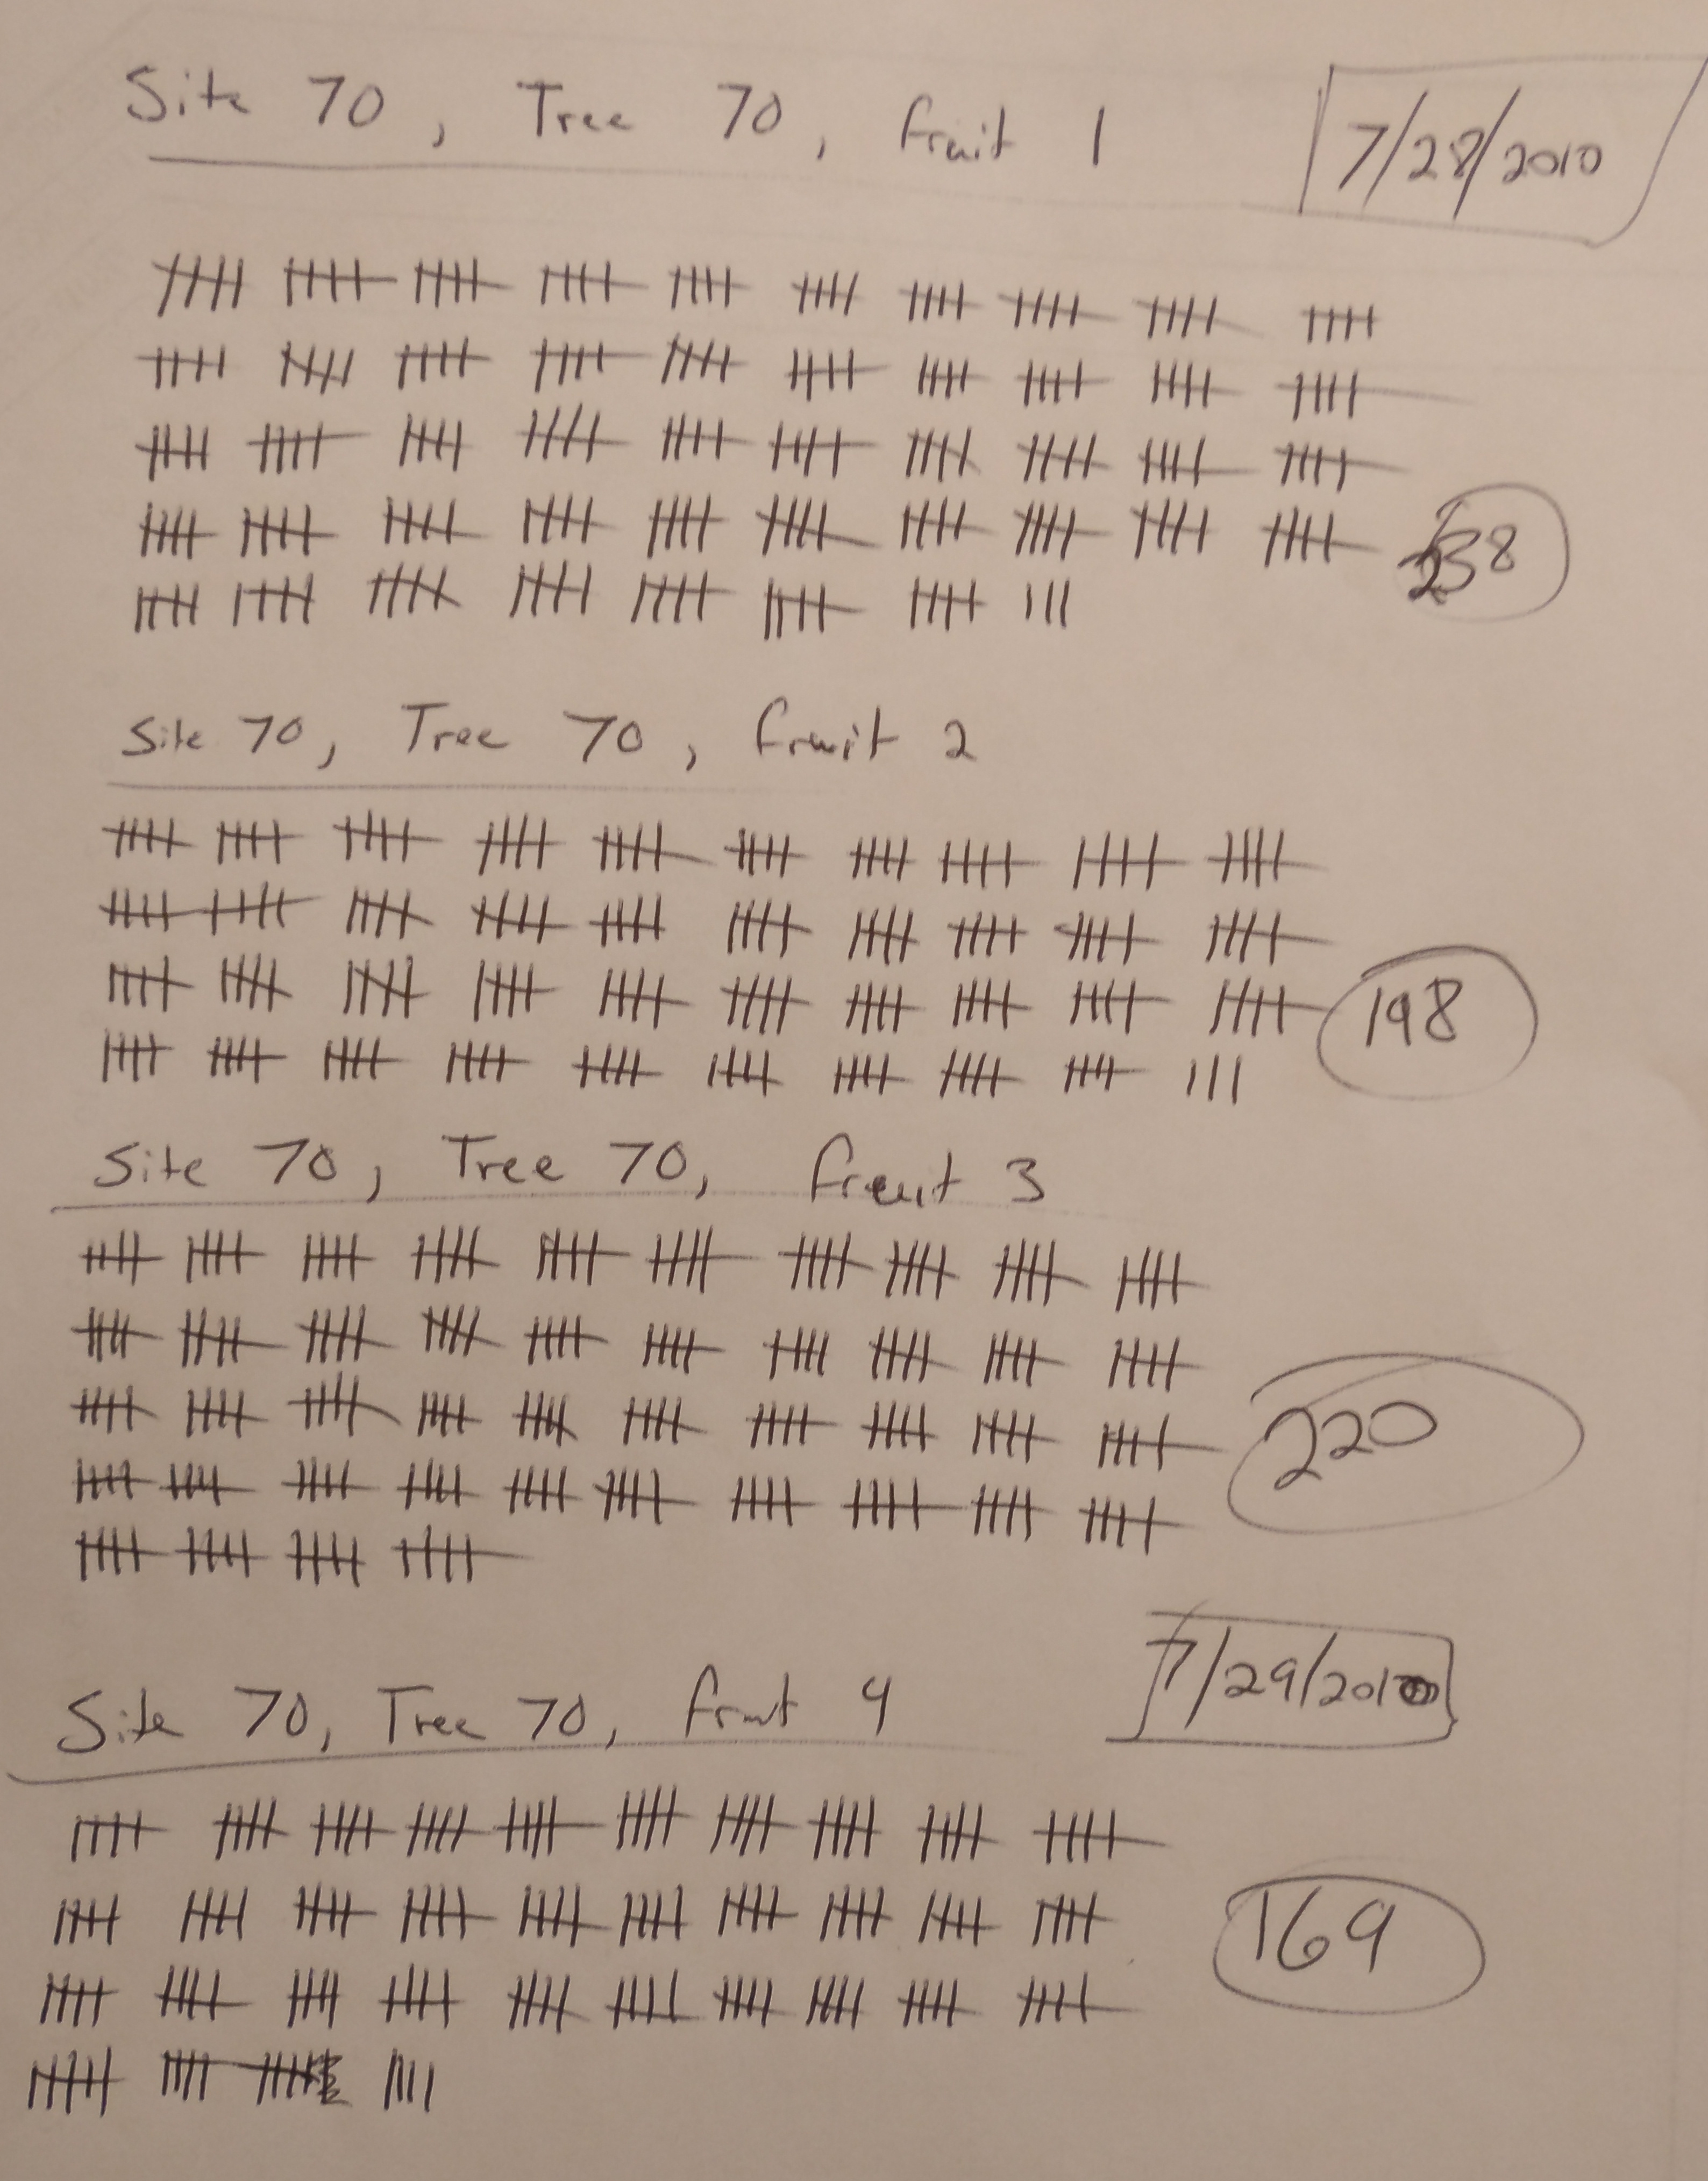
\includegraphics[width=1\linewidth]{img/Ch1_Ex1_seeds1} \caption{Tallies of seed counts collected from 4 fig fruits in Baja, Mexico in 2010.}\label{fig:unnamed-chunk-14}
\end{figure}

\begin{figure}
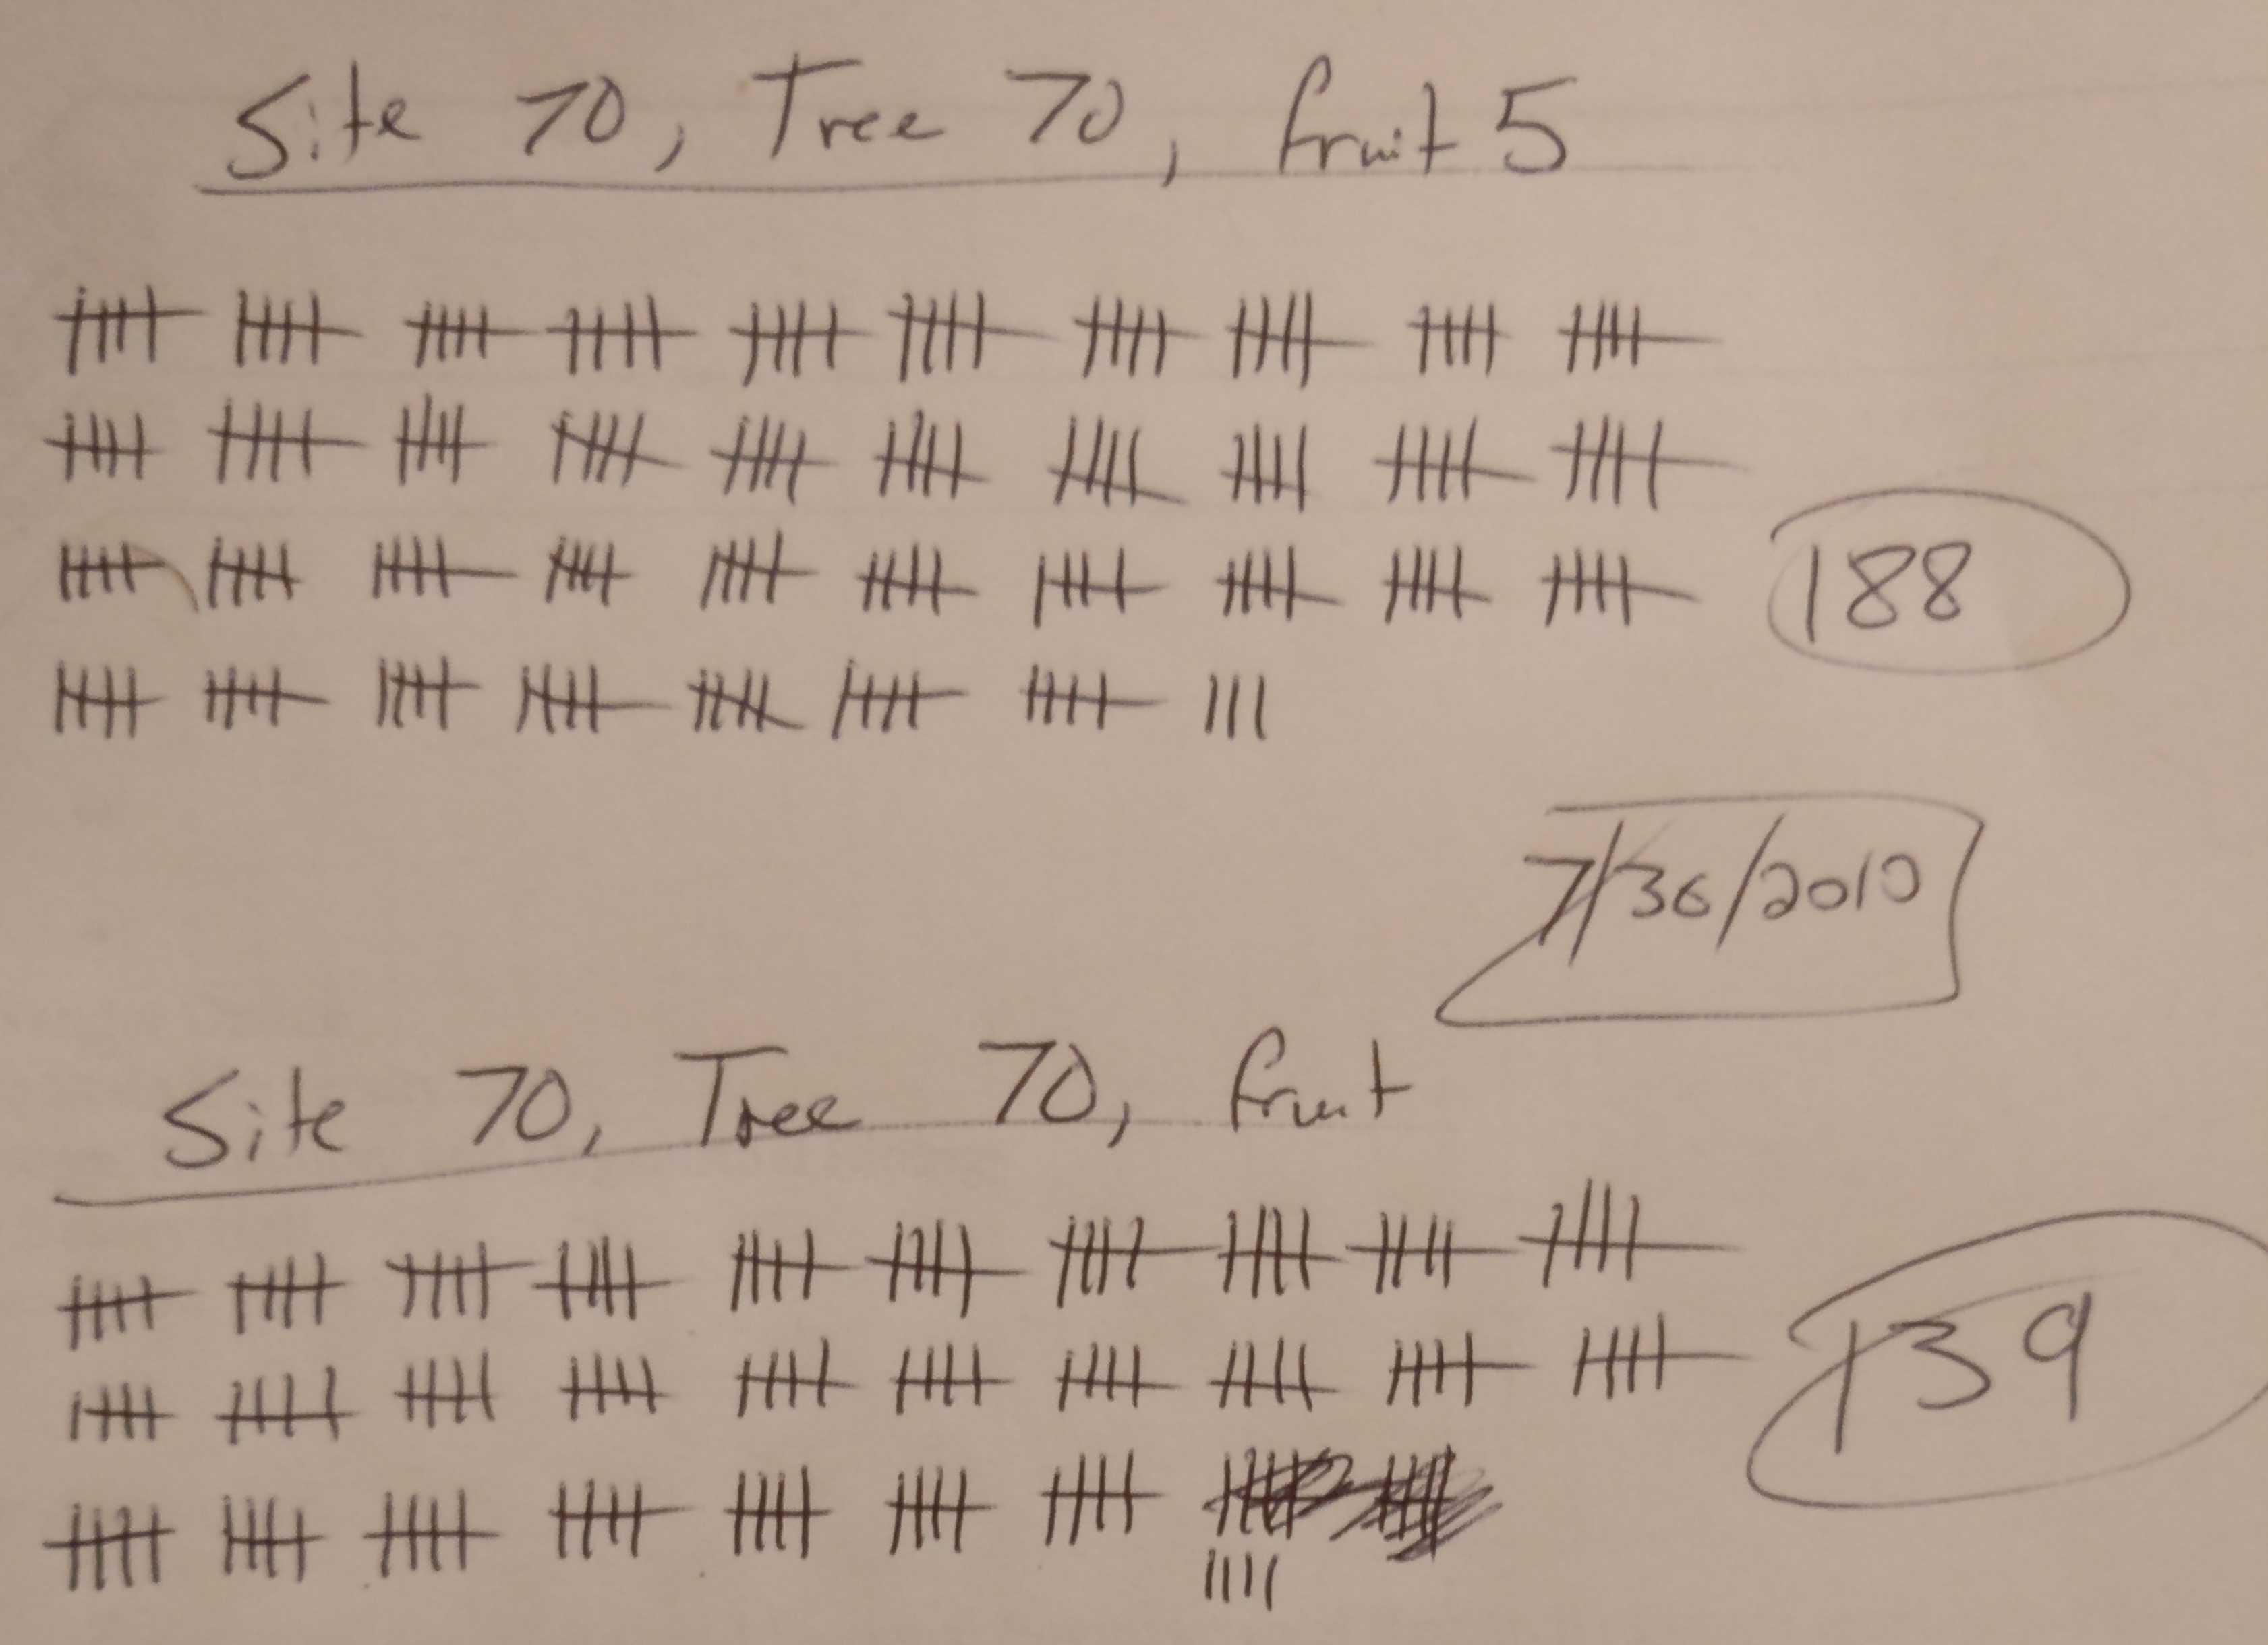
\includegraphics[width=1\linewidth]{img/Ch1_Ex1_seeds2} \caption{Tallies of seed counts collected from 2 fig fruits in Baja, Mexico in 2010.}\label{fig:unnamed-chunk-15}
\end{figure}

Fortunately, the summed tallies have been written and circled in the right margin of the notebook, which makes inputting them into a spreadsheet easier.
But it is important to also recognise this step as a potential source of human error in data collection.
It is possible that the tallies were counted inaccurately, meaning that the tallies on the left do not sum to the numbers in the right margins.
It is always good to be able to go back and check.
There are at least two other potential sources of human error in counting seeds and inputting them into the spreadsheet, one before, and one after counting the tallies.
Fill in 1 and 3 below with potential causes of error.

\begin{enumerate}
\def\labelenumi{\arabic{enumi}.}
\tightlist
\item
\item
  Tallies are not counted correctly in the lab notebook
\item
\end{enumerate}

Next, create a new column in the spreadsheet and call it ``Seeds'' (use column K).
Fill in the seed counts for each of the six rows.
The end result will be a tidy dataset that is ready to be saved as a CSV.

What you do next depends on the spreadsheet program that you are using and how you are using it.
If you are using LibreOffice Calc or MS Excel on a your computer, then you should be able to simply save your file as something like ``Fig\_fruits.csv'', and the program will recognise that you intend to save as a CSV file (in MS Excel, you might need to find the pulldown box for `Save as type:' under the `File name:' box and choose `CSV').
If you are using Google Sheets, you can navigate in the toolbar to \texttt{File\ \textgreater{}\ Download\ \textgreater{}\ Comma-separated\ values\ (.csv)}, which will start a download of your spreadsheet in CSV format.
If you are using MS Excel in a browser online, then it is a bit more tedious.
At the time of writing, the online version of MS Excel does not allow users to save or export to a CSV.
It will therefore be necessary to save as an XLSX, then convert to CSV later in another spreadsheet program (either a local version of MS Excel, LibreOffice Calc, or Google Sheets).

Save your file in a location where you know that you can find it again.
It might be a good idea to create a new folder on your computer or your cloud storage online for files in Statistical Techniques.
This will ensure that you always know where your data files are located and can access them easily.

\hypertarget{exercise-2-making-spreadsheet-data-tidy}{%
\section{Exercise 2: Making spreadsheet data tidy}\label{exercise-2-making-spreadsheet-data-tidy}}

Exercise 2 is more self-guided than Exercise 1.
After reading \protect\hyperlink{Chapter_2}{Chapter 2} and completing Exercise 1, you should have a bit more confidence in organising data in a tidy format.
Here we will work with a dataset that includes counts of the number of eggs collected from fig wasps, which are small species of insects that lay their eggs into the ovules of fig flowers \citep{Weiblen2002}.
You can \textbf{download the dataset \href{https://github.com/bradduthie/SCIU4T4/blob/main/data/wasp_egg_loads_untidy.xlsx?raw=true}{here}}, or recreate it from Figure 3.6.

\begin{figure}
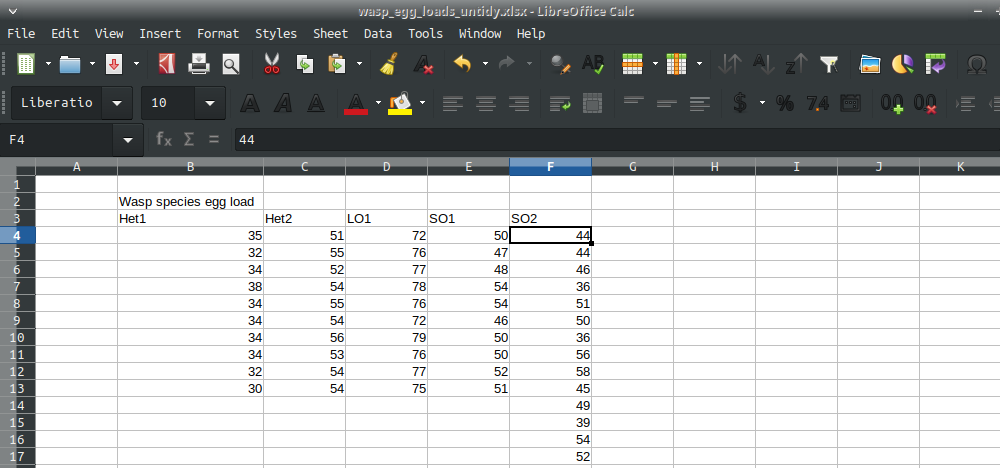
\includegraphics[width=1\linewidth]{img/wasp_egg_loads_untidy} \caption{An untidy dataset of egg loads from fig wasps of five different species, including two unnamed species of the genus *Heterandrium* (Het1 and Het2) and three unnamed species of the genus *Idarnes* (LO1, SO1, and SO2).}\label{fig:unnamed-chunk-16}
\end{figure}

Using what you have learned in \protect\hyperlink{Chapter_2}{Chapter 2} and Exercise 1, create a tidy version of the wasp egg loads dataset.
For a helpful hint, it might be most efficient to open a new spreadsheet and copy and paste information from the old to the new.

How many columns did you need to create the new dataset? \_\_\_\_\_\_\_\_\_

Are there any missing data in this dataset? \_\_\_\_\_\_\_\_\_

Save the tidy dataset to a CSV file.
It might be a good idea to check with classmates and an instructor to confirm that the dataset is in the correct format.

\hypertarget{exercise-3-making-data-tidy-again}{%
\section{Exercise 3: Making data tidy again}\label{exercise-3-making-data-tidy-again}}

Exercise 3, like Exercise 2, is self-guided.
The data are presented in a fairly common, but untidy, format, and the challenge is to reorganise them into a tidy dataset that is ready for statistical analysis.
Table 3.1 shows the number of different species of wasps counted in 5 different fig fruits.
Rows list all of the species and columns list the fruits, with the counts in the middle
This is an efficient way to present the data so that they are all easy to see, but this will not work for running statistical analysis.

\begin{longtable}[]{@{}lrrrrr@{}}
\caption{\label{tab:unnamed-chunk-17}An efficient but untidy way to present count data. Counts of different species of fig wasps (rows) are from 5 different fig fruits (columns). Data were originally collected from Baja, Mexico in 2010.}\tabularnewline
\toprule
Species & Fruit\_1 & Fruit\_2 & Fruit\_3 & Fruit\_4 & Fruit\_5 \\
\midrule
\endfirsthead
\toprule
Species & Fruit\_1 & Fruit\_2 & Fruit\_3 & Fruit\_4 & Fruit\_5 \\
\midrule
\endhead
Het1 & 0 & 0 & 0 & 1 & 0 \\
Het2 & 0 & 2 & 3 & 0 & 0 \\
LO1 & 4 & 37 & 0 & 0 & 3 \\
SO1 & 0 & 1 & 0 & 3 & 2 \\
SO2 & 1 & 12 & 2 & 0 & 0 \\
\bottomrule
\end{longtable}

This exercise might be a bit more challenging than Exercise 2.
The goal is to use the above information to create a tidy dataset.
Remember that each observation (wasp counts, in this case) should get its own row, and each variable should get its own column.
Try creating a tidy dataset from the information in Table 3.1, then save the dataset to a CSV file.
As with Exercise 2, it might be good to confer with classmates and an instructor to confirm that the dataset is in the correct format and will work for statistical analysis.

\hypertarget{exercise-4-tidy-data-and-spreadsheet-calculations}{%
\section{Exercise 4: Tidy data and spreadsheet calculations}\label{exercise-4-tidy-data-and-spreadsheet-calculations}}

Exercise 4 requires some restructuring and calculations.
The dataset that will be used in this exercise includes morphological measurements from five species of fig wasps, the same species used in Exercise 2.
\textbf{Download this dataset from the file \href{https://github.com/bradduthie/SCIU4T4/blob/main/data/wasp_morphology_untidy.xlsx?raw=true}{wasp\_morphology\_untidy.xlsx} (XLSX file) or \href{https://github.com/bradduthie/SCIU4T4/blob/main/data/wasp_morphology_untidy.ods?raw=true}{wasp\_morphology\_untidy.ods} (ODS open-source file).}
Both files contain identical information, so which one you use is a matter of personal preference.
This dataset is about as untidy as it gets.
First note that there are multiple sheets in the spreadsheet, which is not allowed in a tidy CSV file.
You can see these sheets by looking at the very bottom of the spreadsheet, which will have separating tabs called Het1, Het2, LO1, SO1, and SO2 (Figure 3.7).

\begin{figure}

\includegraphics[width=1\linewidth]{img/spreadsheet_tabs} \caption{Spreadsheets can include multiple sheets. This image shows that the spreadsheet containing information for fig wasp morphology includes five separate sheets, one for each species.}\label{fig:unnamed-chunk-18}
\end{figure}

You can click on all of the different tabs to see the measurements of head length, head width, thorax length, thorax width, abdomen length, and abdomen width for wasps of each of the 5 species.
All of the measurements are collected in millimeters.
Note that the individual sheets contain text formatting (titles highlighted, and in bold), and there is a picture of each wasp in its respective sheet.
The formatting and pictures are a nice touch for providing some context, but they cannot be used in statistical analysis.
The first task is to create a tidy version of this dataset.
Probably the best way to do this is to create a new spreadsheet entirely and copy-paste information from the old.
It is good idea to think about how the tidy dataset will look before getting started.
What columns should this new dataset include? Write your answer below.

\begin{verbatim}




\end{verbatim}

How many rows are needed? \_\_\_\_\_\_\_\_\_\_\_\_\_\_\_\_\_

When you are ready, create the new dataset.
Your dataset should have all of the relevant information about wasp head, thorax, and abdomen measurements.
It should look something like Figure 3.8.

\begin{figure}
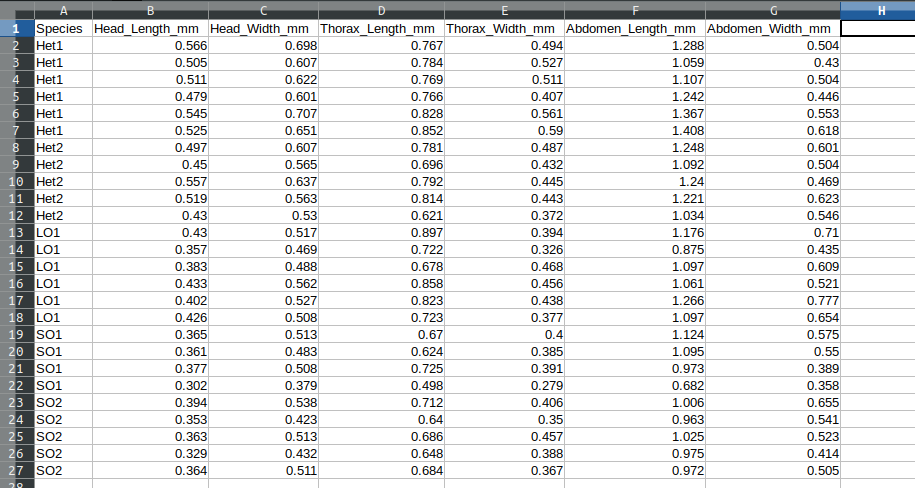
\includegraphics[width=1\linewidth]{img/Ch1_Ex3_tidy} \caption{A tidy dataset of wasp morphological measurements from 5 species of fig wasps collected from Baja, Mexico in 2010.}\label{fig:unnamed-chunk-19}
\end{figure}

Next comes a slightly more challenging part, which will make use of some of the background mathematics reviewed in \protect\hyperlink{Chapter_1}{Chapter 1}.
Suppose that we wanted our new dataset to include information about the volumes of each of the three wasp body segments, and wasp total volume.
To do this, let us assume that the wasp head is a sphere (it is not, exactly, but this is probably the best estimate that we can get under the circumstances).
Calculate the head volume of each wasp using the following formula,

\[V_{head} = \frac{4}{3}\pi \left(\frac{Head_L + Head_W}{4}\right)^{3}.\]

In the equation above, \(Head_{L}\) is head length (mm) and \(Head_{W}\) is head width (note, \((Head_L + Head_W)/4\) estimates the radius of the head).
You can replace \(\pi\) with the approximation \(\pi \approx 3.14\).
To make this calculation in your spreadsheet, find the cell in which you want to put the head volume.
By typing in the \texttt{=} sign, the spreadsheet will know to start a new calculation or function in that cell.
Try this with an empty cell by typing ``\texttt{=\ 5\ +\ 4}'' in it (without quotes).
When you hit `Enter', the spreadsheet will make the calculation for you and the number in the new cell will be 9.
To see the equation again, you just need to double-click on the cell.

To get an estimate of head volume into the dataset, we can create a new column of data.
To calculate \(V_{head}\) for the first wasp in row 2 of Figure 3.8, we could select the spreadsheet cell H2 and type the code, \texttt{=(4/3)*(3.14)*((B2+C2)/4)\^{}3}.
Notice that the code recognises \texttt{B2} and \texttt{C2} as spreadsheet cells, and takes the values from these cells when doing these calculations.
If the values of \texttt{B2} or \texttt{C2} were to change, then so would the calculated value in H2.
Also notice that we are using parentheses to make sure that the order of operations is correct.
We want to add head length and width before dividing by 4, so we type \texttt{((B2+C2)/4)} to ensure with the innermost parentheses that head length and width are added before dividing.
Once all of this is completed, we raise everything in parentheses to the third power using the \texttt{\^{}3}, so \texttt{((B2+C2)/4)\^{}3}.
Different mathematical operations can be carried out using the the symbols in Table 3.2.

\begin{longtable}[]{@{}ll@{}}
\caption{List of mathematical operations available in a spreadsheet.}\tabularnewline
\toprule
Symbol & Operation \\
\midrule
\endfirsthead
\toprule
Symbol & Operation \\
\midrule
\endhead
\texttt{+} & Addition \\
\texttt{-} & Subtraction \\
\texttt{*} & Multiplication \\
\texttt{/} & Division \\
\texttt{\^{}} & Exponent \\
\texttt{sqrt()} & Square-root \\
\bottomrule
\end{longtable}

The last operation in Table 3.2 is a function that takes the square-root of anything within the parentheses.
Other functions are also available that can make calculations across cells (e.g., \texttt{=SUM} or \texttt{=AVERAGE}), but we will ignore these for now.

Once head volume is calculated for the first wasp in cell H2, it is very easy to do the rest.
One nice feature of a spreadsheet is that it can usually recognise when the cells need to change (B2 and C2, in this case).
To get the rest of the head volumes, we just need to select the bottom right of the H2 cell.
There will be a very small square in this bottom right (see Figure 3.9), and if we drag it down, the spreadsheet will do the same calculation for each row (e.g., in H3, it will use B3 and C3 in the formula rather than B2 and C2).

\begin{figure}
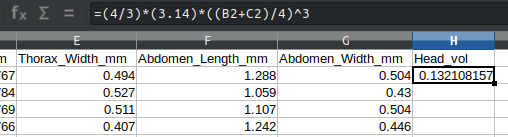
\includegraphics[width=1\linewidth]{img/Ch1_Ex3_copy_formula} \caption{A dataset of wasp morphological measurements from 5 species of fig wasps collected from Baja, Mexico in 2010. Head volume (column H) has been calculated for row 2, and to calculate it for the remaining rows, the small black square in the bottom right of the highlighted cell H2 can be clicked and dragged down to H27.}\label{fig:unnamed-chunk-20}
\end{figure}

Another way to achieve the same result is to copy (Ctrl + C) the contents of cell H2, highlight cells H3-H27, then paste (Ctrl + V).
However you do it, you should now have a new column of calculated head volume.

Next, suppose that we want to calculate thorax and abdomen volumes for all wasps.
Unlike wasp heads, wasp thoraxes and abdomens are clearly not spheres.
But it is perhaps not entirely unreasonable to model them as ellipses.
To calculate wasp thorax and abdomen volumes assuming an ellipse, we can use the formula,

\[V_{thorax} = \frac{4}{3}\pi \left(\frac{Thorax_{L}}{2}\right)\left(\frac{Thorax_{W}}{2}\right)^{2}.\]
In the equation above, \(Thorax_{L}\) is thorax length (mm) and \(Thorax_{W}\) is thorax width.
Substitute \(Abdomen_{L}\) and \(Abdomen_{W}\) to instead calculate abdomen volume (\(V_{abdomen}\)).
What formula will you type into your empty spreadsheet cell to calculate \(V_{thorax}\)? Keep in mind the order of operations indicated in the equation above.

\begin{verbatim}




\end{verbatim}

Now fill in the columns for thorax volume and abdomen volume.
You should now have 3 new columns of data from calculations of the volumes of the head, thorax, and abdomen of each wasp.
Lastly, add 1 final column of data for total volume, which is the sum of the 3 segments.

There are a lot of potential sources of error and uncertainty in these final volumes.
What are some reasons that we might want to be cautious about our calculated wasp volumes?
Explain in 2-3 sentences.

\begin{verbatim}




\end{verbatim}

Save your wasp morphology file as a CSV.
This was the last exercise of the practical.
You should now be comfortable formatting tidy datasets for use in statistical software.
Next week, we will begin using Jamovi to do some descriptive statistics and plotting.

\hypertarget{summary}{%
\section{Summary}\label{summary}}

Completing this practical should give you the skills that you need to prepare datasets for statistical analysis.
There are many additional features of spreadsheets that were not introduced (mainly because we will do them in Jamovi), but could be useful to learn.
For example, if we wanted to calculate the sum of all head lengths, we could use the function \texttt{=sum(B2:B27)} in any spreadsheet cell (where B2 is the head length of the first wasp, and B27 is the head length of the last wasp).
Other functions such as \texttt{=count()}, \texttt{=min()}, \texttt{=max()}, or \texttt{=average()} can be similarly used for calculations.
If you have time at the end of the lab, we recommend exploring the spreadsheet interface and seeing what you can do.

\hypertarget{part-statistical-concepts}{%
\part{Statistical concepts}\label{part-statistical-concepts}}

\hypertarget{Week2}{%
\chapter*{Week 2 Overview}\label{Week2}}
\addcontentsline{toc}{chapter}{Week 2 Overview}

\begin{longtable}[]{@{}
  >{\raggedright\arraybackslash}p{(\columnwidth - 2\tabcolsep) * \real{0.3269}}
  >{\raggedright\arraybackslash}p{(\columnwidth - 2\tabcolsep) * \real{0.6731}}@{}}
\toprule
\endhead
\textbf{Dates} & 30 January 2023 - 3 February 2023 \\
\textbf{Reading} & \textbf{Required:} SCIU4T4 Workbook chapters 4-7 \\
& \textbf{Recommended:} \citet{Navarro2022} \href{https://davidfoxcroft.github.io/lsj-book/getting-started-with-jamovi.html\#the-spreadsheet}{Section 3.3}-\href{https://davidfoxcroft.github.io/lsj-book/getting-started-with-jamovi.html\#summary-1}{3.9} \\
& \textbf{Suggested:} \citet{Rowntree2018} Chapter 2 \\
& \textbf{Advanced:} None \\
\textbf{Lectures} & 2.0: Why study statistics? (18:13 min; \href{https://stirling.cloud.panopto.eu/Panopto/Pages/Viewer.aspx?id=9d251ac5-f4a3-4b06-bf15-af8200d91518}{Video}) \\
& 2.1: Populations and samples (6:47 min; \href{https://stirling.cloud.panopto.eu/Panopto/Pages/Viewer.aspx?id=b248a69a-8831-4098-94ce-af8200d91544}{Video}) \\
& 2.2: Types of variables (11:00 min; \href{https://stirling.cloud.panopto.eu/Panopto/Pages/Viewer.aspx?id=b7016026-20c8-4237-afba-af8200d915b5}{Video}) \\
& 2.3: Units, precision, and accuracy (9:06 min; \href{https://stirling.cloud.panopto.eu/Panopto/Pages/Viewer.aspx?id=4a9915ad-bfe9-4f1a-928c-af8200d915d8}{Video}) \\
& 2.4: Uncertainty propagation (11:44 min; \href{https://stirling.cloud.panopto.eu/Panopto/Pages/Viewer.aspx?id=4d913c54-8b80-487c-9632-af8200d91630}{Video}) \\
\textbf{Practical} & Introduction to Jamovi (\protect\hyperlink{Chapter_8}{Chapter 8}) \\
& Room: Cottrell 2A17 \\
& Group A: 01 FEB 2023 (WED) 13:05-15:55 \\
& Group B: 02 FEB 2023 (THU) 09:05-11:55 \\
\textbf{Help hours} & Ian Jones \\
& Room: Cottrell 1A13 \\
& 03 FEB 2023 (FRI) 15:05-17:55 \\
\textbf{Assessments} & \href{https://canvas.stir.ac.uk/courses/13075/quizzes/29673}{Week 2 Practice quiz} on Canvas \\
\bottomrule
\end{longtable}

Week 2 focuses on general statistical concepts, data, and measurement.

\protect\hyperlink{Chapter_4}{Chapter 4} focuses on key concepts that will be used throughout this module.
In particular, it is important to understand the difference between a \textbf{population} and a \textbf{sample}, and to recognise that there are many types of variables in statistics.

\protect\hyperlink{Chapter_5}{Chapter 5} introduces different variable types. Different types of variables have different characteristics, which will affect how these variables are best visualised in figures and analysed with statistical hypothesis tests introduced later in the semester.
A variable's type will rarely be stated explicitly when doing scientific research, and will not always be provided in assessments for this module.
Being able to infer variable type is therefore an important skill.

\protect\hyperlink{Chapter_6}{Chapter 6} focuses on units of measurement, and how these units are communicated in text.
Units are essential in scientific measurement, and we will use them throughout the module to indicate the type and scale of data measurement.
We are not expecting you to memorise all scientific units, so a \protect\hyperlink{appendixA_units}{table on units} is provided.

\protect\hyperlink{Chapter_7}{Chapter 7} will introduce the propogation of measurement errors.
This is important to understand because no measurement is perfectly accurate, and predicting how errors in measurement combine is fundamental to understanding measurement accuracy.

\protect\hyperlink{Chapter_8}{Chapter 8} guides you through the Week 2 practical, which is an introduction to Jamovi.
This aim of this practical is to become familiar with the Jamovi interface and comfortable importing data into Jamovi to collect some descriptive statistics.

\hypertarget{Chapter_4}{%
\chapter{Populations and samples}\label{Chapter_4}}

When we collect data, we are recording some kind of observation or measurement.
If we are working in a forest, for example, we might want to measure the heights of different trees, or measure the concentration of carbon in the soil.
The idea might be to use these measurements to make some kind of inference about the forest.
But as scientists, we are almost always limited in the amount of data that we can collect.
We cannot measure everything, so we need to collect a \emph{sample} of data and use it to make inferences about the \emph{population} of interest.
For example, while we probably cannot measure the height of every tree in a forest, nor can we measure the concentration of carbon at every possible location in the forest's soil, we can collect a smaller number of measurements and still make useful conclusions about overall forest tree height and carbon concentration.

Statistics thereby allows us to approximate properties of entire populations from a limited number of samples.
This needs to be done with caution, but before getting into the details of how, it is important to fully understand the difference between a \textbf{population} and a \textbf{sample} to avoid confusing these two concepts.
A \textbf{population} is the entire set of possible observations that could be collected.
Some examples will make it easier to understand:

\begin{itemize}
\tightlist
\item
  All of the genes in the human genome
\item
  All individuals of voting age in Scotland
\item
  All common pipistrelle bats in the United Kingdom
\end{itemize}

These populations might be important for a particular research question.
For example, we might want to know something about the feeding behaviours of pipistrelle bats in the UK.
But there is no way that we can find and observe the behaviour of every single bat, so we need to take a subset of the population (a sample) instead.
Examples of samples include the following:

\begin{itemize}
\tightlist
\item
  A selection of 20 human genes
\item
  A pub full of Scottish voters
\item
  40 caught common pipistrelle bats
\end{itemize}

It is important to recognise that the word ``population'' means something slightly different in statistics than it does in biology.
A biological population, for example, could be defined as all of the individuals of the same species in the same general location.
A statistical population, in contrast, refers to a set of observations (i.e., things that we can measure).
\citet{Sokal1995} provide a more technical definition for ``population'',

\begin{quote}
In statistics, population always means the \emph{totality of individual observations about which inferences are to be made, existing anywhere in the world or at least within a definitely specified sampling area limited in space and time} {[}p.~9, emphasis theirs{]}.
\end{quote}

They define a sample to be ``a collection of individual observations selected by a specified procedure'' \citep{Sokal1995}.
For our purposes, it is not necessary to be able to recite the technical definitions, but it is important to understand the relationship between a population and a sample.
When we collect data, we are almost always taking a small sample of observations from a much larger number of possible observations in a population.

\begin{figure}
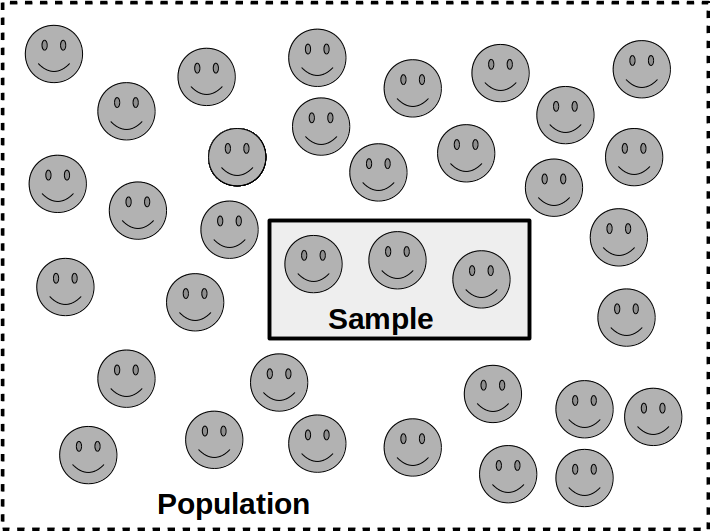
\includegraphics[width=1\linewidth]{img/population_vs_sample} \caption{A conceptual figure illustrating how a statistical population relates to a statistical sample. The population is represented by 35 smiling faces enclosed within a dashed box. The sample is represented by a solid box within the dashed box, within which there are 3 smiling faces. Hence, we have a sample of 3 measurements from the total population.}\label{fig:unnamed-chunk-21}
\end{figure}

\hypertarget{Chapter_5}{%
\chapter{Types of variables}\label{Chapter_5}}

A variable is any property that is measured in an observation \citep{Sokal1995}; i.e., anything that varies among things that we can measure \citep{Dytham2011}.
We can summarise how these measurements vary with summary statistics, or visually with figures.
Often, we will want to predict one variable from a second variable.
In this case, the variable that we want to predict is called the \textbf{response variable}, also known as the \textbf{dependent variable} or \textbf{Y} variable (`dependent' because it \emph{depends} on other variables, and `Y' because this is the letter we often use to represent it).
The variable that we use to predict our response variable is the \textbf{explanatory variable}, also known as the \textbf{independent variable} or \textbf{X} variable (`independent' because it does not depend on other variables, and `X' because this is the letter most often used to represent it).
There are several different types of variables:

\begin{itemize}
\item
  \textbf{Categorical} variables take on a fixed number of discrete values \citep{Spiegelhalter2019}.
  In other words, the measurement that we record will assign our data to a specific category.
  Examples of categorical variables include species (e.g., ``Robin'', ``Nightingale'', ``Wren'') or life history stage (e.g., ``egg'', ``juvenile'', ``adult'').
  Categorical variables can be either nominal or ordinal.

  \begin{itemize}
  \tightlist
  \item
    \textbf{Nominal} variables do not have any inherent order (e.g., classifying land as ``forest'', ``grassland'', or ``urban'').
  \item
    \textbf{Ordinal} variables do have an inherent order (e.g., ``low'', ``medium'', and ``high'' elevation).
  \end{itemize}
\item
  \textbf{Quantitative} variables are variables represented by numbers that reflect a magnitude.
  That is, unlike categorical variables, we are collecting numbers that really mean something tangible (in contrast, while we might represent low, medium, and high elevations with the numbers 1, 2, and 3, respectively, this is just for convenience; a value of `2' does not always mean `medium' in other contexts).
  Categorical variables can be either discrete or continuous.

  \begin{itemize}
  \item
    \textbf{Discrete} variables can take only certain values.
    For example, if we want to record the number of species in a forest, then our variable can only take discrete counts (i.e., integer values).
    There could conceivably be any natural number of species (1, 2, 3, etc.), but there could not be 2.51 different species in a forest; that does not make sense.
  \item
    \textbf{Continuous} variables can take any real value within some range of values (i.e., any number that can be represented by a decimal).
    For example, we could measure height to as many decimals as our measuring device will allow, with a range of values from zero to the maximum possible height of whatever it is we are measuring.
    Similarly, we could measure temperature to any number of decimals, at least in theory, so temperature is a continuous variable.
  \end{itemize}
\end{itemize}

The reason for organising variables into all of these different types is that different types of variables need to be handled in different ways.
For example, it would not make sense to visualise a nominal variable in the same way as a continuous variable.
Similarly, the choice of statistical test to apply to answer a statistical question will almost always depend on the types of variables involved.
If presented with a new data set, it is therefore very important to be able to interpret the different variables and apply the correct statistical techniques (this will be part of the assessment for this module).

\hypertarget{Chapter_6}{%
\chapter{Accuracy, precision, and units}\label{Chapter_6}}

The science of measurements is called ``metrology'', which, among other topics, focuses on measurement accuracy, precision, and units \citep{Rabinovich2013}.
We will not discuss these topics in depth, but they are important for statistical techniques because measurement, in the broadest sense of the word, is the foundation of data collection.
When collecting data, we want measurements to be accurate, precise, and clearly defined.

\hypertarget{accuracy}{%
\section{Accuracy}\label{accuracy}}

When we collect data, we are trying to obtain information about the world.
We might, for example, want to know the number of seedlings in an area of forest, the temperature of the soil at some location, or the mass of a particular animal in the field.
To get this information, we need to make measurements.
Some measurements can be collected by simple observation (e.g., counting seedlings), while others will require measuring devices such as a thermometer (for measuring temperature) or scale (for measuring mass).
All of these measurements are subject to error.
The \emph{true} value of whatever it is that we are trying to measure (called the ``measurand'') can differ from what we record when collecting data.
This is true even for simple observations (e.g., we might miscount seedlings), so it is important to recognise that the data we collect comes with some uncertainty.
The \textbf{accuracy} of a measurement is defined by how close the measurement is to the \emph{true} value of what we are trying to measure \citep{Rabinovich2013}.

\hypertarget{precision}{%
\section{Precision}\label{precision}}

The \textbf{precision} of a measurement is how consistent it will be if measurement is replicated multiple times.
In other words, precision describes how similar measurements are expected to be.
If, for example, a scale measures an object to be the exact same mass every time it is weighed (regardless of whether the mass is accurate), then the measurement is highly precise.
If, however, the scale measures a different mass each time the object is weighed (for this hypothetical, assume that the true mass of the object does not change), then the measurement is not as precise.

One way to visualise the difference between accuracy and precision is to imagine a set of targets, with the centre of the target representing the true value of what we are trying to measure (Figure 6.1)\footnote{This figure was released into the public domain by \href{https://commons.wikimedia.org/wiki/File:Accuracy-vs-precision-nl.svg}{Egon Willighagen} on 8 March 2014.}.

\begin{figure}
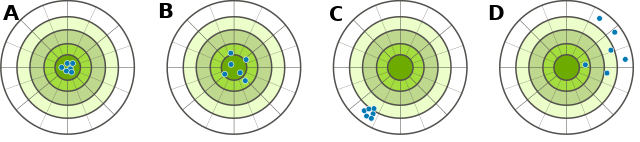
\includegraphics[width=1\linewidth]{img/accuracy_vs_precision} \caption{A conceptual figure illustrating the difference between accuracy and precision. Points in (A) are both accurate and precise, points in (B) are accurate, but not precise, points in (C) are precise but not accurate, and points in (D) are neither accurate nor precise.}\label{fig:unnamed-chunk-22}
\end{figure}

Note again that accuracy and precision are not necessarily the same.
Measurement can be accurate but not precise (Figure 6.1B) or precise but not accurate (Figure 6.1C).

\hypertarget{systems-of-units}{%
\section{Systems of units}\label{systems-of-units}}

Scientific units are standardised with the Système International D'Unités (SI).
Having standardised units of measurement is highly important to ensure measurement accuracy \citep{Quinn1995}.
Originally, these units were often defined in terms of physical artefacts.
For example, the kilogram (kg) was once defined by a physical cylinder of metal housed in the Bureau International des Poids et Mesures (BIPM).
In other words, the mass of a metal sitting at the BIPM \emph{defined} what a kg was, with the mass of every other measurement being based on this physical object \citep{Quinn1995}.
This can potentially present a problem if the mass of that one object changes over time, thereby causing a change in how a kg is defined.
Where possible, it is therefore preferable to define units in terms of fundamental constants of nature.
In 2019, for example, the kg was redefined in terms of the Planck constant, a specific atomic transition frequency, and the speed of light \citep{Stock2019}.
This ensures that measurements of mass remain accurate over time because what a kg represents in terms of mass cannot change.

We can separate units into base units and derived units.
Table 6.1 below lists some common base units for convenience \citep{Quinn1995}.
You do not need to memorise these units, but it is good to be familiar with them.
We will use these units throughout the module.

\begin{longtable}[]{@{}lll@{}}
\caption{Base units of SI measurements. For details see \citet{Quinn1995}.}\tabularnewline
\toprule
\textbf{Measured Quantity} & \textbf{Name of SI unit} & Symbol \\
\midrule
\endfirsthead
\toprule
\textbf{Measured Quantity} & \textbf{Name of SI unit} & Symbol \\
\midrule
\endhead
Mass & kilogram & \(kg\) \\
Length & metre & \(m\) \\
Time & second & \(s\) \\
Electric current & ampere & \(A\) \\
Temperature & kelvin & \(K\) \\
Amount of a substance & mole & \(mol\) \\
Luminous intensity & candela & \(cd\) \\
\bottomrule
\end{longtable}

We can also define derived SI units from the base units of Table 6.1; examples of these derived SI units are provided in Table 6.2.
Again, you do not need to memorise these units, but it is good to be aware of them.

\begin{longtable}[]{@{}
  >{\raggedright\arraybackslash}p{(\columnwidth - 8\tabcolsep) * \real{0.2000}}
  >{\raggedright\arraybackslash}p{(\columnwidth - 8\tabcolsep) * \real{0.1565}}
  >{\raggedright\arraybackslash}p{(\columnwidth - 8\tabcolsep) * \real{0.1043}}
  >{\raggedright\arraybackslash}p{(\columnwidth - 8\tabcolsep) * \real{0.2435}}
  >{\raggedright\arraybackslash}p{(\columnwidth - 8\tabcolsep) * \real{0.2957}}@{}}
\caption{Examples of derived SI units.}\tabularnewline
\toprule
\begin{minipage}[b]{\linewidth}\raggedright
\textbf{Measured Quantity}
\end{minipage} & \begin{minipage}[b]{\linewidth}\raggedright
\textbf{Name of unit}
\end{minipage} & \begin{minipage}[b]{\linewidth}\raggedright
\textbf{Symbol}
\end{minipage} & \begin{minipage}[b]{\linewidth}\raggedright
\textbf{Definition in SI units}
\end{minipage} & \begin{minipage}[b]{\linewidth}\raggedright
\textbf{Alternative in derived units}
\end{minipage} \\
\midrule
\endfirsthead
\toprule
\begin{minipage}[b]{\linewidth}\raggedright
\textbf{Measured Quantity}
\end{minipage} & \begin{minipage}[b]{\linewidth}\raggedright
\textbf{Name of unit}
\end{minipage} & \begin{minipage}[b]{\linewidth}\raggedright
\textbf{Symbol}
\end{minipage} & \begin{minipage}[b]{\linewidth}\raggedright
\textbf{Definition in SI units}
\end{minipage} & \begin{minipage}[b]{\linewidth}\raggedright
\textbf{Alternative in derived units}
\end{minipage} \\
\midrule
\endhead
Energy & Joule & \(J\) & \(m^{2}\) \(kg\) \(s^{-2}\) & \(N\) \(m\) \\
Force & Newton & \(N\) & \(m\) \(kg\) \(s^{-2}\) & \(J\) \(m^{-1}\) \\
Pressure & Pascal & \(Pa\) & \(kg\) \(m^{-1}\) \(s^{-2}\) & \(N\) \(m^{-2}\) \\
Power & Watt & \(W\) & \(m^{-2}\) \(kg\) \(s^{-3}\) & \(J\) \(s^{-1}\) \\
Frequency & Hertz & \(Hz\) & \(s^{-1}\) & \\
Radioactivity & Becquerel & \(Bq\) & \(s^{-1}\) & \\
\bottomrule
\end{longtable}

When numbers are associated with units, it is important to recognise that the units must be carried through and combined when calculating an equation.
As a very simple example, if want to know the speed at which an object is moving, and we find that it has moved 10 metres in 20 seconds, then we calculate the speed and report the correct units as below,

\[speed = \frac{10\:m}{20\:s} = 0.5\:m/s = 0.5\:m\:s^{-1}.\]

Notice that the final units are in metres per second, which can be written as \(m/s\) or \(m\:s^{-1}\) (remember that raising \(s\) to the \(-1\) power is the same as \(1/s\); see \protect\hyperlink{Chapter_1}{Chapter 1} for a quick reminder about superscripts).
It is a common error to calculate just the numeric components of a calculation and ignore the associated units.
Often on assessments, we will ask you not to include units in your answer (this is just for convenience on the tests and exam), but recognising that units are also part of calculations is important.

\hypertarget{other-examples-of-units}{%
\section{Other examples of units}\label{other-examples-of-units}}

Remember that an exponent (indicated by a superscript, e.g., the 3 in \(m^{3}\)) indicates the number of times to multiply a base by itself, so \(m^{3} = m \times m \times m\).

\hypertarget{units-of-density}{%
\subsection{Units of density}\label{units-of-density}}

Density (\(\rho\)) is calculated by,

\[\rho = \frac{mass}{volume} = \frac{kg}{m^{3}}.\]

The units of density are therefore mass per unit volume, \(kg\:m^{-3}\).

\hypertarget{mass-of-metal-discharged-from-a-catchment}{%
\subsection{Mass of metal discharged from a catchment}\label{mass-of-metal-discharged-from-a-catchment}}

The mass of metal carried by a stream per unit time (\(M\)) is given by multiplying the concentration of metal per unit volume (\(C\)) of water by the volume of water discharged per unit time (\(V\)),

\[M = C \times V.\]
This equation is useful in showing how units can cancel each other out.
If we calculate the above with just the units (ignoring numbers for \(C\) and \(V\)),

\[M = \frac{mg}{l} \times \frac{l}{s} = \frac{mg}{s}.\]

Notice above how the \(l\) units on the top and bottom of the equation cancel each other out, so we are left with just \(mg/s\).

\hypertarget{soil-carbon-inventories}{%
\subsection{Soil carbon inventories}\label{soil-carbon-inventories}}

For one final example, the inventory of carbon \(I\) within a soil is given by the specific carbon concentration \(C\) (\(g\) of carbon per \(kg\) of soil), multiplied by the depth of soil analysed (\(D\), measured in \(m\)), and by the density (\(\rho\), measured in \(kg\:m^{-3}\)),

\[I = C \times D \times \rho = \frac{g\times m \times kg}{kg \times m^{3}} = \frac{g}{m^{2}} = g\:m^{-2}.\]
Notice above how the \(kg\) on the top and bottom of the fraction cancel each other out, and how one \(m\) on the top cancels out one \(m\) on the bottom, so that what we are left with is grams per metre squared (\(g\:m^{-2}\)).

\hypertarget{Chapter_7}{%
\chapter{Uncertainty propogation}\label{Chapter_7}}

Nothing can be measured with perfect accuracy, meaning that every measurement has some associated error.
The measurement error might be caused by random noise in the measuring environment, or by mistakes made by the person doing the measuring.
The measurement error might also be caused by limitations or imperfections associated with a measuring device.
The device might be limited in its measurement precision, or perhaps it is biased in its measurements due to improper calibration, manufacture, or damage from previous use.
All of this generates uncertainty with respect to individual measurements.

Recall from \protect\hyperlink{Chapter_6}{Chapter 6} the difference between precision and accuracy.
We can evaluate the precision and accuracy of measurements in different ways.
Measurement precision can be estimated by replicating a measurement (i.e., taking the same measurement over and over again).
The more replicate measurements made, the more precisely a value can be estimated.
For example, if we wanted to evaluate the precision with which the mass of an object is measured, then we might repeat the measurement with the same scale multiple times and see how much mass changes across different measurements.
To evaluate measurement accuracy, we might need to measure a value in multiple different ways (e.g., with different measuring devices).
For example, we might repeat the measurement of an object's mass with a different scale (i.e., a different physical scale used for measuring the mass of objects).

Sometimes it is necessary to combine different measured values.
For example, we might measure the mass of 2 different bird eggs in a nest separately, then calculate the total mass of both the 2 eggs combined.
The measurement of each egg will have its own error, and these errors will propagate to determine the error of the total egg mass for the nest.
How this error propagates differs depending on if they are being added or subtracted, or if they are being multiplied or divided.

\hypertarget{adding-or-subtracting-errors}{%
\section{Adding or subtracting errors}\label{adding-or-subtracting-errors}}

In the case of our egg masses, we can assign the mass of the first egg to the variable \(X\) and the mass of the second egg to the variable \(Y\).
We can assign the total mass to the variable \(Z\), where \(Z = X + Y\).
The errors associated with the variables \(X\), \(Y\), and \(Z\) can be indicated by \(E_{X}\), \(E_{Y}\), and \(E_{Z}\), respectively.
In general, if the variable \(Z\) is calculated by adding (or subtracting) 2 or more values together, then this is the formula for calculating \(E_{Z}\),

\[E_{Z} = \sqrt{E^{2}_{X} + E^{2}_{Y}}.\]

Hence, for the egg masses, the error of the combined masses (\(E^{2}_{Z}\)) equals the square root of the error associated with the mass of egg 1 squared (\(E^{2}_{X}\)) plus the error associated with the mass of egg 2 squared (\(E^{2}_{Y}\)).
It often helps to provide a concrete example.
If the error associated with the measurement of egg 1 is \(E^{2}_{X} = 2\), and the error associated with the measurement of egg 2 is \(E^{2}_{Y} = 3\), then we can calculate,

\[E_{Z} = \sqrt{2^{2} + 3^{2}} \approx 3.61.\]

Note that the units of \(E_{Z}\) are the same as \(Z\) (e.g., grams).

\hypertarget{multiplying-or-dividing-errors}{%
\section{Multiplying or dividing errors}\label{multiplying-or-dividing-errors}}

Multiplying or dividing errors works a bit differently.
As an example, suppose that we need to measure the total area of a rectangular field.
If we measure the length (\(L\)) and width (\(W\)) of the field, then the total area is the product of these measurements, \(A = L \times W\).
Again, there is going to be error associated with the measurement of both length (\(E_{L}\)) and width (\(E_{W}\)).
How the error of the total area (\(E_{A}\)) is propagated by \(E_{L}\) and \(E_{W}\) is determined by the formula,

\[E_{A} = A \sqrt{\left(\frac{E_{L}}{L} \right)^{2} + \left(\frac{E_{W}}{W} \right)^{2}}.\]
Notice that just knowing the error of each measurement (\(E_{L}\) and \(E_{W}\)) is no longer sufficient to calculate the error associated with the measurement of the total area.
We also need to know \(L\), \(W\), and \(A\).
If our field has a length of \(L = 20\) m and width of \(W = 10\) m, then \(A = 20 \times 10 = 200\:m^{2}\).
If length and width measurements have associated errors of \(E_{L} = 2\) m and \(E_{W} = 1\) m, then,

\[E_{A} = 200 \sqrt{\left(\frac{2}{20} \right)^{2} + \left(\frac{1}{10} \right)^{2}} \approx 28.3\:m^{2}.\]

Of course, not every set of measurements with errors to be multiplied will be lengths and widths (note, however, that the units of \(E_{A}\) are the same as \(A\), \(m^{2}\)).
To avoid confusion, the general formula for multiplying or dividing errors is below, with the variables \(L\), \(W\), and \(A\) replaced with \(X\), \(Y\), and \(Z\), respectively, to match the case of addition and subtraction explained above,

\[E_{Z} = Z \sqrt{\left(\frac{E_{X}}{X} \right)^{2} + \left(\frac{E_{Y}}{Y} \right)^{2}}.\]

Note that the structure of the equation is the exact same, just with different letters used as variables.
It is necessary to be able to apply these equations correctly to estimate combined error.

\hypertarget{applying-formulas-for-combining-errors}{%
\section{Applying formulas for combining errors}\label{applying-formulas-for-combining-errors}}

It is not necessary to understand why the equations for propagating different types of errors are different, but a derivation is provided in \protect\hyperlink{uncertainty_derivation}{Appendix B} for the curious.

\hypertarget{Chapter_8}{%
\chapter{Practical. Introduction to Jamovi}\label{Chapter_8}}

This practical focuses on learning how to work with datasets in Jamovi.
Jamovi is available in the university laboratory computers through AppsAnywhere.
You can also \href{https://www.jamovi.org/download.html}{download it} on your own computer for free or run it directly \href{https://www.jamovi.org/cloud.html}{from a browser}.
For an introduction to what Jamovi is and why we are using it in this module, see the introduction of this workbook and \href{https://davidfoxcroft.github.io/lsj-book/03-Getting-started-with-jamovi.html\#the-spreadsheet}{Sections 3.3}-\href{https://davidfoxcroft.github.io/lsj-book/03-Getting-started-with-jamovi.html\#summary}{3.9} of \citet{Navarro2022}.
In this practical, we will work with two datasets, both of which are based on real biological and environmental studies conducted by researchers at the University of Stirling.

The first dataset includes measurements of soil organic carbon (grams of Carbon per kg of soil) from the topsoil and subsoil collected in a national park in Gabon.
These data were collected by Dr Carmen Rosa Medina-Carmona in an effort to understand how \href{https://bg.copernicus.org/articles/3/397/2006/bg-3-397-2006.pdf}{pyrogenic carbon} (i.e., carbon produced by the charring of biomass during a fire) is stored in different landscape areas \citep{Santin2016, Preston2006}.
\textbf{Download these data here: \href{https://raw.githubusercontent.com/bradduthie/SCIU4T4/main/data/soil_organic_carbon.csv}{soil\_organic\_carbon.csv}} (right click and ``Save Link As\ldots{}'').

The second dataset includes measurements of figs from trees of the Sonoran Desert Rock Fig (\emph{Ficus petiolaris}) in Baja, Mexico.
These data were collected by Dr Brad Duthie in an effort to understand coexistence in a fig wasp community \citep{Duthie2015b, Duthie2016}.
Measurements include fig lengths, widths, and heights in centimeters from 4 different fig trees, and the number of seeds in each fruit.
\textbf{Download these data here: \href{https://raw.githubusercontent.com/bradduthie/SCIU4T4/main/data/fig_fruits.csv}{fig\_fruits.csv}} (right click and ``Save Link As\ldots{}'').

\begin{figure}
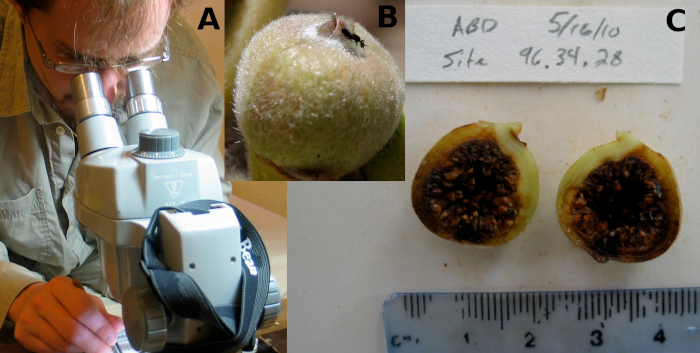
\includegraphics[width=1\linewidth]{img/fig_data_set} \caption{Three images showing the process of collecting data for the dimensions of figs from trees of the Sonoran Desert Rock Fig in Baja, Mexico. (A) Processing fig fruits, which included measuring the diameter of figs along three diferent axes of length, width, and height, (B) a fig still attached to a tree with a fig wasp on top of it, and (C) a sliced open fig with seeds along the inside of it.}\label{fig:unnamed-chunk-23}
\end{figure}

This lab will use the \href{https://raw.githubusercontent.com/bradduthie/statistical_techniques/main/data/soil_organic_carbon.csv}{soil organic carbon} dataset in \protect\hyperlink{02_summary_statistics}{Exercise 8.1} for summary statistics.
The \href{https://raw.githubusercontent.com/bradduthie/statistical_techniques/main/data/fig_fruits.csv}{fig fruits} will be used for \protect\hyperlink{02_transforming_variables}{Exercise 8.2} on transforming variables and \protect\hyperlink{02_computing_variables}{Exercise 8.3} on computing a variable.
Some of these exercises will be similar to what we did in the week 1 practical from \protect\hyperlink{ux5cux23Chapter_3}{Chapter 3}, but in Jamovi rather than a separate spreadsheet.

\hypertarget{summary_statistics_02}{%
\section{Exercise for summary statistics}\label{summary_statistics_02}}

Download the \href{https://raw.githubusercontent.com/bradduthie/SCIU4T4/main/data/soil_organic_carbon.csv}{soil organic carbon} dataset if you have not already done so (right click and ``Save Link As\ldots{}''), and save it in a location where you know you will be able to find it again, then open Jamovi.
Once Jamovi is open, you can import the dataset by clicking on the three horizontal lines in the upper left corner of the tool bar, then selecting `Open' (Figure 8.2).

\begin{figure}
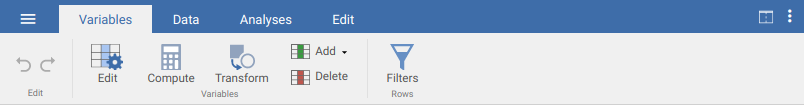
\includegraphics[width=1\linewidth]{img/jamovi_toolbar} \caption{The Jamovi toolbar including tabs for opening files, Variables, Data, Analyses, and Edit. To open a file, select the three horizontal lines in the upper right}\label{fig:unnamed-chunk-25}
\end{figure}

You might need to click `Browse' in the upper right of Jamovi to find the file.
Figure 8.3 below shows how this will look when you browse for a data file.

\begin{figure}
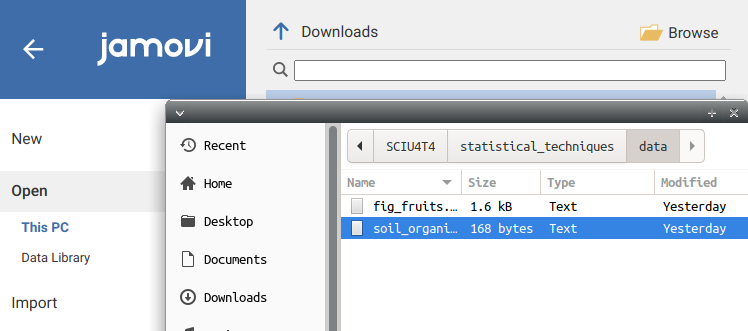
\includegraphics[width=1\linewidth]{img/open_soil_organic_carbon} \caption{The Jamovi interface for opening a file with the 'Import' tab selected. Options for browsing to a file on the computer are available in the upper right, which opens the window in the foreground.}\label{fig:unnamed-chunk-26}
\end{figure}

Once the data are imported, you should see two separate columns.
The first column will show soil organic carbon values for topsoil samples, and the second column will show soil organic carbon values for subsoil samples.
These data are not formatted in a tidy way.
We need to fix this so that each row is a unique observation and each column is a variable (see \protect\hyperlink{Chapter_2}{Chapter 2}).
It might be easiest to reorganise the data in a spreadsheet such as LibreOffice Calc or Microsoft Excel.
But you can also edit the data directly in Jamovi by clicking on the `Data' tab in the toolbar (see Figures 8.2 and 8.4).
The best way to reorganise the data in Jamovi is to double-click on the third column of data next to `subsoil' (see Figure 8.4).

\begin{figure}
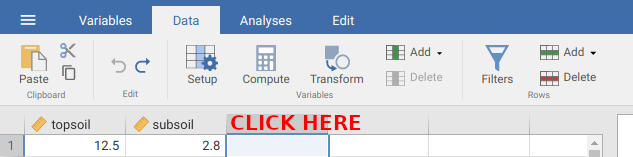
\includegraphics[width=1\linewidth]{img/jamovi_new_variable} \caption{The Jamovi toolbar is shown with the soil organic carbon dataset. In Jamovi, double-clicking above column three where it says 'CLICK HERE' will allow you to input a new variable.}\label{fig:unnamed-chunk-27}
\end{figure}

After double-clicking on the location shown in Figure 8.4, there will be three buttons visible.
You can click the `New Data Variable' to insert a new variable named `soil\_type' in place of the default name `C'.
Keep the `Measure type' as `Nominal', but change the `Data type' to `text'.
When you are done, click the \texttt{\textgreater{}} character to the right so that the variable is fixed (Figure 8.5).

\begin{figure}
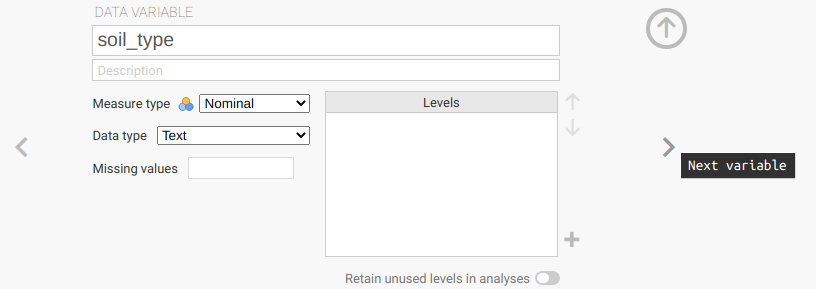
\includegraphics[width=1\linewidth]{img/jamovi_set_variable} \caption{The Jamovi toolbar is shown with the input for creating a new data variable. The new variable added is to indicate the soil type (topsoil or subsoil), so it needs to be a nominal variable with a data type of text.}\label{fig:unnamed-chunk-28}
\end{figure}

After typing in the new variable `soil\_type', add another variable called `organic\_carbon'.
The organic\_carbon variable should have a measure type of `Continuous' and a data type of `Decimal'.
After both soil\_type and organic\_carbon variables have been set, you can click the up arrow with the upper right circle (Figure 8.5) to get the new variable window out of the way.

With the two new variables created, we can now rearrange the data in a tidy way.
The first 19 rows of soil\_type should be `topsoil', and the remaining 15 rows should be `subsoil'.
To do this quickly, you can write `topsoil' in the first row of soil\_type and copy-paste into the remaining rows.
You can do the same to write `subsoil' in the remaining rows 20-34.
Next, copy all of the topsoil values in column 1 into the first 19 rows of column 4, and copy all of the subsoil values in column 2 into the next 15 rows.
After doing all of this, your column 3 (soil\_type) should have the word `topsoil' in rows 1-19 and `subsoil' in rows 20-34.
The values from columns 1 and 2 should now fill rows 1-34 of column 4.
You can now delete the first column of data by right clicking on the column name `topsoil' and selecting `Delete Variable'.
Do the same for the second column `subsoil'.
Now you should have a tidy data set with two columns of data, one called `soil\_type' and one called `organic\_carbon'.
You are now ready to calculate some descriptive statistics from the data.

First, we can calculate the minimum, maximum, and mean of all of the organic carbon values (i.e., the `grand' mean, which includes both soil types).
To do this, select the `Analyses' tab, then click on the left-most button called `Exploration' in the toolbar (Figure 8.6).

\begin{figure}
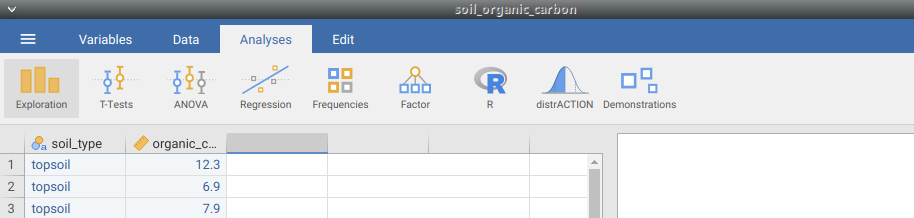
\includegraphics[width=1\linewidth]{img/jamovi_exploration} \caption{The Jamovi toolbar where the tab 'Analyses' can be selected at the very top. Below this tab, the button 'Exploration' can be clicked to calculate descriptive statistics.}\label{fig:unnamed-chunk-29}
\end{figure}

After clicking on `Exploration', a pull-down box will appear with an option for `Descriptives'.
Select this option, and you will see a new window with our two columns of data in the left-most box.
Click once on the `organic\_carbon' variable and use the right arrow to move it into the `Variables' box.
In the right-most panel of Jamovi, a table called `Descriptives' will appear, which will include values for the organic carbon mean, minimum, and maximum.
Write these values on the lines below, and remember to include units.

Grand Mean: \_\_\_\_\_\_\_\_\_\_\_\_\_\_\_\_\_\_\_\_\_\_\_\_\_\_\_\_

Grand Minimum: \_\_\_\_\_\_\_\_\_\_\_\_\_\_\_\_\_\_\_\_\_\_\_\_\_\_\_\_

Grand Maximum: \_\_\_\_\_\_\_\_\_\_\_\_\_\_\_\_\_\_\_\_\_\_\_\_\_\_\_\_

These values might be useful, but recall that there are two different soil types that need to be considered, topsoil and subsoil.
The mean, minimum, and maximum above pools both of these soil types together, but we might instead want to know the mean, minimum, and maximum values for topsoil and subsoil separately.
Splitting organic carbon by soil types is straightforward in Jamovi.
To do it, go back to the Exploration \(\to\) Descriptives option and again put `organic\_carbon' in the Variables box.
This time, however, notice the `Split by' box below the Variables box.
Now, click on `soil\_type' in the descriptives and click on the lower right arrow to move soil type into the `Split by' box.
The table of descriptives in the right window will now break down all of the summary statistics by soil type.
First, write the mean, minimum, and maximum topsoil values below.

Topsoil Mean: \_\_\_\_\_\_\_\_\_\_\_\_\_\_\_\_\_\_\_\_\_\_\_\_\_\_\_\_

Topsoil Minimum: \_\_\_\_\_\_\_\_\_\_\_\_\_\_\_\_\_\_\_\_\_\_\_\_\_\_\_\_

Topsoil Maximum: \_\_\_\_\_\_\_\_\_\_\_\_\_\_\_\_\_\_\_\_\_\_\_\_\_\_\_\_

Next, do the same for the mean, minimum, and maximum subsoil values.

Subsoil Mean: \_\_\_\_\_\_\_\_\_\_\_\_\_\_\_\_\_\_\_\_\_\_\_\_\_\_\_\_

Subsoil Minimum: \_\_\_\_\_\_\_\_\_\_\_\_\_\_\_\_\_\_\_\_\_\_\_\_\_\_\_\_

Subsoil Maximum: \_\_\_\_\_\_\_\_\_\_\_\_\_\_\_\_\_\_\_\_\_\_\_\_\_\_\_\_

From the values above, the mean of organic carbon sampled from the topsoil appears to be greater than the mean of organic carbon sampled from the subsoil.
Assuming that Jamovi has calculated the means correctly, we can be confident that the topsoil \emph{sample} mean is higher.
But what about the \emph{population} means?
Think back to concepts of populations versus samples from \protect\hyperlink{Chapter_4}{Chapter 4}.
Based on these samples in the dataset, can we really say for certain that the population mean of topsoil is higher than the population mean of subsoil?
Think about this, then write a sentence below about how confident we can be about concluding that topsoil organic carbon is greater than subsoil organic carbon.

\begin{verbatim}




\end{verbatim}

What would make you more (or less) confident that topsoil and subsoil population means are different?
Think about this, then write another sentence below that answers the question.

\begin{verbatim}




\end{verbatim}

Note that there is no right or wrong answer for the above two questions.
The entire point of the questions is to help you reflect on your own learning and better link the concepts of populations and samples to the real dataset in this practical.
Doing this will make the statistical hypothesis testing that comes later in the module more clear.

\hypertarget{transforming_variables_02}{%
\section{Exercise on transforming variables}\label{transforming_variables_02}}

In this next exercise, we will work with the \href{https://raw.githubusercontent.com/bradduthie/SCIU4T4/main/data/fig_fruits.csv}{fig fruits} dataset (right click and ``Save Link As\ldots{}'').
Open this dataset into Jamovi.
Note that there are 5 columns of data, and all of the data appear to be in a tidy format.
Each row represents a separate fig fruit, while each column represents a measured variable associated with the fruit.
The first several rows should look like the below.

\begin{verbatim}
##   Tree Length_cm Width_cm Height_cm Seeds
## 1    A       1.5      1.8       1.4   238
## 2    A       1.7      1.9       1.5   198
## 3    A       2.1      2.1       1.6   220
## 4    A       1.5      1.6       1.4   188
## 5    A       1.6      1.6       1.5   139
## 6    A       1.5      1.4       1.5   173
\end{verbatim}

The dataset includes the tree from which the fig was sampled in column 1 (A, B, C, and D), then the length, width, and heights of the fig in cm.
Finally, the last column shows how many seeds were counted within the fig.
Use the Descriptives option in Jamovi to find the grand (i.e., not split by Tree) mean length, width, and height of figs in the dataset.
Write these means down below (remember the units).

Grand Mean length: \_\_\_\_\_\_\_\_\_\_\_\_\_\_\_\_\_\_\_\_\_\_\_\_\_\_\_\_

Grand Mean height: \_\_\_\_\_\_\_\_\_\_\_\_\_\_\_\_\_\_\_\_\_\_\_\_\_\_\_\_

Grand Mean width: \_\_\_\_\_\_\_\_\_\_\_\_\_\_\_\_\_\_\_\_\_\_\_\_\_\_\_\_

Now look at the different rows in the Descriptives table of Jamovi.
Note that there is a row for `Missing', and there appears to be one missing value for fig width and fig height.
This is very common in real datasets.
Sometimes practical limitations in the field prevent data from being collected, or something happens that causes data to be lost.
We therefore need to be able to work with datasets that have missing data.
For now, we will just note the missing data and find them in the actual data set.
Go back to the `Data' tab in Jamovi and find the figs with a missing width and height value.
Report the rows of these missing values below.

Missing width row: \_\_\_\_\_\_\_\_\_\_\_\_\_\_\_\_\_\_\_\_\_\_\_\_\_\_\_\_

Missing height row: \_\_\_\_\_\_\_\_\_\_\_\_\_\_\_\_\_\_\_\_\_\_\_\_\_\_\_\_

Next, we will go back to working with the actual data.
Note that the length, width, and height variables are all recorded in cm to a single decimal place.
Suppose we want to transform these variables so that they are represented in mm instead of cm.
We will start by creating a new column `Length\_mm' by transforming the existing `Length\_cm' column.
To do this, click on the `Data' tab at the top of the toolbar again, then click on the `Length\_cm' column name to highlight the entire column.
Your screen should look like the image in Figure 8.7.

\begin{figure}
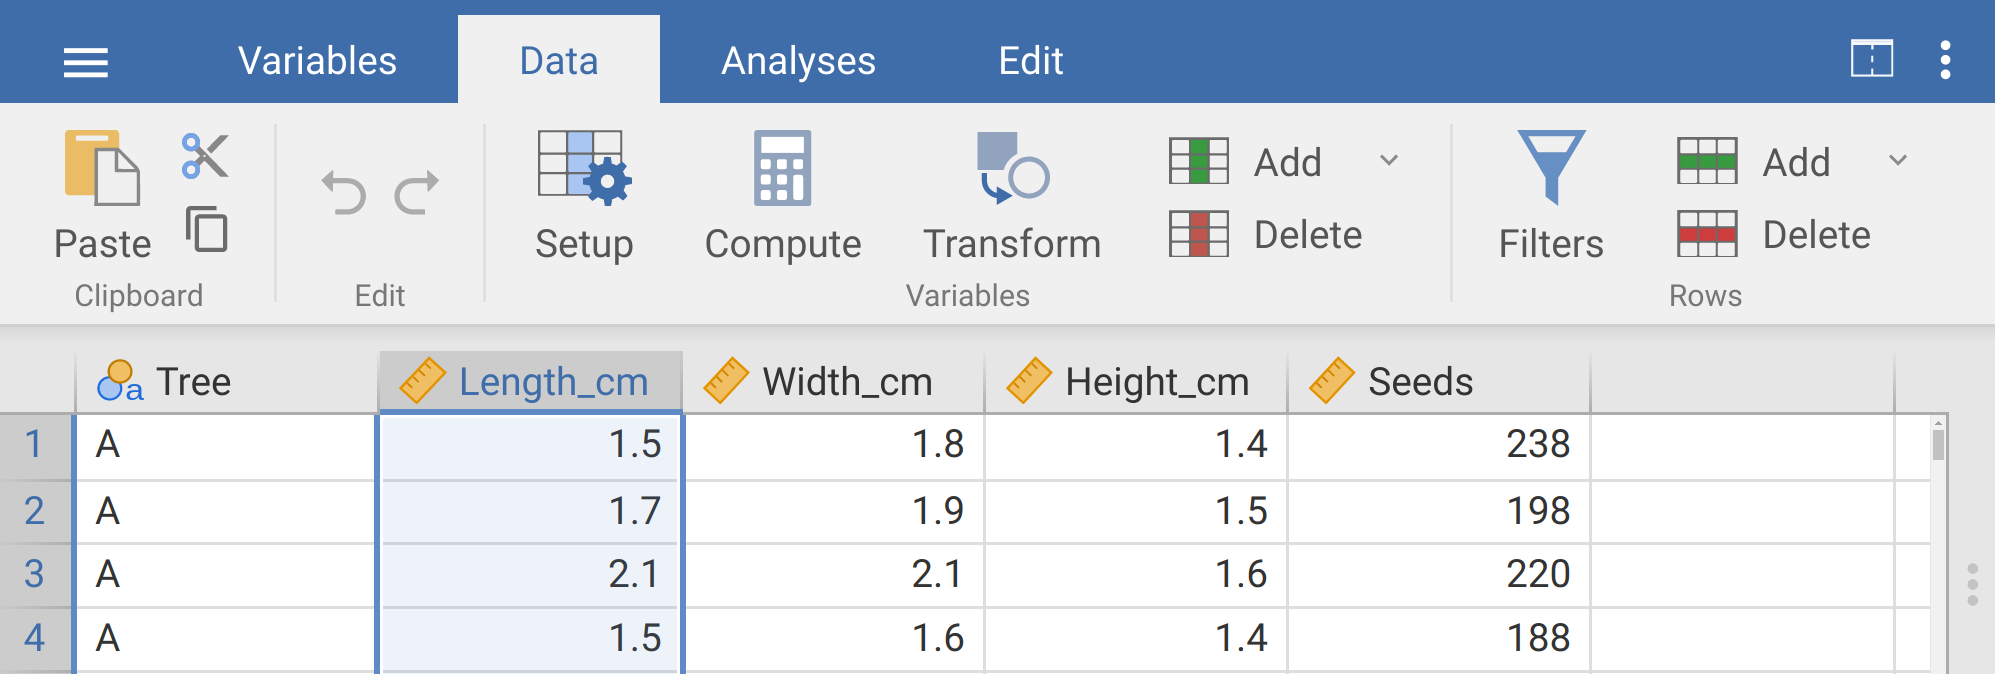
\includegraphics[width=1\linewidth]{img/jamovi_transform_fig_length} \caption{The Jamovi toolbar where the tab 'Data' is selected. The length (cm) column is highlighted and will be transformed by clicking on the Transform button in the toolbar above}\label{fig:unnamed-chunk-31}
\end{figure}

With the `Length\_cm' column highlighted, click on the `Transform' button in the toolbar.
Two things happen next.
First, a new column appears in the dataset that looks identical to `Length\_cm'; ignore this for now.
Second, a box appears below the toolbar allowing us to type in a new name for the transformed variable.
We can call this variable `Length\_mm'.
Below, note the first pulldown menu `Source variable'.
The source value should be `Length\_cm', so we can leave this alone.
The second pulldown menu `using transform' will need to change.
To change the transform from `None', click the arrow and select `Create New Transform' from the pulldown.
A new box will pop up allowing us to name the transformation.
It does not matter what we call it (e.g., `cm\_to\_mm' is fine).
Note that there are 10 mm in 1 cm, so to convert from cm to mm, we need to multiply the values of `Length\_cm' by 10.
We can do this by appending a \texttt{*\ 10} to the lower box of the transform window, so that it reads \texttt{=\ \$source\ *\ 10} (Figure 8.8).

\begin{figure}
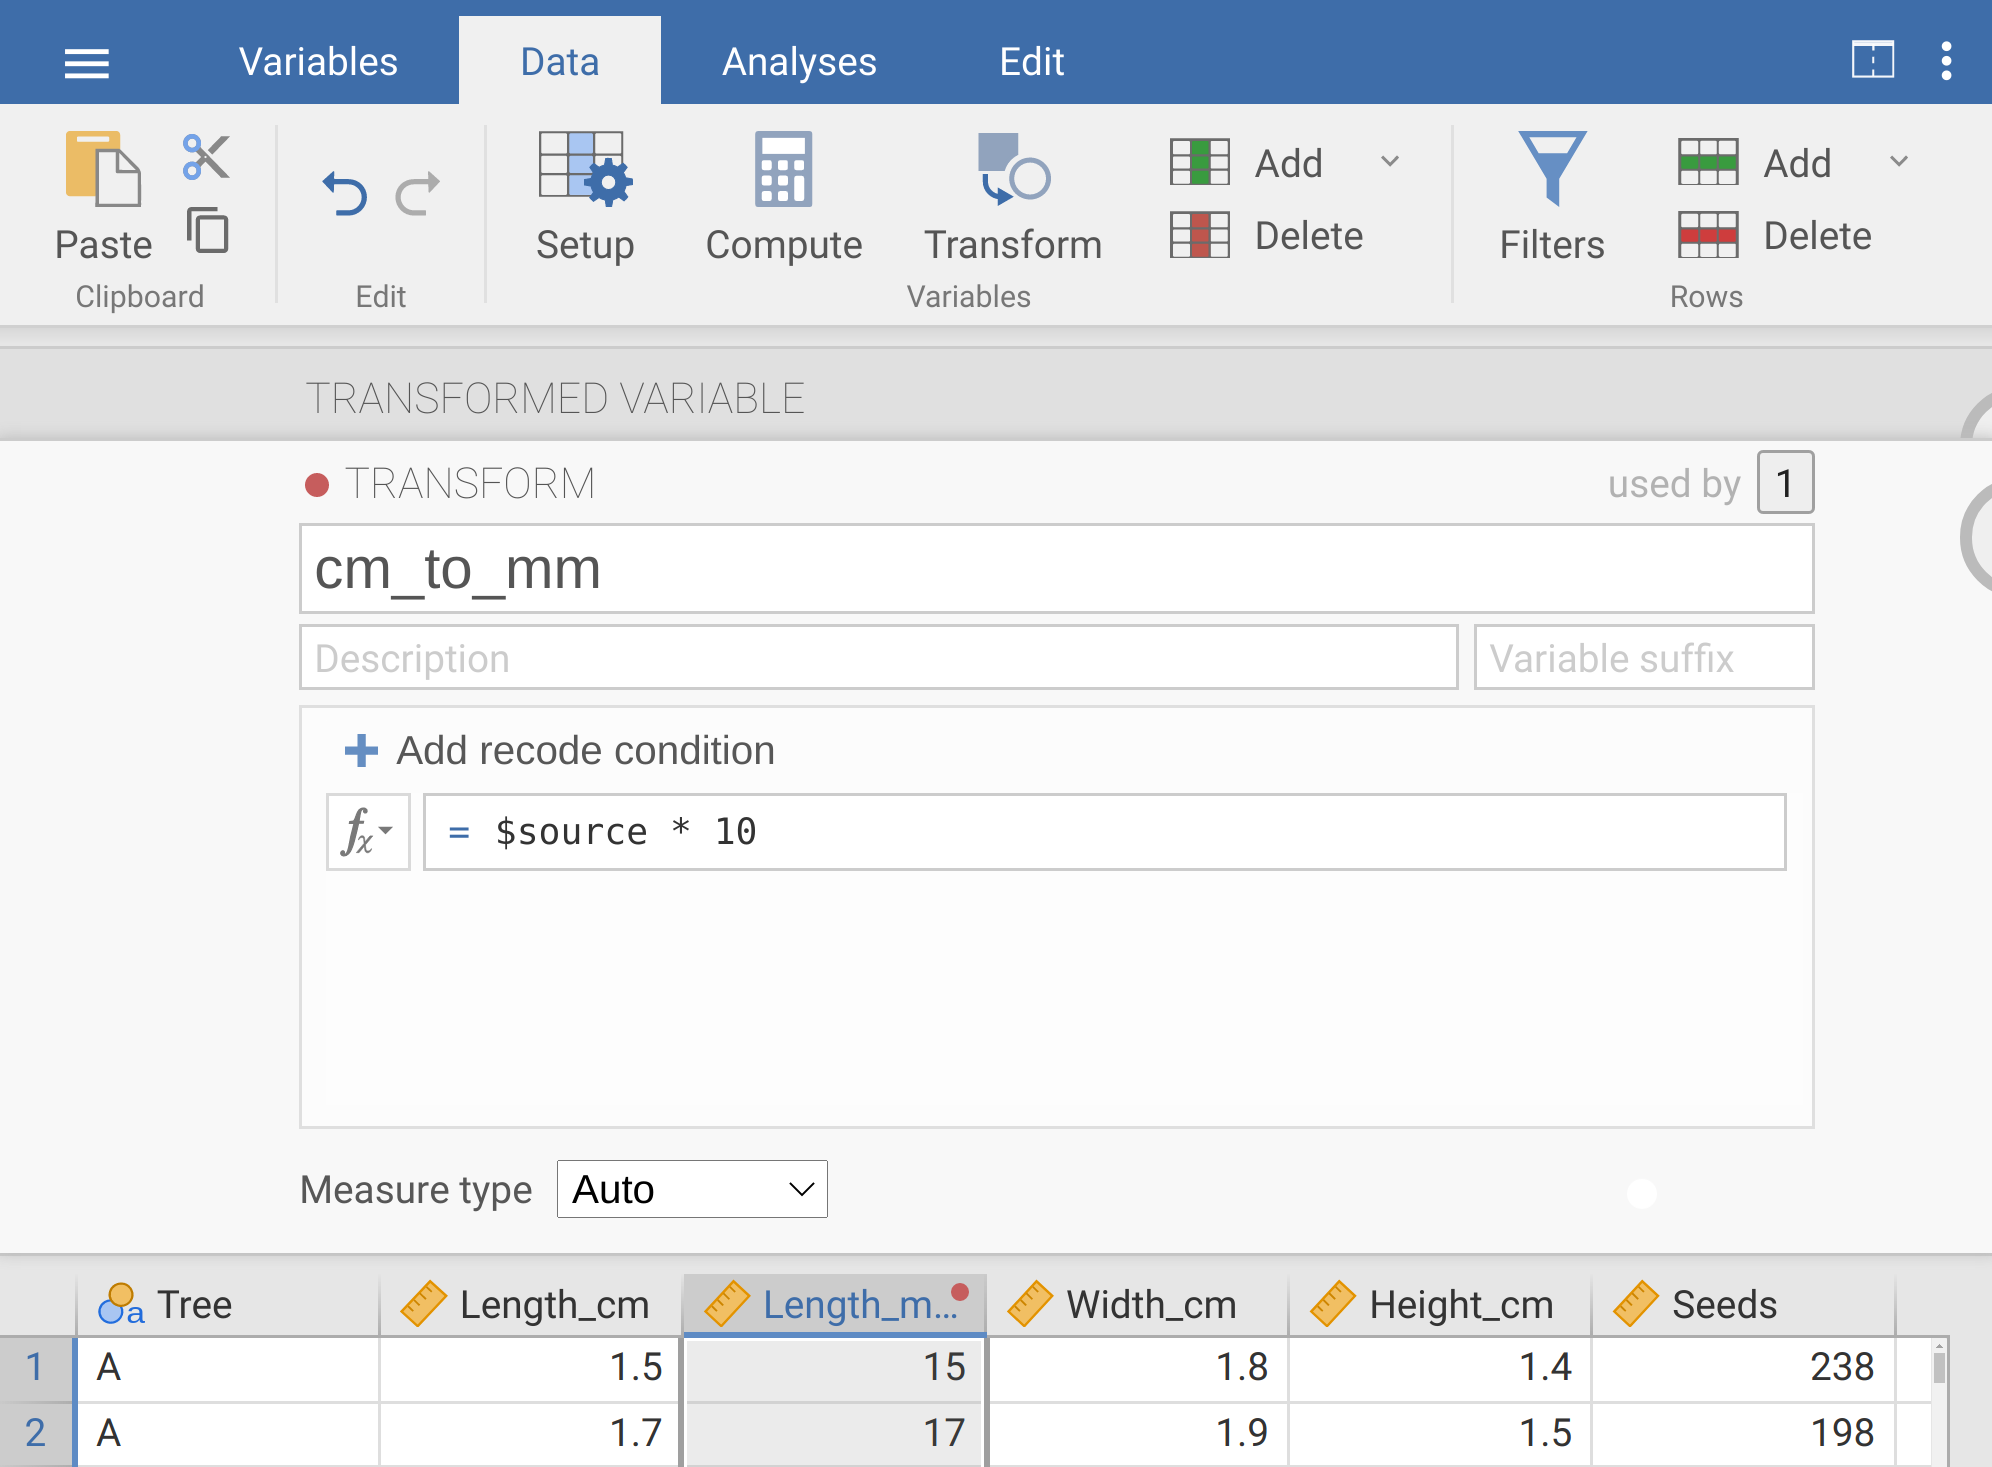
\includegraphics[width=1\linewidth]{img/jamovi_transform_cm_to_mm} \caption{The Jamovi toolbar where the tab 'Data' is selected. The box below shows the transform, which has been named 'cm to mm'. The transformation occurs by multiplying the source (Length mm) by 10. The dataset underneath shows the first few rows with the transformed column highlighted (note that the new 'Length mm' column is 10 times the length column.}\label{fig:unnamed-chunk-32}
\end{figure}

When we are finished, we can click the down arrow inside the circle in the upper right to get rid of the transform window, then the up arrow inside the circle in the upper right to get rid of the transformed variable window.
Now we have a new column called `Length\_mm', in which values are 10 times greater than they are in the adjacent `Length\_cm' column, and therefore represent fig length in mm.
If we want to, we can always change the transformation by double-clicking the `Length\_mm' column.
For now, apply the same transformation to fig width and height, so we have three new columns of length, width, and height all measured in mm (note, if you want to, you can use the saved transformation `cm\_to\_mm' that you used to transform length, saving some time).
At the end of this, you should have eight columns of data, including three new columns that you just created by transforming the existing columns of Length\_cm, Width\_cm, and Height\_cm into the new columns Length\_mm, Width\_mm, and Height\_mm.
Find the means of these three new columns and write them below.

Grand Mean length (mm): \_\_\_\_\_\_\_\_\_\_\_\_\_\_\_\_\_\_\_\_\_\_\_\_\_\_\_\_

Grand Mean height (mm): \_\_\_\_\_\_\_\_\_\_\_\_\_\_\_\_\_\_\_\_\_\_\_\_\_\_\_\_

Grand Mean width (mm): \_\_\_\_\_\_\_\_\_\_\_\_\_\_\_\_\_\_\_\_\_\_\_\_\_\_\_\_

Compare these means to the means calculated above in cm.
Do the differences between means in cm and the means in mm make sense?

\hypertarget{computing_variables_02}{%
\section{Exercise on computing variables}\label{computing_variables_02}}

In this last exercise, we will compute a new variable `fig\_volume'.
Because of the way that the dimensions of the fig were measured in the field, we need to make some simplifying assumptions when calculating volume.
We will assume that fig fruits are perfect spheres, and that the radius of each fig is half of its measured width (i.e., `Width\_mm / 2').
This is obviously not ideal, but sometimes practical limitations in the field make it necessary to make these kinds of simplifying assumptions.
In this case, how might assuming that figs are perfectly spherical affect the accuracy of our estimated fig volume?
Write a sentence of reflection on this question below, drawing from what you have learned this week about accuracy and precision of measurements.

\begin{verbatim}




\end{verbatim}

Now we are ready to make our calculation of fig volume.
The formula for the volume of a sphere (\(V\)) given its radius \(r\) is,

\[V = \frac{4}{3} \pi r^{3}.\]

In words, sphere volume equals four thirds times \(\pi\), times \(r\) cubed (i.e., \(r\) to the third power).
If this equation is confusing, remember that \(\pi\) is approximately 3.14, and taking \(r\) to the third power means that we are multiplying \(r\) by itself 3 times.
We could therefore rewrite the equation above,

\[V = \frac{4}{3} \times 3.14 \times r \times r \times r.\]

This is the formula that we can use to create our new column of data for fig volume.
To do this, double-click on the first empty column of the dataset, just to the right of the `Seeds' column header.
You will see a pull down option in Jamovi with 3 options, one of which is `NEW COMPUTED VARIABLE'.
This is the option that we want.
We need to name this new variable, so we can call it `fig\_volume'.
Next, we need to type in the formula for calculating volume.
First, in the small box next to the \(f_{x}\), type in the (4/3) multiplied by 3.14 as below.

\begin{verbatim}
= (4/3) * 3.14 *
\end{verbatim}

Next, we need to multiply by the variable `Width\_mm' divided by 2 (to get the radius), three times. We can do this by clicking on the \(f_{x}\) box to the left.
Two new boxes will appear; the first is named `Functions', and the second is named `Variables'.
Ignore the functions box for now, and find `Width\_mm' in the list of variables.
Double click on this to put it into the formula, then divide it by 2.
You can repeat this two more times to complete the computed variable as shown in Figure 8.9.

\begin{figure}
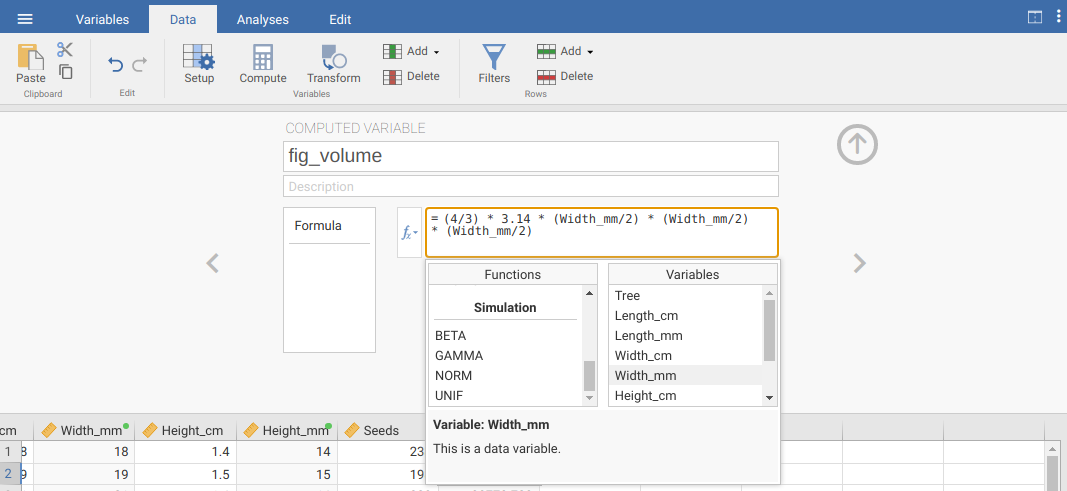
\includegraphics[width=1\linewidth]{img/jamovi_compute_new_variable} \caption{The Jamovi toolbar where the tab 'Data' is selected. The box below shows the new computed variable 'fig volume', which has been created by calculating the product of 4/3, 3.14, and Width mm three times.}\label{fig:unnamed-chunk-33}
\end{figure}

Note that we can get the cube of `Width\_mm' more concisely by using the carrot character (\texttt{\^{}}).
That is, we would get the same answer shown in Figure 8.9 if we instead typed the below in the function box.

\begin{verbatim}
= (4/3) * 3.14 * (Width_mm/2)^3
\end{verbatim}

Note that the order of operations is important here, which is why there are parentheses around \texttt{Width\_mm/2}. This calculation needs to be done before taking the value to the power of 3. If we instead had written, \texttt{Width\_mm/2\^{}3}, then Jamovi would first take the cube of 2 \((2 \times 2 \times 2 = 8)\), then divided \texttt{Width\_mm} by this value giving a different and incorrect answer. When in doubt, it is always useful to use parentheses to specify what calculations should be done first.

You now have the new column of data `fig\_volume'.
Remember that the calculations underlying apply to the units too.
The width of the fig was calculated in mm, but we have taken width to the power of 3 when calculating the volume.
In the spaces below, find the mean, minimum, and maximum volumes of all figs and report them in the correct units.

Mean: \_\_\_\_\_\_\_\_\_\_\_\_\_\_\_\_\_\_\_\_\_\_\_\_\_\_\_\_

Minimum: \_\_\_\_\_\_\_\_\_\_\_\_\_\_\_\_\_\_\_\_\_\_\_\_\_\_\_\_

Maximum: \_\_\_\_\_\_\_\_\_\_\_\_\_\_\_\_\_\_\_\_\_\_\_\_\_\_\_\_

Finally, it would be good to plot these newly calculated fig volume data.
These data are continuous, so we can use a histogram to visualise the fig volume distribution.
To make a histogram, go to the Exploration \(\to\) Descriptives window in Jamovi (the same place where you found the mean, minimum, and maximum).
Now, look on the lower left-hand side of the window and find the pulldown menu for `Plots'.
Click `Plots', and you should see several different plotting options.
Check the option for `Histogram' and see the new histogram plotted in the window to the right.
Draw a rough sketch of the histogram in the area below.

\begin{verbatim}






\end{verbatim}

Finally, we should save the file that we have been working on.
There are two ways to save a file in Jamovi, and it is a good idea to save both ways.
The first way is to use Jamovi's own (binary) file type, which has the extension OMV.
This will not only save the data (including the calculated variables created within Jamovi), but also any analyses that we have done (e.g., calculation of minimums, maximums, and means) or graphs that we have made (e.g., the histogram).
To do this, click on the three horizontal lines in the upper left of the Jamovi toolbar, then select `Save As'.
Choose an appropriate name (e.g., `SCIU4T4\_Week2\_practical.omv'), then save the file in a location where you know that you will be able to find it again.
Like, all binary files, an OMV file cannot be opened as plain text.
Hence, it might be a good idea to save the dataset as a CSV file (note, this will not save any of the analyses or graphs).
To do this, click on the three horizontal lines in the upper left of the toolbar again, but this time click `Export'.
Give the file an appropriate name (e.g., `SCIU4T4\_Week2\_data'), then choose `CSV' from the pulldown menu below (Figure 8.10).

\begin{figure}
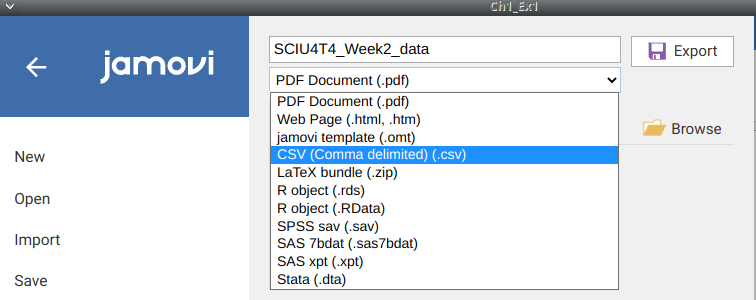
\includegraphics[width=1\linewidth]{img/export_jamovi} \caption{The Jamovi Export menu in which data are be saved as a CSV using the pulldown menu below the filename}\label{fig:unnamed-chunk-34}
\end{figure}

Make sure to choose a save location that you know you will be able to find again (to navigate through file directories, click `Browse' in the upper right).
To save, click on `Export' in the upper right (Figure 8.10).

\hypertarget{summary-1}{%
\section{Summary}\label{summary-1}}

You should now know some of the basic tools for working with data, calculating some simple descriptive statistics, plotting a histogram, and saving output and data in Jamovi.
These skills will be used throughout the module, so it is important to be comfortable with them as the analyses become more complex.
If you still have time at the end of the lab practical, it might be a good idea to explore other features in Jamovi.

\hypertarget{part-summary-statistics}{%
\part{Summary statistics}\label{part-summary-statistics}}

\hypertarget{Week3}{%
\chapter*{Week 3 Overview}\label{Week3}}
\addcontentsline{toc}{chapter}{Week 3 Overview}

\begin{longtable}[]{@{}
  >{\raggedright\arraybackslash}p{(\columnwidth - 2\tabcolsep) * \real{0.3269}}
  >{\raggedright\arraybackslash}p{(\columnwidth - 2\tabcolsep) * \real{0.6731}}@{}}
\toprule
\endhead
\textbf{Dates} & 6 February 2023 - 10 February 2023 \\
\textbf{Reading} & \textbf{Required:} SCIU4T4 Workbook chapters 9-12 \\
& \textbf{Recommended:} \citet{Navarro2022} \href{https://davidfoxcroft.github.io/lsj-book/05-Drawing-graphs.html}{Chapter 5} and \href{https://davidfoxcroft.github.io/lsj-book/04-Descriptive-statistics.html\#measures-of-central-tendency}{Chapter 4.1} \\
& \textbf{Suggested:} \citet{Rowntree2018} Chapter 3 \\
& \textbf{Advanced:} None \\
\textbf{Lectures} & 3.0: Decimal places and significant figures part 1 (7:52 min; \href{https://stirling.cloud.panopto.eu/Panopto/Pages/Viewer.aspx?id=05e7e5ee-65a5-4b78-bd46-af8200d9170b}{Video}) \\
& 3.1: Decimal places and significant figures part 2 (7:08 min; \href{https://stirling.cloud.panopto.eu/Panopto/Pages/Viewer.aspx?id=f4513530-0bd2-4886-8338-af8200d91727}{Video}) \\
& 3.2: Graphs (10:29 min; \href{https://stirling.cloud.panopto.eu/Panopto/Pages/Viewer.aspx?id=35638c1d-0ee7-404d-97fd-af8200d91874}{Video}) \\
& 3.3: Box-whisker plots (8:07 min; \href{https://stirling.cloud.panopto.eu/Panopto/Pages/Viewer.aspx?id=6b8eb060-b936-42ad-a4db-af8200d91892}{Video}) \\
& 3.4: The mean (16:52 min; \href{https://stirling.cloud.panopto.eu/Panopto/Pages/Viewer.aspx?id=f47d8358-b4b6-44ed-8352-af8200d9177c}{Video}) \\
& 3.5: The mode (6:54 min; \href{https://stirling.cloud.panopto.eu/Panopto/Pages/Viewer.aspx?id=999ba5dd-0f42-45f3-9152-af8200d91795}{Video}) \\
& 3.6: The median and quantiles (8:04 min; \href{https://stirling.cloud.panopto.eu/Panopto/Pages/Viewer.aspx?id=72ef44f4-0d1f-4f24-9d96-af8200d917eb}{Video}) \\
& 3.7: Mean, mode, median, and resistance (8:35 min; \href{https://stirling.cloud.panopto.eu/Panopto/Pages/Viewer.aspx?id=a43b6799-040c-4699-9864-af8200d91809}{Video}) \\
& 3.8: The variance (9:40 min; \href{https://stirling.cloud.panopto.eu/Panopto/Pages/Viewer.aspx?id=b7f26e80-a40d-45d4-b4ab-af8200d918fe}{Video}) \\
& 3.9: The standard deviation (6:17 min; \href{https://stirling.cloud.panopto.eu/Panopto/Pages/Viewer.aspx?id=db70798b-16fa-4164-839b-af8200d91919}{Video}) \\
& 3.10: The standard deviation (7:46 min; \href{https://stirling.cloud.panopto.eu/Panopto/Pages/Viewer.aspx?id=9aec6aa5-9e3a-40f6-92f4-af8200d91979}{Video}) \\
& 3.11: The standard deviation (13:23 min; \href{https://stirling.cloud.panopto.eu/Panopto/Pages/Viewer.aspx?id=9c7a11df-7182-4f69-b986-af8200d91994}{Video}) \\
\textbf{Practical} & Plotting and statistical summaries (\protect\hyperlink{Chapter_13}{Chapter 13}) \\
& Room: Cottrell 2A17 \\
& Group A: 08 FEB 2023 (WED) 13:05-15:55 \\
& Group B: 09 FEB 2023 (THU) 09:05-11:55 \\
\textbf{Help hours} & Ian Jones \\
& Room: Cottrell 1A13 \\
& 10 FEB 2023 (FRI) 15:05-17:55 \\
\textbf{Assessments} & \href{https://canvas.stir.ac.uk/courses/13075/quizzes/29674}{Week 3 Practice quiz} on Canvas \\
\bottomrule
\end{longtable}

Week 3 focuses on descriptive statistics, how to report them, interpret them, and communicate them with graphs.

\protect\hyperlink{Chapter_9}{Chapter 9} focuses on how to report numbers with accuracy and precision.
In practice, this means reporting values with the correct number of digits (decimal places and significant figures), and rounding appropriately.

\protect\hyperlink{Chapter_10}{Chapter 10} introduces different types of graphs for communicating data visually.
The chapter focuses specifically on histograms, pie charts, barplots, and box-whisker plots.

\protect\hyperlink{Chapter_11}{Chapter 11} introduces measures of central tendency.
These are measures that describe the centre of the data using a single number.
Measures of central tendency in this chapter include the mean, the mode, the median, and quantiles.

\protect\hyperlink{Chapter_12}{Chapter 12} introduces on measures of spread.
In contrast to measures of central tendency, which focus on the centre of a dataset, measures of spread focus on how much the data are spread out.
Measures of spread in this chapter in clude the range, the inter-quartile range, the variance, the standard deviation, the coefficient of variation, and the standard error.

\protect\hyperlink{Chapter_13}{Chapter 13} guides you through the week 3 practical.
The aim of this practical is to learn how to use Jamovi to generate plots introduced in \protect\hyperlink{Chapter_10}{Chapter 10}, and to find measures of central tendency and spread introduced in \protect\hyperlink{Chapter_11}{Chapter 11} and \protect\hyperlink{Chapter_12}{Chapter 12}, respectively, and report them accurately using the knowledge from \protect\hyperlink{Chapter_9}{Chapter 9}.

\hypertarget{Chapter_9}{%
\chapter{Decimal places, significant figures, and rounding}\label{Chapter_9}}

When making calculations, it is important that any numbers reported are communicated with \protect\hyperlink{Chapter_6}{accuracy and precision}.
This means reporting numbers with the correct number of digits.
This chapter focuses on correctly interpreting the decimal places and significant figures of a number, and correctly rounding.
In your assessments, you will frequently be asked to report an answer to a specific number of decimal places or significant figures, and you will be expected to round numbers correctly.

\hypertarget{decimal-places-and-significant-figures}{%
\section{Decimal places and significant figures}\label{decimal-places-and-significant-figures}}

A higher number of digits communicates a greater level of accuracy.
For example, the number 2.718 expresses a higher precision than 2.7 does.
Reporting 2.718 implies that we know the value is somewhere between 2.7175 and 2.1785, but reporting 2.7 only implies that we know the value is somewhere between 2.65 and 2.75 \citep{Sokal1995}.
These numbers therefore have a different number of \emph{decimal places} and a different number of \emph{significant figures}.
Decimal places and significant figures are related, but not the same.

\textbf{Decimal places} are conceptually easier to understand. These are just the number of digits to the right of the decimal point. For example, 2.718 has 3 decimal places, and 2.7 has 1 decimal place.

\textbf{Significant figures} are a bit more challenging.
These are the number of digits that you need to infer the accuracy of a value.
For example, the number 2.718 has 4 significant figures and 2.7 has 2 significant figures. This sounds straightforward, but it can get confusing when numbers start or end with zeros.
For example, the number 0.045 has only 2 significant figures because the first two zeros only serve as placeholders (note that if this were a measurement of 0.045 m, then we could express the exact same value as 45 mm, so the zeros are not really necessary to indicate measurement accuracy).
In contrast, the measurement 0.045000 has 5 significant figures because the last 3 zeros indicate a higher degree of accuracy than just 0.045 would (i.e., we know the value is somewhere between 0.44995 and 0.45005, not just 0.0445 and 0.0455).
Lastly, the measurement 4500 has only 2 significant figures because the last 2 zeros are only serving as a placeholder to indicate magnitude, not accuracy (if we wanted to represent 4500 with 4 significant figures, we could use scientific notation and express it as \(4.500 \times 10^3\)).

Here is a table with some examples of numbers, their decimal places, and their significant figures.

\begin{longtable}[]{@{}lll@{}}
\caption{Numbers are presented in rows of the first column. Decimal places and significant figures for each row number are presented in the second and third column, respectively.}\tabularnewline
\toprule
Number & Decimal places & Significant figures \\
\midrule
\endfirsthead
\toprule
Number & Decimal places & Significant figures \\
\midrule
\endhead
3.14159 & 5 & 6 \\
0.0333 & 4 & 3 \\
1250 & 0 & 3 \\
50000.0 & 1 & 6 \\
0.12 & 2 & 2 \\
1000000 & 0 & 1 \\
\bottomrule
\end{longtable}

It is a good idea to double-check that the values in these tables make sense.
For assessments, make sure that you are confident that you can report your answer to a given number of decimal places or significant figures.

\hypertarget{rounding}{%
\section{Rounding}\label{rounding}}

Often if you are asked to report a number to a specific number of decimals or significant figures, you will need to round the number.
Rounding reduces the number of significant digits in a number, which might be necessary if a number that we calculate has more significant digits than we are justified in expressing.
There are different rules for rounding numbers, but in this module, we will follow \citet{Sokal1995}.
When rounding to the nearest decimal, the last decimal written should not be changed if the number that immediately follows is 0, 1, 2, 3, or 4.
If the number that immediately follows is 5, 6, 7, 8, or 9, then the last decimal written should be increased by 1.

For example, if we wanted to round the number 3.141593 to 2 significant digits, then we would write it as 3.1 because the digit that immediately follows (i.e., the third digit) is 4.
If we wanted to round the number to 5 significant digits, then we would write it as 3.1416 because the digit that immediately follows is 9.
And if we wanted to round 3.141593 to 4 significant digits, then we would write it as 3.142 because the digit that immediately follows is 5.
Note that this does not just apply for decimals.
If we wanted to round 1253 to 3 significant figures, then we would round by writing it as 1250.

Here is a table with some examples of numbers rounded to a given significant figure.

\begin{longtable}[]{@{}lll@{}}
\caption{Numbers to be rounded are presented in rows of the first column. The significant figures to which rounding is desired is in the second column, and the third column shows the correctly rounded number.}\tabularnewline
\toprule
Original number & Significant figures & Rounded number \\
\midrule
\endfirsthead
\toprule
Original number & Significant figures & Rounded number \\
\midrule
\endhead
23.2439 & 4 & 23.24 \\
10.235 & 4 & 10.24 \\
102.39 & 2 & 100 \\
5.3955 & 3 & 5.40 \\
37.449 & 3 & 37.4 \\
0.00345 & 2 & 0.0035 \\
\bottomrule
\end{longtable}

In this module, it will be necessary to round calculated values to a specified decimal or significant figure.
It is therefore important to understand the rules for rounding and why the values in the table above are rounded correctly.

\hypertarget{Chapter_10}{%
\chapter{Graphs}\label{Chapter_10}}

Graphs are useful tools for visualising and communicating data.
Graphs come in many different types, and different types of graphs are effective for different types of data.
This chapter focuses on 4 types of graphs: (1) histograms, (2) pie charts, (3) barplots, and (4) box-whisker plots.

After collecting or obtaining a new dataset, it is almost always a good idea to plot the data in some way.
Visualisation can often highlight important and obvious properties of a dataset more efficiently that inspecting raw data, calculating summary statistics, or running statistical tests.
When making graphs to communicate data visually, it is important to ensure that the person reading the graph has a clear understanding of what is being presented.
In practice, this means clearly labelling axes with meaningful descriptions and appropriate units, including a descriptive caption, and indicating what any graph symbols mean.
In general, it is also best to make the simplest graph possible for visualising the data, which means avoiding unnecessary colour, three-dimensional display, or unnecessary distractions from the information being conveyed \citep{Dytham2011, Kelleher2011}.
It is also important to ensure that graphs are as accessible as possible, e.g., by providing strong colour contrast and appropriate colour combinations \citep{Elavsky2022}, and alternative text for images where possible.
As a guide, the histogram, pie chart, barplot, and box-whisker plot below illustrate good practice when making graphs.

\hypertarget{histograms}{%
\section{Histograms}\label{histograms}}

Histograms illustrate the distribution of \protect\hyperlink{Chapter_5}{continuous data}.
They are especially useful visualisation tools because it is often important to assess data at a glance and make a decision about how to proceed with a statistical analysis.
The histogram shown in Figure 10.1 provides an example using the \href{https://raw.githubusercontent.com/bradduthie/SCIU4T4/main/data/fig_fruits.csv}{fig fruits} data set from the practical in \protect\hyperlink{Chapter_8}{Chapter 8} (for a step-by-step demonstration of how a histogram is built, see \href{https://bradduthie.shinyapps.io/build_histogram/}{this interactive application}\footnote{Here is the full URL: \url{https://bradduthie.shinyapps.io/build_histogram/}}).

\begin{figure}
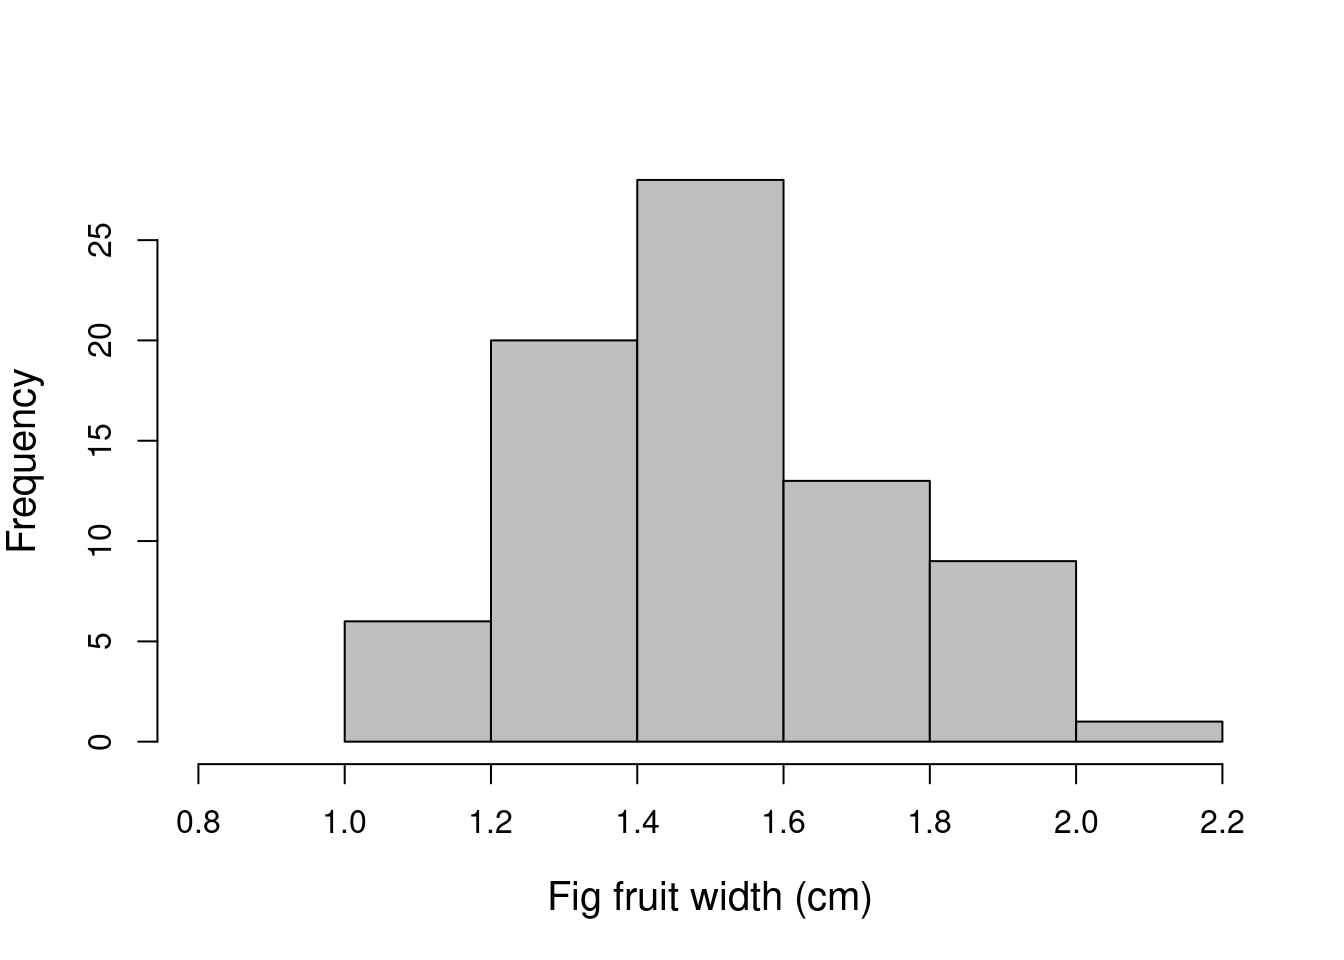
\includegraphics[width=1\linewidth]{bookdown-demo_files/figure-latex/unnamed-chunk-35-1} \caption{Example histogram fig fruit width (cm) using data from 78 fig fruits collected in 2010 from Baja, Mexico.}\label{fig:unnamed-chunk-35}
\end{figure}

The histogram in Figure 10.1 shows how many fruits there are for different intervals of width, i.e., the frequency with which fruits within some width interval occur in the data.
For example, there are 6 fruits with a width between 1.0 and 1.2, so for this interval on the x-axis, the bar is 6 units in height on the y-axis.
In contrast, there is only 1 fig fruit that has a width greater than 2.0 cm (the biggest is 2.1 cm), so we see that the height of the bar for the interval between 2.0 and 2.2 is only 1 unit in frequency.
The bars of the histogram touch each other, which reinforces the idea that the data are \protect\hyperlink{Chapter_5}{continuous} \citep{Dytham2011, Sokal1995}.

\begin{quote}
\href{https://bradduthie.shinyapps.io/build_histogram/}{Click here} for an interactive application showing how histograms are built.
\end{quote}

It is especially important to be able to read and understand information from a histogram because it is often necessary to determine if the data are consistent with the assumptions of a statistical test.
For example, the \emph{shape} of the distribution of fig fruit widths might be important for performing a particular test.
For the purposes of this chapter, the \emph{shape} of the distribution just means what the data look like when plotted like this in a histogram.
In this case, there is a peak toward the centre of the distribution, with fewer low and high values (this kind of distribution is quite common).
Different distribution shapes will be discussed more in \protect\hyperlink{Week4}{Week 4}.

\hypertarget{barplots-and-pie-charts}{%
\section{Barplots and pie charts}\label{barplots-and-pie-charts}}

While histograms are an effective way of visualising \protect\hyperlink{Chapter_5}{continuous data}, barplots (also known as `bar charts' or `bar graphs') and pie charts can be used to visualise \protect\hyperlink{Chapter_5}{categorical data}.
For example, in the \href{https://raw.githubusercontent.com/bradduthie/SCIU4T4/main/data/fig_fruits.csv}{fig fruits} data set from \protect\hyperlink{Chapter_8}{Chapter 8}, 78 fig fruits were collected from 4 different trees (A, B, C, and D).
A barplot could be used to show how many samples were collected from each tree (see Figure 10.2).

\begin{figure}
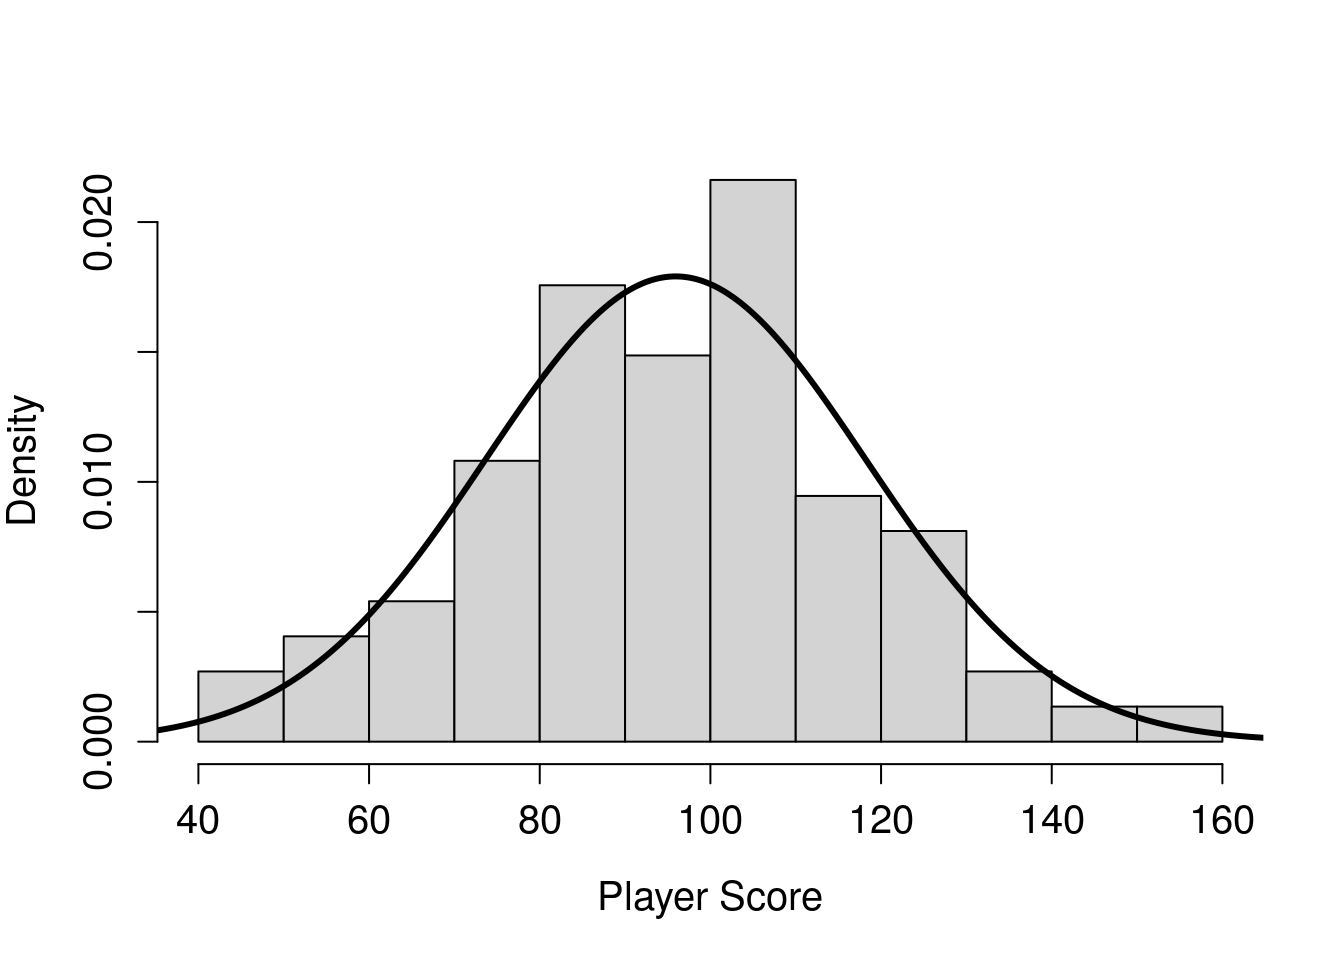
\includegraphics[width=1\linewidth]{bookdown-demo_files/figure-latex/unnamed-chunk-36-1} \caption{Example bar plot showing how many fruits were collected from each of 4 trees (78 collected in total) in 2010 from Baja, Mexico.}\label{fig:unnamed-chunk-36}
\end{figure}

In Figure 10.2, each tree is represented by a separate bar on the x-axis.
Unlike a histogram, the bars do not touch each other, which reinforces the idea that different categories of data are being shown (in this case, different trees).
The height of a bar indicates how many fruits were sampled for each tree.
For example, 14 fruits were sampled from tree A, and 22 fruits were sampled from tree B.
At a glance, it is therefore possible to compare different trees and make inferences about how they differ in sampled fruits.

Pie charts are similar to barplots in that both present categorical data, but pie charts are more effective for visualising the relative quantity for each category.
That is, pie charts illustrate the percentage of measurements for each category.
For example, in the case of the fig fruits, it might be useful to visualise what percentage of fruits were sampled from each tree.
A pie chart could be used to evaluate this, with pie slices corresponding to different trees and the size of each slice reflecting the percentage of the total sampled fruits that came from each tree (Figure 10.3).

\begin{figure}
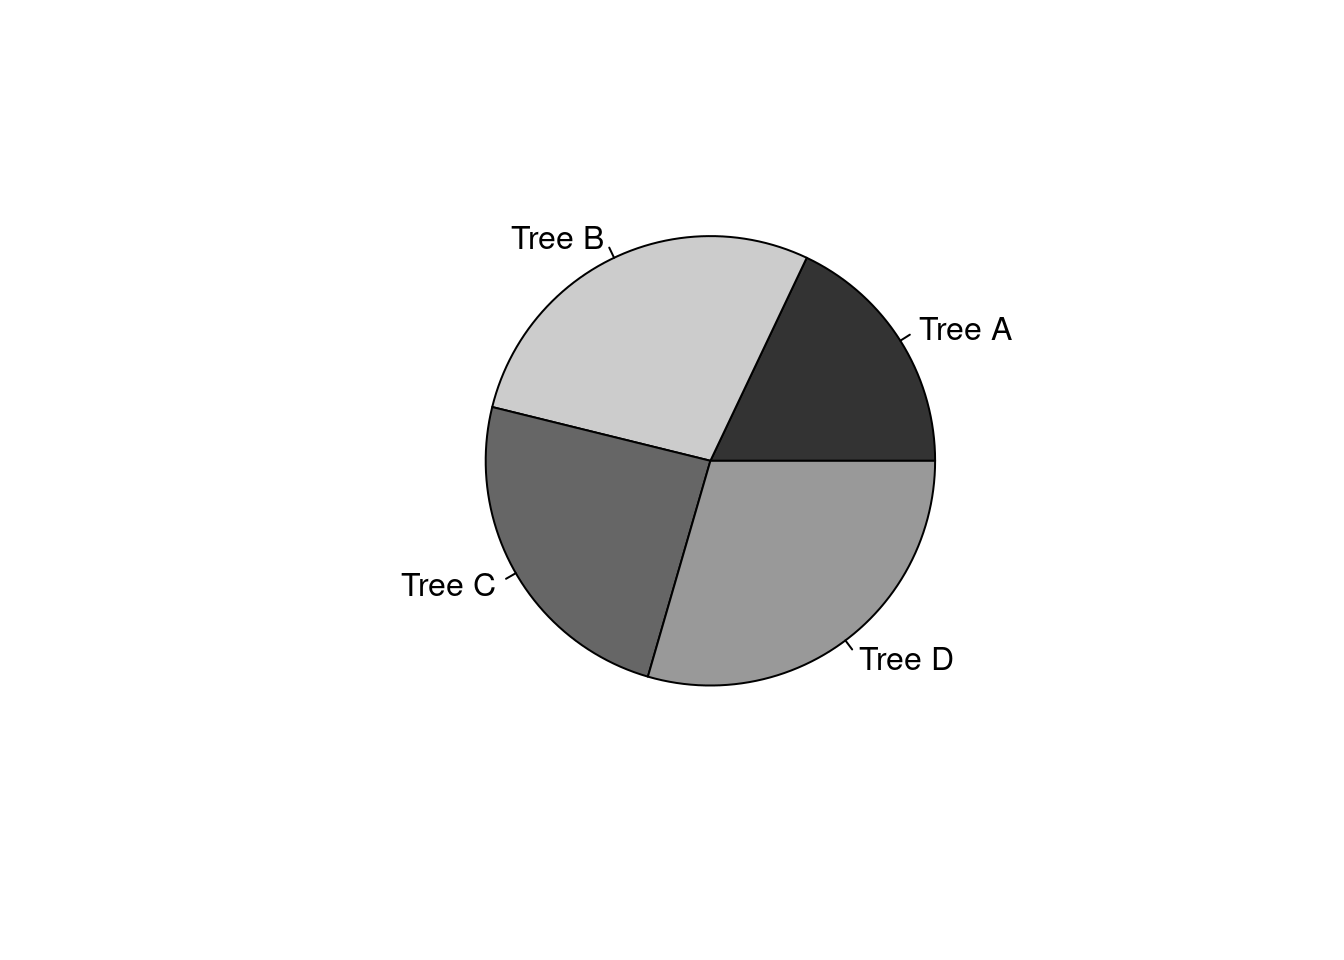
\includegraphics[width=1\linewidth]{bookdown-demo_files/figure-latex/unnamed-chunk-37-1} \caption{Example pie plot showing the percentage of fruits that were collected from each of 4 trees (78 collected in total) in 2010 from Baja, Mexico.}\label{fig:unnamed-chunk-37}
\end{figure}

Pie charts can be useful in some situations, but in the biological and environmental sciences, they are not used as often as barplots.
In contrast to pie charts, barplots present the absolute quantities (in Figure 10.2, e.g., the actual number of fruits sampled per tree), and it is still possible with barplots to infer the percentage each category contributes to the total from the relative sizes of the bars.
Pie charts, in contrast, only illustrate relative percentages unless numbers are used to indicate absolute quantities.
Unless percentage alone is important, barplots are often the preferred way to communicate count data.

\hypertarget{box-whisker-plots}{%
\section{Box-whisker plots}\label{box-whisker-plots}}

Box-whisker plots (also called boxplots) can be used to visualise distributions in a different way than histograms.
Instead of presenting the full distribution, as in a histogram, a box-whisker plot shows where summary statistics are located (summary statistics are explained in \protect\hyperlink{Chapter_11}{Chapter 11} and \protect\hyperlink{Chapter_12}{Chapter 12}).
This allows the distribution of data to be represented in a more compact way, but does not show the full shape of a distribution.
Figure 10.4 compares a box-whisker plot of fig fruit widths (10.4a) with a histogram of fig fruit widths (10.4b).
In other words, both of the panels (`a' and `b') in Figure 10.4 show the same information in two different ways (note that these are the same data as presented in Figure 10.1).

\begin{figure}
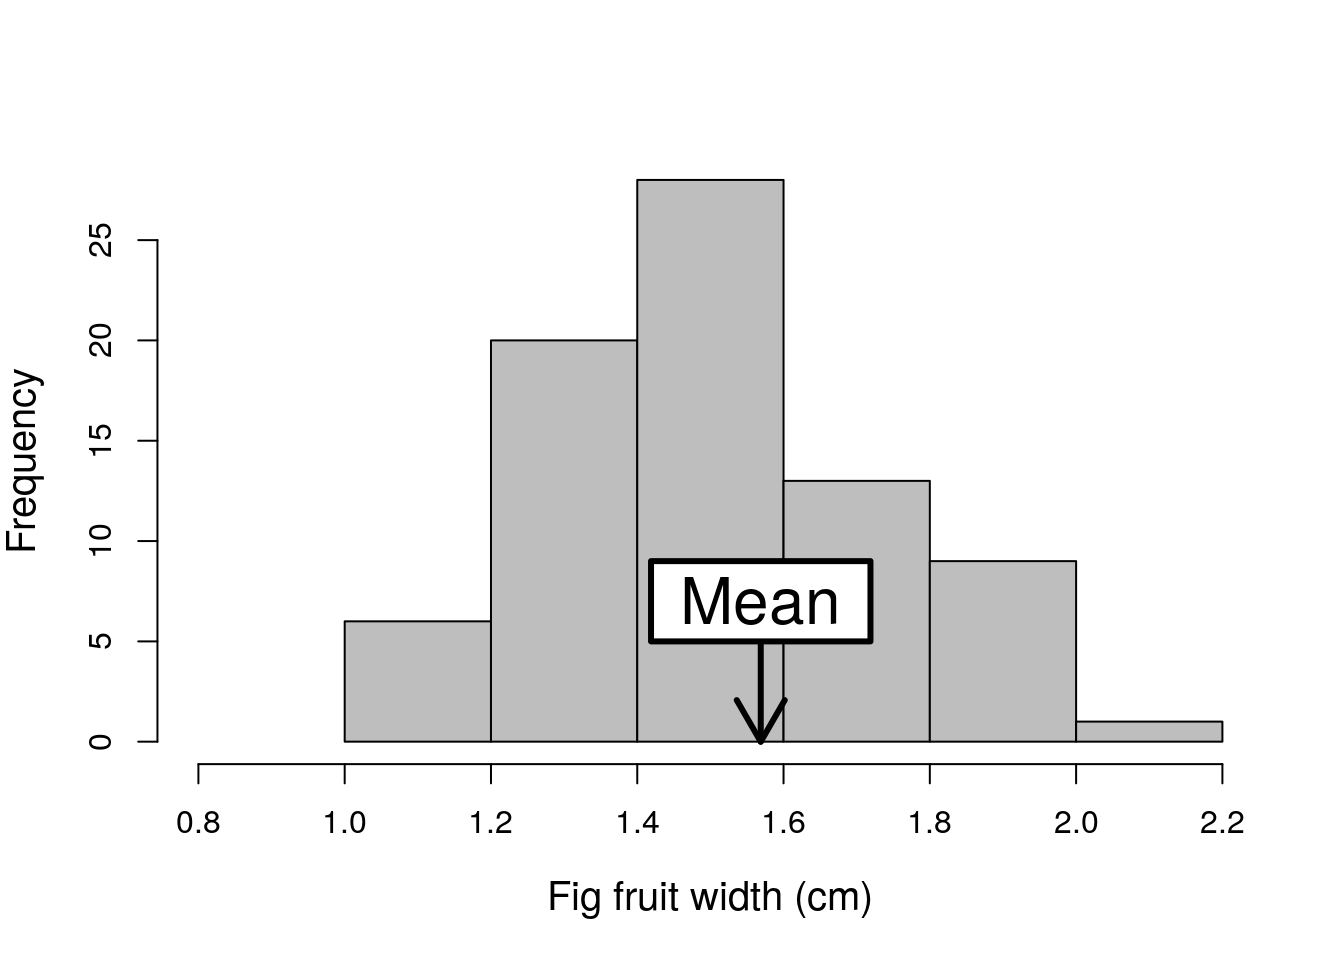
\includegraphics[width=1\linewidth]{bookdown-demo_files/figure-latex/unnamed-chunk-38-1} \caption{Boxplot (a) of fig fruit widths (cm) for 78 fig fruits collected in 2010 in Baja, Mexico. Panel (b) presents the same data as a histogram.}\label{fig:unnamed-chunk-38}
\end{figure}

To show how the panels of Figure 10.4 correspond to one another more clearly, Figure 10.5 shows them again, but with points indicating where the summary statistics shown in the boxplot (Figure 10.5a) are located in the histogram (Figure 10.5b).
These summary statistics include the median (black circles of Figure 10.5), quartiles (red squares of Figure 10.5), and the limits of the distribution (i.e., the minimum and maximum values; blue triangles of Figure 10.5).
Note that in boxplots, if outliers exist, they are presented as separate points.

\begin{figure}
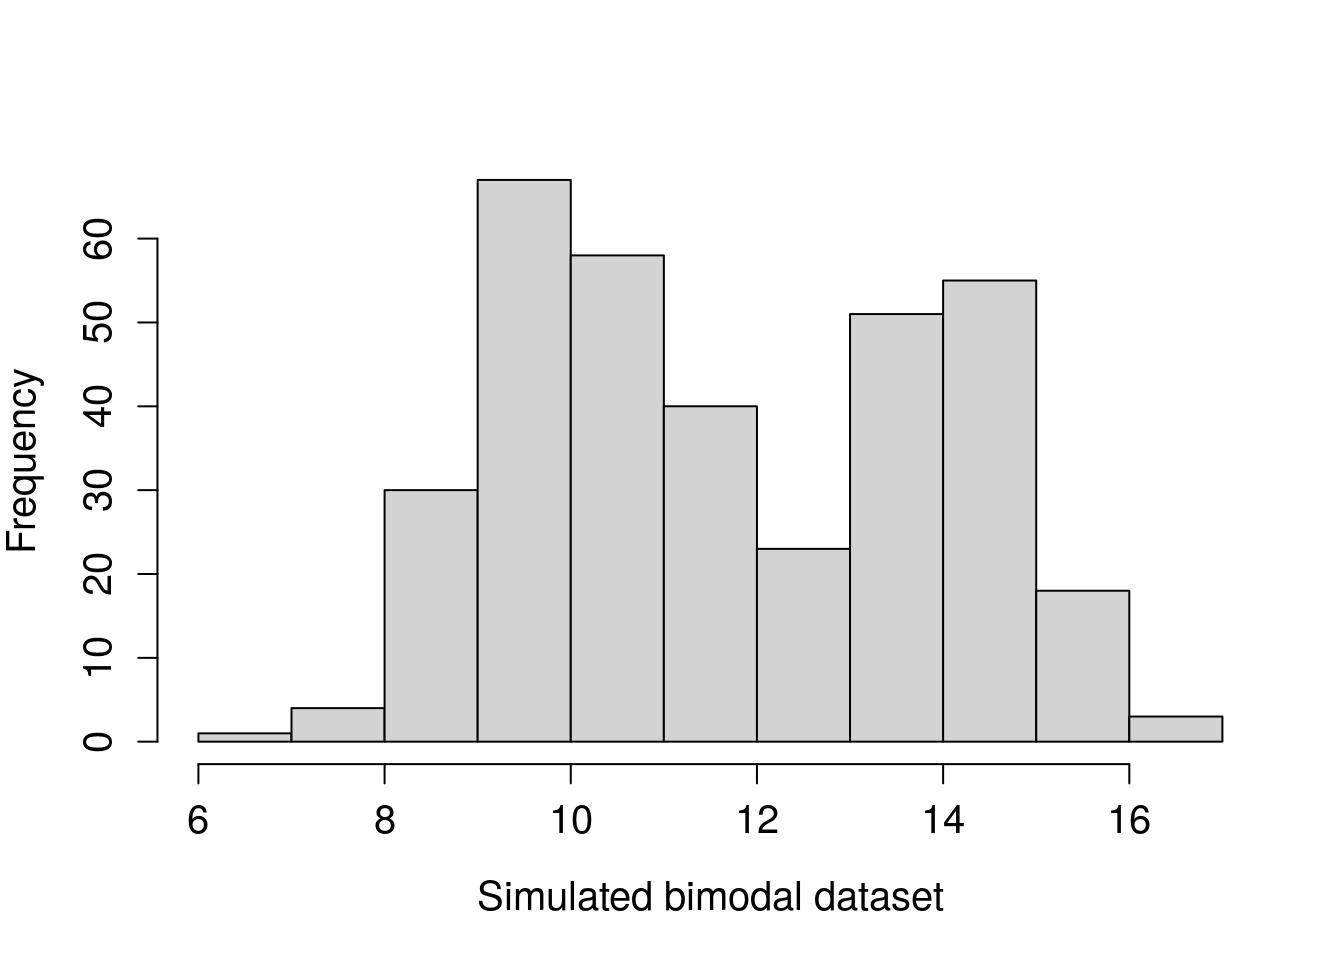
\includegraphics[width=1\linewidth]{bookdown-demo_files/figure-latex/unnamed-chunk-39-1} \caption{Boxplot (a) of fig fruit widths (cm) for 78 fig fruits collected in 2010 in Baja, Mexico. Panel (b) presents the same data as a histogram. Points in the boxplot indicate the median (black circle), first and third quartiles (red squares), and the limits of the distribution (blue triangles). Corresponding locations are shown on the histogram in panel (b).}\label{fig:unnamed-chunk-39}
\end{figure}

One benefit of a boxplot is that it is possible to show the distribution of multiple variables simultaneously.
For example, the distribution of fig fruit width can be shown for each of the four trees side by side on the same x-axis of a boxplot (Figure 10.6).
While it is possible to show histograms side by side, it will quickly take up a lot of space.

\begin{figure}
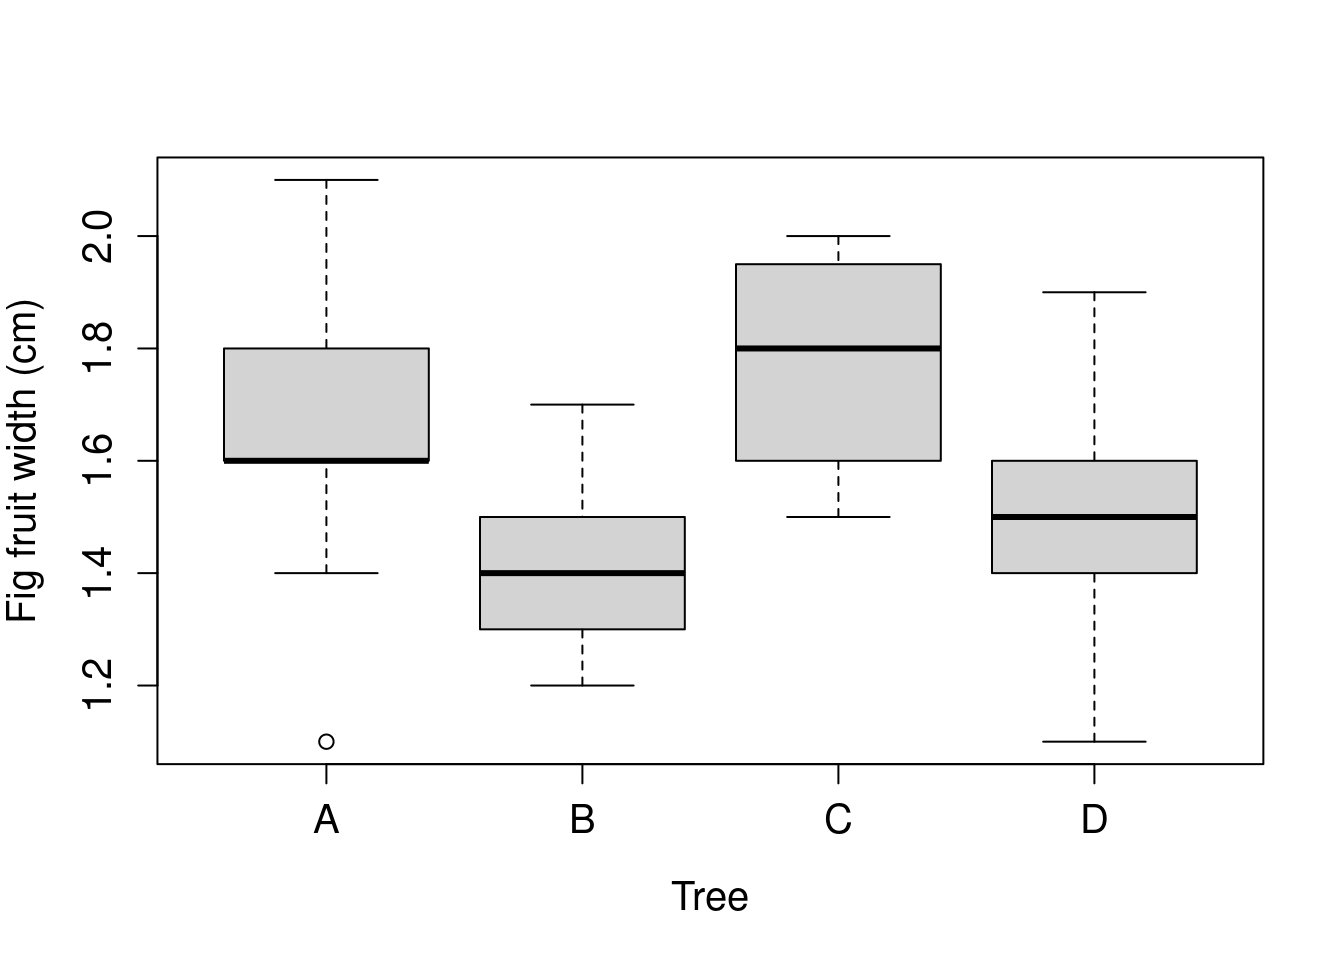
\includegraphics[width=1\linewidth]{bookdown-demo_files/figure-latex/unnamed-chunk-40-1} \caption{Boxplot of fig fruit widths (cm) collected from 4 separate trees sampled in 2010 from Baja, Mexico.}\label{fig:unnamed-chunk-40}
\end{figure}

The boxplot in Figure 10.6 can be used to quickly compare the distribution of Trees A-D.
The point at the bottom of the distribution of Tree A shows an outlier.
This outlier is an especially low value of fig fruit width compared to the other fruits of Tree A.

\hypertarget{Chapter_11}{%
\chapter{Measures of central tendency}\label{Chapter_11}}

Summary statistics describe properties of data in a single number (e.g., the mean), or a set of numbers (e.g., quartiles).
This chapter focuses on summary statistics that describe the centre of a distribution.
It also introduces quantiles, which divide a distribution into different percentages of the data (e.g., the lowest 50\% or highest 75\%).
Throughout this section, verbal and mathematical explanations of summary statistics will be presented alongside histograms or boxplots that convey the same information.
The point of doing this is to help connect the two ways of summarising the data.
All of the summary statistics that follow describe calculations for a \emph{sample} and are therefore estimates of the true values in a \emph{population}.
Recall from \protect\hyperlink{Chapter_4}{Chapter 4} the difference between a population and a sample.
This module focuses on statistical techniques, not statistical theory, so summary statistics will just focus on how to estimate statistics from sampled data instead of how statistics are defined mathematically\footnote{If interested, a good textbook for learning about theoretical statistics and the mathematics underlying what we do in this module is \citet{Miller2004}.}.

\hypertarget{the-mean}{%
\section{The mean}\label{the-mean}}

The arithmetic mean (hereafter just \emph{the mean}\footnote{There are other types of means, such as the geometric mean or the harmonic mean, but we will not use these at all in this module.}) of a sample is one of the most commonly reported statistics when communicating information about a dataset.
The mean is a measure of central tendency, so it is located somewhere in the middle of a distribution.
Figure 11.1 shows the same histogram of fig fruit widths shown in Figure 10.1, but with an arrow indicating where the mean of the distribution is located

\begin{figure}
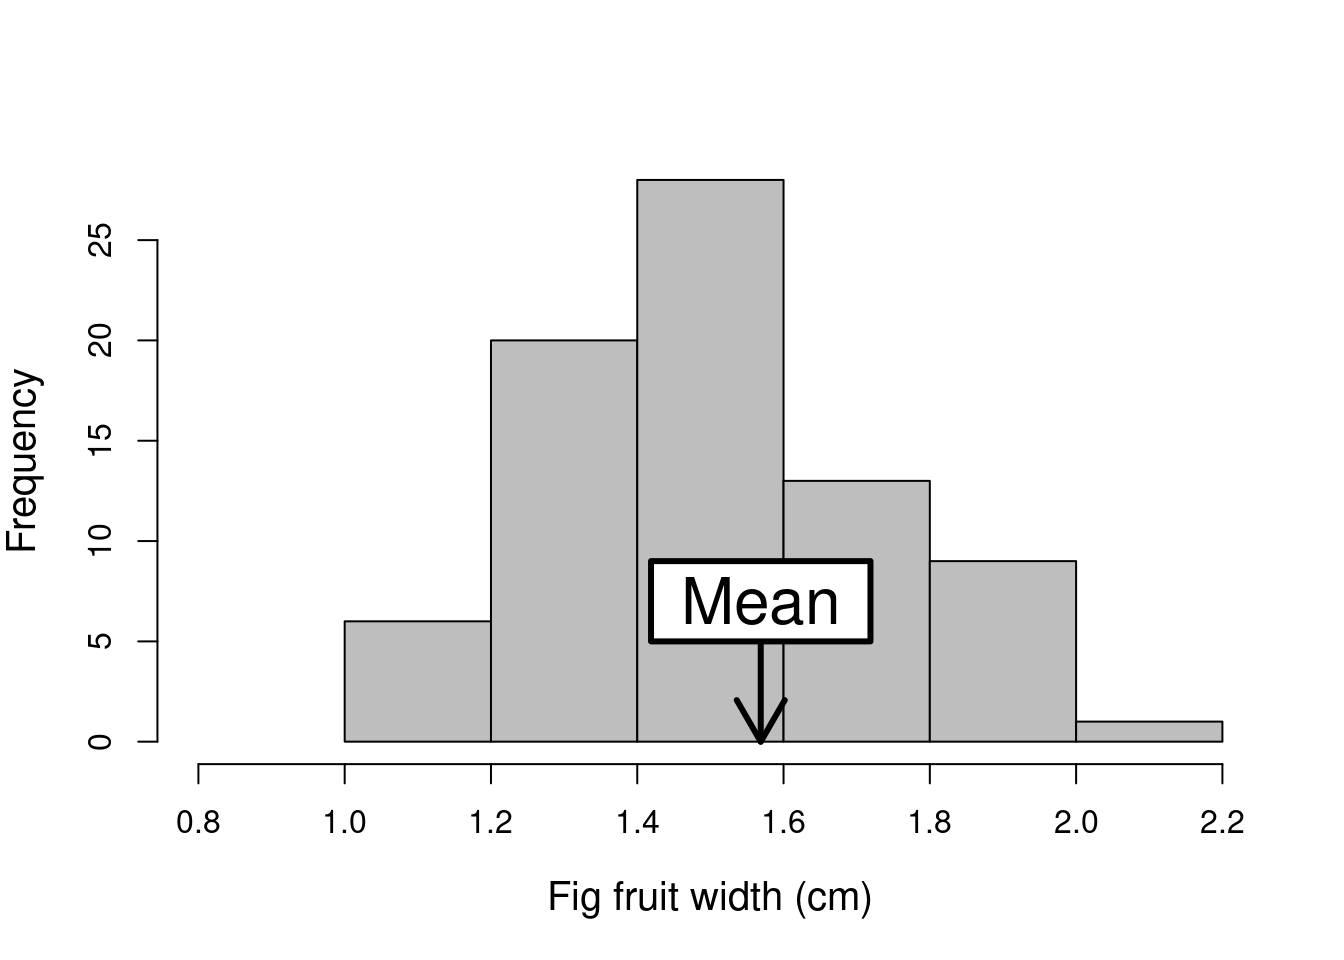
\includegraphics[width=1\linewidth]{bookdown-demo_files/figure-latex/unnamed-chunk-41-1} \caption{Example histogram fig fruit width (cm) using data from 78 fig fruits collected in 2010 from Baja, Mexico. The mean of the distribution is indicated with an arrow.}\label{fig:unnamed-chunk-41}
\end{figure}

The mean is calculated by adding up the values of all of the data and dividing this sum by the total number of data \citep{Sokal1995}.
This is a fairly straightforward calculation, so we can use the mean as an example to demonstrate some new mathematical notation that will be used throughout the module.
We will start with a concrete example with actual numbers, then end with a more abstract equation describing how any sample mean is calculated.
The notation might be a bit confusing at first, but learning it will make understanding statistical concepts easier later in the module.
There are a lot of equations in what follows, but this is because we want to explain what is happening as clearly as possible, step by step.
We start with the following 8 values.

\begin{verbatim}
4.2, 5.0, 3.1, 4.2, 3.8, 4.6, 4.0, 3.5
\end{verbatim}

To calculate the mean of a sample, we just need to add up all of the values and divide by 8 (the total number of values),

\[\bar{x} = \frac{4.2 + 5.0 + 3.1 + 4.2 + 3.8 + 4.6 + 4.0 + 3.5}{8}.\]

Note that we have used the symbol \(\bar{x}\) to represent the mean of \(x\), which is a common notation \citep{Sokal1995}.
In the example above, \(\bar{x} = 4.05\).

Writing the full calculation above is not a problem because we only have 8 points of data.
But sample sizes are often much larger than 8.
If we had a sample size of 80 or 800, then there is no way that we could write down every number to show how the mean is calculated.
One way to get around this is to use ellipses and just show the first and last couple of numbers,

\[\bar{x} = \frac{4.2 + 5.0 + ... + 4.0 + 3.5}{8}.\]

This is a more compact, and perfectly acceptable, way to write the sample mean.
But it is often necessary to have an even more compact way of indicating the sum over a set of values (i.e., the top of the fraction above).
To do this, each value can be symbolised by an \(x\), with a unique subscript \(i\), so that \(x_{i}\) corresponds to a specific value in the list above.
The usefulness of this notation, \(x_{i}\), will become clear soon.
It takes some getting used to, but the table below shows each symbol with its corresponding value to make it more intuitive.

\begin{longtable}[]{@{}ll@{}}
\caption{A sample dataset that includes eight values.}\tabularnewline
\toprule
Symbol & Value \\
\midrule
\endfirsthead
\toprule
Symbol & Value \\
\midrule
\endhead
\(x_{1}\) & 4.2 \\
\(x_{2}\) & 5.0 \\
\(x_{3}\) & 3.1 \\
\(x_{4}\) & 4.2 \\
\(x_{5}\) & 3.8 \\
\(x_{6}\) & 4.6 \\
\(x_{7}\) & 4.0 \\
\(x_{8}\) & 3.5 \\
\bottomrule
\end{longtable}

Note that we can first replace the actual values with their corresponding \(x_{i}\), so the mean can be written as,

\[\bar{x} = \frac{x_{1} + x_{2} + x_{3} + x_{4} + x_{5} + x_{6} + x_{7} + x_{8}}{8}.\]
Next, we can rewrite the top of the equation in a different form using a summation sign,

\[\sum_{i = 1}^{8}x_{i} = x_{1} + x_{2} + x_{3} + x_{4} + x_{5} + x_{6} + x_{7} + x_{8}.\]
Like the use of \(x_{i}\), the summation sign \(\sum\) takes some getting used to, but here it just means ``sum up all of the \(x_{i}\) values''.
You can think of it as a big `S' that just says ``sum up''.
The bottom of the S tells you the starting point, and the top of it tells you the ending point, for adding numbers.
Verbally, we can read this as saying, ``starting with \(i = 1\), add up all of the \(x_{i}\) values until \(i = 8\)''.
We can then replace the long list of \(x\) values with a summation,

\[\bar{x} = \frac{\sum_{i = 1}^{8}x_{i}}{8}.\]

This looks a bit messy, so we can rewrite the above equation.
Instead of dividing the summation by 8, we can multiply it by 1/8, which gives us the same answer,

\[\bar{x} = \frac{1}{8}\sum_{i = 1}^{8}x_{i}.\]

There is one more step.
We have started with 8 actual values and ended with a compact and abstract equation for calculating the mean.
But if we want a general description for calculating \emph{any} mean, then we need to account for sample sizes not equal to 8.
To do this, we can use \(N\) to represent the sample size.
In our example, \(N = 8\), but it is possible to have a sample size be any finite value above zero.
We can therefore replace 8 with \(N\) in the equation for the sample mean,

\[\bar{x} = \frac{1}{N}\sum_{i = 1}^{N}x_{i}.\]

There we have it.
Verbally, the above equation tells us to multiply \(1/N\) by the sum of all \(x_{i}\) values from 1 to \(N\).
This describes the mean for any sample that we might collect.

\hypertarget{the-mode}{%
\section{The mode}\label{the-mode}}

The mode of a dataset is simply the value that appears most often.
As a simple example, we can again consider the sample dataset of 8 values.

\begin{verbatim}
4.2, 5.0, 3.1, 4.2, 3.8, 4.6, 4.0, 3.5
\end{verbatim}

In this dataset, the values 5.0, 3.1, 3.8, 4.6, 4.0, and 3.5 are all represented once.
But the value 4.2 appears twice, once in the first position and once in the fourth position.
Because 4.2 appears most frequently in the dataset, it is the mode of the dataset.

Note that it is possible for a dataset to have more than one mode.
Also, somewhat confusingly, distributions that have more than one peak are often described as multimodal, even if the peaks are not of the same height \citep{Sokal1995}.
For example, the histogram in Figure 11.2 might be described as bimodal because it has two distinct peaks (one around 10 and the other around 14), even though these peaks are not the same size.

\begin{figure}
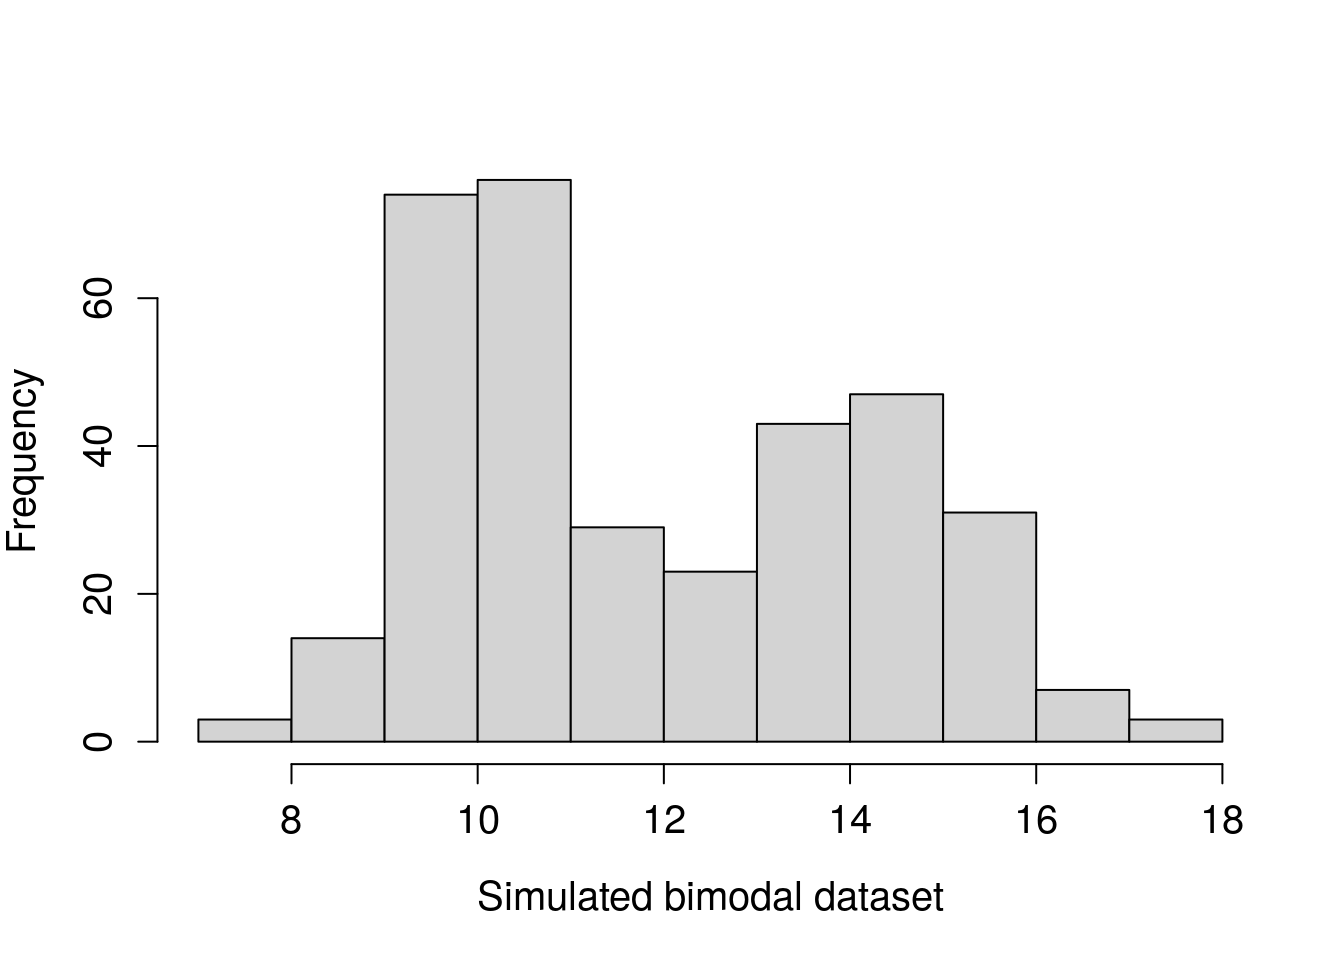
\includegraphics[width=1\linewidth]{bookdown-demo_files/figure-latex/unnamed-chunk-42-1} \caption{Example histogram of a hypothetical dataset that has a bimodal distribution.}\label{fig:unnamed-chunk-42}
\end{figure}

In very rare cases, data might have a U-shape.
The lowest point of the U would then be described as the antimode \citep{Sokal1995}.

\hypertarget{the-median-and-quantiles}{%
\section{The median and quantiles}\label{the-median-and-quantiles}}

The median of a dataset is the middle value when the data are sorted.
More technically, the median is defined as the value that has the same number of lower and higher values than it \citep{Sokal1995}.
If there are an odd number of values in the dataset, then finding the median is often easy.
For example, the median of the values \{8, 5, 3, 2, 6\} is 5.
This is because if we sort the values from lowest to highest (2, 3, 5, 6, 8), the value 5 is exactly in the middle.
It gets more complicated for an even number of values, such as the sample dataset used for explaining the mean and mode.

\begin{verbatim}
4.2, 5.0, 3.1, 4.2, 3.8, 4.6, 4.0, 3.5
\end{verbatim}

We can order these values from lowest to highest.

\begin{verbatim}
3.1, 3.5, 3.8, 4.0, 4.2, 4.2, 4.6, 5.0
\end{verbatim}

Again, there is no middle value here.
But we can find a value that has the same number of lower and higher values.
To do this, we just need to find the mean of the middle 2 numbers, in this case 4.0 and 4.2, which are in positions 4 and 5, respectively.
The mean of 4.0 and 4.2 is, \((4.0 + 4.2)/2 = 4.1\), so 4.1 is the median value.

The median is a type of quantile.
A quantile divides a sorted dataset into different percentages that are lower or higher than it.
Hence, the median could also be called the 50\% quantile because 50\% of values are lower than the median and 50\% of values are higher than it.
Two other quantiles besides the median are also noteworthy.
The first quartile (also called the ``lower quartile'') defines the value for which 25\% of values are lower and 75\% of values are higher.
The third quartile (also called the ``upper quartile'') defines the value for which 75\% of values are lower and 25\% of values are higher.
Sometimes this is easy to calculate.
For example, if there are only five values in a dataset, then the lower quartile is the number in the second position when the data are sorted because 1 value (25\%) is below it and 3 values (75\%) are above it.
For example, for the values \{1, 3, 4, 8, 9\}, the value 3 is the first quartile and 8 is the third quartile.

In some cases, it is not always this clear.
We can show how quantiles get more complicated using the same 8 values as above where the first quartile is somewhere between 3.5 and 3.8.

\begin{verbatim}
3.1, 3.5, 3.8, 4.0, 4.2, 4.2, 4.6, 5.0
\end{verbatim}

There are at least 9 different ways to calculate the first quartile in this case, and different statistical software package will sometimes use different default methods \citep{Hyndman1996}.
One logical way is to calculate the mean between the second (3.5) and third (3.8) position as you would do for the median \citep{Rowntree2018}, \((3.5 + 3.8) / 2 = 3.65\).
Jamovi uses a slightly more complex method, which will give a value of \(3.725\).

It is important to emphasise that no one way of calculating quantiles is the one and only correct way.
Statisticians have just proposed different approaches to calculating quantiles from data, and these different approaches sometimes give slightly different results.
This can be unsatisfying when first learning statistics because it would be nice to have a single approach that is demonstrably correct, i.e., the \emph{right} answer under all circumstances.
Unfortunately, this is not the case here, nor is it the case for a lot of statistical techniques.
Often there are different approaches to answering the same statistical question and no simple right answer.
For this module, we will almost always be reporting calculations of quantiles from Jamovi, and we will clearly indicate that this is how they should be calculated for assessment questions.
But it is important to recognise that different statistical tools might give different answers \citep{Hyndman1996}.

\hypertarget{Chapter_12}{%
\chapter{Measures of spread}\label{Chapter_12}}

It is often important to know how much a set of numbers is spread out.
That is, do all of the data cluster close to the mean, or are most values distant from the mean.
For example, all of the numbers below are quite close to the mean of 5.0 (3 numbers are exactly 5.0).

\begin{verbatim}
4.9, 5.3, 5.0, 4.7, 5.1, 5.0, 5.0
\end{verbatim}

In contrast, all of the numbers that follow are relatively distant from the same mean of 5.0.

\begin{verbatim}
3.0, 5.6, 7.8, 1.2, 4.3, 8.2, 4.9
\end{verbatim}

This chapter focuses on summary statistics that describe the spread of data.
The approach in this chapter is similar to \protect\hyperlink{Chapter_11}{Chapter 11}, which provided verbal and mathematical explanations of measures of central tendency.
We will start with the most intuitive measures of spread, the range and inter-quartile range.
Then, we will move on to some more conceptually challenging measures of spread, the variance, standard deviation, coefficient of variation, and standard error.
These more challenging measures can be a bit confusing at first, but they are absolutely critical for doing statistics.
The best approach to learning them is to see them and practice using them in different contexts, which we will do here, in the \protect\hyperlink{Chapter_13}{Chapter 13} practical, and throughout the semester.

\hypertarget{the-range}{%
\section{The range}\label{the-range}}

The range of a set of numbers is probably the most intuitive measure of spread.
It is simply the difference between the highest and the lowest value of a dataset \citep{Sokal1995}.
To calculate it, we just need to take the highest value minus the lowest value.
If we want to be fancy, then we can write a general equation for the range of a random variable \(X\),

\[Range(X) = \max(X) - \min(X).\]

But really, all that we need to worry about is finding the highest and lowest values, then subtracting.
Consider again the two sets of numbers introduced at the beginning of the chapter.
In examples, it is often helpful to imagine numbers as representing something concrete that has been measured, so suppose that these numbers are the measured masses (in grams) of leaves from two different plants.
Below are the masses of plant A, in which leaf masses are very similar and close to the mean of 5.

\begin{verbatim}
4.9, 5.3, 5.0, 4.7, 5.1, 5.0, 5.0
\end{verbatim}

Plant B masses are below, which are more spread out around the same mean of 5.

\begin{verbatim}
3.0, 5.6, 7.8, 1.2, 4.3, 8.2, 4.9
\end{verbatim}

To get the range of plant A, we just need to find the highest (5.3 g) and lowest (4.7 g) mass, then subtract,

\[Range(Plant\:A) = 5.3 - 4.7 = 0.6\]

Plant A therefore has a range of 0.6 g.
We can do the same for plant B, which has a highest value of 8.2 g and lowest value of 1.2 g,

\[Range(Plant\:B) = 8.2 - 1.2 = 7.0\]

Plant B therefore has a much higher range than plant A.

It is important to mention that the range is highly sensitive to outliers \citep{Navarro2022}.
Just adding a single number to either plant A or plant B could dramatically change the range.
For example, imagine if we measured a leaf in plant A to have a mass of 19.7 g (i.e., we found a huge leaf!).
The range of plant A would then be \(19.7 - 4.7 = 14\) instead of 0.6!
Just this one massive leaf would then make the range of plant A double the range of plant B.
This lack of robustness can really limit how useful the range is as a statistical measure of spread.

\hypertarget{the-inter-quartile-range}{%
\section{The inter-quartile range}\label{the-inter-quartile-range}}

The inter-quartile range (usually abbreviated as `IQR') is conceptually the same as the range.
The only difference is that we are calculating the range between quartiles rather than the range between the highest and lowest numbers in the dataset.
A general formula subtracting the first quartile (\(Q_{1}\)) from the third quartile (\(Q_{3}\)) is,

\[IQR = Q_{3} - Q_{1}.\]

Recall from \protect\hyperlink{Chapter_11}{Chapter 11} how to calculate first and third quartiles.
As a reminder, we can sort the leaf masses for plant A below.

\begin{verbatim}
4.7, 4.9, 5.0, 5.0, 5.0, 5.1, 5.3
\end{verbatim}

The first quartile will be the mean between 4.9 and 5.0 (4.95).
The second quartile will be the the mean between 5.0 and 5.1 (5.05).
The IQR of plant A is therefore,

\[IQR_{plant\:A} = 5.05 - 4.95 = 0.1.\]

We can calculate the IQR for plant B in the same way.
Here are the masses of plant B leaves sorted.

\begin{verbatim}
1.2, 3.0, 4.3, 4.9, 5.6, 7.8, 8.2
\end{verbatim}

The first quartile of plant B is 3.65, and the third quartile is 6.70.
To get the IQR of plant B,

\[IQR_{plant\:B} = 6.70 - 3.65 = 3.05.\]

An important point about the IQR is that it is more robust than the range \citep{Dytham2011}.
Recall that if we found an outlier leaf of 19.7 g on plant A, it would change the range of plant leaf mass from 0.6 g to 14 g.
The IQR is not nearly so sensitive.
If we include the outlier, the first quartile for plant A changes from \(Q_{1} = 4.95\) to \(Q_{1} = 4.975\).
The second quartile changes from \(Q_{3} = 5.05\) to \(Q_{3} = 5.150\).
The resulting IQR is therefore \(5.150 - 4.975 = 0.175\).
Hence, the IQR only changes from 0.1 to 0.175, rather than from 0.6 to 14.
The one outlier therefore has a huge effect on the range, but only a modest effect on the IQR.

\hypertarget{the-variance}{%
\section{The variance}\label{the-variance}}

The range and inter-quartile range were reasonably intuitive, in the sense that it is not too difficult to think about what a range of 10, e.g., actually means in terms of the data.
We now move to measures of spread that are less intuitive.
These measures of spread are the variance, standard deviation, coefficient of variation, and standard error.
These can be confusing and unintuitive at first, but they are extremely useful.
We will start with the variance; this section is long because we want to break the variance down carefully, step by step.

The sample variance of a dataset is a measure of the expected squared distance of data from the mean.
To calculate the variance of a sample, we need to know the sample size (\(N\), i.e., how many measurements in total), and the mean of the sample (\(\bar{x}\)).
We can calculate the variance of a sample (\(s^{2}\)) as follows,

\[s^{2} = \frac{1}{N - 1}\sum_{i = 1}^{N}\left(x_{i} - \bar{x} \right)^{2}.\]

This looks like a lot, but we can break down what the equation is doing verbally.
First, we can look inside the summation (\(\sum\)).
Here we are taking an individual measurement \(x_{i}\), subtracting the mean \(\bar{x}\), then squaring.
We do this for each \(x_{i}\), summing up all of the values from \(i = 1\) to \(i = N\).
This part of the equation is called the \textbf{sum of squares} (\(SS\)),

\[SS = \sum_{i = 1}^{N}\left(x_{i} - \bar{x} \right)^{2}\]

That is, we need to subtract the mean from each value \(x_{i}\), square the result, and add everything up.
Once we have this sum, \(SS\), then we just need to multiply by \(1 / (N - 1)\) to get the variance.

An example of how to do the actual calculation should help make it easier to understand what is going on.
We can use the same values from plant A earlier.

\begin{verbatim}
4.9, 5.3, 5.0, 4.7, 5.1, 5.0, 5.0
\end{verbatim}

To calculate the variance of plant A leaf masses, we start with the sum of squares.
That is, take 4.9, subtract the sample mean of 5.0 (\(4.9 - 5.0 = -0.1\)), then square the result (\((-0.1)^{2} = 0.01\)).
We do the same for 5.3, \((5.3 - 5.0)^{2} = 0.09\), and add it to the 0.01, then continue down the list of numbers finishing with 5.0.
This is what the sum of squares calculation looks like all written out,

\[SS = (4.9 - 5)^{2} + (5.3 - 5)^{2} + (5 - 5)^{2} + (4.7 - 5)^{2} + (5.1 - 5)^{2} + (5 - 5)^{2} + (5 - 5)^{2}.\]

Remember that the calculations in parentheses need to be done first, so the next step for calculating the sum of squares would be the following,

\[SS = (-0.1)^{2} + (0.3)^{2} + (0)^{2} + (-0.3)^{2} + (0.1)^{2} + (0)^{2} + (0)^{2}.\]

Next, we need to square all of the values,

\[SS = 0.01 + 0.09 + 0 + 0.09 + 0.01 + 0 + 0.\]

If we sum the above, we get \(SS = 0.2\).
We now just need to multiply this by \(1 / (N - 1)\), where \(N = 7\) because this is the total number of measurements in the plant A dataset,

\[s^{2} = \frac{1}{7 - 1}\left(0.2\right).\]

From the above, we get a variance of approximately \(s^{2} = 0.0333\).

Fortunately, it will almost never be necessary to calculate a variance manually in this way.
Any statistical software will do all of these steps and calculate the variance for us (\protect\hyperlink{Chapter_13}{Chapter 13} explains how in Jamovi).
The only reason that we present the step-by-step calculation here is to help explain the equation for \(s^{2}\).
The details can be helpful for understanding how the variance works as a measure of spread.
For example, note that what we are really doing here is getting the distance of each value from the mean, \(x_{i} - \bar{x}\).
If these distances tend to be large, then it means that most data points (\(x_{i}\)) are far away from the mean (\(\bar{x}\)), and the variance (\(s^{2}\)) will therefore increase.
The differences \(x_{i} - \bar{x}\) are squared because we need all of the values to be positive, so that variance increases regardless of whether a value \(x_{i}\) is higher or lower than the mean.
It does not matter if \(x_{i}\) is 0.1 lower than \(\bar{x}\) (i.e., \(x_{i} - \bar{x} = -0.1\)), or 0.1 higher (i.e., \(x_{i} - \bar{x} = 0.1\)).
In both cases, the deviation from the mean is the same.
Moreover, if we did not square the values, then the sum of \(x_{i} - \bar{x}\) values would always be 0 (you can try this yourself)\footnote{If you are wondering why we square the difference \(x_{i} - \bar{x}\) instead of just taking its absolute value, this is an excellent question! You have just invented something called the mean absolute deviation. There are some reasons why the mean absolute deviation is not as good of a measure of spread as the variance. \citet{Navarro2022} explain the mean absolute deviation, and how it relates to the variance, very well in \href{https://davidfoxcroft.github.io/lsj-book/04-Descriptive-statistics.html\#mean-absolute-deviation}{section 4.2.3} of their textbook. We will not get into these points here, but it would be good to check out \citet{Navarro2022} for more explanation.}.
Lastly, it turns out that the variance is actually a special case of a more general concept called the \emph{covariance}, which we will look at later in \protect\hyperlink{Week9}{Week 9} and makes the squaring of differences make a bit more sense.

We sum up all of the squared deviations to get the \(SS\), then divide by the sample size minus 1, to get the mean squared deviation from the mean.
That is, the whole process gives us the \emph{average} squared deviation from the mean.
But wait, why is it the sample size minus 1, \(N - 1\)?
Why would we subtract 1 here?
The short answer is that in calculating a \emph{sample} variance, \(s^{2}\), we are almost always trying to estimate the corresponding \emph{population} variance (\(\sigma^{2}\)).
And if we were to just use \(N\) instead of \(N - 1\), then our \(s^{2}\) would be a biased estimate of \(\sigma^{2}\) (see \protect\hyperlink{Chapter_4}{Chapter 4} for a reminder on the difference between samples and populations).
By subtracting 1, we are correcting for this bias to get a more accurate estimate of the population variance.
It is not necessary to do this ourselves; statistical software like Jamovi and R will do it automatically.
This is really all that it is necessary to know for now, but see this footnote\footnote{To get the true population variance \(\sigma^{2}\), we would also need to know the true mean \(\mu\). But we can only estimate \(\mu\) from the sample, \(\bar{x}\). That is, what we would really want to calculate is \(x_{i} - \mu\), but the best we can do is \(x_{i} - \bar{x}\). The consequence of this is that there will be some error that underestimates the true distance of \(x_{i}\) values from the population mean, \(\mu\). Here is the really cool part; to determine the extent to which our estimate of the variance is biased by using \(\bar{x}\) instead of \(\mu\), we just need to know the expected squared difference between the two values, \((\bar{x} - \mu)^{2}\). It turns out that this difference (i.e., the bias of our estimate \(s^{2}\)) is just \(\sigma^{2} / N\); that is, the true variance of the population divided by the sample size. If we subtract this value from \(\sigma^{2}\), so \(\sigma^{2} - \sigma^{2}/N\), then we can get the expected difference between the true variance and the estimate from the sample size. We can rearrange \(\sigma^{2} - \sigma^{2}/N\) to get \(\sigma^{2} \times (N - 1)/N\), which means that we need to correct our sample variance by \(N / (N-1)\) to get an unbiased estimate of \(\sigma^{2}\). If all of this is confusing, that is okay! This is really only relevant for those interested in statistical theory, which is not the focus of this module.} for a bit more detailed explanation to try to make this intuitive (it is actually quite cool!).
Later, we will explore the broader concept of \emph{degrees of freedom}, which explains why we need to take into account the number of parameters in a statistic that are free to vary when calculating a statistic\footnote{Briefly, in the case of sample variance, note that we needed to use all the values \(x_{i}\) in the dataset and the sample mean \(\bar{x}\). But if we know what all of the \(x_{i}\) values are, then we also know \(\bar{x}\). And if we know all but one value of \(x_{i}\) and \(\bar{x}\), then we could figure out the last \(x_{i}\). Hence, while we are using \(N\) values in the calculation of \(s^{2}\), the use of \(\bar{x}\) reduces the degree to which these values are free to vary. We have lost 1 degree of freedom in the calculation of \(\bar{x}\), so we need to account for this in our calculation of \(s^{2}\) by dividing by \(N - 1\). This is another way to think about the \(N - 1\) correction factor \citep{Sokal1995} explained in the previous footnote.}.

This was a lot of information.
The variance is not an intuitive concept.
In addition to being a challenge to calculate, the calculation of a variance leaves us with a value in units squared.
That is, for the example of plant leaf mass in grams, the variance is measured in grams squared, \(g^{2}\), which is not particularly easy to interpret.
For more on this, \citet{Navarro2022} have a really good \href{https://davidfoxcroft.github.io/lsj-book/04-Descriptive-statistics.html\#variance}{section} on the variance.
Despite its challenges as a descriptive statistic, the variance has some mathematical properties that are very useful \citep{Navarro2022}, especially in the biological and environmental sciences.

For example, variances are additive, meaning that if we are measuring two separate characteristics of a sample, A and B, then the variance of A+B equals the variance of A plus the variance of B; i.e., \(Var(A + B) = Var(A) + Var(B)\) \footnote{This has one caveat, which is not important for now. Values of A and B must be uncorrelated. That is, A and B cannot covary. If A and B covary, i.e., \(Cov(A, B) \neq 0\), then \(Var(A+B) = Var(A) + Var(B) + Cov(A, B)\). That is, we need to account for the covariance when calculating \(Var(A+B)\).}.
This is relevant to genetics when measuring heritability.
Here, the total variance in the phenotype of a population (e.g., body mass of animals) can be partitioned into variance attributable to genetics plus variance attributable to the environment,

\[Var(Phenotype) = Var(Genotype) + Var(Environment).\]

This is also sometimes written as \(V_{P} = V_{G} + V_{E}\).
Applying this equation to calculate heritability (\(H^{2} = V_{G} / V_{P}\)) can be used to predict how a population will respond to natural selection.
This is just one place where variance reveals itself to be a highly useful statistic in practice.
Nevertheless, as a descriptive statistic to communicate the spread of a variable, it usually makes more sense to calculate the standard deviation of the mean.

\hypertarget{the-standard-deviation}{%
\section{The standard deviation}\label{the-standard-deviation}}

The standard deviation of the mean (\(s\)) is just the square root of the variance,

\[s = \sqrt{\frac{1}{N - 1}\sum_{i = 1}^{N}\left(x_{i} - \bar{x} \right)^{2}}.\]

This is a simple step, mathematically, but it also is easier to understand conceptually as a measure of spread \citep{Navarro2022}.
By taking the square root of the variance, our units are no longer squared, so we can interpret the standard deviation in the same terms as our original data.
For example, the leaf masses of plant A and plant B in the example above were measured in grams.
While the variance of these masses were in \(g^{2}\), the standard deviation is in \(g\), just like the original measurements.
For plant A, we calculated a leaf mass variance of \(s^{2} = 0.0333\:g^{2}\), which means that the standard deviation of leaf masses is \(s = \sqrt{0.0333\:g^{2}} = 0.1825\:g\).
Because we are reporting \(s\) in the original units, it is a very useful measure of spread to report, and it is an important one to be able to interpret.
To help with the interpretation, here is \href{https://bradduthie.shinyapps.io/forest/}{an interactive tool} showing how the heights of trees in a forest change across different standard deviation values\footnote{Here is the full URL: \url{https://bradduthie.shinyapps.io/forest/}}.

\begin{quote}
\href{https://bradduthie.shinyapps.io/forest/}{Click here} for an interactive application to illustrate the standard deviation.
\end{quote}

Here is another \href{https://bradduthie.shinyapps.io/normal_pos_neg/}{interactive tool} showing how the shape of a histogram changes when the standard deviation of a distribution is changed\footnote{Here is the full URL: \url{https://bradduthie.shinyapps.io/normal_pos_neg/}}.

\begin{quote}
\href{https://bradduthie.shinyapps.io/normal_pos_neg/}{Click here} for an interactive application to visualise how a histogram changes given a changing standard deviation.
\end{quote}

The practical in \protect\hyperlink{Chapter_13}{Chapter 13} explains how to calculate the standard deviation in Jamovi.

\hypertarget{the-coefficient-of-variation}{%
\section{The coefficient of variation}\label{the-coefficient-of-variation}}

The coefficient of variation (CV) is just the standard deviation divided by the mean,

\[CV = \frac{s}{\bar{x}}.\]

Dividing by the mean seems a bit arbitrary at first, but this can often be useful for comparing variables with different means or different units.
The reason for this is that the units cancel out when dividing the standard deviation by the mean.
For example, for the leaf masses of plant A, we calculated a standard deviation of 0.1825 g and a mean of 5 g.
We can see the units cancel below,

\[CV = \frac{0.1825\:g}{5\:g} = 0.0365.\]

The resulting CV of 0.0365 has no units; it is \emph{dimensionless} \citep{Lande1977}.
Because it has no units, it often used to compare measurements with much different means or with different measurement units.
For example, \citet{Sokal1995} suggest that biologists might want to compare tail length variation between animals with much different body sizes, such as elephants and mice.
The standard deviation of tail lengths between these two species will likely be much different just because of their difference in size, so by standardising by mean tail length, it can be easier to compare relative standard deviation.
This is a common application of the CV in biology, but it needs to be interpreted carefully \citep{Pelabon2020}.

Often, we will want to express the coefficient of variation as a percentage of the mean.
To do this, we just need to multiply the CV above by 100\%.
For example, to express the CV as a percentage, we would multiply the 0.0365 above by 100\%, which would give us a final answer of \(CV = 3.65\)\%.

\hypertarget{the-standard-error}{%
\section{The standard error}\label{the-standard-error}}

The standard error of the mean is the last measurement that we will introduce here.
It is slightly different than the previous estimates in that it is a measure of the variation in the \emph{mean} of a sample rather than the sample itself.
That is, the standard error tells us how far our sample mean \(\bar{x}\) is expected to deviate from the true mean \(\mu\).
Technically, the standard error of the mean is the standard deviation \emph{of sample means} rather than the standard deviation \emph{of samples}.
What does that even mean?
It is easier to explain with a concrete example.

Imagine that we want to measure nitrogen levels in the water of Airthrey Loch (the loch at the centre of campus at the University of Stirling).
We collect 12 water samples and record the nitrate levels in milligrams per litre (mg/l).
The measurements are reported below.

\begin{verbatim}
0.63, 0.60, 0.53, 0.72, 0.61, 0.48, 0.67, 0.59, 0.67, 0.54, 0.47, 0.87
\end{verbatim}

We can calculate the mean of the above sample to be \(\bar{x} = 0.615\), and we can calculate the standard deviation of the sample to be \(s = 0.111\).
We do not know what the \emph{true} mean \(\mu\) is, but our best guess is the sample mean \(\bar{x}\).
Suppose, however, that we then went back to the loch to collect another 12 measurements (assume that the nitrogen level of the lake has not changed in the meantime).
We would expect to get values similar to our first 12 measurements, but certainly not the \emph{exact} same measurements, right?
The sample mean of these new measurements would also be a bit different.
Maybe we actually go out and do this and get the following new sample.

\begin{verbatim}
0.47, 0.56, 0.72, 0.61, 0.54, 0.64, 0.68, 0.54, 0.48, 0.59, 0.62, 0.78
\end{verbatim}

The mean of our new sample is 0.603, which is a bit different from our first.
In other words, the sample means vary.
We can therefore ask what is the variance and standard deviation \emph{of the sample means}.
In other words, suppose that we kept going back out to the loch, collecting 12 new samples, and recording the sample mean each time?
The standard deviation of those sample means would be the standard error.
\textbf{The standard error is the standard deviation of \(\bar{x}\) values around the true mean \(\mu\).}
But we do not actually need to go through the repetitive resampling process to estimate the standard error.
We can estimate it with just the standard deviation and the sample size.
To do this, we just need to take the standard deviation of the sample (\(s\)) and divide by the square root of the sample size (\(\sqrt{N}\)),

\[SE = \frac{s}{\sqrt{N}}.\]

In the case of the first 12 samples from the loch in the example above,

\[SE = \frac{0.111}{\sqrt{12}} = 0.032.\]

The standard error is important because it can be used to evaluate the uncertainty of the sample mean in comparison with the true mean.
We can use the standard error to place confidence intervals around our sample mean to express this uncertainty.
We will calculate confidence intervals in \protect\hyperlink{Week5}{Week 5}, so it is important to understand what the standard error is measuring.

If the concept of standard error is still a but unclear, we can work through one more hypothetical example.
Suppose again that we want to measure the nitrogen concentration of a loch.
This time, however, assume that we somehow \emph{know} that the true mean N concentration is \(\mu = 0.7\), and that the standard deviation of water sample N concentration is \(\sigma = 0.1\).
Of course, we can never actually know the \emph{true} parameter values, but we can use a computer to simulate sampling from a population in which the true parameter values are known.
In Table 12.1, we simulate the process of going out and collecting 10 water samples from Airthrey Loch.
This collecting of 10 water samples is repeated 20 different times.
Each row is a different sampling effort, and columns report the 10 samples from each effort.

\begin{longtable}[]{@{}lrrrrrrrrrr@{}}
\caption{\label{tab:unnamed-chunk-44}Simulated samples of nitrogen content from water samples of Airthrey Loch. Values are sampled from a normal distribution with a mean of 0.7 and a standard deviation 0.1.}\tabularnewline
\toprule
\endhead
Sample\_1 & 0.87 & 0.89 & 0.84 & 0.76 & 0.66 & 0.66 & 0.66 & 0.69 & 0.79 & 0.81 \\
Sample\_2 & 0.66 & 0.71 & 0.77 & 0.80 & 0.72 & 0.68 & 0.58 & 0.62 & 0.71 & 0.61 \\
Sample\_3 & 0.72 & 0.68 & 0.68 & 0.71 & 0.62 & 0.72 & 0.74 & 0.64 & 0.79 & 0.65 \\
Sample\_4 & 0.58 & 0.78 & 0.89 & 0.60 & 0.78 & 0.95 & 0.66 & 0.49 & 0.58 & 0.77 \\
Sample\_5 & 0.52 & 0.91 & 0.82 & 0.66 & 0.57 & 0.65 & 0.63 & 0.60 & 0.70 & 0.85 \\
Sample\_6 & 0.56 & 0.90 & 0.66 & 0.52 & 0.68 & 0.57 & 0.57 & 0.58 & 0.86 & 0.79 \\
Sample\_7 & 0.73 & 0.66 & 0.71 & 0.58 & 0.63 & 0.80 & 0.63 & 0.77 & 0.56 & 0.53 \\
Sample\_8 & 0.60 & 0.69 & 0.75 & 0.65 & 0.69 & 0.62 & 0.62 & 0.59 & 0.66 & 0.94 \\
Sample\_9 & 0.65 & 0.65 & 0.67 & 0.59 & 0.82 & 0.65 & 0.57 & 0.69 & 0.65 & 0.76 \\
Sample\_10 & 0.62 & 0.68 & 0.73 & 0.59 & 0.78 & 0.68 & 0.94 & 0.81 & 0.74 & 0.68 \\
Sample\_11 & 0.71 & 0.77 & 0.75 & 0.70 & 0.76 & 0.70 & 0.77 & 0.62 & 0.73 & 0.68 \\
Sample\_12 & 0.69 & 0.68 & 0.65 & 0.61 & 0.63 & 0.60 & 0.58 & 0.76 & 0.81 & 0.84 \\
Sample\_13 & 0.87 & 0.83 & 0.68 & 0.86 & 0.76 & 0.87 & 0.60 & 0.65 & 0.60 & 0.75 \\
Sample\_14 & 0.70 & 0.68 & 0.57 & 0.62 & 0.76 & 0.88 & 0.76 & 0.68 & 0.54 & 0.69 \\
Sample\_15 & 0.77 & 0.86 & 0.73 & 0.60 & 0.68 & 0.69 & 0.77 & 0.61 & 0.69 & 0.70 \\
Sample\_16 & 0.59 & 0.67 & 0.72 & 0.71 & 0.71 & 0.79 & 0.70 & 0.80 & 0.74 & 0.78 \\
Sample\_17 & 0.85 & 0.71 & 0.69 & 0.80 & 0.70 & 0.72 & 0.65 & 0.72 & 0.70 & 0.70 \\
Sample\_18 & 0.69 & 0.70 & 0.56 & 0.83 & 0.55 & 0.68 & 0.68 & 0.70 & 0.64 & 0.62 \\
Sample\_19 & 0.71 & 0.83 & 0.71 & 0.87 & 0.56 & 0.76 & 0.59 & 0.65 & 0.76 & 0.67 \\
Sample\_20 & 0.61 & 0.59 & 0.78 & 0.73 & 0.76 & 0.59 & 0.63 & 0.56 & 0.72 & 0.78 \\
\bottomrule
\end{longtable}

We can calculate the mean of each sample by calculating the mean of each row.
These 20 means are reported below.

\begin{verbatim}
##       [,1]  [,2]  [,3]  [,4]  [,5]  [,6]  [,7]  [,8]  [,9] [,10]
## [1,] 0.763 0.686 0.695 0.708 0.691 0.669 0.660 0.681 0.670 0.725
## [2,] 0.719 0.685 0.747 0.688 0.710 0.721 0.724 0.665 0.711 0.675
\end{verbatim}

The standard deviation of the 20 sample means reported above is 0.0279158.
Now suppose that we only had Sample 1 (i.e., the top row of data).
The standard deviation of Sample 1 is \(s =\) 0.0904372.
We can calculate the standard error from these sample values below,

\[s = \frac{0.0904372}{\sqrt{10}} = 0.0285988.\]

The estimate of the standard error from calculating the standard deviation of the sample means is therefore 0.0279158, and the estimate from just using the standard error formula and data from only Sample 1 is 0.0285988.
These are reasonably close, and would be even closer if we had either a larger sample size in each sample (i.e., higher \(N\)) or a larger number of samples.

\hypertarget{Chapter_13}{%
\chapter{\texorpdfstring{\emph{Practical}. Plotting and statistical summaries in Jamovi}{Practical. Plotting and statistical summaries in Jamovi}}\label{Chapter_13}}

This practical focuses on applying the concepts from Chapters 9-12 in Jamovi.
The data that we will work with in this practical were collected from a research project conducted by Dr Alan Law, Prof Nils Bunnefeld, and Prof Nigel Willby at the University of Stirling \citep{Law2014}.
The project focused on beaver reintroduction in Scottish habitats and its consequences for the white water lily, \emph{Nymphaea alba}, which beavers regularly consume (Figure 13.1)\footnote{This figure was released into the public domain by \href{https://commons.wikimedia.org/wiki/File:Nymphaea_alba._Reader.jpg}{Аlexej Potupin} on 8 June 2018.}.

\begin{figure}
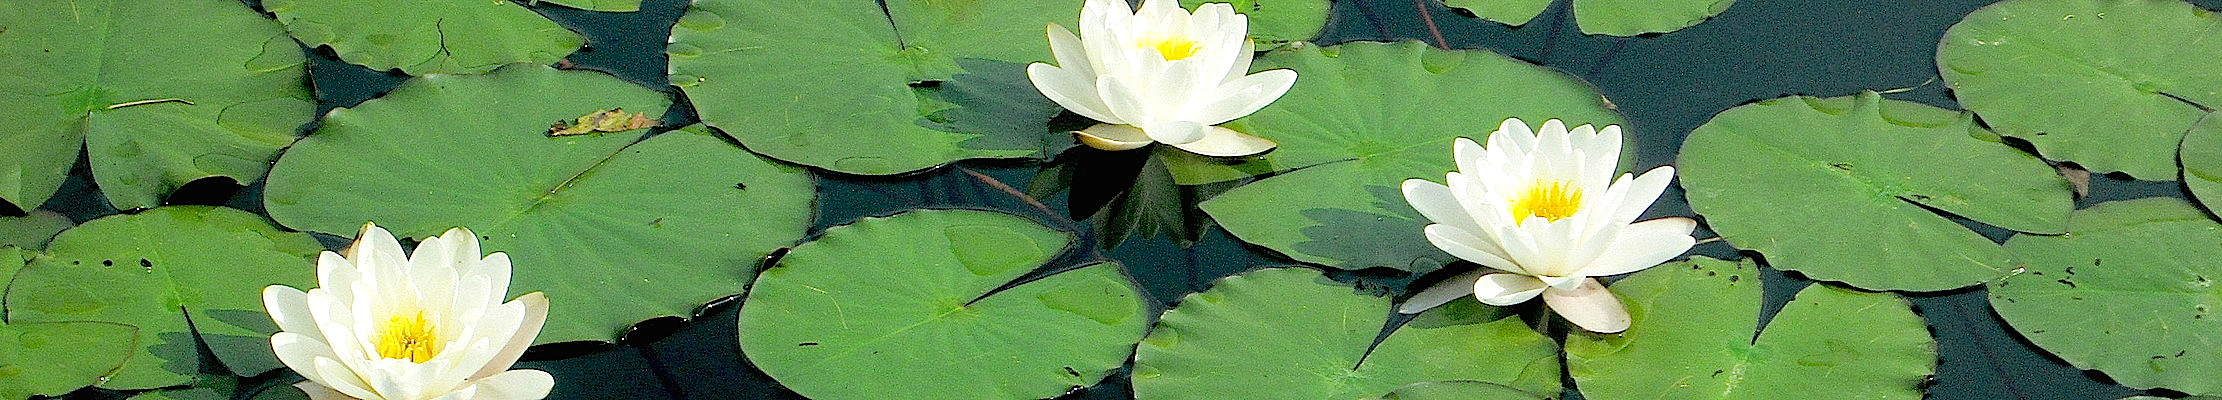
\includegraphics[width=1\linewidth]{img/Nymphaea_alba_pads} \caption{Photo of white water lillies on the water.}\label{fig:unnamed-chunk-46}
\end{figure}

As an instructive example, this lab will use the data from \citet{Law2014} on the petiole diameter (mm) from \emph{N. alba} collected from 7 different sites on the west coast of Scotland (the petiole is the structure that attaches the plant stem to the blade of the leaf).
The \emph{N. alba} dataset is available to download \href{https://raw.githubusercontent.com/bradduthie/SCIU4T4/main/data/Nymphaea_alba.csv}{here} (right click and ``Save Link As\ldots{}'').
Note that the data are not in a tidy format, so it is important to first reorganise the data so that they can be analysed in Jamovi (13.1).
Once the data are properly organised, we will use Jamovi to plot them (13.2), calculate summary statistics (13.3), apply appropriate decimals, significant figures, and rounding (13.4), and compare petiole diameters across sites (13.5).

\hypertarget{reorganise-the-dataset-into-a-tidy-format}{%
\section{Reorganise the dataset into a tidy format}\label{reorganise-the-dataset-into-a-tidy-format}}

The \emph{N. alba} dataset is not in a tidy format.
All of the numbers from this dataset are measurements of petiole diameter in mm from \emph{N. alba}, but each row contains 7 samples because each column shows a different site.
The full dataset is shown below.

\begin{verbatim}
##    Lily_Loch Choille.Bharr Creig.Moire Fidhle Buic Linne Beag
## 1       7.42          2.39        2.39   2.97 2.84  3.73 6.12
## 2       3.58          4.22        4.65   6.68 4.19  5.21 3.23
## 3       7.47          2.41        5.16   3.78 6.50  3.78 7.04
## 4       6.07          5.54        2.87   7.11 3.20  3.71 3.05
## 5       6.81          3.56        6.63   2.74 4.14  6.93 7.06
## 6       8.05          5.72        7.42   4.75 2.51  6.40 9.58
## 7       7.24          4.72        3.66   5.59 8.53  1.57 4.62
## 8       7.90          5.05        7.26   3.94 6.25  3.20 8.66
## 9       6.15          6.76        3.71   5.44 6.17  4.55 3.96
## 10      6.20          5.64        3.20   4.98 3.53  2.62 5.26
## 11      7.26          4.06        5.99   4.24 5.03  3.48 3.53
## 12      7.06          9.25        6.38   5.51 6.10  2.67 8.33
## 13      6.45          5.99        5.49   6.48 4.98  9.40 5.41
## 14      3.66          4.57        4.93   5.69 5.21  6.86 7.32
## 15      4.37          6.96        7.29   2.79 5.03  6.20 5.46
## 16      4.55          6.78        6.10   5.72 7.19  4.93 4.34
## 17      3.81          7.29        5.97   4.39 6.32  5.18 6.35
## 18      2.77          5.16        9.93   7.19 7.04  6.12 6.12
## 19      1.91          8.64        8.28   7.29 6.35  7.26 5.11
## 20      2.62          7.01        7.24   8.18 6.30  9.14 8.18
\end{verbatim}

Remember that to make these data tidy and usable in Jamovi, we need each row to be a unique observation.
What we really want then is a dataset with two columns of data.
The first column should indicate the site, and the second column should indicate the petiole diameter.
This can be done in two ways.
First, we could use a spreadsheet programme like LibreOffice or MS Excel to create a new dataset with two columns, one column with the site information and the other column with the petiole diameters.
Second, we could use the `Data' tab in Jamovi to create two new columns of data (one for site and the other for petiole diameter).
Either way, we need to copy and paste site names into the first column and petiole diameters in the second column.
This is a bit tedious, and we will not ask you to do it for every dataset, but it is an important step in the process of data analysis.
See Figure 13.2 for how this would look in Jamovi.

\begin{figure}
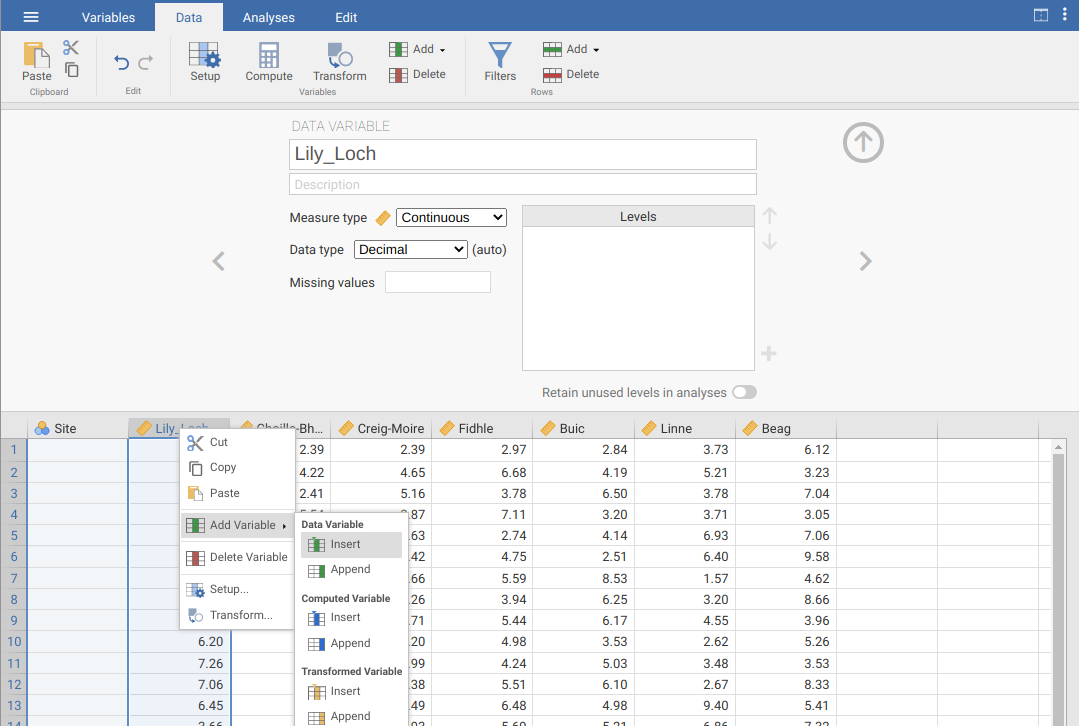
\includegraphics[width=1\linewidth]{img/lilypad_tidy} \caption{Tidying the raw data of petiole diameters from lily pad measurements across 7 sites in Scotland. A new column of data is created by right clicking on an existing column and choosing 'Add Variable'.}\label{fig:unnamed-chunk-48}
\end{figure}

Note that to insert a new column in Jamovi, we need to right click on an existing column and select `Add Variable' \(\to\) `Insert'.
A new column will then pop up in Jamovi, and we can give this an informative name.
Make sure to specify that the `Site' column should be a nominal measure type, and the `petiole\_diameter\_mm' column should be a continuous measure type.
The first 6 rows of the dataset should look like the below.

\begin{verbatim}
##        Site petiole_diameter_mm
## 1 Lily_Loch                7.42
## 2 Lily_Loch                3.58
## 3 Lily_Loch                7.47
## 4 Lily_Loch                6.07
## 5 Lily_Loch                6.81
## 6 Lily_Loch                8.05
\end{verbatim}

With the reorganised dataset, we are now ready to do some analysis in Jamovi.
We will start with some plotting.

\hypertarget{histograms-and-box-whisker-plots}{%
\section{Histograms and box-whisker plots}\label{histograms-and-box-whisker-plots}}

We will start by making a histogram of the full dataset of petiole diameter.
To do this, we need to go to the `Analyses' tab of the Jamovi toolbar, then select the `Exploration' button.

\begin{figure}
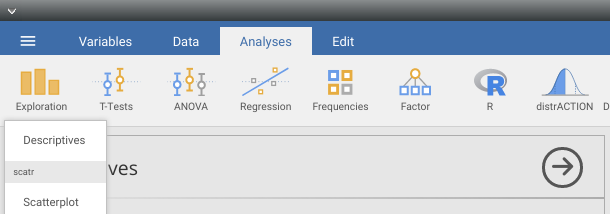
\includegraphics[width=1\linewidth]{img/lilypad_descriptives} \caption{Jamovi toolbar after having selected on the Analyses tab followed by the Exploration button.}\label{fig:unnamed-chunk-50}
\end{figure}

Next, select the `Descriptives' option (Figure 13.3).
This will open a new window where it is possible to create plots and calculate summary statistics.
The white box on the left of the Descriptive interface lists all of the variables in the dataset.
Below this box, there are options for selecting different summary statistics (`Statistics') and building different graphs (`Plots').
To get started, select the petiole diameter variable in the box to the left, then move it to the `Variables' box (top right) using the \(\to\) arrow.
Next, open the Plots option at the bottom of the interface.
Choose the `Histogram' option by clicking the checkbox.
A histogram will open up in the window on the right (you might need to scroll down).

\begin{figure}
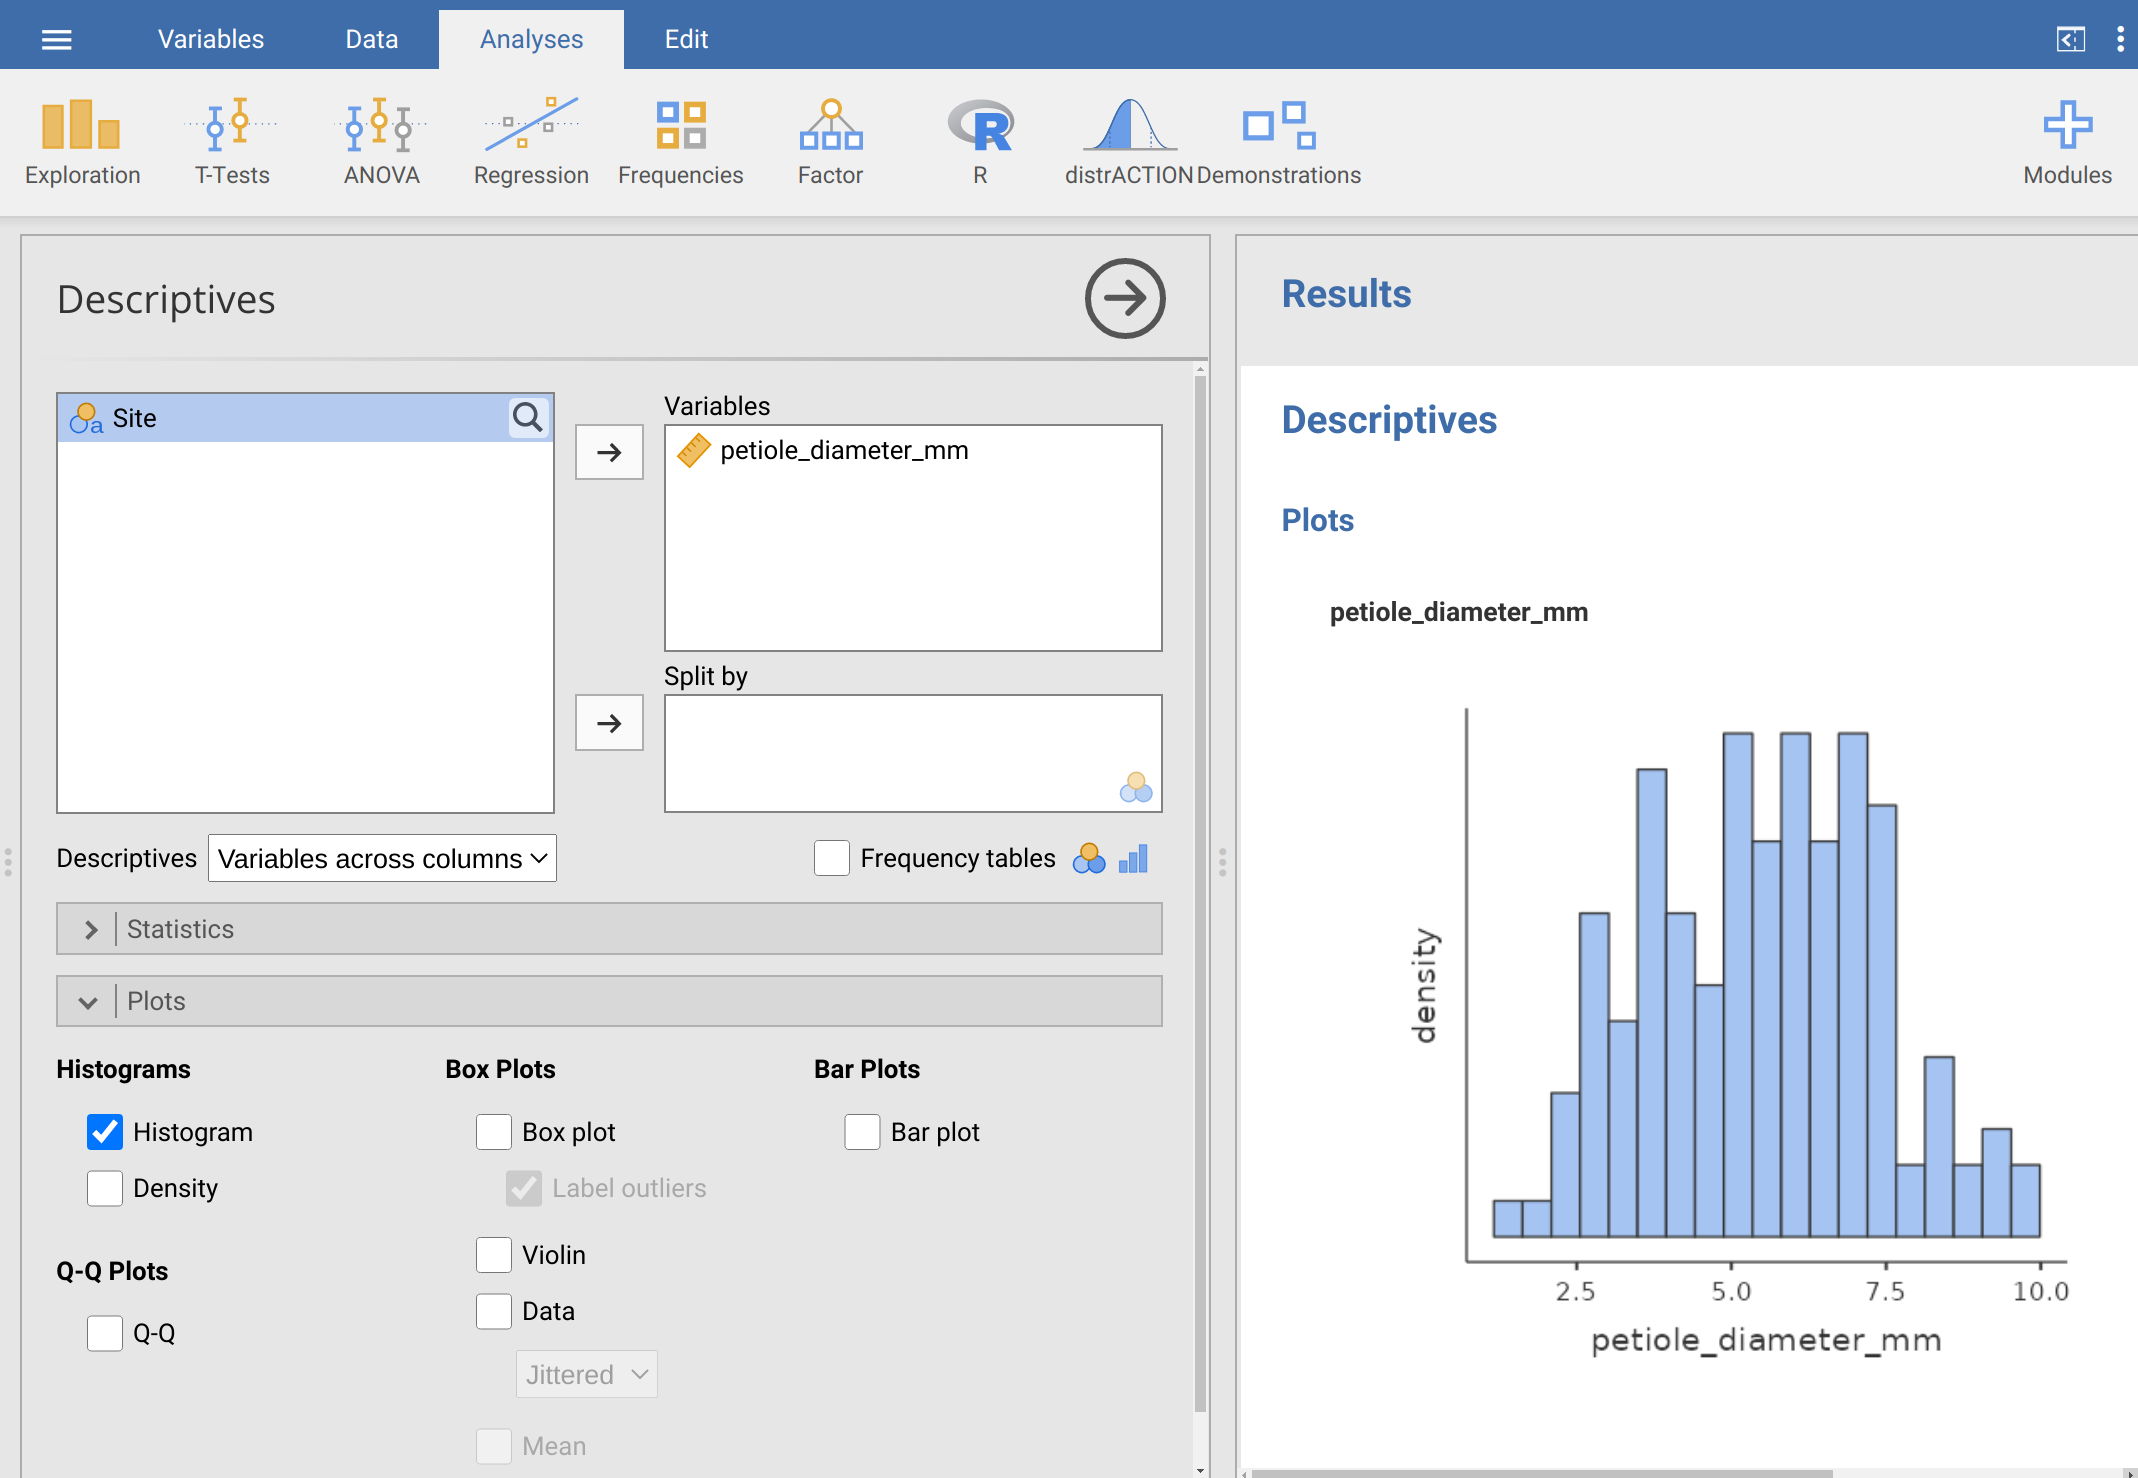
\includegraphics[width=1\linewidth]{img/lilypad_histogram} \caption{Jamovi Descriptives toolbar with petiole diameter selected and a histogram produced in the plotting window.}\label{fig:unnamed-chunk-51}
\end{figure}

Take a look at the histogram to the right (Figure 13.4).
Just looking at the histogram, write down what you think the following summary statistics will be.

Mean: \_\_\_\_\_\_\_\_\_\_\_\_\_\_\_\_\_\_\_\_\_\_\_\_\_\_\_\_

Median: \_\_\_\_\_\_\_\_\_\_\_\_\_\_\_\_\_\_\_\_\_\_\_\_\_\_\_\_

Standard deviation: \_\_\_\_\_\_\_\_\_\_\_\_\_\_\_\_\_\_\_\_\_\_\_\_\_\_\_\_

Based on the histogram, do you think that the mean and median are the same? Why or why not?

\begin{verbatim}






\end{verbatim}

The histogram needs better labelled axes and an informative caption.
To label the axes better, go back to the data tab and double click on the column heading `petiole\_diameter\_mm'.
Change the name of the data variable to `Petiole diameter (mm)'.
The newly named variable will then appear when a new histogram of the petiole diameter data is made.
To write a caption in Jamovi, click on the `Edit' tab at the very top of the toolbar.
You will see some blue boxes above and below the histogram, and you can write your caption by clicking on the box immediately below the histogram.
Write a caption for the histogram below.

\begin{verbatim}






\end{verbatim}

If you want to save the histogram, then you can right click on it.
A pop-up box will give you several options; select `Image \(\to\) Export' to save the histogram.
You can save it as a PDF, PNG, SVG, or EPS (if in doubt, PNG is probably the easiest to use).
You do not need to do this for this lab, but knowing how to do it will be useful for other modules, including your fourth year dissertation.

In the first example, we looked at petiole diameters across the entire dataset, but suppose that we want to see how the data are distributed for each site individually.
To do this, we just need to go back to the Descriptives box (Figure 13.4) and put the `Site' variable into the box on the lower right called `Split by'.
Do this by selecting `Site' then using the lower \(\to\) arrow to bring it to the `Split by' box.
Instead of one histogram of petiole diameters, you will now see 7 different histograms, one for each site, all stacked on top of each other.
This might be useful, but all of these histograms together are a bit busy.
Instead, we can use a box-whisker plot to compare the distributions of petiole diameters across different sites.

To create a box plot, simply check `Box plot' from the Plots options (you might want to uncheck `Histogram', but it is not necessary).
You should now see all of the different sites on the x-axis of the newly created boxplot and a summary of the petiole diameters on the y-axis.
Based on the boxplot, which site appears to have the highest and lowest median petiole diameter?

Highest: \_\_\_\_\_\_\_\_\_\_\_\_\_\_\_\_\_\_\_\_\_\_\_\_\_\_\_\_

Lowest: \_\_\_\_\_\_\_\_\_\_\_\_\_\_\_\_\_\_\_\_\_\_\_\_\_\_\_\_

There is one more trick with box-whisker plots in Jamovi that is useful.
The current plots show a summary of each site, but it might also be useful to plot the actual data points to give some more information about the distribution of petiole diameters.
You can do this by checking the option `Data', which places the petiole diameter of each sample over the box and whiskers for each site.
The y-axis shows the petiole diameter of each data point.
By default, the points are jittered on the x-axis, which just means that they are placed randomly on the x-axis within a site.
This is just to ensure that points will not be placed directly on top of each other if they are the same value.
If you prefer, you can use the pull-down menu right below the Data checkbox to select `Stacked' instead of `Jittered'
The stacked option will place points side by side.
Think about where the points are in relation to the box and whiskers of the plot; this should help you develop an intuitive understanding of how to read box-whisker plots.

\hypertarget{calculate-summary-statistics}{%
\section{Calculate summary statistics}\label{calculate-summary-statistics}}

We can calculate the summary statistics using the `Descriptives' option in Jamovi, just as we did with the histogram and box-whisker plots.
Before doing anything else, again place the petiole diameter variable in the box of variables, but do not split the dataset by site just yet because we first want summary statistics across the entire dataset.
Below the box of variables, but above the Plots options, there are options for selecting different summary statistics.
Open up this new box and have a look at the different summary statistics that can be calculated.
To calculate all of the variables explained in \protect\hyperlink{Chapter_11}{Chapter 11} and \protect\hyperlink{Chapter_11}{Chapter 12}, check the following 11 boxes:

\begin{itemize}
\tightlist
\item
  N: \_\_\_\_\_\_\_\_\_\_\_\_\_\_\_\_\_\_\_\_\_\_\_
\item
  Std. deviation: \_\_\_\_\_\_\_\_\_\_\_\_\_\_\_\_\_\_\_\_\_\_\_
\item
  Variance: \_\_\_\_\_\_\_\_\_\_\_\_\_\_\_\_\_\_\_\_\_\_\_
\item
  Minimum: \_\_\_\_\_\_\_\_\_\_\_\_\_\_\_\_\_\_\_\_\_\_\_
\item
  Maximum: \_\_\_\_\_\_\_\_\_\_\_\_\_\_\_\_\_\_\_\_\_\_\_
\item
  Range: \_\_\_\_\_\_\_\_\_\_\_\_\_\_\_\_\_\_\_\_\_\_\_
\item
  IQR: \_\_\_\_\_\_\_\_\_\_\_\_\_\_\_\_\_\_\_\_\_\_\_
\item
  Mean: \_\_\_\_\_\_\_\_\_\_\_\_\_\_\_\_\_\_\_\_\_\_\_
\item
  Median: \_\_\_\_\_\_\_\_\_\_\_\_\_\_\_\_\_\_\_\_\_\_\_
\item
  Mode: \_\_\_\_\_\_\_\_\_\_\_\_\_\_\_\_\_\_\_\_\_\_\_
\item
  Std. error of mean: \_\_\_\_\_\_\_\_\_\_\_\_\_\_\_\_\_\_\_\_\_\_\_
\end{itemize}

When you do this, the Statistics option in Jamovi should like like it does in Figure 13.5.

\begin{figure}
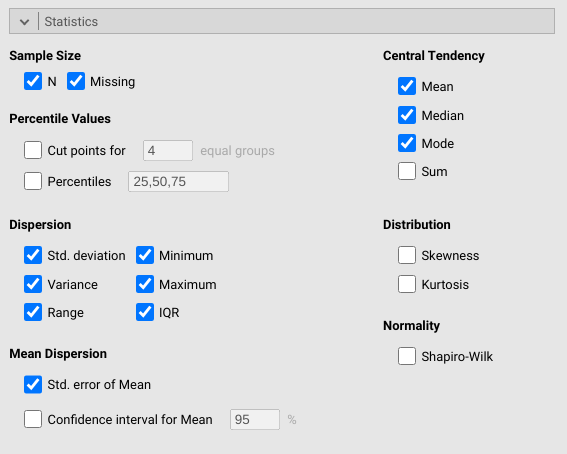
\includegraphics[width=1\linewidth]{img/lilypad_summary_statistics} \caption{Jamovi Descriptives toolbar showing the summary statistics available to report.}\label{fig:unnamed-chunk-52}
\end{figure}

Once you check these boxes, you will see a `Descriptives' table open on the right hand side of Jamovi.
This table will report all of the summary statistics that you have checked.
Write down the values for the summary statistics next to the corresponding bullet points above.

Next split these summary statistics up by site.
Notice the very large table that is now produced on the right hand side of Jamovi.
Which of the 7 sites in the data set has the highest mean petiole diameter, and what is its mean?

Site: \_\_\_\_\_\_\_\_\_\_\_\_\_\_\_\_\_\_\_\_\_\_\_\_\_\_\_\_\_\_

Mean: \_\_\_\_\_\_\_\_\_\_\_\_\_\_\_\_\_\_\_\_\_\_\_\_\_\_\_\_\_\_

Which of the 7 sites has the lowest variance in petiole diameter, and what is its variance?

Site: \_\_\_\_\_\_\_\_\_\_\_\_\_\_\_\_\_\_\_\_\_\_\_\_\_\_\_\_\_\_

Variance: \_\_\_\_\_\_\_\_\_\_\_\_\_\_\_\_\_\_\_\_\_\_\_\_\_\_\_\_\_\_

Make sure that you are able to find and interpret these summary statistics in Jamovi.
Explore different options to get more comfortable using Jamovi for building plots and reporting summary statistics.
Can you find the first and third quartiles for each site?
Report the third quartiles for each site below.

Beag: \_\_\_\_\_\_\_\_\_\_\_\_\_\_\_\_\_\_\_\_\_\_\_\_\_\_\_\_\_\_

Buic: \_\_\_\_\_\_\_\_\_\_\_\_\_\_\_\_\_\_\_\_\_\_\_\_\_\_\_\_\_\_

Choille-Bharr: \_\_\_\_\_\_\_\_\_\_\_\_\_\_\_\_\_\_\_\_\_\_\_\_\_\_\_\_\_\_

Creig-Moire: \_\_\_\_\_\_\_\_\_\_\_\_\_\_\_\_\_\_\_\_\_\_\_\_\_\_\_\_\_\_

Fidhle: \_\_\_\_\_\_\_\_\_\_\_\_\_\_\_\_\_\_\_\_\_\_\_\_\_\_\_\_\_\_

Lily\_Loch: \_\_\_\_\_\_\_\_\_\_\_\_\_\_\_\_\_\_\_\_\_\_\_\_\_\_\_\_\_\_

Linne: \_\_\_\_\_\_\_\_\_\_\_\_\_\_\_\_\_\_\_\_\_\_\_\_\_\_\_\_\_\_

Next, we will look at reporting summary statistics to different significant figures.

\hypertarget{reporting-decimals-and-significant-figures}{%
\section{Reporting decimals and significant figures}\label{reporting-decimals-and-significant-figures}}

Using the same values that you reported above for the whole dataset (i.e., not broken down by site), report each summary statistics to two significant figures.
Remember to round accurately if you need to reduce the number of significant figures from the original values to the new values below.
In assessments, you will often be asked to report a particular answer to a specific number of decimal places or significant figures, so the intention here is to help you practice.

\begin{itemize}
\tightlist
\item
  N: \_\_\_\_\_\_\_\_\_\_\_\_\_\_\_\_\_\_\_\_\_\_\_
\item
  Std. deviation: \_\_\_\_\_\_\_\_\_\_\_\_\_\_\_\_\_\_\_\_\_\_\_
\item
  Variance: \_\_\_\_\_\_\_\_\_\_\_\_\_\_\_\_\_\_\_\_\_\_\_
\item
  Minimum: \_\_\_\_\_\_\_\_\_\_\_\_\_\_\_\_\_\_\_\_\_\_\_
\item
  Maximum: \_\_\_\_\_\_\_\_\_\_\_\_\_\_\_\_\_\_\_\_\_\_\_
\item
  Range: \_\_\_\_\_\_\_\_\_\_\_\_\_\_\_\_\_\_\_\_\_\_\_
\item
  IQR: \_\_\_\_\_\_\_\_\_\_\_\_\_\_\_\_\_\_\_\_\_\_\_
\item
  Mean: \_\_\_\_\_\_\_\_\_\_\_\_\_\_\_\_\_\_\_\_\_\_\_
\item
  Median: \_\_\_\_\_\_\_\_\_\_\_\_\_\_\_\_\_\_\_\_\_\_\_
\item
  Mode: \_\_\_\_\_\_\_\_\_\_\_\_\_\_\_\_\_\_\_\_\_\_\_
\item
  Std. error of mean: \_\_\_\_\_\_\_\_\_\_\_\_\_\_\_\_\_\_\_\_\_\_\_
\end{itemize}

Remember from 13.2 that you were asked to write down what you thought the mean, median, and standard deviation were just by inspecting the histogram.
Compare your answers in that section with the rounded statistics listed above.
Were you able to get a similar value from the histogram as calculated in Jamovi from the data?
What can you learn from the histogram that you cannot from the summary statistics, and what can you learn from the summary statistics that you cannot from the histogram?
Write your reflections in the space below.

\begin{verbatim}






\end{verbatim}

Next, we will produce barplots to show the mean petiole diameter for each site.

\hypertarget{comparing-across-sites}{%
\section{Comparing across sites}\label{comparing-across-sites}}

To make a barplot that compares the mean petiole diameters across sites, we again use the Descriptives option in Jamovi.
Place petiole diameter as the variable, and spit this by site.
Next, go down to the plotting options and check `Bar plot'.
You will see a barplot produced in the window to the right with different sites on the x-axis.
Bar heights show the mean petiole diameter for each site.
Notice the intervals shown for each bar (i.e., the vertical lines in the centre of the bars that go up and down different lengths).
These error bars are centred on the mean petiole diameter (bar height) and show one standard error above and below the site mean.
Recall back from \protect\hyperlink{Chapter_12}{Chapter 12}; what information do these error bars convey about the estimated mean petiole diameter?

\begin{verbatim}






\end{verbatim}

What can you say about the mean petiole diameters across the different sites?
Do these sites appear to have very different mean petiole diameters?

\begin{verbatim}






\end{verbatim}

There were 20 total petiole diameters sampled from each site.
If we were to go back out to these 7 sites and sample another 20 petiole diameters, could we \textbf{really} expect to get the exact same site means?
Assuming the site means would be at least a bit different for our new sample, is it possible that the sites with the highest or lowest petiole diameters might also be different in our new sample?
If so, then what does this say about our ability to make conclusions about the differences in petiole diameter among sites?

\begin{verbatim}






\end{verbatim}

\hypertarget{part-probability-models-and-the-central-limit-theorem}{%
\part{Probability models and the Central Limit Theorem}\label{part-probability-models-and-the-central-limit-theorem}}

\hypertarget{Week4}{%
\chapter*{Week 4 Overview}\label{Week4}}
\addcontentsline{toc}{chapter}{Week 4 Overview}

\begin{longtable}[]{@{}
  >{\raggedright\arraybackslash}p{(\columnwidth - 2\tabcolsep) * \real{0.3269}}
  >{\raggedright\arraybackslash}p{(\columnwidth - 2\tabcolsep) * \real{0.6731}}@{}}
\toprule
\endhead
\textbf{Dates} & 13 February 2023 - 17 February 2023 \\
\textbf{Reading} & \textbf{Required:} SCIU4T4 Workbook chapters 14-15 \\
& \textbf{Recommended:} \citet{Navarro2022} \href{https://davidfoxcroft.github.io/lsj-book/07-Introduction-to-probability.html}{Chapter 7} \\
& \textbf{Suggested:} \citet{Rowntree2018} Chapter 4 \\
& \textbf{Advanced:} None \\
\textbf{Lectures} & 4.1: What is probability? (16:07 min; \href{https://stirling.cloud.panopto.eu/Panopto/Pages/Viewer.aspx?id=9b29a245-1921-4eec-8b89-af9e00aa8091}{Video}) \\
& 4.2: Adding and multiplying probabilities (16:18 min; \href{https://stirling.cloud.panopto.eu/Panopto/Pages/Viewer.aspx?id=ef35130e-6e18-4ae2-99d8-af9e00aca010}{Video}) \\
& 4.3: Probability distributions (15:30 min; \href{https://stirling.cloud.panopto.eu/Panopto/Pages/Viewer.aspx?id=f1860eb5-3ead-47ba-ad5f-af9e00ae26c2}{Video}) \\
& 4.4: The normal distribution (15:15 min; \href{https://stirling.cloud.panopto.eu/Panopto/Pages/Viewer.aspx?id=b4da1e5f-464f-4399-b427-af9e00b041e7}{Video}) \\
& 4.5: z-scores (5:12 min; \href{https://stirling.cloud.panopto.eu/Panopto/Pages/Viewer.aspx?id=4c46b6cf-bf60-4f30-b985-af9e00b32eb8}{Video}) \\
& 4.6: Examples using z-scores (13:22 min; \href{https://stirling.cloud.panopto.eu/Panopto/Pages/Viewer.aspx?id=a9d11e2f-5adc-434d-aeed-af9e00b403ab}{Video}) \\
& 4.7: More examples using z-scores (9:52 min; \href{https://stirling.cloud.panopto.eu/Panopto/Pages/Viewer.aspx?id=b3ad4395-6f50-4830-95b7-af9e00b56b3b}{Video}) \\
& 4.8: The binomial distribution (16:34 min; \href{https://stirling.cloud.panopto.eu/Panopto/Pages/Viewer.aspx?id=95be1330-0393-48b1-bfbc-af9e00b65f2e}{Video}) \\
& 4.9: The Poisson distribution (12:57 min; \href{https://stirling.cloud.panopto.eu/Panopto/Pages/Viewer.aspx?id=cdf67cc1-d8a9-48e5-a1dc-af9e00b8ca2e}{Video}) \\
& 4.10: The central limit theorem (5:21 min; \href{https://stirling.cloud.panopto.eu/Panopto/Pages/Viewer.aspx?id=f4026ecf-fdc4-40bd-9fc7-af9e00baffac}{Video}) \\
& 4.11: z-score tables (14:32 min; \href{https://stirling.cloud.panopto.eu/Panopto/Pages/Viewer.aspx?id=d286011d-e723-4fed-9a47-af9e00bbeb32}{Video}) \\
\textbf{Practical} & Probability and simulation (\protect\hyperlink{Chapter_16}{Chapter 16}) \\
& Room: Cottrell 2A17 \\
& Group A: 15 FEB 2023 (WED) 13:05-15:55 \\
& Group B: 16 FEB 2023 (THU) 09:05-11:55 \\
\textbf{Help hours} & Ian Jones \\
& Room: Cottrell 3V1B \\
& 17 FEB 2023 (FRI) 15:05-17:55 \\
\textbf{Assessments} & \href{https://canvas.stir.ac.uk/courses/13075/quizzes/29675}{Week 4 Practice quiz} on Canvas \\
\bottomrule
\end{longtable}

Week 4 focuses on probability and the central limit theorem.

\protect\hyperlink{Chapter_14}{Chapter 14} introduces probability models and how to interpret them.
The chapter also provides some examples of probability distributions that are especially relevant to biological and environmental sciences.

\protect\hyperlink{Chapter_15}{Chapter 15} focuses on the central limit theorem (CLT), what it is, and why it is so important in statistics.

\protect\hyperlink{Chapter_16}{Chapter 16} guides you through the week 4 practical.
The aim of this practical is to apply the ideas from \protect\hyperlink{Chapter_14}{Chapter 14} and \protect\hyperlink{Chapter_15}{Chapter 15} in Jamovi to predict probabilities from a real dataset.

\hypertarget{Chapter_14}{%
\chapter{Introduction to probability models}\label{Chapter_14}}

Suppose that we flip a fair coin over a flat surface.
There are two possibilities for how the coin lands on the surface.
Either the coin lands on one side (heads) or the other side (tails), but we do not know the outcome in advance.
If these two events (heads or tails) are equally likely, then we could reason that there is a 50\% chance that a flipped coin will land heads up and a 50\% chance that it will land heads down.
What do we actually mean when we say this?
For example, when we say that there is a 50\% chance of the coin landing heads up, are we making a claim about our own uncertainty, how coins work, or how the world works?
We might mean that we simply do not know whether or not the coin will land heads up, so a 50-50 chance just reflects our own ignorance about what will actually happen when the coin is flipped.
Alternatively, we might reason that if a fair coin were to be flipped many times, all else being equal, then about half of flips should end heads up, so a 50\% chance is a reasonable prediction of what will happen in any given flip.
Or, perhaps we reason that events such as coin flips really are guided by chance on some deeper fundamental level, such that our 50\% chance reflects some real causal metaphysical process in the world.
These are questions concerning the philosophy of probability.
The philosophy of probability is an interesting sub-discipline in its own right, with implications that can and do affect how researchers do statistics \citep{Edwards1972, Mayo1996, Gelman2013, Suarez2020, Mayo2021, Navarro2022}.

In this chapter, we will not worry about the philosophy of probability\footnote{In the interest of transparency, this book presents a \emph{frequentist} interpretation of probability \citep{Mayo1996}. While this approach does reflect the philosophical inclinations of the author, the reason for working from this interpretation has more to do with the statistical tests that are most appropriate for an introductory statistics module, which are also the tests most widely used in the biological and environmental sciences.} and instead focus on the mathematical rules of probability as applied to statistics.
These rules are important for predicting real-world events in the biological and environmental sciences.
For example, we might need to make predictions concerning the risk of disease spreading in a population, or the risk of extreme events such as droughts occurring given increasing global temperatures.
Probability is also important for testing scientific hypotheses.
For example, if we sample two different groups and calculate that they have different means (e.g., two different fields have different mean soil nitrogen concentrations), we might want to know the probability that this difference between means could have arisen by chance.
Here we will introduce practical examples of probability, then introduce some common probability distributions.

\hypertarget{an-instructive-example}{%
\section{An instructive example}\label{an-instructive-example}}

Probability focuses on the outcomes of trials, such as the \textbf{outcome} (heads or tails) of the \textbf{trial} of a coin flip.
The probability of a specific outcome is the relative number of times it is expected to happen given a large number of trials,

\[P(outcome) = \frac{Number\:of\:times\:outcome\:occurs}{Total\:number\:of\:trials}.\]

For the outcome of a flipped coin landing on heads,

\[P(heads) = \frac{Flips\:landing\:on\:heads}{Total\:number\:of\:flips}.\]

As the total number of flips becomes very large, the number of flips that land on heads should get closer and closer to half the total, \(1/2\) or \(0.5\) (more on this later).
The above equations use the notation \(P(E)\) to define the probability (\(P\)) of some event (\(E\)) happening.
Note that the number of times an outcome occurs cannot be less than 0, so \(P(E) \geq 0\) must always be true.
Similarly, the number of times an outcome occurs cannot be greater than the number of trials; the most frequently it can happen is in \emph{every} trial, in which case the top and bottom of the fraction has the same value.
Hence, \(P(E) \leq 1\) must also always be true.
Probabilities therefore range from 0 (an outcome \emph{never} happens) to 1 (an outcome \emph{always} happens).

It might be more familiar and intuitive at first to think in terms of percentages (i.e., from 0-100\% chance of an outcome, rather than from 0-1), but there are good mathematical reasons for thinking about probability on a 0-1 scale (it makes calculations easier).
For example, suppose we have two coins, and we want to calculate the probability that they will both land on heads if we flip them at the same time.
That is, we want to know the probability that coin 1 lands on heads \textbf{and} coin 2 lands on heads.
We can assume that the coins do not affect each other in any way, so each coin flip is \textbf{independent} of the other (i.e., the outcome of coin 1 does not affect the outcome of coin 2, and \emph{vice versa} -- this kind of assumption is often very important in statistics).
Each coin, by itself, is expected to land on heads with a probability of 0.5, \(P(heads) = 0.5\).
When we want to know the probability that two or more independent events will happen, we \emph{multiply} their probabilities.
In the case of both coins landing on heads, the probability is therefore,

\[P(Coin_{1} = heads\:\cap Coin_{2} = heads) = 0.5 \times 0.5 = 0.25.\]

Note that the symbol \(\cap\) is basically just a fancy way of writing `and' (technically, the intersection between sets; see set theory for details).
Verbally, all this is saying is that the probability of coin 1 landing on heads \emph{and} the probability of coin 2 landing on heads equals 0.5 times 0.5, which is 0.25.

But why are we \emph{multiplying} to get the joint probability of both coins landing on heads?
Why not add, for example?
We could just take it as a given that multiplication is the correct operation to use when calculating the probability that multiple events will occur.
Or we could do a simple experiment to confirm that 0.25 really is about right (e.g., by flipping 2 coins 100 times and recording how many times both coins land on heads).
But neither of these options would likely be particularly satisfying.
Let us first recognise that adding the probabilities cannot be the correct answer.
If the probability of each coin landing on heads is 0.5, then adding probabilities would imply that the probability of both landing on heads is 0.5 + 0.5 = 1.
This does not make any sense because we know that there are other possibilities, such as both coins landing on tails, or one coin landing on heads and the other landing on tails.
Adding probabilities cannot be the answer, but why multiply?

We can think about probabilities visually, as a kind of probability space.
When we have only one trial, then we can express the probability of an event along a line (Figure 14.1).

\begin{figure}
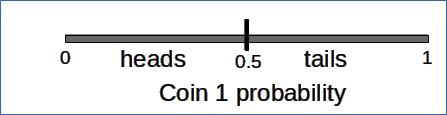
\includegraphics[width=1\linewidth]{img/coin1_probability} \caption{Total probability space for flipping a single coin and observing its outcome (heads or tails). Given a fair coin, the probability of heads equals a proportion 0.5 of the total probability space, while the probability of tails equals the remaining 0.5 proportion.}\label{fig:unnamed-chunk-53}
\end{figure}

The total probability space is 1, and `heads' occupies a density of 0.5 of the total space.
The remaining space, also 0.5, is allocated to `tails'.
When we add a second independent trial, we now need 2 dimensions of probability space (Figure 14.2).
The probability of heads or tails for coin 1 (the horizontal axis of Figure 14.2) remains unchanged, but we add another axis (vertical this time) to think about the equivalent probability space of coin 2.

\begin{figure}
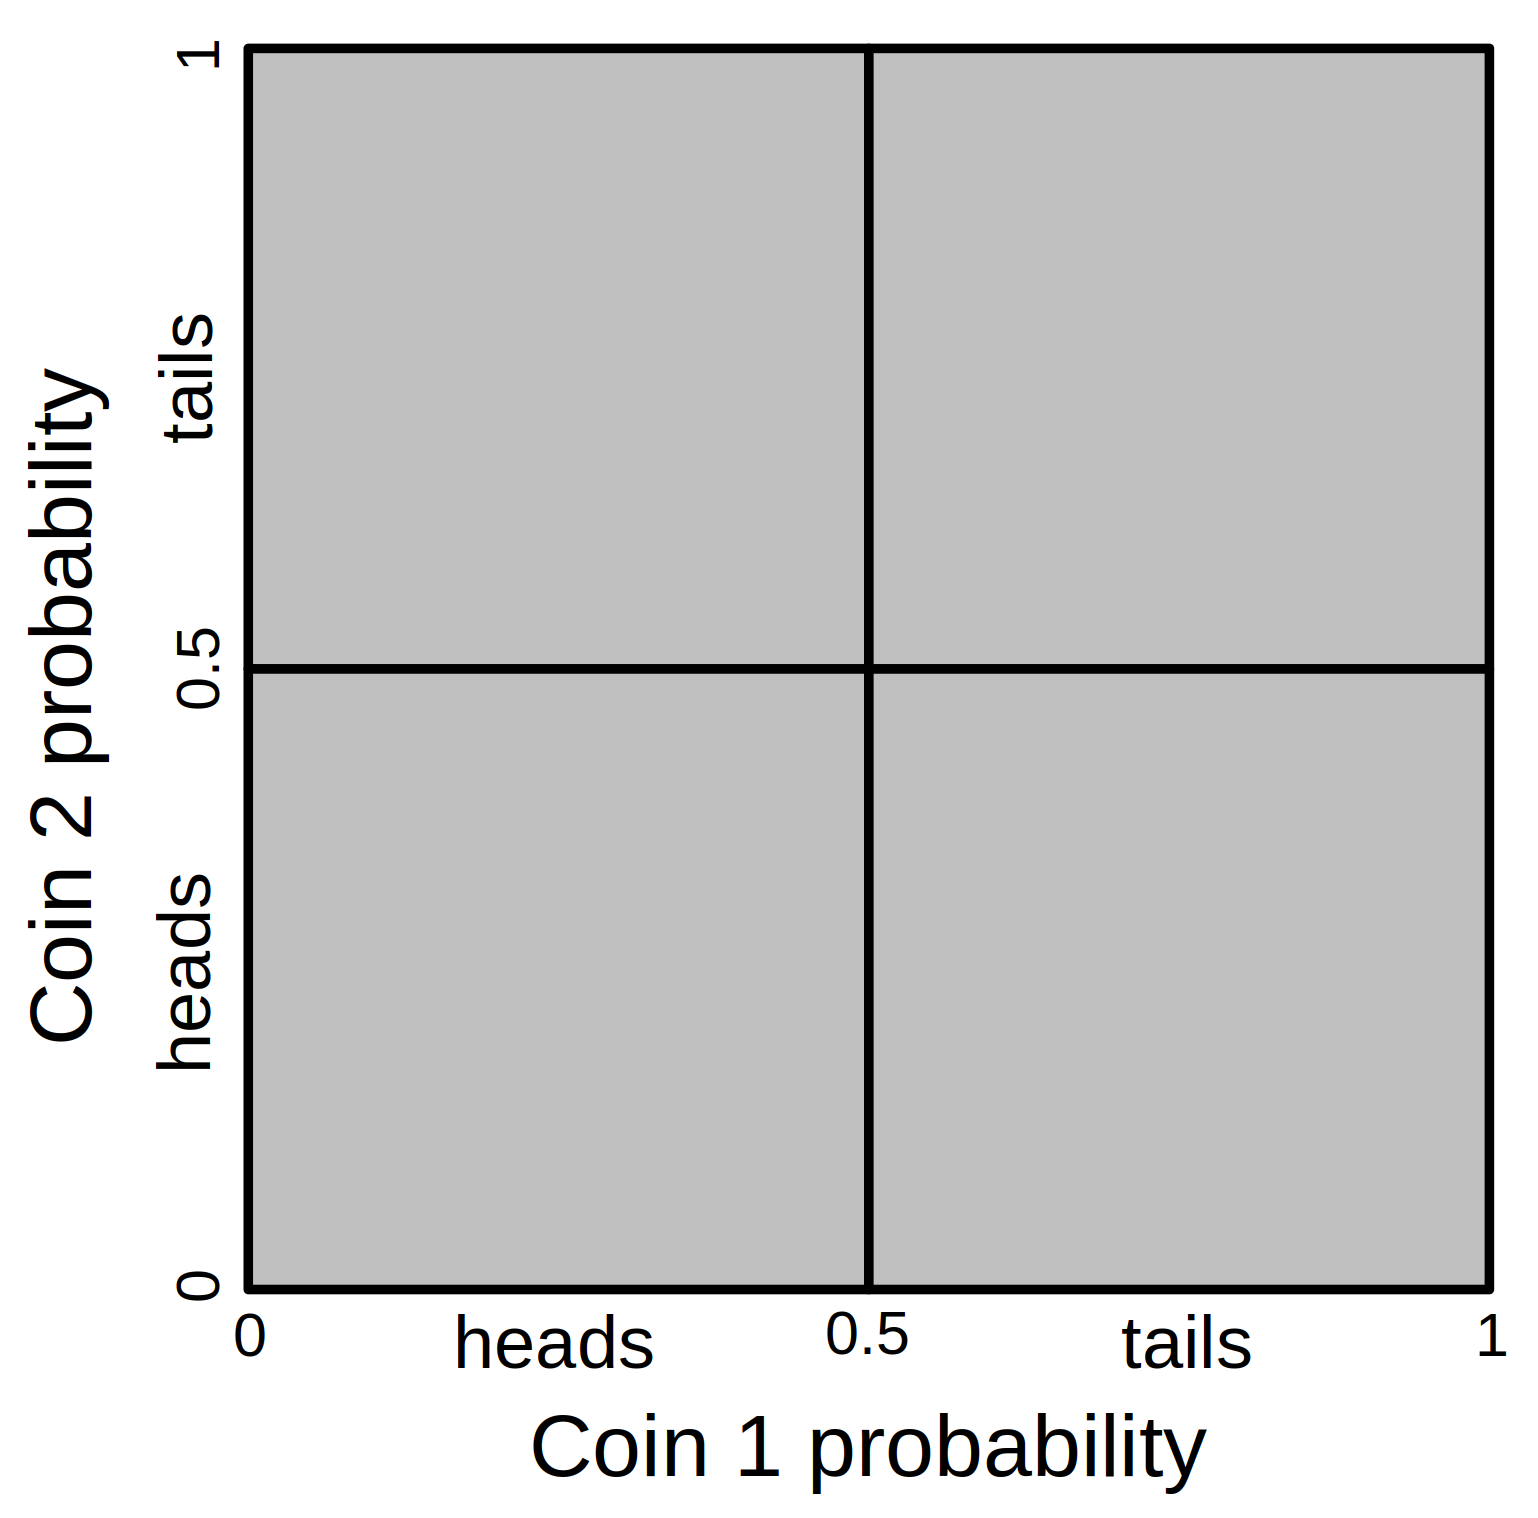
\includegraphics[width=1\linewidth]{img/coin2_probability} \caption{Total probability space for flipping two coins and observing their different possible outcomes (heads-heads, heads-tails, tails-heads, and tails-tails). Given two fair coins, the probability of flipping each equals 0.25, which corresponds to the lower left square of the probability space.}\label{fig:unnamed-chunk-54}
\end{figure}

Now we can see that that the area in which both coin 1 and coin 2 land on heads has a proportion of 0.25 of the total area.
This is a geometric representation of what we did when calculating \(P(Coin_{1} = heads\:\cap Coin_{2} = heads) = 0.5 \times 0.5 = 0.25.\)
The multiplication works because multiplying probabilities carves out more specific regions of probability space.
Note that the same pattern would apply if we flipped a third coin.
In this case, the probability of all 3 coins landing on heads would be \(0.5 \times 0.5 \times 0.5 = 0.125\), or \(0.5^{3} = 0.125\).

What about when we want to know the probability of one outcome \textbf{or} another outcome happening?
Here is where we add.
Note that the probability of a coin flip landing on heads or tails must be 1 (there are only 2 possibilities!).
What about the probability of both coins landing on the same outcome; that is, either both coins landing on heads or both landing on tails?
We know that the probability of both coins landing on heads is \(0.25\).
The probability of both coins landing on tails is also \(0.25\), so the probability that both coins land on either heads \textbf{or} tails is \(0.25 + 0.25 = 0.5\).
The visual representation in Figure 14.2 works for this example too.
Note that heads-heads and tails-tails outcomes are represented by the lower left and upper right areas of probability space, respectively.
This is 0.5 (i.e., 50\%) of the total probability space.

\hypertarget{biological-applications}{%
\section{Biological applications}\label{biological-applications}}

Coin flips are instructive, but the relevance for biological and environmental sciences might not be immediately clear.
In fact, probability is extremely relevant in nearly all areas of the natural sciences.
The following are just 2 hypothetical examples where the calculations in the previous section might be usefully applied:

\begin{enumerate}
\def\labelenumi{\arabic{enumi}.}
\item
  From a recent report online, suppose you learn that 1 in 40 people in your local area are testing positive for Covid-19. You find yourself in a small shop with 6 other people. What is the probability that at least 1 of these 6 other people would test positive for Covid-19? To calculate this, note that the probability that any given person has Covid-19 is \(1/40 = 0.025\), which means that the probability that a person does \textbf{not} must be \(1 - 0.025 = 0.975\) (they either do or do not, and the probabilities must sum to 1). The probability that \textbf{all} 6 people \emph{do not} have Covid-19 is therefore \((0.975)^6 = 0.859\). Consequently, the probability that at least 1 of the 6 people \textbf{does} have Covid-19 is \(1 - 0.859 = 0.141\), or \(14.1\%\).
\item
  Imagine you are studying a population of sexually reproducing, diploid (i.e., 2 sets of chromosomes), animals, and you find that a particular genetic locus has 3 alleles with frequencies \(P(A_{1}) = 0.40\), \(P(A_{2}) = 0.45\), and \(P(A_{3}) = 0.15\). What is the probability that a randomly sampled animal will be heterozygous with 1 copy of the \(A_{1}\) allele and 1 copy of the \(A_{3}\) allele? Note that there are 2 ways for \(A_{1}\) and \(A_{3}\) to arise in an individual, just like there were 2 ways to get a heads and tails coin in the section 14.1 example (see Figure 14.2). The individual could either get an \(A_{1}\) in the first position and \(A_{3}\) in the second position, or an \(A_{3}\) in the first position and \(A_{1}\) in the second position. We can therefore calculate the probability as, \(P(A_{1}) \times P(A_{3}) + P(A_{3}) \times P(A_{1})\), which is \((0.40 \times 0.15) + (0.15 \times 0.4) = 0.12\), or 12\% (in population genetics, we might use the notation \(p = P(A_{1})\) and \(r = P(A_{3})\), then note that \(2pr = 0.12\)).
\end{enumerate}

In both of these examples, we made some assumptions, which might or might not be problematic.
In the first example, we assumed that the 6 people in our shop were a random and independent sample from the local area (i.e., people with Covid-19 are not more or less likely to be in the shop, and the 6 people in the shop were not associated in a way that would affect their individual probabilities of having Covid-19).
In the second example, we assumed that individuals mate randomly, and that there is no mutation, migration, or selection on genotypes \citep{Hardy1908}.
It is important to recognise these assumptions when we are making them because violations of assumptions could affect the probabilities of events!

\hypertarget{sampling-with-and-without-replacement}{%
\section{Sampling with and without replacement}\label{sampling-with-and-without-replacement}}

It is often important to make a distinction between sampling with or without replacement.
Sampling with replacement just means that whatever has been sampled once gets put back into the population before sampling again.
Sampling without replacement means that whatever has been sampled does not get put back into the population before sampling again.
An example makes the distinction between sampling with and without replacement clearer.

\begin{figure}
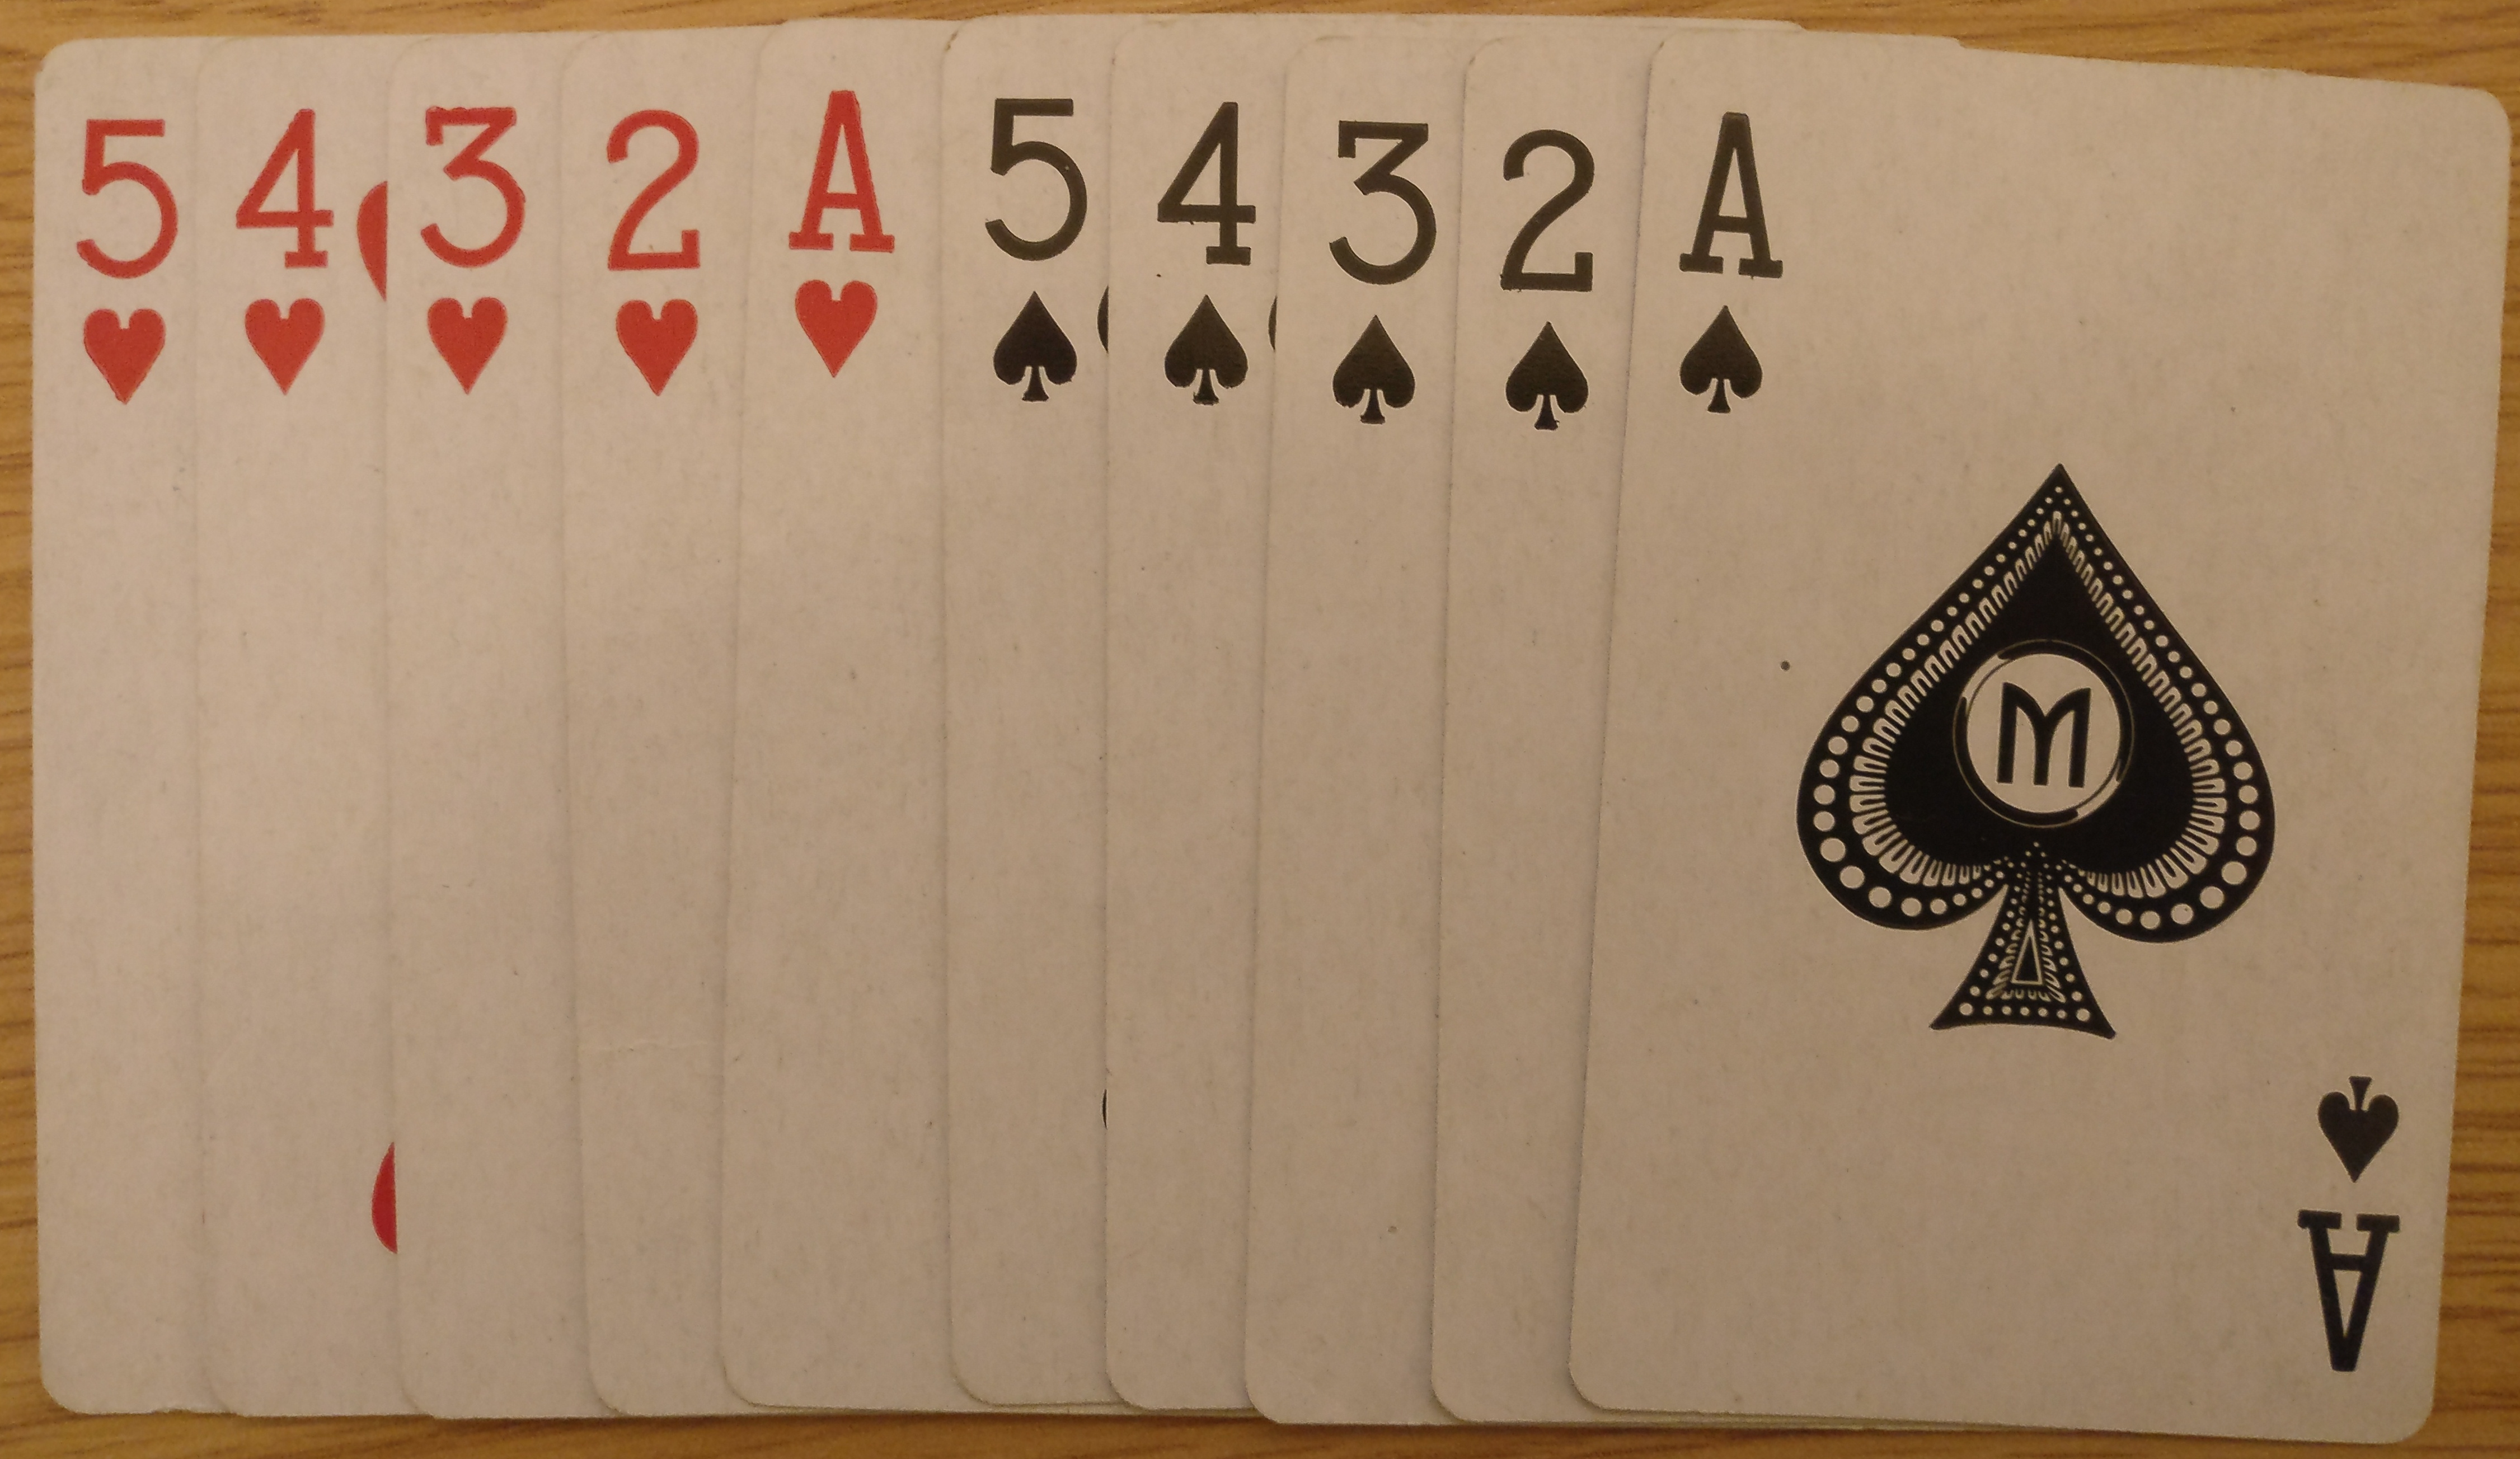
\includegraphics[width=1\linewidth]{img/cards} \caption{Playing cards can be useful for illustrating concepts in probability. Here we have 5 hearts (left) and 5 spades (right).}\label{fig:unnamed-chunk-55}
\end{figure}

Figure 14.3 shows 10 playing cards, 5 hearts and 5 spades.
If we shuffle these cards thoroughly and randomly select 1 card, what is the probability of selecting a heart?
This is simply,

\[P(heart) = \frac{5\:hearts}{10\:total\:cards} = 0.5.\]

What is the probability of randomly selecting 2 hearts?
This depends if we are sampling with or without replacement.
If we sample 1 card, then put it back into the deck before sampling the second card, then the probability of sampling a heart does not change (in both samples, we have 5 hearts and 10 cards).
Hence, the probability of sampling two hearts with replacement is \(P(heart) \times P(heart) = 0.5 \times 0.5 = 0.25\).
If we do not put the first card back into the deck before sampling again, then we have changed the total number of cards.
After sampling the first heart, we have one fewer hearts in the deck and one fewer cards, so the new probability for sampling a heart becomes,

\[P(heart) = \frac{4\:hearts}{9\:total\:cards} = 0.444.\]

Since the probability has changed after the first heart is sampled, we need to use this adjusted probability when sampling without replacement.
In this case, the probability of sampling two hearts is \(0.5 \times 0.444 = 0.222\).
This is a bit lower than the probability of sampling with replacement because we have decreased the number of hearts that can be sampled.
When sampling from a set, it is important to consider whether the sampling is done with or without replacement (in assessments, we will always make this clear).

\hypertarget{probability-distributions}{%
\section{Probability distributions}\label{probability-distributions}}

Up until this point, we have been considering the probabilities of specific outcomes.
That is, we have considered the probability that a coin flip will be heads, that an animal will have a particular combination of alleles, or that we will randomly select a particular suit of card from a deck.
Here we will move from specific outcomes and consider the \emph{distribution} of outcomes.
For example, instead of finding the probability that a flipped coin lands on heads, we might want to consider the distribution of the number of times that it does (in this case, 0 times or 1 time).

\begin{figure}
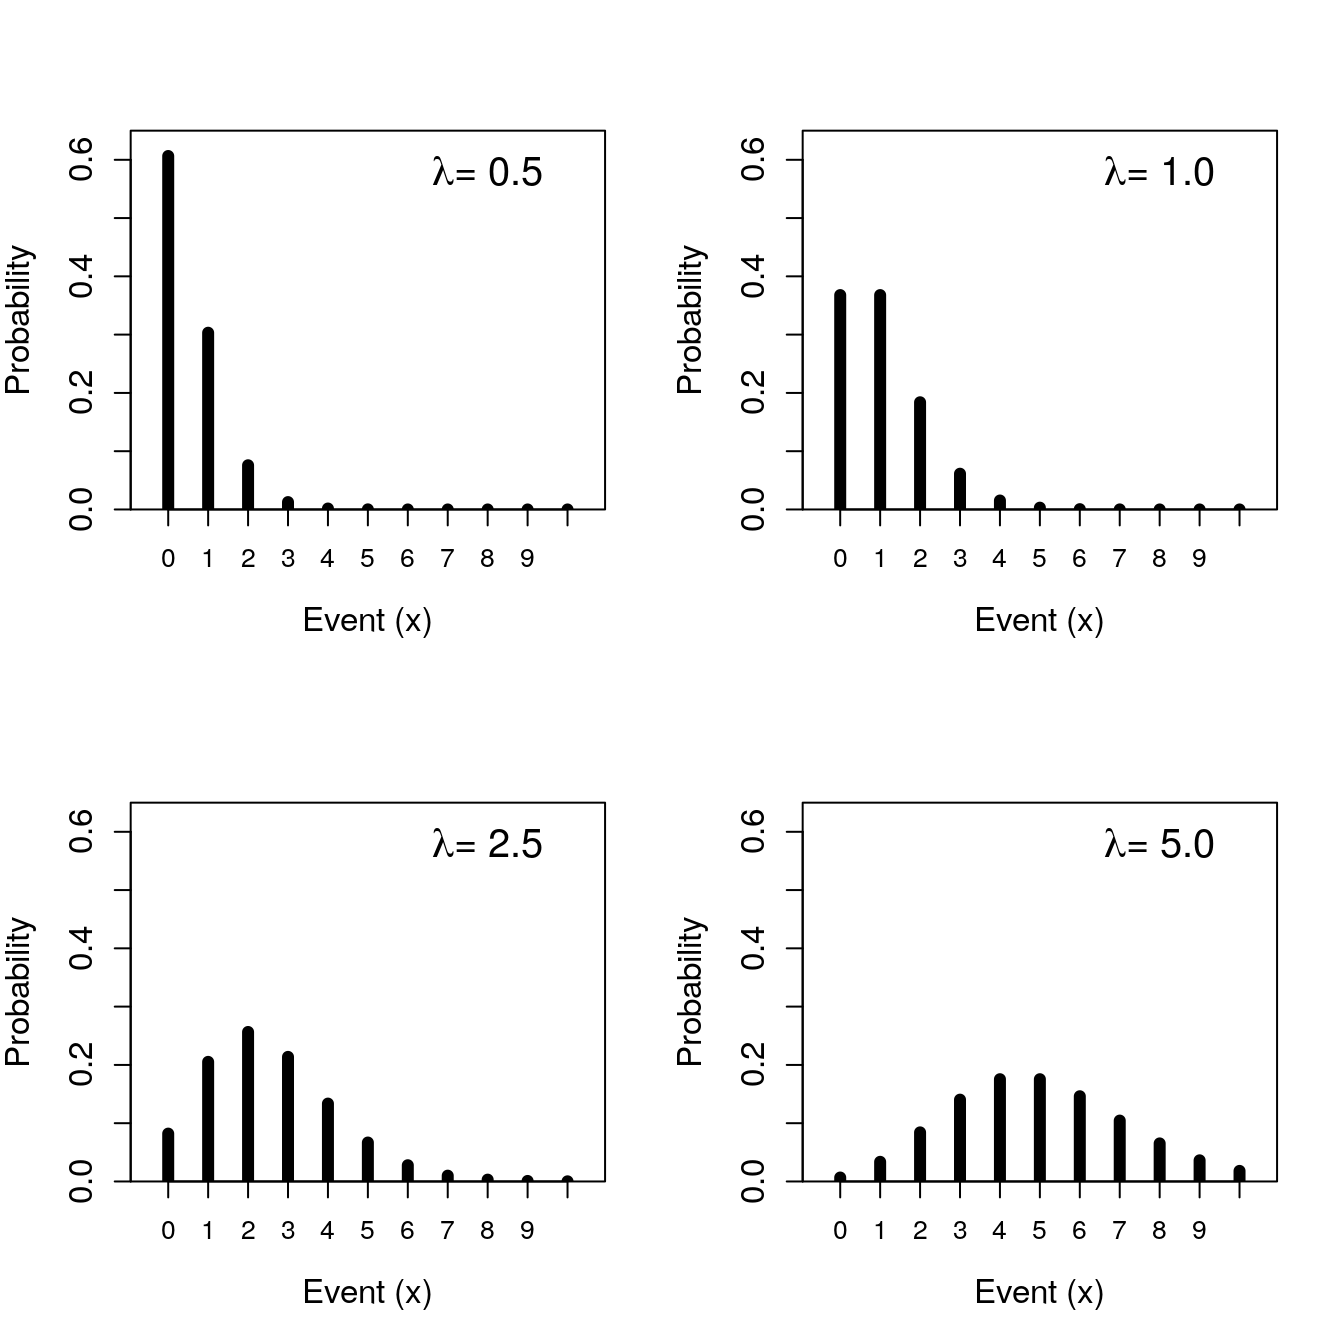
\includegraphics{bookdown-demo_files/figure-latex/unnamed-chunk-56-1} \caption{Probability distribution for the number of times that a flipped coin lands on heads in 1 trial.}\label{fig:unnamed-chunk-56}
\end{figure}

This is an extremely simple distribution.
There are only two discrete possibilities for the number of times the coin will land on heads, 0 or 1.
And the probability of both outcomes is 0.5, so the bars in Figure 14.4 are the same height.
Next, we will consider some more interesting distributions.

\hypertarget{binomial-distribution}{%
\subsection{Binomial distribution}\label{binomial-distribution}}

The simple distribution with a single trial of a coin flip was actually an example of a binomial distribution.
More generally, a binomial distribution describes the number of successes in some number of trials \citep{Miller2004}.
The word `success' should not be taken too literally here; it does not necessarily indicate a good outcome, or an accomplishment of some kind.
A success in the context of a binomial distribution just means that an outcome \emph{did} happen as opposed to it \emph{not} happening.
If we define a coin flip landing on heads as a success, we could consider the probability distribution of the number of successes over 10 trials (Figure 14.5)

\begin{figure}
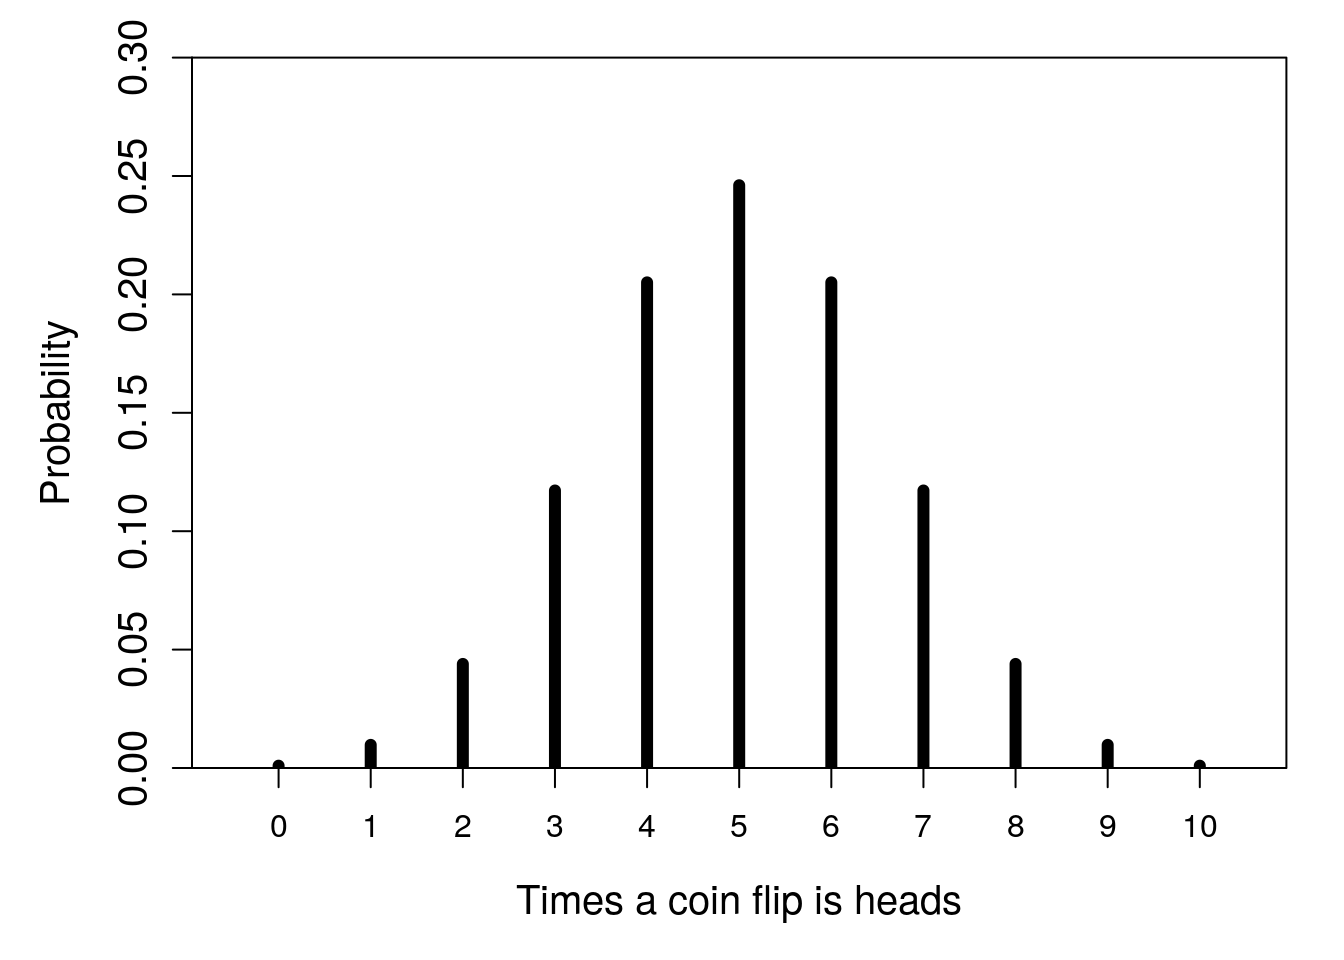
\includegraphics{bookdown-demo_files/figure-latex/unnamed-chunk-57-1} \caption{Probability distribution for the number of times that a flipped coin lands on heads in 10 trials.}\label{fig:unnamed-chunk-57}
\end{figure}

Figure 14.5 shows that the most probable outcome is that 5 of the 10 coins flipped will land on heads.
This makes some sense because the probability that any 1 flip lands on heads is 0.5, and 5 is 1/2 of 10.
But 5 out of 10 heads happens only with a probability of about 0.25.
There is also about a 0.2 probability that the outcome is 4 heads, and the same probability that the outcome is 6 heads.
Hence, the probability that we get an outcome of between 4-6 heads is about \(0.25 + 0.2 + 0.2 = 0.65\).
In contrast, the probability of getting all heads is very low (about 0.00098).

More generally, we can define the number of successes using the random variable \(X\).
We can then use the notation \(P(X = 5) = 0.25\) to indicate the probability of 5 successes, or \(P(4 \leq X \leq 6) = 0.65\) as the probability that the number of successes is greater than or equal to 4 and less than or equal to 6.

Imagine that you were told a coin was fair, then flipped it 10 times.
Imagine that 9 flips out of the 10 came up heads.
Given the probability distribution shown in Figure 14.5, the probability of getting 9 or more heads in 10 flips given a fair coin is very low (\(P(X \geq 9) \approx 0.011\)).
Would you still believe that the coin is fair after these 10 trials?
How many, or how few, heads would it take to convince you that the coin was not fair?
This question gets to the heart of a lot of hypothesis-testing in statistics, and we will discuss it more in Week 6.

Note that a binomial distribution does not need to involve a fair coin with equal probability of success and failure.
We can consider again the first example in Section 14.2, in which 1 in 40 people in an area are testing positive for Covid-19, then ask what the probability is that 0-6 people in a small shop would test positive (Figure 14.6).

\begin{figure}
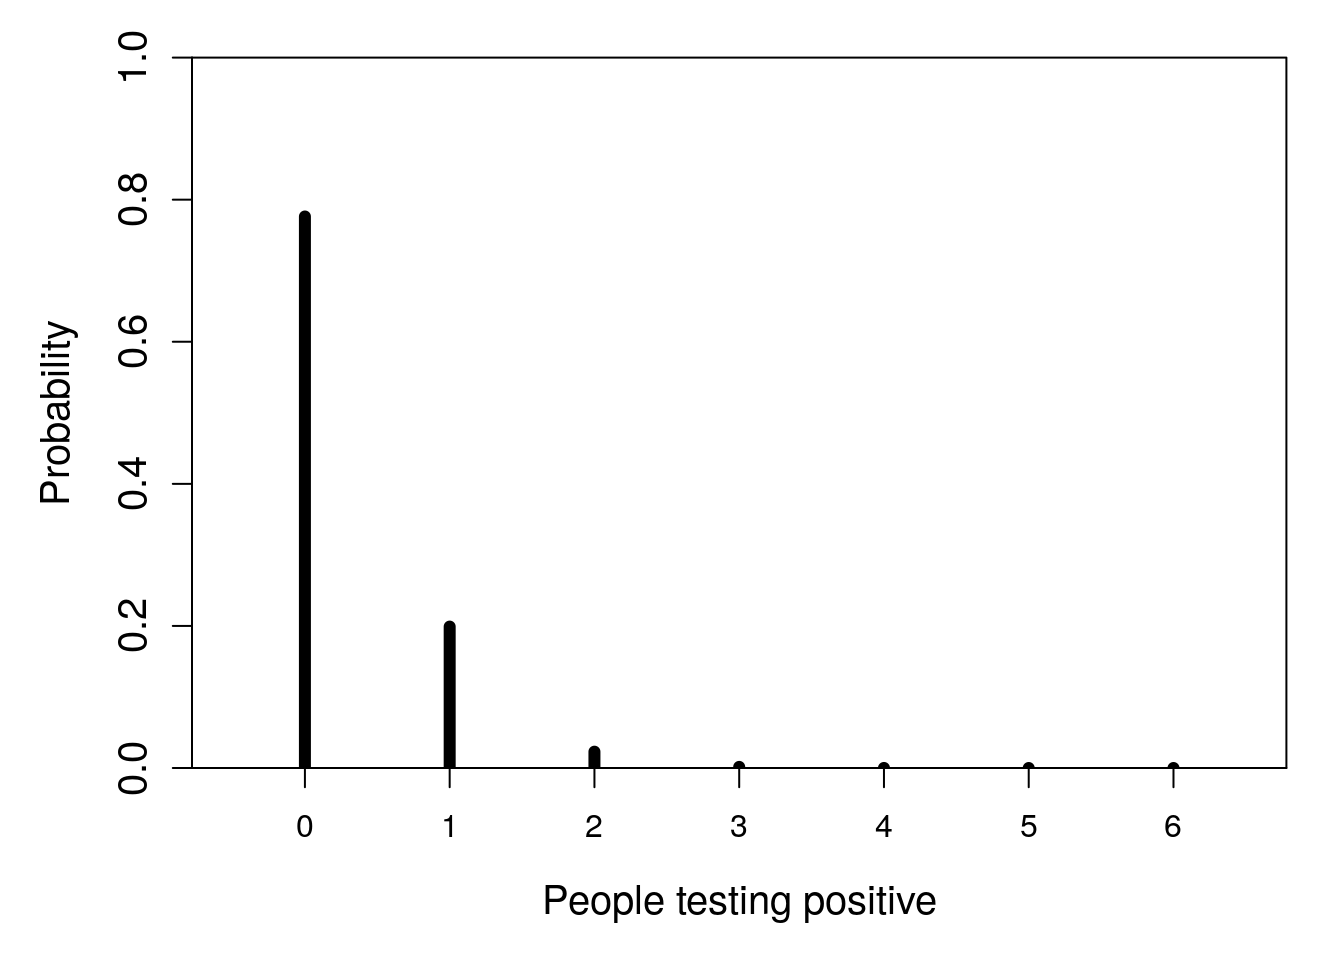
\includegraphics{bookdown-demo_files/figure-latex/unnamed-chunk-58-1} \caption{Probability distribution for the number of people who have Covid-19 in a shop of 6 when the probability of testing positive is 0.025.}\label{fig:unnamed-chunk-58}
\end{figure}

Note that the shape of this binomial distribution is different from the coin flipping trials in Figure 14.5.
The distribution is skewed, with a high probability of 0 successes and a diminishing probability of 1 or more successes.

The shape of a statistical probability distribution can be defined mathematically.
Depending on the details (more on this later), we call the equation defining the distribution either a probability mass function or a probability density function.
This book is about statistical techniques, not statistical theory, so we will relegate these equations to footnotes.\footnote{For those interested, more technically, we can say that a random variable \(X\) has binomial distribution if and only if its probability mass function is defined by \citep{Miller2004}, \[b \left(x; n, \theta \right) = {n \choose x} \theta^{x} \left(1 - \theta\right)^{n-x}.\] In this binomial probability mass function, \(x = 0, 1, 2, ..., n\) (i.e., \(x\) can take any integer value from 0 to n). Note that the \(n\) over the \(x\) in the first parentheses on the right hand side of the equation is a binomial coefficient, which can be read ``n choose x''. This can be written out as, \[{n \choose x} = \frac{n!}{x!(n - x)!}.\] Note that the exclamation mark indicates a factorial, such that \(n! = n \times (n-1) \times (n - 2) \times ... \times 2 \times 1\). That is, the factorial multiplies every decreasing integer down to 1. For example, \(4! = 4 \times 3 \times 2 \times 1 = 24\). None of this is critical to know for applying statistical techniques to biological and environmental science data, but it demonstrates just a bit of the theory underlying statistical tools.}
What is important to know is that the shape of a distribution is modulated by \textbf{parameters}.
The shape of a binomial distribution is determined by 2 parameters, the number of trials (\(n\)) and the probability of success (\(\theta\)).
In Figure 14.5, there were 10 trials each with a success probability of 0.5 (i.e., \(n = 10\) and \(\theta = 0.5\)).
In Figure 14.6, there were 6 trials each with a success probability of 0.025 (i.e., \(n = 6\) and \(\theta = 0.025\)).
This difference in parameter values is why the two probability distributions have a different shape.

\hypertarget{poisson-distribution}{%
\subsection{Poisson distribution}\label{poisson-distribution}}

Imagine sitting outside on a park bench along a path that is a popular route for joggers.
On this particular day, runners pass by the bench at a steady rate of about 4 per minute, on average.
We might then want to know the \emph{distribution} of the number of runners passing by per minute.
That is, given that we see 4 runners per minute on average, what is the probability that we will see just 2 runners pass in any given minute.
What is the probability that we will see 8 runners pass in a minute?
This hypothetical example is modelled with a Poisson distribution.
A Poisson distribution describes events happening over some interval (e.g., happening over time or space).
There are a lot of situations where a Poisson distribution is relevant in biological and environmental sciences:

\begin{itemize}
\tightlist
\item
  Number of times a particular species will be encountered while walking a given distance.
\item
  Number of animals a camera trap will record during a day.
\item
  Number of floods or earthquakes that will occur in a given year.
\end{itemize}

The shape of a Poisson distribution is described by just 1 parameter, \(\lambda\).
This parameter is both the mean and the variance of the Poisson distribution.
We can therefore get the probability that some number of events (\(x\)) will occur just by knowing \(\lambda\) (Figure 14.7).

\begin{figure}
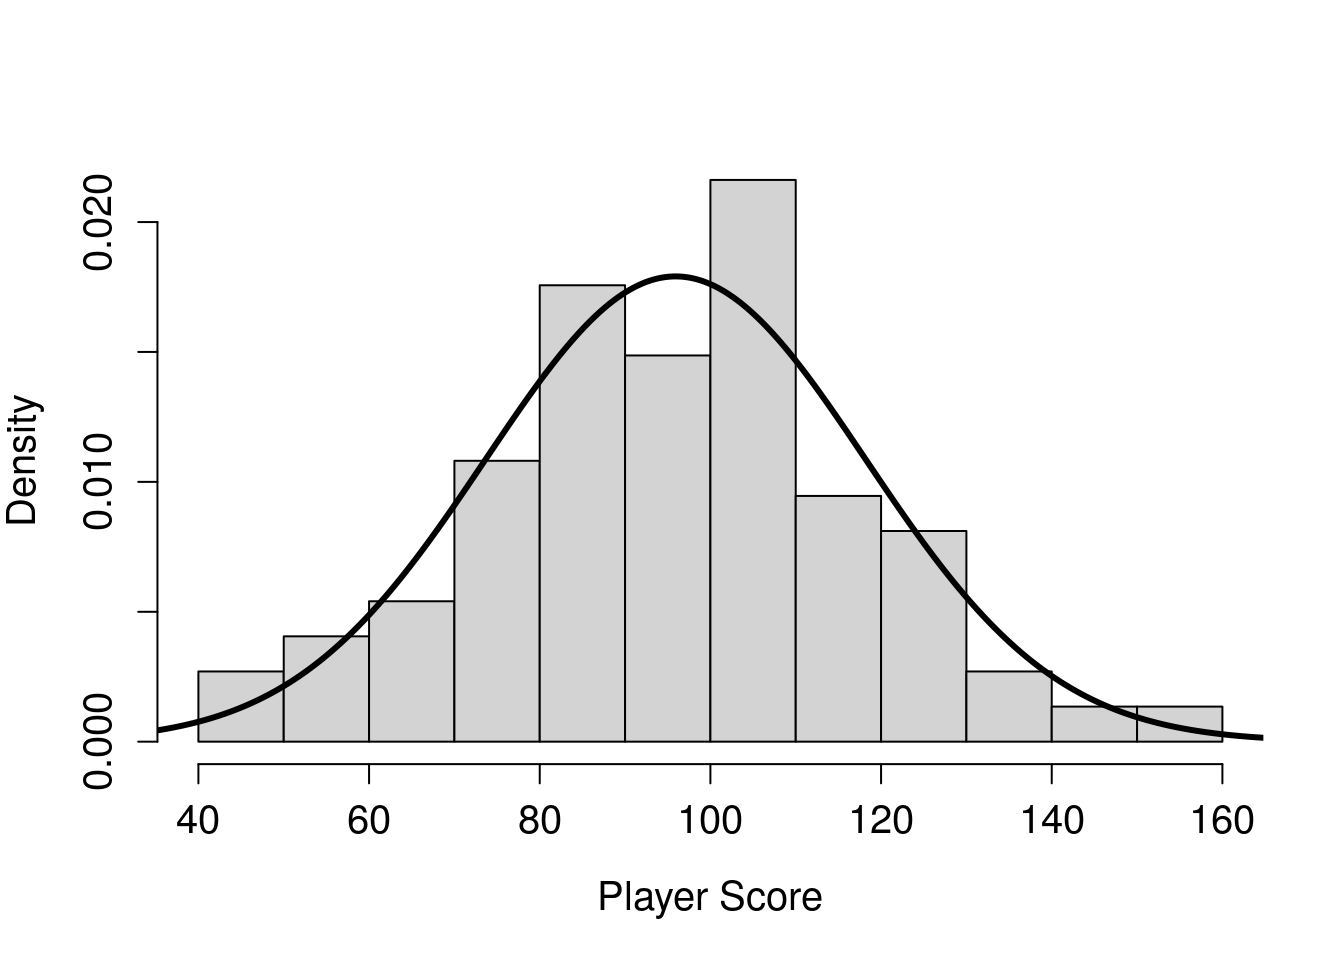
\includegraphics{bookdown-demo_files/figure-latex/unnamed-chunk-59-1} \caption{Poisson probability distributions given different rate parameter values.}\label{fig:unnamed-chunk-59}
\end{figure}

Like the binomial distribution, the Poisson distribution can also be defined mathematically\footnote{A random variable \(X\) has a Poisson distribution if and only if its probability mass function is defined by \citep{Miller2004}, \[p \left(x; \lambda \right) = \frac{\lambda^{x}e^{x}}{x!}.\] Recall from \protect\hyperlink{Chapter_1}{Chapter 1} Euler's number, \(e \approx 2.718282\), and from footnote 13 that the exclamation mark indicates a factorial. In the Poisson probability mass function, \(x\) can take any integer value greater than or equal to 0.}.
Also like the binomial distribution, probabilities in the Poisson distribution focus on \textbf{discrete} observations.
This is, probabilities are assigned to a specific number of successes in a set of trials (binomial distribution) or the number of events over time (Poisson distribution).
In both cases, the probability distribution focuses on countable numbers.
In other words, it does not make any sense to talk about the probability of a coin landing on heads 3.75 times after 10 flips, nor the probability of 2.21 runners passing by a park bench in a given minute.
The probability of either of these events happening is zero, which is why the Figures 14.5-14.7 all have spaces between the vertical bars.
These spaces indicate that values between the integers are impossible.
When observations are discrete like this, they are defined by a \emph{probability mass function}.
In the next section, we consider distributions with a continuous range of possible sample values; these distributions are defined by a \emph{probability density function}.

\hypertarget{uniform-distribution}{%
\subsection{Uniform distribution}\label{uniform-distribution}}

We now move on to continuous distributions, starting with the continuous uniform distribution.
We introduce this distribution mainly to clarify the difference between a discrete and continuous distribution.
While the uniform distribution is very important in a lot of statistical tools (notably, simulating pseudorandom numbers), it is not something that we come across much in biological or environmental science data.
The continuous uniform distribution has two parameters, \(\alpha\) and \(\beta\) \citep{Miller2004}.\footnote{A random variable \(X\) has a continuous uniform distribution if and only if its probability density function is defined by \citep{Miller2004}, \[u\left(x; \alpha, \beta\right) = \frac{1}{\beta - \alpha},\] where \(\alpha < x < \beta\), and \(u\left(x; \alpha, \beta\right) = 0\) everywhere else. The value \(x\) can take any real number.}
Values of \(\alpha\) and \(\beta\) can be any real number (not just integers).
For example, suppose that \(\alpha = 1\) and \(\beta = 2.5\).
In this case, Figure 14.8 shows the probability distribution for sampling some value \(x\).

\begin{figure}
\includegraphics{bookdown-demo_files/figure-latex/unnamed-chunk-60-1} \caption{A continuous uniform distribution in which a random variable X takes a value between 1 and 2.5.}\label{fig:unnamed-chunk-60}
\end{figure}

The height of the distribution in Figure 14.8 is \(1/(\beta - \alpha) = 1/(2.5 - 1) \approx 0.667\).
All values between 1 and 2.5 have equal probability of being sampled.

Here is a good place to point out the difference between the continuous distribution versus the discrete binomial and Poisson distributions.
From the uniform distribution of Figure 14.8, we can, theoretically, sample \emph{any} real value between 1 and 2.5 (e.g., 1.34532 or 2.21194; the sampled value can have as many decimals as our measuring device allows).
There are uncountably infinite real numbers, so it no longer makes sense to ask what is the probability of sampling a specific number.
For example, what is the probability of sampling a value of \emph{exactly} 2, rather than, say, 1.999999 or 2.000001, or something else arbitrarily close to 2?
The probability of sampling a specific number exactly is negligible.
Instead, we need to think about the probability of sampling within intervals.
For example, what is the probability of sampling a value between 1.9 and 2.1, or any value greater than 2.2?
This is the nature of probability when we consider continuous distributions.

\hypertarget{normal-distribution}{%
\subsection{Normal distribution}\label{normal-distribution}}

The last distribution, the normal distribution (also known as the ``Gaussian distribution'' or the ``bell curve'') has a special place in statistics \citep{Miller2004, Navarro2022}.
It appears in many places in the biological and environmental sciences and, partly due to the central limit theorem (see \protect\hyperlink{Chapter_15}{Chapter 15}), is fundamental to many statistical tools.
The normal distribution is continuous, just like the continuous uniform distribution from the previous section.
Unlike the uniform distribution, with the normal distribution, it is possible (at least in theory) to sample \emph{any} real value, \(-\infty < x < \infty\).
The distribution has a symmetrical, smooth bell shape (Figure 14.8), in which probability density peaks at the mean, which is also the median and mode of the distribution.
The normal distribution has two parameters, the mean (\(\mu\)) and the standard deviation (\(\sigma\)).\footnote{A random variable \(X\) has a normal distribution if and only if its probability density function is defined by \citep{Miller2004}, \[n\left(x; \mu, \sigma\right) = \frac{1}{\sigma\sqrt{2\pi}}e^{-\frac{1}{2}\left(\frac{x - \mu}{\sigma}\right)^{2}}.\] In the normal distribution, \(-\infty < x < \infty\). Note the appearance of two irrational numbers introduced back in \protect\hyperlink{Chapter_1}{Chapter 1}, \(\pi\) and \(e\).}
The mean determines where the peak of the distribution is, and the standard deviation determines the width or narrowness of the distribution.
Note that we are using \(\mu\) for the mean here instead of \(\bar{x}\), and \(\sigma\) for the standard deviation instead of \(s\), to differentiate between the \emph{population} parameters from the \emph{sample} estimates of \protect\hyperlink{Chapter_11}{Chapter 11} and \protect\hyperlink{Chapter_12}{Chapter 12}.

\begin{figure}
\includegraphics{bookdown-demo_files/figure-latex/unnamed-chunk-61-1} \caption{A standard normal probability distribution, which is defined by a mean value of 0 and a standard deviation of 1.}\label{fig:unnamed-chunk-61}
\end{figure}

The normal distribution shown in Figure 14.9 is called the \textbf{standard normal distribution}, which means that it has a mean of 0 (\(\mu = 0\)) and a standard deviation of 1 (\(\sigma = 1\)).
Note that because the standard deviation of a distribution is the square-root of the variance (see \protect\hyperlink{Chapter_12}{Chapter 12}), and \(\sqrt{1} = 1\), the variance of the standard normal distribution is also 1.
We will look at the standard normal distribution more closely in \protect\hyperlink{Chapter_15}{Chapter 15}.

\hypertarget{summary-2}{%
\section{Summary}\label{summary-2}}

This chapter has introduced probability models and different types of distributions.
It has focused on the key points that are especially important for understanding and implementing statistical techniques.
As such, a lot of details have been left out.
For example, the probability distributions considered in Section 14.4 comprise only a small number of example distributions that are relevant for biological and environmental sciences.
In \protect\hyperlink{Chapter_15}{Chapter 15}, we will get an even closer look at the normal distribution and why it is especially important.

\hypertarget{Chapter_15}{%
\chapter{The Central Limit Theorem (CLT)}\label{Chapter_15}}

The previous chapter finished by introducing the normal distribution.
This chapter focuses on the normal distribution in more detail and explains why it is so important in statistics.

\hypertarget{the-distribution-of-means-is-normal}{%
\section{The distribution of means is normal}\label{the-distribution-of-means-is-normal}}

The central limit theorem (CLT) is one of the most important theorems in statistics.
It states that if we sample values from \textbf{any} distribution and calculate the mean, as we increase our sample size \(N\), the distribution \emph{of the mean} gets closer and closer to a normal distribution \citep{Sokal1995, Miller2004, Spiegelhalter2019}.\footnote{For those interested, a mathematical proof of the CLT can be found in \citet{Miller2004}. Here we will demonstrate the CLT by simulation. As an aside, the CLT also applies to the sum of sample values, which will also have a distribution that approaches normality as \(N \to \infty\).}
This statement is busy and potentially confusing at first, partly because it refers to two separate distributions, the sampling distribution and the distribution of the sample mean.
We can take this step by step, starting with the sampling distribution.

The sampling distribution could be any of the 4 distributions introduced in \protect\hyperlink{Chapter_14}{Chapter 14} (binomial, Poisson, uniform, or normal).
Suppose that we sample the binomial distribution from Figure 14.6, the one showing the number of people out of 6 who would test positive for Covid-19 if the probability of testing positive was 0.025.
Assume that we sample a value from this distribution (i.e., a number from 0 to 6) 100 times (i.e., \(N = 100\)).
If it helps, we can imagine going to 100 different shops, all of which are occupied by 6 people.
From these 100 samples, we can calculate the sample mean \(\bar{x}\).
This would be the mean number of people in a shop who would test positive for Covid-19.
If we were just collecting data to try to estimate the mean number of people with Covid-19 in shops of 6, this is where our calculations might stop.
But here is where the second distribution becomes relevant.

Suppose that we could somehow go back out to collect \emph{another} 100 samples from 100 completely different shops.
We could then get the mean of this new sample of \(N = 100\) shops.
To differentiate, we can call the first sample mean \(\bar{x}_{1}\) and this new sample mean \(\bar{x}_{2}\).
Will \(\bar{x}_{1}\) and \(\bar{x}_{2}\) be the exact same value?
Probably not!
Since our samples are independent and random from the binomial distribution (Figure 14.6), it is almost certain that the two sample means will be at least a bit different.
We can therefore ask about the \emph{distribution} of sample means.
That is, what if we kept going back out to get more samples of 100, calculating additional sample means \(\bar{x}_{3}\), \(\bar{x}_{4}\), \(\bar{x}_{5}\), and so forth?
What would this distribution look like?
It turns out, it would be a normal distribution!

\begin{figure}
\includegraphics{bookdown-demo_files/figure-latex/unnamed-chunk-62-1} \caption{A simulated demonstration of the central limit theorem. (a) Recreation of Figure 14.6 showing the probability distribution for the number of people who have Covid-19 in a shop of 6 when the probability of testing positive is 0.025. (b) The distribution of 1000 means sampled from panel (a), where the sample size is 100.}\label{fig:unnamed-chunk-62}
\end{figure}

To demonstrate the CLT in action, Figure 15.1 shows the two distributions side-by-side.
The first (Figure 15.1a) shows the original distribution from Figure 14.6, from which samples are collected and sample means are calculated.
The second (Figure 15.1b) shows the distribution of 1000 sample means (i.e., \(\bar{x}_{1}, \bar{x}_{2}, ..., \bar{x}_{999}, \bar{x}_{1000}\)).
Each mean \(\bar{x}_{i}\) is calculated from a sample of \(N = 100\) from the distribution in Figure 15.1a.
Sampling is simulated using a random number generator on the computer (the lab practical in \protect\hyperlink{Chapter_16}{Chapter 16} shows an example of how to do this in Jamovi).

The distribution of sample means shown in Figure 15.1b is not perfectly normal.
We can try again with an even bigger sample size of \(N = 1000\), this time with a Poisson distribution where \(\lambda = 1\) in Figure 14.7.
Figure 15.2 shows this result, with the original Poisson distribution shown in Figure 15.2a, and the corresponding distribution built from 1000 sample means shown in Figure 15.2b.

\begin{figure}
\includegraphics{bookdown-demo_files/figure-latex/unnamed-chunk-63-1} \caption{A simulated demonstration of the central limit theorem. (a) Recreation of Figure 14.7 showing the probability distribution for the number of events occurring in a Poisson distribution with a rate parameter of 1. (b) The distribution of 1000 means sampled from panel (a), where the sample size is 1000.}\label{fig:unnamed-chunk-63}
\end{figure}

Finally, we can try the same approach with the continuous uniform distribution shown in Figure 14.8.
This time, we will use an even larger sample size of \(N = 10000\) to get our 1000 sample means.
The simulated result is shown in Figure 15.3.

\begin{figure}
\includegraphics{bookdown-demo_files/figure-latex/unnamed-chunk-64-1} \caption{A simulated demonstration of the central limit theorem. (a) Recreation of Figure 14.8 showing a continuous uniform distribution with a minimum of 1 and a maximum of 2.5. (b) The distribution of 1000 means sampled from panel (a), where the sample size is 10000.}\label{fig:unnamed-chunk-64}
\end{figure}

In all cases, regardless of the original sampling distribution (binomial, Poisson, or uniform), the distribution of sample \emph{means} has the shape of a normal distribution.
This normal distribution of sample means has important implications for statistical hypothesis testing.
The CLT allows us to make inferences about the means of non-normally distributed distributions \citep{Sokal1995}, to create confidence intervals around sample means, and to apply statistical hypothesis tests that would otherwise not be possible.
We will look at these statistical tools in future chapters.

\hypertarget{probability-and-z-scores}{%
\section{Probability and z-scores}\label{probability-and-z-scores}}

We can calculate the probability of sampling some range of values from the normal distribution if we know the distribution's mean (\(\mu\)) and standard deviation (\(\sigma\)).
For example, because the normal distribution is symmetric around the mean, the probability of sampling a value greater than the mean will be 0.5 (i.e., \(P(x > \mu) = 0.5\)), and so will the probability of sampling a value less than the mean (i.e., \(P(x < \mu) = 0.5\)).
Similarly, about 68.2\% of the normal distribution's probability density lies within 1 standard deviation of the mean (shaded region of Figure 15.4), which means that the probability of randomly sampling a value \(x\) that is greater than \(\mu - \sigma\) but less than \(\mu + \sigma\) is \(P(\mu - \sigma < x < \mu + \sigma) = 0.682\).

\begin{figure}
\includegraphics{bookdown-demo_files/figure-latex/unnamed-chunk-65-1} \caption{A normal distribution in which the shaded region shows the area within one standard deviation of the mean (dotted line); that is, the shaded region starts on the left at the mean minus one standard deviation, then ends at the right at the mean plus one standard deviation. This shaded area encompases 68.2 per cent of the total area under the curve.}\label{fig:unnamed-chunk-65}
\end{figure}

Remember that total probability always needs to equal 1.
This remains true whether it is the binomial distribution that we saw with the coin flipping example in \protect\hyperlink{Chapter_14}{Chapter 14}, or any other distribution.
Consequently, the area under the curve of the normal distribution (i.e., under the curved line of Figure 15.4) must equal 1.
When we say that the probability of sampling a value within 1 standard deviation of the mean is 0.682, this also means that the \emph{area} of this region under the curve equals 0.682 (i.e., the shaded area in Figure 15.4).
And, again, because the whole area under the curve sums to 1, that must mean that the unshaded area of Figure 15.4 (where \(x < \mu -\sigma\) or \(x > \mu + \sigma\)) has an area equal to \(1 - 0.682 = 0.318\).
That is, the probability of randomly sampling a value \(x\) in this region is \(P(x < \mu - \sigma \: \cup \: x > \mu + \sigma) = 0.318\), or 31.8\% (note that the \(\cup\), is just a fancy way of saying `or', in this case; technically, the \emph{union} of two sets).

We can calculate other percentages using standard deviations too \citep{Sokal1995}.
For example, about 95.4\% of the probability density in a normal distribution lies between 2 standard deviations of the mean, i.e., \(P(\mu - 2\sigma < x < \mu + 2\sigma) = 0.954\).
And about 99.6\% of the probability density in a normal distribution lies between 3 standard deviations of the mean, i.e., \(P(\mu - 3\sigma < x < \mu + 3\sigma) = 0.996\).
We could go on mapping percentages to standard deviations like this; for example, about 93.3\% of the probability density in a normal distribution is less than \(\mu + 1.5\sigma\) (i.e., less than 1.5 standard deviations greater than the mean; see Figure 15.5).

\begin{figure}
\includegraphics{bookdown-demo_files/figure-latex/unnamed-chunk-66-1} \caption{A normal distribution in which the shaded region shows the area under 1.5 standard deviations of the mean (dotted line). This shaded area encompases about 93.3 per cent of the total area under the curve.}\label{fig:unnamed-chunk-66}
\end{figure}

Notice that there are no numbers on the x-axes of Figure 15.4 or 15.5.
This is deliberate; the relationship between standard deviations and probability density applies regardless of the scale.
We could have a mean of \(\mu = 100\) and standard deviation of \(\sigma = 4\), or \(\mu = -12\) and \(\sigma = 0.34\).
It does not matter.
Nevertheless, it would be very useful if we could work with some standard values of \(x\) when working out probabilities.
This is where the standard normal distribution, first introduced in \protect\hyperlink{Chapter_14}{Chapter 14}, becomes relevant.
Recall that the standard normal distribution has a mean of \(\mu = 0\) and a standard deviation (and variance) of \(\sigma = 1\).
With these standard values of \(\mu\) and \(\sigma\), we can start actually putting numbers on the x-axis and relating them to probabilities.
We call these numbers \textbf{standard normal deviates}, or \textbf{z-scores} (Figure 15.6).

\begin{figure}
\includegraphics{bookdown-demo_files/figure-latex/unnamed-chunk-67-1} \caption{A standard normal probability distribution with z-scores shown on the x-axis.}\label{fig:unnamed-chunk-67}
\end{figure}

What z-scores allow us to do is map probabilities to deviations from the mean of a standard normal distribution (hence `standard normal deviates').
We can say, e.g., that about 95\% of the probability density lies between \(z = -1.96\) and \(z = 1.96\), or that about 99\% lies between \(z = -2.58\) and \(z = 2.58\) (this will become relevant later).
It is important to get a good sense of what this means, so we have written an interactive application (\href{https://bradduthie.shinyapps.io/zandp/}{click here}) that visually shows how probability density changes with changing z-score.

\begin{quote}
\href{https://bradduthie.shinyapps.io/zandp/}{Click here} for an interactive application to visualise z-scores
\end{quote}

Of course, most variables that we measure in the biological and environmental sciences will not fit the standard normal distribution.
Almost all variables will have a different mean and standard deviation, even if they are normally distributed.
Nevertheless, we can translate any normally distributed variable into a standard normal distribution by subtracting its mean and dividing by its standard deviation.
We can see what this looks like visually in Figure 15.7.

\begin{figure}
\includegraphics{bookdown-demo_files/figure-latex/unnamed-chunk-68-1} \caption{A visual representation of what happens when we subtract the sample mean from a dataset, then divide by its standard deviation. (a) A histogram (grey bars) show 10000 normally distributed values with a mean of 5 and a standard deviation of 2; the curved dotted line shows the standard normal distribution with a mean of 0 and standard deviation of 1. (b) Histogram after subtracting 5, then dividing by 2, from all values shown in panel (a).}\label{fig:unnamed-chunk-68}
\end{figure}

In Figure 15.7a, we see the standard normal distribution curve represented by the dotted line, centered at \(\mu = 0\) and with a standard deviation of \(\sigma = 1\).
To the right of this normal distribution we have 10000 values randomly sampled from a normal distribution with a mean of 5 and a standard deviation of 2 (note that the histogram peaks around 5 and is wider than the standard normal distribution because the standard deviation is higher).
After subtracting 5 from all of the values in the histogram of Figure 15.7a, then dividing by 2, the data fit nicely within the standard normal curve, as shown in Figure 15.7b.
By doing this transformation on the original dataset, z-scores can now be used with the data.
Mathematically, here is how the calculation is made,

\[z = \frac{x - \mu}{\sigma}.\]

For example, if we had a value of \(x = 9.1\) in our simulated dataset, in which \(\mu = 5\) and \(\sigma = 2\), then we could calculate \(z = (9.1 - 5) / 2 = 2.05\).
Since we almost never know what the true population mean (\(\mu\)) and standard deviation (\(\sigma\)) are, we usually need to use the estimates made from our sample,

\[z = \frac{x - \bar{x}}{s}.\]

We could then use a statistical program such as Jamovi, our \href{https://bradduthie.shinyapps.io/zandp/}{interactive application}, or an old-fashioned z-table\footnote{Before the widespread availability of computers, which can easily be used to calculate probability densities on a normal distribution, the way to map \(z\) scores to probabilities was using a \href{https://www.z-table.com/}{z table}. The table would have rows and columns mapping to different \(z\) values, which could be used to find the appropriate probability densities. Such tables would be used for many different distributions, not just the normal distribution. The text \citet{Sokal1995} comes with a nearly 200 page supplemental book that is just statistical tables. These tables are more or less obsolete nowadays, but some people still use them.} to find that only about 2\% of values are expected to be higher than \(x = 9.1\) in our original dataset.
These z scores will become especially useful for calculating confidence intervals in \protect\hyperlink{Chapter_17}{Chapter 17}.
They can also be useful for comparing values from variables or statistics measured on different scales \citep{Sokal1995, Cheadle2003, Adams2016}.

\hypertarget{Chapter_16}{%
\chapter{\texorpdfstring{\emph{Practical}. Probability and simulation}{Practical. Probability and simulation}}\label{Chapter_16}}

This practical focuses on applying the concepts from \protect\hyperlink{Chapter_14}{Chapter 14} and \protect\hyperlink{Chapter_15}{Chapter 15} in Jamovi.
There will be 3 exercises.

\begin{enumerate}
\def\labelenumi{\arabic{enumi}.}
\tightlist
\item
  Calculating probabilities from a dataset.
\item
  Calculating probabilities from a normal distribution.
\item
  Demonstrating the central limit theorem (CLT).
\end{enumerate}

To complete exercises 2 and 3, we will need to download and install two new Jamovi modules.
Jamovi modules are add-ons that make it possible to run specialised statistical tools inside Jamovi.
These tools are written by a community of statisticians, scientists, and educators and listed in the \href{https://www.jamovi.org/library.html}{Jamovi library}.
Like Jamovi, these tools are open source and free to use.

The dataset for this practical is something a bit different.
It comes from the \href{https://www.thebeaconproject.net/}{Beacon Project}, which is an interdisciplinary scientific research programme led by \href{https://www.stir.ac.uk/people/256518}{Dr Isabel Jones} at the University of Stirling.
This project focuses on large hydropower dams as a way to understand the trade-offs between different United Nations \href{https://sdgs.un.org/goals}{Sustainable Development Goals}.
It addresses challenging questions about environmental justice, biodiversity, and sustainable development.\\
The project works with people affected, and sometimes displaced, by dam construction in Brazil, Kazakhstan, India, USA, and the UK.
Part of this project involves the use of mobile games to investigate how people make decisions about sustainable development.

\begin{figure}
\includegraphics[width=0.8\linewidth]{img/power_up} \caption{Welcome screen of the mobile game Power Up!}\label{fig:unnamed-chunk-69}
\end{figure}

The game ``Power Up!'' is freely available as an \href{https://play.google.com/store/apps/details?id=com.hyperluminal.stirlinguniversity.sustainabledevelopmentgame}{Android} and \href{https://apps.apple.com/gb/app/power-up/id1585634888}{iPhone} app (Figure 16.1).
Data are collected from players' decisions and used to investigate social-ecological questions.
We will use the \href{https://raw.githubusercontent.com/bradduthie/SCIU4T4/main/data/power_up.csv}{power\_up} dataset in exercises 1 and 2 (right click and ``Save Link As\ldots{}'').
To get started, first download the \href{https://raw.githubusercontent.com/bradduthie/SCIU4T4/main/data/power_up.csv}{power\_up} dataset and open it in Jamovi.
Note that these data are already in a tidy format, so we do not need to do any reorganising.
The dataset includes columns for each player's ID, the OS that they use, the dam size that they decided to build in the game, their in-game investment in Biodiversity, Community, and Energy, and their final Score.

\hypertarget{probabilities-from-a-dataset}{%
\section{Probabilities from a dataset}\label{probabilities-from-a-dataset}}

Suppose that we want to estimate the probability that a new Power Up! game player will be an Android user.
To estimate this probability, we can use the proportion of players in the dataset who are Android users.
To get this proportion, we need to divide the number of Android users by the total number of players,

\[P(Android) = \frac{Number\:of\:Android\:users}{Number\:of\:players}.\]

In Jamovi, you could figure this out the long way by counting up the number of rows with `Android' in the second column, then dividing by the total number of rows.
But there is an easier way, which is faster and less prone to human error than manually tallying up items.
To do this, go to the Analyses tab in Jamovi and navigate to Exploration, then Descriptives.
Place the `OS' variable in to the `Variables' box.
Next, find the check box called `Frequency tables' just under the `Split by' box and above the `Statistics' drop down tab.
Check this box to get a table of frequencies for Android versus iPhone users.

\begin{figure}
\includegraphics[width=1\linewidth]{img/jamovi_power_up_frequencies} \caption{Jamovi Descriptives toolbar showing the OS column from the Power Up! dataset selected. The 'Frequency tables' checkbox builds a table of counts and percentages.}\label{fig:unnamed-chunk-70}
\end{figure}

The table of frequencies shown in Figure 16.2 includes counts of Android versus iPhone users.
We can see that 56 of the 74 total game players use Android, while 18 players use iPhone.
To get the proportion of Android users, we could divide 56 by 74 to get 0.7567568.
Similarly, for the proportion of iPhone users, we could calculate 18 / 74 = 0.2432432.
But Jamovi already does this for us, with a bit of rounding.
The second column of the Frequencies table gives us these proportions, but expressed as a percentage.
The percentage of Android users is 75.7\%, and the percentage of iPhone users is 24.3\%.
Percentages are out of a total of 100, so to get back to the proportions, we can just divide by 100\%, 75.7 / 100 = 0.757 for Android and 24.3 / 100 = 0.243 for iPhone.
To answer the original question, our best estimate of the probability that a new Power Up! game player will be an Android user is therefore 0.757.

Next, use the same procedure to find the probability that a game player will make a small, medium, and large size dam.
Now, fill in Table 16.1 with counts, percentage, and the estimated probability of a player selecting a small, medium, or large dam.

\begin{longtable}[]{@{}llll@{}}
\caption{Statistics of Power Up! decisions for dam size.}\tabularnewline
\toprule
Dam size & Counts & Percentage & Estimated Probability \\
\midrule
\endfirsthead
\toprule
Dam size & Counts & Percentage & Estimated Probability \\
\midrule
\endhead
Small & & & \\
Medium & & & \\
Large & & & \\
\bottomrule
\end{longtable}

We can use these estimated probabilities of small, medium, and large dam size selection to predict what will happen in future games.
Suppose that a new player decides to play the game.
What is the probability that this player chooses a small \textbf{or} a large dam?

\(P(small\:or\:large) =\) \_\_\_\_\_\_\_\_\_\_\_\_\_\_\_\_\_\_\_\_\_\_\_\_\_\_

Now suppose that 3 new players arrive and decide to play the game.
What is the probability that all 3 of these new players choose a large dam?

\(P(3\:large) =\) \_\_\_\_\_\_\_\_\_\_\_\_\_\_\_\_\_\_\_\_\_\_\_\_\_\_

What is the probability that the first player chooses a small dam, the second player chooses a medium dam, and the third player chooses a large dam?

\(P(Player\:1 = small,Player\:2 = \:medium,Player\:3 = large) =\) \_\_\_\_\_\_\_\_\_\_\_

Now consider a slightly different type of question.
Instead of trying to predict the probability of new player decisions, we will focus on sampling from the existing power up dataset.
Imagine that you randomly choose one of the 74 players with equal probability (i.e., every player is equally likely to be chosen).
What is the probability that you choose player 20?

\(P(Player\:20) =\) \_\_\_\_\_\_\_\_\_\_\_\_\_\_\_\_\_\_\_\_\_\_\_\_\_\_

What is the probability that you choose player 20, \emph{then} choose a different player with a large dam?
As a hint, remember that you are now sampling \emph{without replacement}.
The second choice cannot be player 20 again, so the probability of choosing a player with a large dam has changed from the estimated probability in Table 16.1.

\(P(Player\:20,\:Large) =\) \_\_\_\_\_\_\_\_\_\_\_\_\_\_\_\_\_\_\_\_\_\_\_\_\_\_

Now we can use the Descriptives tool in Jamovi to ask a slightly different question with the data.
Suppose that we wanted to estimate the probability that an Android user will choose a large dam.
We could multiply the proportion of Android users times the proportion of players who choose a large dam (i.e., find the probability of Android \emph{and} large dam).
But this assumes that the two characteristics are independent (i.e., that Android users are not more or less likely than iPhone users to build large dams).
To estimate the probability that a player chooses a large dam \emph{given} that they are using Android, we can keep Dam\_size in the Variables box, but now put OS in the `Split by' box.
Figure 16.3 shows the output of Jamovi.
A new frequency table breaks down dam choice for each OS.

\begin{figure}
\includegraphics[width=1\linewidth]{img/jamovi_power_up_frequencies2} \caption{Jamovi Descriptives toolbar showing the dam size column from the Power Up! dataset selected as a variable split by OS. The 'Frequency tables' checkbox builds a table of counts for small, medium, and large dam size broken down by Android versus iPhone OS.}\label{fig:unnamed-chunk-71}
\end{figure}

To get the proportion of Android users who choose to build a large dam, we just need to divide the number of Android users who chose the large dam size by the total number of Android users (i.e., sum of the first column in the Frequencies table; Figure 16.3).
Note that the vertical bar, \(|\), in the equation below just means `given' (or, rather, `conditional up', so the number of players that chose a large dam \emph{given} that they are Android users),

\[P(Large | Android) = \frac{Number\:of\:Android\:users\:choosing\:large\:dam}{Number\:of\:Android\:users}.\]

Now, recreate the table in Figure 16.3 and estimate the probability that an Android user will choose to build a large dam,

\(P(Large | Android) =\) \_\_\_\_\_\_\_\_\_\_\_\_\_\_\_\_\_\_\_\_\_\_\_\_\_\_

Is \(P(Large | Android)\) much different from the probability that \emph{any} player chooses a large dam, as calculated in Table 16.1? Do you think that the difference is significant?

\begin{verbatim}






\end{verbatim}

Next, we will move on to calculating probabilities from a normal distribution.

\hypertarget{probabilities-from-a-normal-distribution}{%
\section{Probabilities from a normal distribution}\label{probabilities-from-a-normal-distribution}}

In the example of the first exercise, we looked at OS and dam size choice.
Players only use Android or iPhone, and they could only choose one of three sizes of dam.
For these nominal variables, estimating the probability of a particular discrete outcome (e.g., Android versus iPhone) was just a matter of dividing counts.
But we cannot use the same approach for calculating probabilities from continuous data.
Consider, for example, the final score for each player in the column `Score'.
Because of how the game was designed, Score can potentially be any real number, although most scores are somewhere around 100.
We can use a histogram to see the distribution of player scores (Figure 16.4).

\begin{figure}
\includegraphics[width=1\linewidth]{bookdown-demo_files/figure-latex/unnamed-chunk-72-1} \caption{Distribution of player scores in the game Power Up!}\label{fig:unnamed-chunk-72}
\end{figure}

In this case, it does not really make sense to ask what the probability is of a particular score.
If the score can take \emph{any} real value, out to as many decimals as we want, then what is the probability of a score being \emph{exactly} 94.97 (i.e., 94.97 with infinite zeros after it, \(94.9700000\bar{0}\))?
The probability is infinitesimal, i.e., basically zero, because there are an infinite number of real numbers.
Consequently, we are not really interested in the probabilities of specific values of continuous data.
Instead, we want to focus on intervals.
For example, what is the probability that a player scores higher than 120?
What is the probability that a player scores lower than 100?
What is the probability that a player scores between 100 and 120?

Take another look at Figure 16.4, then take a guess at each of these probabilities.
As a hint, the y-axis of this histogram is showing density instead of frequency.
What this means is that the total grey area (i.e., the histogram bars) sums to 1.
Guessing the probability that a player scores higher than 120 is the same as guessing the proportion of grey space in the highest 4 bars of Figure 16.4 (i.e., grey space \textgreater120).

\(P(Score>120) =\) \_\_\_\_\_\_\_\_\_\_\_\_\_\_\_\_\_\_\_\_\_\_\_\_\_\_

\(P(Score<100) =\) \_\_\_\_\_\_\_\_\_\_\_\_\_\_\_\_\_\_\_\_\_\_\_\_\_\_

\(P(100<Score<120) =\) \_\_\_\_\_\_\_\_\_\_\_\_\_\_\_\_\_\_\_\_\_\_\_\_\_\_

Trying to do this by looking at a histogram is not easy, and it is really not the best way to get the above probabilities.
We can get much better estimates using Jamovi, but we need to make an assumption about the distribution of Player Score.
Specifically, we need to assume that the distribution of Player Score has a specific shape.
More technically, we must assume a specific probability density function that we can use to mathematically calculate probabilities of different ranges of player scores.
Inspecting Figure 16.4, Player Score appears to be normally distributed.
In other words, the shape of Player Score distribution appears to be normal, or `Gaussian'.
If we are willing to assume this, then we can calculate probabilities using its mean and standard deviation.
Use Jamovi to find the mean and the standard deviation of player score (note, we can just say that score is unitless, so no need to include units).

Mean score: \_\_\_\_\_\_\_\_\_\_\_\_\_\_\_\_\_\_\_\_\_\_\_\_\_\_

Standard deviation score: \_\_\_\_\_\_\_\_\_\_\_\_\_\_\_\_\_\_\_\_\_\_\_\_\_\_

We will assume that the \emph{sample} of scores shown in Figure 16.4 came from a \emph{population} that is normally distributed with the mean and standard deviation that you wrote above (recall sample versus population from \protect\hyperlink{Chapter_4}{Chapter 4}).
We can overlay this distribution on the histogram above using a curved line (Figure 16.5).

\begin{figure}
\includegraphics[width=1\linewidth]{bookdown-demo_files/figure-latex/unnamed-chunk-73-1} \caption{Distribution of player scores in the game Power Up! shown in histogram bars. The overlaid curve shows the probability density function for a normal distribution that has the same mean and standard deviation as the sample described by the histogram.}\label{fig:unnamed-chunk-73}
\end{figure}

We can interpret the area under the curve in the same way that we interpret the area in the grey bars.
As mentioned earlier, the total area of the histogram bars must sum to 1.
The total area under the curve must also sum to 1.
Both represent the probability of different ranges of player scores.
Notice that the normal distribution is not a perfect match for the histogram bars.
For example, the middle bar of values illustrating scores between 90 and 100 appears to be a bit low compared to a perfect normal distribution, and there are more scores between 40 and 50 than we might expect.
Nevertheless, the two distributions broadly overlap, so we might be willing to assume that the player scores represented in the histogram bars are sampled from the population described by the curve.

Because the curve relating player score to probability density is described by an equation (see \protect\hyperlink{Chapter_14}{Chapter 14}), we can use that equation to make inferences about the probabilities of different ranges of scores.
The simplest example is the mean of the distribution.
Because the normal distribution is symmetric, the area to the left of the mean must be the same as the area to the right of the mean.
And since the whole area under the curve must sum to 1, we can conclude that the probability of sampling a player score that is less than the mean is 1/2, and the probability of sampling a player score greater than the mean is also 1/2.
Traditionally, we would need to do some maths to get other player score probabilities, but Jamovi can do this much more easily.

To get Jamovi to calculate probabilities from a normal distribution, we need to go to the Modules option and download a new module (Figure 16.6).

\begin{figure}
\includegraphics[width=1\linewidth]{img/jamovi_toolbar_modules} \caption{Jamovi tool bar, which includes an option for downloading new Modules (right hand side)}\label{fig:unnamed-chunk-74}
\end{figure}

Click on the `Modules' button, and select the first option called `jamovi library' from the pull-down menu.
From the `Available' tab, scroll down until you find the Module called `distrACTION - Quantiles and Probabilities of Continuous and Discrete Distributions' \citep{Rihs2018}.
Click the `Install' button to install it into Jamovi.
A new button in the toolbar called `distrACTION' should become visible (Figure 16.7).

\begin{figure}
\includegraphics[width=1\linewidth]{img/jamovi_toolbar_modules_distrACTION} \caption{Jamovi tool bar, which includes an added module called distrACTION.}\label{fig:unnamed-chunk-75}
\end{figure}

If the module is not there after installation, then it should be possible to find by again going to Modules and selecting distrACTION from the pulldown menu.
Click on the module and choose `Normal Distribution' from the pulldown menu.
Next, we can see a box for the mean and standard deviation (SD) under the `Parameters' subtitle in bold.
Put the mean and the standard deviation calculated from above into these boxes.
In the panel on the right, Jamovi will produce the same normal distribution that is in Figure 16.5 (note that the axes might be scaled a bit differently).

Given this normal distribution, we can compute the probability that a player scores less than x1 = 80 by checking the box `Compute probability', which is located just under `Function' (Figure 16.8).
We can then select the first radio button to find the probability that a randomly sampled value X from this distribution is less than x1, \(P(X \leq x1)\).
Notice in the panel on the right that the probability is given as \(P = 0.238\).
This is also represented in the plot of the normal distribution, with the same proportion in the lower part of the distribution shaded (\(P = 0.238\), i.e., about 23.8 per cent).

\begin{figure}
\includegraphics[width=0.8\linewidth]{img/jamovi_normal_distribution} \caption{Jamovi options for the distrACTION module for computing probability for a given normal distribution. The example shown here calculates the probability that a value sampled from the normal distribution of interest is less than 80.}\label{fig:unnamed-chunk-76}
\end{figure}

To find the probability that a value is greater than 80, we could subtract our answer of 0.238 from 1, 1 - 0.238 = 0.762 (remember that the total area under the normal curve equals 1, so the shaded plus the unshaded region must also equal 1; hence, 1 minus the shaded region gives us the unshaded region).
We could also just select the second radio button for \(P(X \geq x1)\).
Give this a try, and notice that the shaded and unshaded regions have flipped in the plot, and we get our answer in the table of 0.762.

Finally, to compute the probability of an interval, we can check the third radio button and set x2 in the bottom box (Figure 16.8).
For example, to see the probability of a score between 80 and 120, we can choose select \(P(x1 \leq X \leq x2)\), then set \(x2 = 120\) in the bottom box.
Notice where the shaded area is in the newly drawn plot.
What is the probability of a player getting a score between 80 and 120?

\(P(80 \leq X \leq 120)\) = \_\_\_\_\_\_\_\_\_\_\_\_\_\_\_\_\_\_\_\_\_\_\_\_\_\_

What is the probability of a player getting a score greater than 130?

\(P(X \geq 130)\) = \_\_\_\_\_\_\_\_\_\_\_\_\_\_\_\_\_\_\_\_\_\_\_\_\_\_

Now try the following probabilities for different scores.

\(P(X \geq 120)\) = \_\_\_\_\_\_\_\_\_\_\_\_\_\_\_\_\_\_\_\_\_\_\_\_\_\_

\(P(X \leq 100)\) = \_\_\_\_\_\_\_\_\_\_\_\_\_\_\_\_\_\_\_\_\_\_\_\_\_\_

\(P(100 \leq X \leq 120)\) = \_\_\_\_\_\_\_\_\_\_\_\_\_\_\_\_\_\_\_\_\_\_\_\_\_\_

Note, these last 3 were the same intervals that you guessed using the histogram.
How close was your original guess to the calculations above?

\begin{verbatim}






\end{verbatim}

One last one.
What is the probability of a player getting a score lower than 70 or higher than 130?

\(P(X \leq 70 \: \cup \: X \geq 130)\) = \_\_\_\_\_\_\_\_\_\_\_\_\_\_\_\_\_\_\_\_\_\_\_\_\_\_

There is more than one way to figure this last one out.
How did you do it, and what was your reasoning?

\begin{verbatim}






\end{verbatim}

We will now move on to the central limit theorem.

\hypertarget{central-limit-theorem}{%
\section{Central limit theorem}\label{central-limit-theorem}}

To demonstrate the central limit theorem, we need to download and install another module in Jamovi.
This time, go to `Modules', and from the `Available' tab, scroll down until you find `Rj' in the Jamovi library.
Install `Rj', then a new button `R' should become available in the toolbar.
This will allow us to run a bit of script using the coding language R.
We will work with R a bit more in future practicals, but for now you will not need to do anymore than copying and pasting.
For now, click on the new `R' button in the toolbar and select `Rj Editor' from the pulldown menu.
You will see an open editor; this is where the code will go.
If it has some code in it already (e.g., \texttt{\#\ summary(data{[}1:3{]})}), just delete it so that we can start with a clean slate.
Copy and paste the following lines into the Rjeditor.

\begin{Shaded}
\begin{Highlighting}[]
\NormalTok{v1  }\OtherTok{\textless{}{-}} \FunctionTok{runif}\NormalTok{(}\AttributeTok{n =} \DecValTok{200}\NormalTok{, }\AttributeTok{min =} \DecValTok{0}\NormalTok{, }\AttributeTok{max =} \DecValTok{100}\NormalTok{);}
\NormalTok{v2  }\OtherTok{\textless{}{-}} \FunctionTok{runif}\NormalTok{(}\AttributeTok{n =} \DecValTok{200}\NormalTok{, }\AttributeTok{min =} \DecValTok{0}\NormalTok{, }\AttributeTok{max =} \DecValTok{100}\NormalTok{);}
\NormalTok{v3  }\OtherTok{\textless{}{-}} \FunctionTok{runif}\NormalTok{(}\AttributeTok{n =} \DecValTok{200}\NormalTok{, }\AttributeTok{min =} \DecValTok{0}\NormalTok{, }\AttributeTok{max =} \DecValTok{100}\NormalTok{);}
\NormalTok{v4  }\OtherTok{\textless{}{-}} \FunctionTok{runif}\NormalTok{(}\AttributeTok{n =} \DecValTok{200}\NormalTok{, }\AttributeTok{min =} \DecValTok{0}\NormalTok{, }\AttributeTok{max =} \DecValTok{100}\NormalTok{);}
\NormalTok{v5  }\OtherTok{\textless{}{-}} \FunctionTok{runif}\NormalTok{(}\AttributeTok{n =} \DecValTok{200}\NormalTok{, }\AttributeTok{min =} \DecValTok{0}\NormalTok{, }\AttributeTok{max =} \DecValTok{100}\NormalTok{);}
\NormalTok{v6  }\OtherTok{\textless{}{-}} \FunctionTok{runif}\NormalTok{(}\AttributeTok{n =} \DecValTok{200}\NormalTok{, }\AttributeTok{min =} \DecValTok{0}\NormalTok{, }\AttributeTok{max =} \DecValTok{100}\NormalTok{);}
\NormalTok{v7  }\OtherTok{\textless{}{-}} \FunctionTok{runif}\NormalTok{(}\AttributeTok{n =} \DecValTok{200}\NormalTok{, }\AttributeTok{min =} \DecValTok{0}\NormalTok{, }\AttributeTok{max =} \DecValTok{100}\NormalTok{);}
\NormalTok{v8  }\OtherTok{\textless{}{-}} \FunctionTok{runif}\NormalTok{(}\AttributeTok{n =} \DecValTok{200}\NormalTok{, }\AttributeTok{min =} \DecValTok{0}\NormalTok{, }\AttributeTok{max =} \DecValTok{100}\NormalTok{);}
\NormalTok{v9  }\OtherTok{\textless{}{-}} \FunctionTok{runif}\NormalTok{(}\AttributeTok{n =} \DecValTok{200}\NormalTok{, }\AttributeTok{min =} \DecValTok{0}\NormalTok{, }\AttributeTok{max =} \DecValTok{100}\NormalTok{);}
\NormalTok{v10 }\OtherTok{\textless{}{-}} \FunctionTok{runif}\NormalTok{(}\AttributeTok{n =} \DecValTok{200}\NormalTok{, }\AttributeTok{min =} \DecValTok{0}\NormalTok{, }\AttributeTok{max =} \DecValTok{100}\NormalTok{);}
\NormalTok{v11 }\OtherTok{\textless{}{-}} \FunctionTok{runif}\NormalTok{(}\AttributeTok{n =} \DecValTok{200}\NormalTok{, }\AttributeTok{min =} \DecValTok{0}\NormalTok{, }\AttributeTok{max =} \DecValTok{100}\NormalTok{);}
\NormalTok{v12 }\OtherTok{\textless{}{-}} \FunctionTok{runif}\NormalTok{(}\AttributeTok{n =} \DecValTok{200}\NormalTok{, }\AttributeTok{min =} \DecValTok{0}\NormalTok{, }\AttributeTok{max =} \DecValTok{100}\NormalTok{);}
\NormalTok{v13 }\OtherTok{\textless{}{-}} \FunctionTok{runif}\NormalTok{(}\AttributeTok{n =} \DecValTok{200}\NormalTok{, }\AttributeTok{min =} \DecValTok{0}\NormalTok{, }\AttributeTok{max =} \DecValTok{100}\NormalTok{);}
\NormalTok{v14 }\OtherTok{\textless{}{-}} \FunctionTok{runif}\NormalTok{(}\AttributeTok{n =} \DecValTok{200}\NormalTok{, }\AttributeTok{min =} \DecValTok{0}\NormalTok{, }\AttributeTok{max =} \DecValTok{100}\NormalTok{);}
\NormalTok{v15 }\OtherTok{\textless{}{-}} \FunctionTok{runif}\NormalTok{(}\AttributeTok{n =} \DecValTok{200}\NormalTok{, }\AttributeTok{min =} \DecValTok{0}\NormalTok{, }\AttributeTok{max =} \DecValTok{100}\NormalTok{);}
\NormalTok{v16 }\OtherTok{\textless{}{-}} \FunctionTok{runif}\NormalTok{(}\AttributeTok{n =} \DecValTok{200}\NormalTok{, }\AttributeTok{min =} \DecValTok{0}\NormalTok{, }\AttributeTok{max =} \DecValTok{100}\NormalTok{);}
\NormalTok{v17 }\OtherTok{\textless{}{-}} \FunctionTok{runif}\NormalTok{(}\AttributeTok{n =} \DecValTok{200}\NormalTok{, }\AttributeTok{min =} \DecValTok{0}\NormalTok{, }\AttributeTok{max =} \DecValTok{100}\NormalTok{);}
\NormalTok{v18 }\OtherTok{\textless{}{-}} \FunctionTok{runif}\NormalTok{(}\AttributeTok{n =} \DecValTok{200}\NormalTok{, }\AttributeTok{min =} \DecValTok{0}\NormalTok{, }\AttributeTok{max =} \DecValTok{100}\NormalTok{);}
\NormalTok{v19 }\OtherTok{\textless{}{-}} \FunctionTok{runif}\NormalTok{(}\AttributeTok{n =} \DecValTok{200}\NormalTok{, }\AttributeTok{min =} \DecValTok{0}\NormalTok{, }\AttributeTok{max =} \DecValTok{100}\NormalTok{);}
\NormalTok{v20 }\OtherTok{\textless{}{-}} \FunctionTok{runif}\NormalTok{(}\AttributeTok{n =} \DecValTok{200}\NormalTok{, }\AttributeTok{min =} \DecValTok{0}\NormalTok{, }\AttributeTok{max =} \DecValTok{100}\NormalTok{);}
\NormalTok{v21 }\OtherTok{\textless{}{-}} \FunctionTok{runif}\NormalTok{(}\AttributeTok{n =} \DecValTok{200}\NormalTok{, }\AttributeTok{min =} \DecValTok{0}\NormalTok{, }\AttributeTok{max =} \DecValTok{100}\NormalTok{);}
\NormalTok{v22 }\OtherTok{\textless{}{-}} \FunctionTok{runif}\NormalTok{(}\AttributeTok{n =} \DecValTok{200}\NormalTok{, }\AttributeTok{min =} \DecValTok{0}\NormalTok{, }\AttributeTok{max =} \DecValTok{100}\NormalTok{);}
\NormalTok{v23 }\OtherTok{\textless{}{-}} \FunctionTok{runif}\NormalTok{(}\AttributeTok{n =} \DecValTok{200}\NormalTok{, }\AttributeTok{min =} \DecValTok{0}\NormalTok{, }\AttributeTok{max =} \DecValTok{100}\NormalTok{);}
\NormalTok{v24 }\OtherTok{\textless{}{-}} \FunctionTok{runif}\NormalTok{(}\AttributeTok{n =} \DecValTok{200}\NormalTok{, }\AttributeTok{min =} \DecValTok{0}\NormalTok{, }\AttributeTok{max =} \DecValTok{100}\NormalTok{);}
\NormalTok{v25 }\OtherTok{\textless{}{-}} \FunctionTok{runif}\NormalTok{(}\AttributeTok{n =} \DecValTok{200}\NormalTok{, }\AttributeTok{min =} \DecValTok{0}\NormalTok{, }\AttributeTok{max =} \DecValTok{100}\NormalTok{);}
\NormalTok{v26 }\OtherTok{\textless{}{-}} \FunctionTok{runif}\NormalTok{(}\AttributeTok{n =} \DecValTok{200}\NormalTok{, }\AttributeTok{min =} \DecValTok{0}\NormalTok{, }\AttributeTok{max =} \DecValTok{100}\NormalTok{);}
\NormalTok{v27 }\OtherTok{\textless{}{-}} \FunctionTok{runif}\NormalTok{(}\AttributeTok{n =} \DecValTok{200}\NormalTok{, }\AttributeTok{min =} \DecValTok{0}\NormalTok{, }\AttributeTok{max =} \DecValTok{100}\NormalTok{);}
\NormalTok{v28 }\OtherTok{\textless{}{-}} \FunctionTok{runif}\NormalTok{(}\AttributeTok{n =} \DecValTok{200}\NormalTok{, }\AttributeTok{min =} \DecValTok{0}\NormalTok{, }\AttributeTok{max =} \DecValTok{100}\NormalTok{);}
\NormalTok{v29 }\OtherTok{\textless{}{-}} \FunctionTok{runif}\NormalTok{(}\AttributeTok{n =} \DecValTok{200}\NormalTok{, }\AttributeTok{min =} \DecValTok{0}\NormalTok{, }\AttributeTok{max =} \DecValTok{100}\NormalTok{);}
\NormalTok{v30 }\OtherTok{\textless{}{-}} \FunctionTok{runif}\NormalTok{(}\AttributeTok{n =} \DecValTok{200}\NormalTok{, }\AttributeTok{min =} \DecValTok{0}\NormalTok{, }\AttributeTok{max =} \DecValTok{100}\NormalTok{);}
\NormalTok{v31 }\OtherTok{\textless{}{-}} \FunctionTok{runif}\NormalTok{(}\AttributeTok{n =} \DecValTok{200}\NormalTok{, }\AttributeTok{min =} \DecValTok{0}\NormalTok{, }\AttributeTok{max =} \DecValTok{100}\NormalTok{);}
\NormalTok{v32 }\OtherTok{\textless{}{-}} \FunctionTok{runif}\NormalTok{(}\AttributeTok{n =} \DecValTok{200}\NormalTok{, }\AttributeTok{min =} \DecValTok{0}\NormalTok{, }\AttributeTok{max =} \DecValTok{100}\NormalTok{);}
\NormalTok{v33 }\OtherTok{\textless{}{-}} \FunctionTok{runif}\NormalTok{(}\AttributeTok{n =} \DecValTok{200}\NormalTok{, }\AttributeTok{min =} \DecValTok{0}\NormalTok{, }\AttributeTok{max =} \DecValTok{100}\NormalTok{);}
\NormalTok{v34 }\OtherTok{\textless{}{-}} \FunctionTok{runif}\NormalTok{(}\AttributeTok{n =} \DecValTok{200}\NormalTok{, }\AttributeTok{min =} \DecValTok{0}\NormalTok{, }\AttributeTok{max =} \DecValTok{100}\NormalTok{);}
\NormalTok{v35 }\OtherTok{\textless{}{-}} \FunctionTok{runif}\NormalTok{(}\AttributeTok{n =} \DecValTok{200}\NormalTok{, }\AttributeTok{min =} \DecValTok{0}\NormalTok{, }\AttributeTok{max =} \DecValTok{100}\NormalTok{);}
\NormalTok{v36 }\OtherTok{\textless{}{-}} \FunctionTok{runif}\NormalTok{(}\AttributeTok{n =} \DecValTok{200}\NormalTok{, }\AttributeTok{min =} \DecValTok{0}\NormalTok{, }\AttributeTok{max =} \DecValTok{100}\NormalTok{);}
\NormalTok{v37 }\OtherTok{\textless{}{-}} \FunctionTok{runif}\NormalTok{(}\AttributeTok{n =} \DecValTok{200}\NormalTok{, }\AttributeTok{min =} \DecValTok{0}\NormalTok{, }\AttributeTok{max =} \DecValTok{100}\NormalTok{);}
\NormalTok{v38 }\OtherTok{\textless{}{-}} \FunctionTok{runif}\NormalTok{(}\AttributeTok{n =} \DecValTok{200}\NormalTok{, }\AttributeTok{min =} \DecValTok{0}\NormalTok{, }\AttributeTok{max =} \DecValTok{100}\NormalTok{);}
\NormalTok{v39 }\OtherTok{\textless{}{-}} \FunctionTok{runif}\NormalTok{(}\AttributeTok{n =} \DecValTok{200}\NormalTok{, }\AttributeTok{min =} \DecValTok{0}\NormalTok{, }\AttributeTok{max =} \DecValTok{100}\NormalTok{);}
\NormalTok{v40 }\OtherTok{\textless{}{-}} \FunctionTok{runif}\NormalTok{(}\AttributeTok{n =} \DecValTok{200}\NormalTok{, }\AttributeTok{min =} \DecValTok{0}\NormalTok{, }\AttributeTok{max =} \DecValTok{100}\NormalTok{);}

\FunctionTok{hist}\NormalTok{(}\AttributeTok{x =}\NormalTok{ v1, }\AttributeTok{main =} \StringTok{""}\NormalTok{, }\AttributeTok{xlab =} \StringTok{"Random uniform variable"}\NormalTok{);}
\end{Highlighting}
\end{Shaded}

What this code is doing is creating 40 different datasets of 200 random numbers from 0 to 100 (there is a way to do all of this in much fewer lines of code, but it requires a bit more advanced use of R).
The \texttt{hist} function plots a histogram of the first variable.
To run the code, find the green triangle in the upper right (Figure 16.9).

\begin{figure}
\includegraphics[width=0.8\linewidth]{img/jamovi_RjEditor} \caption{Jamovi interface for the Rj Editor module. Code can be run by clicking on the green triangle in the upper right.}\label{fig:unnamed-chunk-78}
\end{figure}

When you run the code, the 40 new variables will be created, each variable being made up of 200 random numbers.
The histogram for \texttt{v1} is plotted to the right (to plot other variables, substitute \texttt{v1} in the \texttt{hist} function for some other variable).
How would you describe the shape of the distribution of \texttt{v1}?

\begin{verbatim}






\end{verbatim}

Next, we are going to get the mean value of each of the 40 variables.
To do this, copy the code below and paste it at the bottom of the Rj Editor (somewhere below the \texttt{hist} function).

\begin{Shaded}
\begin{Highlighting}[]
\NormalTok{m1  }\OtherTok{\textless{}{-}} \FunctionTok{mean}\NormalTok{(v1);}
\NormalTok{m2  }\OtherTok{\textless{}{-}} \FunctionTok{mean}\NormalTok{(v2);}
\NormalTok{m3  }\OtherTok{\textless{}{-}} \FunctionTok{mean}\NormalTok{(v3);}
\NormalTok{m4  }\OtherTok{\textless{}{-}} \FunctionTok{mean}\NormalTok{(v4);}
\NormalTok{m5  }\OtherTok{\textless{}{-}} \FunctionTok{mean}\NormalTok{(v5);}
\NormalTok{m6  }\OtherTok{\textless{}{-}} \FunctionTok{mean}\NormalTok{(v6);}
\NormalTok{m7  }\OtherTok{\textless{}{-}} \FunctionTok{mean}\NormalTok{(v7);}
\NormalTok{m8  }\OtherTok{\textless{}{-}} \FunctionTok{mean}\NormalTok{(v8);}
\NormalTok{m9  }\OtherTok{\textless{}{-}} \FunctionTok{mean}\NormalTok{(v9);}
\NormalTok{m10 }\OtherTok{\textless{}{-}} \FunctionTok{mean}\NormalTok{(v10);}
\NormalTok{m11 }\OtherTok{\textless{}{-}} \FunctionTok{mean}\NormalTok{(v11);}
\NormalTok{m12 }\OtherTok{\textless{}{-}} \FunctionTok{mean}\NormalTok{(v12);}
\NormalTok{m13 }\OtherTok{\textless{}{-}} \FunctionTok{mean}\NormalTok{(v13);}
\NormalTok{m14 }\OtherTok{\textless{}{-}} \FunctionTok{mean}\NormalTok{(v14);}
\NormalTok{m15 }\OtherTok{\textless{}{-}} \FunctionTok{mean}\NormalTok{(v15);}
\NormalTok{m16 }\OtherTok{\textless{}{-}} \FunctionTok{mean}\NormalTok{(v16);}
\NormalTok{m17 }\OtherTok{\textless{}{-}} \FunctionTok{mean}\NormalTok{(v17);}
\NormalTok{m18 }\OtherTok{\textless{}{-}} \FunctionTok{mean}\NormalTok{(v18);}
\NormalTok{m19 }\OtherTok{\textless{}{-}} \FunctionTok{mean}\NormalTok{(v19);}
\NormalTok{m20 }\OtherTok{\textless{}{-}} \FunctionTok{mean}\NormalTok{(v20);}
\NormalTok{m21 }\OtherTok{\textless{}{-}} \FunctionTok{mean}\NormalTok{(v21);}
\NormalTok{m22 }\OtherTok{\textless{}{-}} \FunctionTok{mean}\NormalTok{(v22);}
\NormalTok{m23 }\OtherTok{\textless{}{-}} \FunctionTok{mean}\NormalTok{(v23);}
\NormalTok{m24 }\OtherTok{\textless{}{-}} \FunctionTok{mean}\NormalTok{(v24);}
\NormalTok{m25 }\OtherTok{\textless{}{-}} \FunctionTok{mean}\NormalTok{(v25);}
\NormalTok{m26 }\OtherTok{\textless{}{-}} \FunctionTok{mean}\NormalTok{(v26);}
\NormalTok{m27 }\OtherTok{\textless{}{-}} \FunctionTok{mean}\NormalTok{(v27);}
\NormalTok{m28 }\OtherTok{\textless{}{-}} \FunctionTok{mean}\NormalTok{(v28);}
\NormalTok{m29 }\OtherTok{\textless{}{-}} \FunctionTok{mean}\NormalTok{(v29);}
\NormalTok{m30 }\OtherTok{\textless{}{-}} \FunctionTok{mean}\NormalTok{(v30);}
\NormalTok{m31 }\OtherTok{\textless{}{-}} \FunctionTok{mean}\NormalTok{(v31);}
\NormalTok{m32 }\OtherTok{\textless{}{-}} \FunctionTok{mean}\NormalTok{(v32);}
\NormalTok{m33 }\OtherTok{\textless{}{-}} \FunctionTok{mean}\NormalTok{(v33);}
\NormalTok{m34 }\OtherTok{\textless{}{-}} \FunctionTok{mean}\NormalTok{(v34);}
\NormalTok{m35 }\OtherTok{\textless{}{-}} \FunctionTok{mean}\NormalTok{(v35);}
\NormalTok{m36 }\OtherTok{\textless{}{-}} \FunctionTok{mean}\NormalTok{(v36);}
\NormalTok{m37 }\OtherTok{\textless{}{-}} \FunctionTok{mean}\NormalTok{(v37);}
\NormalTok{m38 }\OtherTok{\textless{}{-}} \FunctionTok{mean}\NormalTok{(v38);}
\NormalTok{m39 }\OtherTok{\textless{}{-}} \FunctionTok{mean}\NormalTok{(v39);}
\NormalTok{m40 }\OtherTok{\textless{}{-}} \FunctionTok{mean}\NormalTok{(v40);}

\NormalTok{all\_means }\OtherTok{\textless{}{-}} \FunctionTok{c}\NormalTok{(m1,  m2,  m3,  m4,  m5,  m6,  m7,  m8,  m9,  m10, }
\NormalTok{               m11, m12, m13, m14, m15, m16, m17, m18, m19, m20,}
\NormalTok{               m21, m22, m23, m24, m25, m26, m27, m28, m29, m30,}
\NormalTok{               m31, m32, m33, m34, m35, m36, m37, m38, m39, m40);}
\end{Highlighting}
\end{Shaded}

Now we have calculated the mean for each variable.
The last line of code defines \texttt{all\_means}, which makes a new dataset that includes the mean value of each of our original variables.
Think about what you think the distribution of these mean values will look like.
Sketch what you predict the shape of its distribution will be below.

\begin{verbatim}






\end{verbatim}

Now, add one more line of code to the very bottom of the Rj Editor.

\begin{Shaded}
\begin{Highlighting}[]
\FunctionTok{hist}\NormalTok{(}\AttributeTok{x =}\NormalTok{ all\_means, }\AttributeTok{main =} \StringTok{""}\NormalTok{, }\AttributeTok{xlab =} \StringTok{"All variable means"}\NormalTok{);}
\end{Highlighting}
\end{Shaded}

This last line will make a histogram of the means of all 40 variables.
Click the green button again to run the code.
Compare the distribution of the original \texttt{v1} to the means of variables 1-40, and to your prediction above.
Is this what you expected?
As best you can, explain why the shapes of the two distributions differ.

\begin{verbatim}






\end{verbatim}

We did all of this the long way to make it easier to see and think about the relationship between the original, uniformly distributed, variables and the distribution of their means.
Now, we can repeat this more quickly using one more Jamovi module.
Go to `Modules', and from the `Available' tab, download the `clt - Demonstrations' module from the Jamovi library.
Once it is downloaded, go to the `Demonstrations' button in the Jamovi toolbar and select `Central Limit Theorem' from the pulldown menu.

\begin{figure}
\includegraphics[width=0.8\linewidth]{img/jamovi_clt} \caption{Jamovi interface for the 'Demonstrations' module, which allows users to randomly generate data from a specific source distribution (normal, uniform, geometric, lognormal, and binary), sample size, and number of trials (i.e., variables)}\label{fig:unnamed-chunk-81}
\end{figure}

To replicate what we did in the Rjeditor above, we just need to set the `Source distribution' to `uniform' using the pulldown menu, set the sample size to 200, and set the number of trials to 40 (Figure 16.10).
Try doing this, then look at the histogram generated to the lower right.
It should look similar, but not identical, to the histogram produced with the R code.
Now try increasing the number of trials to 200.
What happens to the histogram?
What about when you increase the number of trials to 2000?

\begin{verbatim}






\end{verbatim}

Try playing around with different source distributions, sample sizes, and numbers of trials.
What general conclusion can you make about the distribution of sample means from the different distributions?

\begin{verbatim}






\end{verbatim}

\hypertarget{part-statistical-inference}{%
\part{Statistical inference}\label{part-statistical-inference}}

\hypertarget{Week5}{%
\chapter*{Week 5 Overview}\label{Week5}}
\addcontentsline{toc}{chapter}{Week 5 Overview}

\begin{longtable}[]{@{}
  >{\raggedright\arraybackslash}p{(\columnwidth - 2\tabcolsep) * \real{0.3269}}
  >{\raggedright\arraybackslash}p{(\columnwidth - 2\tabcolsep) * \real{0.6731}}@{}}
\toprule
\endhead
\textbf{Dates} & 20 February 2023 - 24 February 2023 \\
\textbf{Reading} & \textbf{Required:} SCIU4T4 Workbook chapters 17-18 \\
& \textbf{Recommended:} None \\
& \textbf{Suggested:} \citet{Fedor-Freybergh2006} (\href{http://portal.fmed.uniba.sk/download.php?fid=280}{Download}) \\
& \textbf{Advanced:} None \\
\textbf{Lectures} & 5.1: Some background for confidence intervals (6:36 min; \href{https://stirling.cloud.panopto.eu/Panopto/Pages/Viewer.aspx?id=f56a623e-1d54-4aea-b310-af9e00c2e8c5}{Video}) \\
& 5.2: Recap of z-scores (10:47 min; \href{https://stirling.cloud.panopto.eu/Panopto/Pages/Viewer.aspx?id=b1e79c1d-e0ad-4048-930b-af9e00c44b35}{Video}) \\
& 5.3: Confidence interval for the population mean (14:08 min \href{https://stirling.cloud.panopto.eu/Panopto/Pages/Viewer.aspx?id=ea812a85-4a03-4d15-9812-af9e00c6a55e}{Video}) \\
& 5.4: The t-interval (10:24 min; \href{https://stirling.cloud.panopto.eu/Panopto/Pages/Viewer.aspx?id=1972834b-3c22-4ab1-aea4-af9e00c8995f}{Video}) \\
& 5.5: Confidence interval for the population proportion (6:37 min; \href{https://stirling.cloud.panopto.eu/Panopto/Pages/Viewer.aspx?id=f3fcb762-1002-42ea-b949-afa5011f98a1}{Video}) \\
\textbf{Practical} & z- and t- intervals (\protect\hyperlink{Chapter_19}{Chapter 19}) \\
& Room: Cottrell 2A17 \\
& Group A: 22 FEB 2023 (WED) 13:05-15:55 \\
& Group B: 23 FEB 2023 (THU) 09:05-11:55 \\
\textbf{Help hours} & Ian Jones \\
& Room: Cottrell 1A13 \\
& 24 FEB 2023 (FRI) 15:05-17:55 \\
\textbf{Assessments} & \href{https://canvas.stir.ac.uk/courses/13075/quizzes/30519}{Week 6 Practice quiz} on Canvas \\
\bottomrule
\end{longtable}

Week 5 focuses making statistical inferences using confidence intervals (CIs) and and introduces the t-interval.

\protect\hyperlink{Chapter_17}{Chapter 17} introduces what confidence intervals are and how to calculate them for normally and binomially distributed variables.

\protect\hyperlink{Chapter_18}{Chapter 18} introduces the t-interval and explains why this interval is usually necessary for calculating confidence intervals.

\protect\hyperlink{Chapter_19}{Chapter 19} guides you through the week 5 practical.
The aim of this practical is to practice working with intervals and calculating confidence intervals.

\hypertarget{Chapter_17}{%
\chapter{Confidence intervals (CIs)}\label{Chapter_17}}

In \protect\hyperlink{Chapter_15}{Chapter 15}, we saw how it is possible to calculate the probability of sampling values from a specific interval of the normal distribution (e.g., the probability of sampling a value within 1 standard deviation of the mean).
In this chapter, we will see how to apply this knowledge to calculating intervals that express confidence in the mean value of a population.

Remember that we almost never really know the true mean value of a \emph{population}, \(\mu\).
Our best estimate of \(\mu\) is the mean that we have calculated from a \emph{sample}, \(\bar{x}\) (see \protect\hyperlink{Chapter_4}{Chapter 4} for a review of the difference between populations and samples).
But how good of an estimate is \(\bar{x}\) of \(\mu\), really?
Since we cannot know \(\mu\), one way of answering this question is to find an interval that expresses a degree of confidence about the value of \(\mu\).
The idea is to calculate 2 numbers that we can say with some degree of confidence that \(\mu\) is between (i.e., a lower confidence interval and an upper confidence interval).
The wider this interval is, the more confident that we can be that the true mean \(\mu\) is somewhere within it.
The narrower the interval is, the less confident we can be that our confidence intervals (CIs) contain \(\mu\).

Confidence intervals are notoriously easy to misunderstand.
We will explain this verbally first, focusing on the general ideas rather than the technical details.
Then we will present the calculations before coming back to their interpretation again.
The idea follows a similar logic to the standard error from \protect\hyperlink{Chapter_12}{Chapter 12}.

Suppose that we want to know the mean body mass of all domestic cats (Figure 17.1).
We cannot weigh every living cat in the world, but maybe we can find enough to get a sample of 20.
From these 20 cats, we want to find some interval of masses (e.g., 3.9-4.3 kg) within which the \emph{true} mean mass of the population is contained.
The only way to be 100\% certain that our proposed interval \emph{definitely} contains the true mean would be to make the interval absurdly large.
Instead, we might more sensibly ask what the interval would need to be to contain the mean with 95\% confidence.
What does ``with 95\% confidence'' actually mean?
It means when we do the calculation to get the interval, the true mean should be somewhere within the interval 95\% of the time that a sample is collected.

\begin{figure}
\includegraphics[width=1\linewidth]{img/housecats} \caption{Two domestic cats sitting side by side with much different body masses.}\label{fig:unnamed-chunk-82}
\end{figure}

In other words, if we were to go back out and collect another sample of 20 cats, and then another, and another (and so forth), calculating 95\% CIs each time, then in 95\% of our samples the true mean will be within our CIs (meaning that 5\% of the time it will be outside the CIs).
Note that this is slightly different than saying that there is a 95\% probability that the true mean is between our CIs.\footnote{The reason that these two ideas are different has to do with the way that probability is defined in the frequentist approach to statistics (see \protect\hyperlink{Chapter_14}{Chapter 14}). With this approach, there is no way to get the probability of the true mean being within an interval, strictly speaking. Other approaches to probability, such as Bayesian probability, do allow you to build intervals in which the true mean is contained with some probability. These are called ``credible intervals'' rather than ``confidence intervals'' \citep[e.g.,][]{Ellison2004}. The downside to credible intervals (or not, depending on your philosophy of statistics) is that Bayesian probability is at least partly subjective; i.e., based in some way on the subjective opinion of the individual researcher.}
Instead, the idea is that if we were to repeatedly resample from a population and calculate CIs each time, then 95\% of the time the true mean would be within our CIs \citep{Sokal1995}.
If this idea does not make sense at first, that is okay.
The calculation is actually relatively straightforward, and we will come back to the statistical concept again afterwards to interpret it.
First we will look at CIs assuming a normal distribution, then the special case of a binomial distribution.

\hypertarget{normal-distribution-cis}{%
\section{Normal distribution CIs}\label{normal-distribution-cis}}

Remember from the Central Limit Theorem in \protect\hyperlink{Chapter_15}{Chapter 15} that as our sample size \(N\) increases, the distribution of our sample mean \(\bar{x}\) will start looking more and more like a normal distribution.
Also from \protect\hyperlink{Chapter_15}{Chapter 15}, we know that we can calculate the probability associated with any interval of values in a normal distribution.
For example, we saw that about 68.2\% of the probability density of a normal distribution is contained within a standard deviation of the mean.
We can use this knowledge from \protect\hyperlink{Chapter_15}{Chapter 15} to set confidence intervals for any percentage of values around the sample mean (\(\bar{x}\)) using a standard error (SE) and z-score (z).
Confidence intervals include 2 numbers.
The \textbf{lower confidence interval} (LCI) is below the mean, and the \textbf{upper confidence interval} (UCI) is above the mean.
Here is how they are calculated,

\[LCI = \bar{x} - (z \times SE),\]

\[UCI = \bar{x} + (z \times SE).\]

Note that the equations are the same, except that for the LCI, we are subtracting \(z \times SE\), and for the UCI we are adding it.
The specific value of z determines the confidence interval that we are calculating.
For example, about 95\% of the probability density of a standard normal distribution lies between \(z = -1.96\) and \(z = 1.96\) (Figure 17.2).
Hence, if we use \(z = 1.96\) to calculate LCI and UCI, we would be getting 95\% confidence intervals around our mean.

\begin{figure}
\includegraphics{bookdown-demo_files/figure-latex/unnamed-chunk-83-1} \caption{A standard normal probability distribution showing 95 per cent of probability density surrounding the mean.}\label{fig:unnamed-chunk-83}
\end{figure}

An \href{https://bradduthie.shinyapps.io/zandp/}{interactive application} helps visualise the relationship between probability intervals and z-scores more generally (make sure to set `Tailed' to `Two-tailed' using the pulldown menu).

\begin{quote}
\href{https://bradduthie.shinyapps.io/zandp/}{Click here} for an interactive application demonstrating the relationship between probability intervals and z-scores.
\end{quote}

Now suppose that we want to calculate 95\% CIs around the sample mean of our \(N = 20\) domestic cats from earlier.
We find that the mean body mass of cats in our sample is \(\bar{x} = 4.1\) kg, and that the standard deviation is \(s = 0.6\) kg (suppose that we are willing to assume, for now, that \(s = \sigma\); that is, we know the true standard deviation of the population).
Remember from \protect\hyperlink{Chapter_12}{Chapter 12} that the sample standard error can be calculated as \(s / \sqrt{N}\).
Our lower 95\% confidence interval is therefore,

\[LCI_{95\%} = 4.1 - \left(1.96 \times \frac{0.6}{20}\right) = 4.041\]

Our upper 95\% confidence interval is,

\[UCI_{95\%} = 4.1 + \left(1.96 \times \frac{0.6}{20}\right) = 4.159\]

Our 95\% CIs are therefore \(LCI = 4.041\) and \(UCI = 4.159\).
We can now come back to the statistical concept of what this actually means.
If we were to go out and repeatedly collect new samples of 20 cats, and do the above calculations each time, then 95\% of the time our true mean cat body mass would be somewhere between the LCI and UCI.

Ninety-five per cent confidence intervals are the most commonly used in biological and environmental sciences.
In other words, we accept that about 5\% of the time (1 in 20 times), our confidence intervals will not contain the true mean that we are trying to estimate.
Suppose, however, that we wanted to be a bit more cautious.
We could calculate 99\% CIs; that is, CIs that contain the true mean in 99\% of samples.
To do this, we just need to find the z-score that corresponds with 99\% of the probability density of the standard normal distribution.
This value is about \(z = 2.58\), which we could find with the \href{https://bradduthie.shinyapps.io/zandp/}{interactive application}, a \href{https://www.z-table.com/}{z table}, some maths, or a quick online search\footnote{While it is always important to be careful when searching, typing ``z score 99 percent confidence interval'' will almost always get the intended result.}.
Consequently, the upper 99\% confidence interval for our example of cat body masses would be,

\[LCI_{99\%} = 4.1 - \left(2.58 \times \frac{0.6}{20}\right) = 4.023\]

Our upper 99\% confidence interval is,

\[UCI_{99\%} = 4.1 + \left(2.58 \times \frac{0.6}{20}\right) = 4.177\]

Notice that the confidence intervals became wider around the sample mean.
The 99\% CI is now 4.023-4.177, while the 95\% CI was 4.041-4.159.
This is because if we want to be more confident about our interval containing the true mean, we need to make a bigger interval.

We could make CIs using any percentage that we want, but in practice it is very rare to see anything other than 90\% (\(z = 1.65\)), 95\% (\(z = 1.96\)), or 99\% (\(z = 2.58\)).
It is useful to see what these different intervals actually look like when calculated from actual data, so this \href{https://bradduthie.shinyapps.io/CI_hist_app/}{interactive application} illustrates CIs on a histogram with red dotted lines next to the LCI and UCI equations.

\begin{quote}
\href{https://bradduthie.shinyapps.io/CI_hist_app/}{Click here} for an interactive application demonstrating confidence intervals.
\end{quote}

Unfortunately, the CI calculations from the this section are a bit of an idealised situation.
We assumed that the sample means are normally distributed around the population mean.
While we know that this \emph{should} be the case as our sample size increases, it is not quite true when our sample is small.
In practice, what this means is that our z-scores are usually not going to be the best values to use when calculating CIs, although they are often good enough when a sample size is large\footnote{What defines a `small' or a `large' sample is a bit arbitrary. A popular suggestion \citep[e.g.,][ page 145]{Sokal1995} is that any \(N < 30\) is too small to use z-scores, but any cut-off \(N\) is going to be somewhat arbitrary. Technically, the z score is not \textbf{completely} accurate until \(N \to \infty\), but for all intents and purposes, it is usually only trivially inaccurate for sample sizes in the hundreds. Fortunately, you do not need to worry about any of this when calculating CIs from continuous data in Jamovi because Jamovi applies a correction for you, which we will look at in \protect\hyperlink{Chapter_18}{Chapter 18}.}.
We will see what to do about this in \protect\hyperlink{Chapter_18}{Chapter 18}, but first we turn to the special case of how to calculate CIs from binomial proportions.

\hypertarget{binomial-distribution-cis}{%
\section{Binomial distribution CIs}\label{binomial-distribution-cis}}

For a binomial distribution, our data are counts of successes and failures (see \protect\hyperlink{Chapter_14}{Chapter 14}).
For example, we might flip a coin 40 times and observe 22 heads and 18 tails.
Suppose that we do not know in advance the coin is fair, so we cannot be sure that the probability of it landing on heads is \(p = 0.5\).
From our collected data, our estimated probability of landing on heads is, \(\hat{p} = 22/40 = 0.55\).\footnote{The hat over the P, (\(\hat{P}\)) is just being used here to indicate the \emph{estimate} of \(P(heads)\), rather than the \emph{true} \(P(heads)\).}
But how would we calculate the CIs around this estimate?
In this case, the formula is similar to ones for LCI and UCI from the normal distribution shown earlier.
We just need to note that the variance of \(p\) for a binomial distribution is \(\sigma^{2} = p\left(1 - p\right)\) \citep{Box1978, Sokal1995}.\footnote{Note, the variance of total \emph{successes} is simply \(np\left(1 - p\right)\); i.e., just multiply the variance of \(p\) by \(n\).}
This means that the standard deviation of \(p\) is \(\sigma = \sqrt{p\left(1 - p\right)}\), and \(p\) has a standard error,

\[SE(p) = \sqrt{\frac{p\left(1 - p\right)}{N}}.\]

We can use this standard error in the same equation from earlier for calculating confidence intervals.
For example, if we wanted to calculate the lower 95\% CI for \(\hat{p} = 0.55\),

\[LCI_{95\%} = 0.55 - 1.96 \sqrt{\frac{0.55\left(1 - 0.55\right)}{40}} = 0.396\]

Similarly, to calculate the upper 95\% CI,

\[UCI_{95\%} = 0.55 + 1.96 \sqrt{\frac{0.55\left(1 - 0.55\right)}{40}} = 0.704.\]

Our conclusion is that, based on our sample, 95\% of the time we flip a coin 40 times, the true mean \(p\) will be somewhere between 0.396 and 0.704.
These are quite wide CIs, which suggests that our flip of \(\hat{p} = 0.55\) would not be particularly remarkable even if the coin was fair (\(p = 0.5\)).\footnote{You might ask, why are we doing all of this for the binomial distribution? The central limit theorem is supposed to work for the mean of any distribution, so should that not include the distribution of \(p\) too? Can we not just indicate success (heads) with a 1 and failures (tails) with a 0, then estimate the standard error of 22 values of 1 and 18 values of 0? Well, yes! That actually does work and gives an estimate of 0.079663, which is very close to the \(\sqrt{\hat{p}(1-\hat{p})/N} = 0.078661\). The problem arises when the sample size is low, or when \(p\) is close to 0 or 1, and we are trying to map the z score to probability density. For this reason, it is best to stick with \(\sqrt{\hat{p}(1-\hat{p})/N}\). There are other methods that attempt to give even better estimates (the one we are using is called the Wald method), but we will not consider these here.}

We can do another example, this time with our example of the probability of testing positive for Covid-19 at \(\hat{p} = 0.025\).
Suppose this value of \(\hat{p}\) was calculated from a survey of 400 people (\(N = 400\)).
We might want to be especially cautious about estimating CIs around such an important probability, so perhaps we prefer to use 99\% CIs instead of 95\% CIs.
In this case, we use \(z = 2.58\) as with the normal distribution example from earlier.
But we apply this z score using the binomial standard error to get the LCI,

\[LCI_{99\%} = 0.025 - 2.58 \sqrt{\frac{0.025\left(1 - 0.025\right)}{400}} = 0.00486\]

Similarly, we get the UCI,

\[UCI_{99\%} = 0.025 + 2.58 \sqrt{\frac{0.025\left(1 - 0.025\right)}{400}} = 0.0451.\]

Notice that the LCI and UCI differ here by about an order of magnitude (i.e., the UCI is about 10 times higher than the LCI).

In summary, this chapter has focused on what confidence intervals are and how to calculate them.
\protect\hyperlink{Chapter_18}{Chapter 18} will turn to the t-interval, what it is and why it is used.

\hypertarget{Chapter_18}{%
\chapter{The t-interval}\label{Chapter_18}}

\protect\hyperlink{Chapter_14}{Chapter 14} introduced the binomial, Poisson, uniform, and normal distributions.
In this chapter, we introduce another distribution, the t-distribution.
Unlike the distributions of \protect\hyperlink{Chapter_14}{Chapter 14}, the t-distribution arises from the need to make accurate statistical inferences, not from any particular kind of data (e.g., successes or failures in a binomial distribution, or events happening over time in a Poisson distribution).
In \protect\hyperlink{Chapter_17}{Chapter 17}, we calculated confidence intervals (CIs) using the normal distribution and z-scores.
In doing so, we made the assumption that the sample standard deviation (\(s\)) was the same as the population standard deviation (\(\sigma\)), \(s = \sigma\).
In other words, we assumed that we knew what \(\sigma\) was, which is almost never true.
For large enough sample sizes (i.e., high \(N\)), this is not generally a problem, but for lower sample sizes we need to be careful.

If there is a difference between \(s\) and \(\sigma\), then our CIs will also be wrong.
More specifically, the uncertainty between our sample estimate (\(s\)) and the true standard deviation (\(\sigma\)) is expected to increase the deviation of our sample mean (\(\bar{x}\)) from the true mean (\(\mu\)).
This means that if we are using the \emph{sample} standard deviation instead of the \emph{population} standard deviation (which is pretty much always), then the shape of the standard normal distribution from \protect\hyperlink{Chapter_17}{Chapter 17} (Figure 17.2) will be wrong.
The correct shape will be ``wider and flatter'' \citep{Sokal1995}, with more probability density at the extremes and less in the middle of the distribution \citep{Box1978}.
What this means is that if we use z-scores when calculating CIs using \(s\), our CIs will not be wide enough, and we will think that we have more confidence in the mean than we really do.
Instead of using the standard normal distribution, we need to use a t-distribution\footnote{This is also called the ``Student's t-distribution''. It was originally discovered by the head brewer of Guinness in Dublin in the early 20th century \citep{Box1978}. The brewer, W. S. Gosset, published under the pseudonym ``A. Student'' because Guinness had a policy of not allowing employees to publish \citep{Miller2004}.}.

The difference between the standard normal distribution and t-distribution depends on our sample size, \(N\).
As \(N\) increases, we become more confident that the sample variance will be close to the true population variance (i.e., the deviation of \(s^{2}\) from \(\sigma^{2}\) decreases).
At low \(N\), our t-distribution is much wider and flatter than the standard normal distribution.
As \(N\) becomes large\footnote{How large N needs to be for the t-distribution to considered close enough to the normal distribution is subjective. The two distributions get closer and closer as \(N \to \infty\), but \citet{Sokal1995} suggest that they are indistinguishable for all intents and purposes once \(N > 30\). It is always safe to use the t-distribution when calculating confidence intervals, which is what all statistical programs such as Jamovi or R will do by default, so there is no need to worry about these kinds of arbitrary cutoffs in this case.}, the t-distribution becomes basically indistinguishable from the standard normal distribution.
For calculating CIs from a sample, especially for small sample sizes, it is therefore best to use t-scores instead of z-scores.
The idea is the same; we are just multiplying the standard errors by a different constant to get our CIs.
For example, in \protect\hyperlink{Chapter_17}{Chapter 17}, we multiplied the standard error of 20 cat masses by \(z = 1.96\) because 95\% of the probability density lies between \(z = -1.96\) and \(z = 1.96\) in the standard normal distribution.
In truth, we should have multiplied by -2.093 because we only had a sample size of \(N = 20\).
Figure 18.1 shows the difference between the standard normal distribution and the more appropriate t-distribution\footnote{We can define the t-distribution mathematically \citep{Miller2004}, but it is an absolute beast, \[f(t) = \frac{\Gamma\left(\frac{v + 1}{2} \right)}{\sqrt{\pi v} \Gamma{\left(\frac{v}{2}\right)}}\left(1 + \frac{t^{2}}{v} \right)^{-\frac{v + 1}{2}}.\] In this equation, \(v\) is the degrees of freedom. The \(\Gamma\left(\right)\) is called a ``gamma function'', which is basically the equivalent of a factorial function, but for any number z (not just integers), such that \(\Gamma(z + 1) = \int_{0}^{\infty}x^{z}e^{-x}dx\) (where \(z > -1\), or, even more technically, the real part of \(z > -1\)). If z is an integer n, then \(\Gamma\left({n + 1}\right) = n!\) \citep{Borowski2005}. What about the rest of the t probability density function? Why is it all so much? The reason is that it is the result of 2 different probability distributions affecting t independently, a standard normal distribution and a Chi-square distribution \citep{Miller2004}. We will look at the Chi-square in \protect\hyperlink{Week_9}{Week 9}. Suffice to say that underlying mathematics of the t-distribution is not important for our purposes in applying statistical techniques.}.

\begin{figure}
\includegraphics{bookdown-demo_files/figure-latex/unnamed-chunk-84-1} \caption{A standard normal probability distribution showing 95 per cent of probability density surrounding the mean (grey). On top of the standard normal distribution in grey, red dotted lines show a t-distribution with 19 degrees of freedom. Red shading shows 95 per cent of the probability density of the t-distribution.}\label{fig:unnamed-chunk-84}
\end{figure}

Note that in Figure 18.1, a t-distribution with 19 degrees of freedom (df) is shown.
The t-distribution is parameterised using df, and we lose a degree of freedom when calculating \(s^{2}\) from a sample size of \(N = 20\), so \(df = 20 - 1 = 19\) is the correct value (see \protect\hyperlink{Chapter_12}{Chapter 12} for a brief explanation).
For calculating CIs, df will always be \(N - 1\), and this will be taken care of automatically in statistical programs such as Jamovi and R\footnote{Another interesting caveat, which Jamovi and R will take care of automatically (so we do not actually have to worry about it), is that when we calculate \(s^{2}\) to map t-scores to probability densities in the t-distribution, we multiply the sum of squares by \(1/N\) instead of \(1/(N-1)\) \citep{Sokal1995}. In other words, we no longer need to correct the sample variance \(s^{2}\) to account for bias in estimating \(\sigma^{2}\) because the t-distribution takes care of this for us.}.

Recall from \protect\hyperlink{Chapter_17}{Chapter 17} that our body mass measurements of 20 cats had a sample mean of \(\bar{x} = 4.1\) kg and sample standard deviation of \(s = 0.6\) kg. We calculated the lower 95\% CI to be \(LCI_{95\%} = 4.041\) and the upper 95\% CI to be \(UCI_{95\%} = 4.159\). We can now repeat the calculation using the t-score 2.093 instead of the z-score 1.96.
Our corrected lower 95\% CI is,

\[LCI_{95\%} = 4.1 - \left(2.093 \times \frac{0.6}{20}\right) = 4.037\]

Our upper 95\% confidence interval is,

\[UCI_{95\%} = 4.1 + \left(2.093 \times \frac{0.6}{20}\right) = 4.163.\]

The confidence intervals have not changed too much.
By using the t-distribution, the LCI changed from 4.041 to 4.037, and the UCI changed from 4.159 to 4.163.
In other words, we only needed our CIs to be a bit wider (\(4.163 - 4.037 = 0.126\) for the using t-scores versus \(4.159-4.041 = 0.118\) using z-scores).
This is because a sample size of 20 is already large enough for the t-distribution and standard normal distribution to be very similar (Figure 18.1).
But for lower sample sizes (\(N\)) and therefore fewer degrees of freedom (\(df = N - 1\)), the difference between the shapes of these distributions gets more obvious (Figure 18.2).

\begin{figure}
\includegraphics{bookdown-demo_files/figure-latex/unnamed-chunk-85-1} \caption{A t-distribution with infinite degrees of freedom (df) is shown in black; this distribution is identical to the standard normal distribution. Other t-distributions with the same mean and standard deviation, but different degrees of freedom, are indicated by curves of different colours and line types.}\label{fig:unnamed-chunk-85}
\end{figure}

The main point of Figure 18.2 is that as degrees of freedom decreases, the t-distribution becomes wider, with more probability density in the tails.
Figure 18.2 is quite busy, so we have made an \href{https://bradduthie.shinyapps.io/t_score/}{interactive application} to make visualising the t-distribution easier.

\begin{quote}
\href{https://bradduthie.shinyapps.io/t_score/}{Click here} for an interactive application to visualise t-scores
\end{quote}

Note that t-scores do not need to be used when making binomial confidence intervals.
Using z-scores is fine.

The t-distribution is important throughout most of the rest of this module.
It is not just used for calculating confidence intervals.
The t-distribution also plays a critical role in hypothesis-testing, which is the subject of \protect\hyperlink{Week_6}{Week 6} and applied throughout the rest of the book.
The t-distribution is therefore very important for understanding most of the statistical techniques presented in this book.

\hypertarget{Chapter_19}{%
\chapter{\texorpdfstring{\emph{Practical}. z- and t- intervals}{Practical. z- and t- intervals}}\label{Chapter_19}}

This lab focuses on applying the concepts from \protect\hyperlink{Chapter_17}{Chapter 17} and \protect\hyperlink{Chapter_18}{Chapter 18} in Jamovi.
Specifically, we will practice calculating confidence intervals (CIs).
There will be 4 exercises focusing on calculating confidence intervals in Jamovi.
To complete the first 2 exercises, you will need the distrACTION module in Jamovi.
We downloaded the distrACTION module in the \protect\hyperlink{Week_4}{Week 4} practical.
If you need to download it again, the instructions to do this are in \protect\hyperlink{Chapter_16}{Chapter 16} \href{https://bradduthie.github.io/SCIU4T4/Chapter_16.html\#probabilities-from-a-normal-distribution}{Exercise 16.2} (briefly, go to the Modules option and select `jamovi library', then scroll down until you find the `distraACTION' module).

The data for this lab are inspired by ongoing work in the Woodland Creation and Ecological Networks (WrEN) project \citep{Fuentes-Montemayor2022, Fuentes-Montemayor2022a}.
The Wren project is led by University of Stirling researchers Dr Elisa Fuentes-Montemayor, Dr Robbie Whytock, Dr Kevin Watts, and Prof Kirsty Park (\url{https://www.wren-project.com/}).
It focuses on questions about what kinds of conservation actions should be prioritised to restore degraded ecological networks.

\begin{figure}
\includegraphics[width=1\linewidth]{img/wren_project} \caption{Images from the WrEN project led by the University of Stirling}\label{fig:unnamed-chunk-86}
\end{figure}

The WrEN project encompasses a huge amount of work and data collection from hundreds of surveyed secondary or ancient woodland sites.
Here we will focus on observations of tree diameter at breast height (DBH) and grazing to calculate confidence intervals.

\hypertarget{confidence-intervals-with-distraction}{%
\section{Confidence intervals with distrACTION}\label{confidence-intervals-with-distraction}}

First, it is important to download the disrACTION module if it has not been downloaded already.
If the distrACTION module has already been downloaded, it should appear in the toolbar of Jamovi (Figure 19.2)
If it has not been downloaded, then see the instructions for downloading it with the `Modules' option (see Figure 19.2) in \href{https://bradduthie.github.io/SCIU4T4/Chapter_16.html\#probabilities-from-a-normal-distribution}{Exercise 16.2}.

\begin{figure}
\includegraphics[width=1\linewidth]{img/jamovi_toolbar_modules_distrACTION} \caption{Jamovi tool bar, which includes an added module called distrACTION.}\label{fig:unnamed-chunk-87}
\end{figure}

Once the distrACTION module has been made available, download the WrEN trees dataset \href{https://raw.githubusercontent.com/bradduthie/statistical_techniques/main/data/wren_trees.xlsx}{wren\_trees.xlsx} dataset and open it in a spreadsheet.
Notice that the dataset is not in a tidy format.
There are 4 different sites represented by different columns in the dataset.
The numbers under each column are measurements of tree diameter at breast height (DBH) in centimeteres.
Before doing anything else, it is therefore necessary to put the WrEN dataset into a tidy format.
The tidy dataset should include two columns, one for site and the other for DBH.

Once the WrEN trees dataset has been reorganised into a tidy format, save it as a CSV file and open it in Jamovi.
In Jamovi, go to Exploration and Descriptives in the toolbar and build a histogram that shows the distribution of DBH.
Do these data appear to be roughly normal?
Why or why not?

\begin{verbatim}






\end{verbatim}

Next, calculate the grand mean and standard deviation of tree DBH (i.e., the mean and standard deviation of trees across all sites).

Grand Mean: \_\_\_\_\_\_\_\_\_\_\_\_\_\_\_\_\_\_\_\_\_\_\_\_\_\_\_\_\_\_\_\_\_\_\_\_

Grand Standard Deviation: \_\_\_\_\_\_\_\_\_\_\_\_\_\_\_\_\_\_\_\_\_

We will use this mean and standard deviation to compute quantiles and obtain 95\% z-scores.
First, click on the distrACTION icon in the toolbar (see Figure 19.2).
From the distrACTION pulldown menu, select `Normal Distribution'.
To the left, you should see boxes to input parameter values for the mean and standard deviation (SD).
Below the Parameters options, you should also see different functions for computing probability or quantiles.
To the right, you should see a standard normal distribution (i.e., a normal distribution with a mean of 0 and a standard deviation of 1).

For this exercise, we will assume that the population of DBH from which our sample came is normally distributed.
In other words, if we somehow had access to \emph{all possible} DBH measurements in the woodland sites (not just the 120 trees sampled), we assume that DBH would be normally distributed.
To find the probability of sampling a tree within a given interval of DBH (e.g., greater than 30), we therefore need to build this distribution with the correct mean and standard deviation.
We do not know the \emph{true} mean (\(\mu\)) and standard deviation (\(\sigma\)) of the population, but our best estimate of these values are the mean (\(\bar{x}\)) and standard deviation (\(s\)) of the sample, as reported above (i.e., the grand mean and standard deviation).
Using the Mean and SD parameter input boxes in distrACTION, we can build a normal distribution with the same mean and standard deviation as our sample.
Do this now by inputting the calculated Grand Mean and Grand Standard Deviation from above in the appropriate boxes.
Note that the normal distribution on the right has the same shape, but the table of parameters has been updated to reflect the mean mean and standard deviation.

In the previous practical from \protect\hyperlink{Chapter_16}{Chapter 16}, we calculated the probability of sampling a value within a given interval of the normal distribution.
If we wanted to do the same exercise here, we might find the probability of sampling a DBH \textgreater{} 30 using the Compute probability function (the answer is P = 0.265).
Instead, we are now going to do the opposite using the Compute quantile(s) function.
We might want to know, for example, what 75\% of DBH values will be less than (i.e., what is the cutoff DBH, below which DBH values will be lower than this cutoff with a probability of 0.75).
To find this, uncheck the `Compute probability' box and check the `Compute quantile(s)' box.
Make sure that the `cumulative quantile' radio button is selected, then set p = 0.75 (Figure 19.3).

\begin{figure}
\includegraphics[width=1\linewidth]{img/jamovi_distrACTION_p75} \caption{Jamovi interface for the 'distrACTION' module, in which quantiles have been computed to find the diameter at breast height (DBH) below which 75 per cent of DBHs will be given a normal distribution with a mean of 36.9 and standard deviation of 11. Data for these parameter values were collected from in Scotland as part of the Woodland Creation and Ecological Networks (WrEN) project.}\label{fig:unnamed-chunk-88}
\end{figure}

From Figure 19.3, we can see that the cumulative 0.75 quantile is 36.1, so if DBH is normally distributed with the mean and standard deviation calculated above, 75\% of DBH values in a population will be below 36.1 cm.
Using the same principles, what is the cumulative 0.4 quantile for the DBH data?

Quantile: \_\_\_\_\_\_\_\_\_\_\_\_\_\_\_\_\_\_\_\_\_ cm

We can also use the Compute quantile(s) option in Jamovi to compute interval quantiles.
For example, if we want to know the DBH values within which 95\% of the probability density is contained, we can set p = 0.95, then select the radio button `central interval quantiles'.
Do this for the DBH data.
From the Results table on the right, what interval of DBH values will contain 95\% of the probability density around the mean?

Interval: \_\_\_\_\_\_\_\_\_\_\_\_\_\_\_\_\_\_\_\_\_ cm

Remember that we are looking at the full sample distribution of DBH.
That is, getting intervals for the probability of sampling DBH values around the mean, \emph{not} confidence intervals around the mean as introduced in \protect\hyperlink{Chapter_17}{Chapter 17}.
How would we get confidence intervals around the mean?
That is, what if we want to say that we have 95\% confidence that the \emph{mean} lies between 2 values?
We would need to use the standard deviation \emph{of the sample mean} \(\bar{x}\) around the true mean \(\mu\), rather than the sample standard deviation.
Recall from \href{Chapter_12.html\#the-standard-error}{Chapter 12.6} that the standard error is the standard deviation of \(\bar{x}\) values around \(\mu\).
We can therefore use the standard error to calculate confidence intervals around the mean value of DBH.
From the Descriptives panel in Jamovi (recall that this is under the `Exploration' button), find the standard error of DBH,

Std. error of Mean: \_\_\_\_\_\_\_\_\_\_\_\_\_\_\_\_\_\_\_

Now, go back to the distrACTION Normal Distribution and put the DBH mean into the parameters box as before.
But this time, put the standard error calculated above into the box for SD.
Next, choose the Compute quantile(s) option and set p = 0.95 to calculate a 95\% confidence interval.
Based on the Results table, what can you infer are the lower and upper 95\% confidence intervals (CIs) around the mean?

Lower 95\% CI: \_\_\_\_\_\_\_\_\_\_\_\_\_\_\_\_

Upper 95\% CI: \_\_\_\_\_\_\_\_\_\_\_\_\_\_\_\_

Remember that this assumed that the sample means (\(\bar{x}\)) are normally distributed around the true mean (\(\mu\)).
But as we saw in \protect\hyperlink{Chapter_18}{Chapter 18}, when we assume that our sample standard deviation (\(s\)) is the same as the population standard deviation (\(\sigma\)), then the shape of the normal distribution will be at least a bit off.
Instead, we can get a more accurate estimate of CIs using a t-distribution.
Jamovi usually does this automatically when calculating CIs outside of the distrACTION module.
To get 95\% CIs, go back to the Descriptives panel in Jamovi, then choose DBH (cm) as variable.
Scroll down to the Statistics options and check `Confidence interval for Mean' under the \textbf{Mean Dispersion} options, and make sure that the number in the box is 95 for 95\% confidence.
Confidence intervals will appear in the Descriptives table on the right.
From this Descriptives table now, write the lower and upper 95\% CIs below.

Lower 95\% CI: \_\_\_\_\_\_\_\_\_\_\_\_\_\_\_\_

Upper 95\% CI: \_\_\_\_\_\_\_\_\_\_\_\_\_\_\_\_

You might have been expecting a bit more of a difference, but remember, for sufficiently large sample sizes (around N = 30), the normal and t-distributions are very similar (see \protect\hyperlink{Chapter_18}{Chapter 18}).
We really do not expect much of a difference until sample sizes become small, which we will see in Exercise 19.3.

\hypertarget{confidence-intervals-from-z--and-t-scores}{%
\section{Confidence intervals from z- and t-scores}\label{confidence-intervals-from-z--and-t-scores}}

While Jamovi can be very useful for calculating confidence intervals from a dataset, you might also need to calculate CIs from just a set of summary statistics (e.g., the mean, standard error, and sample size).
This activity will demonstrate how to calculate CIs from z- and t-scores.
Recall the formula for lower and upper confidence intervals from \protect\hyperlink{Chapter_17.htmlux5cux23normal-distribution-cis}{Chapter 17.1},

\[LCI = \bar{x} - (z \times SE),\]

\[UCI = \bar{x} + (z \times SE).\]

We could therefore calculate 95\% confidence intervals for DBH with just the sample mean (\(\bar{x}\)), z-score (z), and standard error (SE).
We have already calculated \(\bar{x}\) and SE for the DBH in Exercise 19.1 above, so we just need to figure out z.
Recall that z-scores are \emph{standard normal deviates}; that is, deviations from the mean given a standard normal distribution, in which the mean equals 0 and standard deviation equals 1.
For example, \(z = -1\) is 1 standard deviation below the mean of a standard normal distribution, and \(z = 2\) is 2 standard deviations above the mean of a standard normal distribution.
What values of z contain 95\% of the probability density of a standard normal distribution?
We can use the distrACTION module again to find this out.
Select `Normal Distribution' from the pulldown of the distrACTION module.
Notice that by default, a standard normal distribution is already set (Mean = 0 and SD = 1).
All that we need to do now is compute quantiles for p = 0.95.
From these quantiles, what is the proper z-score to use in the equations for LCI and UCI above?

z-score: \_\_\_\_\_\_\_\_\_\_\_\_\_\_\_\_

Now, use the values of \(\bar{x}\), z, and SE for DBH in the equations above to calculate lower and upper 95\% confidence intervals again.

Lower 95\% CI: \_\_\_\_\_\_\_\_\_\_\_\_\_\_\_\_

Upper 95\% CI: \_\_\_\_\_\_\_\_\_\_\_\_\_\_\_\_

Are these confidence intervals the same as what you calculated in Exercise 19.1?

\begin{verbatim}

\end{verbatim}

Lastly, instead of using the z-score, we can do the same with a t-score.
We can find the appropriate t-score from the t-distribution in the distrACTION module.
To get the t-score, click on the distrACTION module button and choose `T-Distribution' from the pulldown.
To get quantiles with the t-distribution, we need to know the degrees of freedom (df) of the sample.
\protect\hyperlink{Chapter_18}{Chapter 18} explains how to calculate df from the sample size N.
What are the appropriate df for DBH?

df: \_\_\_\_\_\_\_\_\_\_\_\_\_\_\_\_\_

Put the df in the Parameters box.
Ignore the box for lambda (\(\lambda\)); this is not needed.
Under the \textbf{Function} options, choose `Compute quantile(s)' as before to calculate Quantiles.
From the Results table, what is the proper t-score to use in the equations for LCI and UCI?

t-score: \_\_\_\_\_\_\_\_\_\_\_\_\_\_\_

Again, use the values of \(\bar{x}\), t, and SE for DBH in the equations above to calculate lower and upper 95\% confidence intervals.

Lower 95\% CI: \_\_\_\_\_\_\_\_\_\_\_\_\_\_\_\_

Upper 95\% CI: \_\_\_\_\_\_\_\_\_\_\_\_\_\_\_\_

How similar are the estimates for lower and upper CIs when using z- versus t-scores.
Reflect on any similarities or differences that you see in all of these different ways of calculating confidence intervals

\begin{verbatim}




\end{verbatim}

\hypertarget{confidence-intervals-for-different-sample-sizes-t--and-z-}{%
\section{Confidence intervals for different sample sizes (t- and z-)}\label{confidence-intervals-for-different-sample-sizes-t--and-z-}}

In Exercises 19.1 and 19.2, the sample size of DBH was fairly large (N = 120).
Now, we will calculate confidence intervals for the mean DBH of each of the 4 different sites using both z- and t-scores.
These sites have much different sample sizes.
From the Descriptives tool in Jamovi, write the sample sizes for DBH split by site below.

Site 1182: N = \_\_\_\_\_\_\_\_\_

Site 1223: N = \_\_\_\_\_\_\_\_\_

Site 3008: N = \_\_\_\_\_\_\_\_\_

Site 10922: N = \_\_\_\_\_\_\_\_\_

For which of these sites would you predict CIs calculated from z-scores versus t-scores to differ the most?

Site: \_\_\_\_\_\_\_\_\_\_\_\_\_\_

The next part of this exercise is self-guided.
In Exercises 19.1 and 19.2, you used different approaches for calculating 95\% CIs from the normal and t-distributions.
Now, fill in the table below reporting 95\% CIs calculated using each distribution from the 4 sites using any method you prefer.

\begin{longtable}[]{@{}llll@{}}
\caption{95 per cent Confidence intervals calculated for tree diameter at breast height (DBH) in cm. Data for these parameter values were collected in Scotland as part of the Woodland Creation and Ecological Networks (WrEN) project.}\tabularnewline
\toprule
Site & N & 95\% CIs (Normal) & 95\% CIs (t-distribution) \\
\midrule
\endfirsthead
\toprule
Site & N & 95\% CIs (Normal) & 95\% CIs (t-distribution) \\
\midrule
\endhead
1182 & & & \\
1223 & & & \\
3008 & & & \\
10922 & & & \\
\bottomrule
\end{longtable}

Next, do the same, but now calculate 99\% CIs instead of 95\% CIs.

\begin{longtable}[]{@{}llll@{}}
\caption{99 per cent Confidence intervals calculated for tree diameter at breast height (DBH) in cm. Data for these parameter values were collected in Scotland as part of the Woodland Creation and Ecological Networks (WrEN) project.}\tabularnewline
\toprule
Site & N & 99\% CIs (Normal) & 99\% CIs (t-distribution) \\
\midrule
\endfirsthead
\toprule
Site & N & 99\% CIs (Normal) & 99\% CIs (t-distribution) \\
\midrule
\endhead
1182 & & & \\
1223 & & & \\
3008 & & & \\
10922 & & & \\
\bottomrule
\end{longtable}

What do you notice about the difference between CIs calculated from the normal distribution versus the t-distribution across the different sites?

\begin{verbatim}




\end{verbatim}

In your own words, based on this practical and what you have read from the lab workbook and any other material, what do these confidence intervals \emph{actually mean}?

\begin{verbatim}




\end{verbatim}

We will now move on to calculating confidence intervals for proportions.

\hypertarget{proportion-confidence-intervals}{%
\section{Proportion confidence intervals}\label{proportion-confidence-intervals}}

We will now try calculating confidence intervals for proportional data using the WrEN Sites dataset, which you can \href{https://raw.githubusercontent.com/bradduthie/SCIU4T4/main/data/wren_sites.csv}{download here} (right click and ``Save Link As\ldots{}'').
Notice that there are more sites included than there were in the dataset used in Exercises 19.1-19.3, and that some of these sites are grazed while others are not (column `Grazing').
From the Descriptives options, find the number of sites grazed versus not grazed (hint, remember from the lab practical in \protect\hyperlink{Chapter_16}{Chapter 16} to put `Grazing' in the variable box and click the `Frequency tables' checkbox).

Grazed: \_\_\_\_\_\_\_\_\_\_\_\_

Not Grazed: \_\_\_\_\_\_\_\_\_\_\_\_\_

From these counts above, what is the estimate (\(\hat{p}\)) of the proportion of sites that are grazed?

\(\hat{p}\): \_\_\_\_\_\_\_\_\_\_

\href{Chapter_17.html\#binomial-distribution-cis}{Chapter 17.2} explained how to calculate lower and upper CIs for binomial distributions (i.e., proportion data).
To do this, we can use equations similar to the ones used for LCI and UCI from Exercise 19.2 above,

\[LCI = \hat{p} - z \times SE(p),\]

\[UCI = \hat{p} - z \times SE(p),\]

We have already calculated \(\hat{p}\), and we can find z-scores for confidence intervals in the same way that we did in Exercise 19.2 (i.e., the z-scores associated with 95\% confidence intervals do not change just because we are working with proportions).
All that leaves for calculating LCI and UCI are the standard errors of the proportions.
Remember from \href{Chapter_17.html\#binomial-distribution-cis}{Chapter 17.2} that these are calculated differently from a standard deviation of continuous values such as diameter breast height.
The formula for standard error of a proportion is,

\[SE(p) = \sqrt{\frac{p\left(1 - p\right)}{N}}.\]

We can estimate \(p\) using \(\hat{p}\), and \(N\) is the total sample size.
Using the above equation, what is the standard error of p?

SE(p): \_\_\_\_\_\_\_\_\_\_\_\_

Using this standard error, what are the lower and upper 95\% confidence intervals around \(\hat{p}\)?

\(LCI_{95\%} =\) \_\_\_\_\_\_\_\_\_\_\_\_\_\_

\(UCI_{95\%} =\) \_\_\_\_\_\_\_\_\_\_\_\_\_\_

Next, find the lower and upper 99\% CIs around \(\hat{p}\) and report them below (hint: the only difference here from the calculation of the 95\% CIs are the z-scores).

\(LCI_{99\%} =\) \_\_\_\_\_\_\_\_\_\_\_\_\_\_

\(UCI_{99\%} =\) \_\_\_\_\_\_\_\_\_\_\_\_\_\_

\hypertarget{another-proportion-confidence-interval}{%
\section{Another proportion confidence interval}\label{another-proportion-confidence-interval}}

If you have sufficient time during the lab practical, try one more proportional confidence interval.
This time, find the 80\%, 95\%, and 99\% CIs for the proportion of sites that are classified as Ancient woodland.
First consider an 80\% CI (hint, use the distrACTION module again to find the z-scores).

\(LCI_{80\%} =\) \_\_\_\_\_\_\_\_\_\_\_\_\_\_

\(UCI_{80\%} =\) \_\_\_\_\_\_\_\_\_\_\_\_\_\_

Next, calculate 95\% CIs for the proportion of sites classified as Ancient woodland.

\(LCI_{95\%} =\) \_\_\_\_\_\_\_\_\_\_\_\_\_\_

\(UCI_{95\%} =\) \_\_\_\_\_\_\_\_\_\_\_\_\_\_

Finally, calculate 99\% CIs for the proportion of sites classified as Ancient woodland.

\(LCI_{99\%} =\) \_\_\_\_\_\_\_\_\_\_\_\_\_\_

\(UCI_{99\%} =\) \_\_\_\_\_\_\_\_\_\_\_\_\_\_

Reflect again on what these values actually mean.
For example, what does it mean to have 95\% confidence that the proportion of sites classified as Ancient woodland are between two values?
Are there any situations in which this might be useful, from a scientific or conservation standpoint?
There is no right or wrong answer here, but confidence intervals are very challenging to understand conceptually, so having now done the calculations to get them, it is a good idea to think again about what they mean.

\begin{verbatim}








\end{verbatim}

\hypertarget{part-hypothesis-testing}{%
\part{Hypothesis testing}\label{part-hypothesis-testing}}

\hypertarget{Week6}{%
\chapter*{Week 6 Overview}\label{Week6}}
\addcontentsline{toc}{chapter}{Week 6 Overview}

\begin{longtable}[]{@{}
  >{\raggedright\arraybackslash}p{(\columnwidth - 2\tabcolsep) * \real{0.3269}}
  >{\raggedright\arraybackslash}p{(\columnwidth - 2\tabcolsep) * \real{0.6731}}@{}}
\toprule
\endhead
\textbf{Dates} & 27 February 2023 - 03 MAR 2023 \\
\textbf{Reading} & \textbf{Required:} SCIU4T4 Workbook chapters \\
& \textbf{Recommended:} \citet{Navarro2022} \href{https://davidfoxcroft.github.io/lsj-book/11-Comparing-two-means.html}{Chapter 11} \\
& \textbf{Suggested:} None \\
& \textbf{Advanced:} \citet{Johnson1995} (\href{https://www.jstor.org/stable/pdf/1940733.pdf?casa_token=ly4fpXKZzCkAAAAA:-bgUBEe9rv_HT1IstfrbzwDlhSaUFH6nTCSxCrJqXxQa6FS2hb2sGmc38RUQaTEaPT_NnKqgxyaEnZdisEhz2sddHOEonjLWqptny7_N54qrlgZSaeES}{Download}) \\
\textbf{Lectures} & 5.1: CIs \\
& 5.2: The t-interval \\
\textbf{Practical} & z- and t- intervals (\protect\hyperlink{Chapter_19}{Chapter 19}) \\
& Room: Cottrell 2A17 \\
& Group A: 22 FEB 2023 (WED) 13:05-15:55 \\
& Group B: 23 FEB 2023 (THU) 09:05-11:55 \\
\textbf{Help hours} & Ian Jones \\
& Room: Cottrell 1A13 \\
& 24 FEB 2023 (FRI) 15:05-17:55 \\
\textbf{Assessments} & \href{https://canvas.stir.ac.uk/courses/13075/quizzes/29675}{Week 4 Practice quiz} on Canvas \\
\bottomrule
\end{longtable}

Week 6 introduces hypothesis testing, and how to use and interpret statistical tests that test whether or not the mean (or median) of a dataset is significantly different from some specific value, or whether two different groups in a dataset have the same mean (or median).

\protect\hyperlink{Chapter_20}{Chapter 20} introduces hypothesis testing, and what it means in statistics. This chapter discusses the general idea of hypothesis testing, null and alternative hypotheses, and how to correctly interpret p-values.

\protect\hyperlink{Chapter_21}{Chapter 21} introduces the t-test and its non-parametric alternatives. These tests include the one sample t-test, the independent samples t-test, the paired sample t-test, the Wilcoxon test, and the Mann-Whitney U test. The chapter also explains the assumptions underlying these different tests.

\protect\hyperlink{Chapter_22}{Chapter 22} guides you through the week 6 practical. The aim of this practical is to practice using and correctly interpreting the tests that are introduced in Chapter 21.

\hypertarget{Chapter_20}{%
\chapter{What is hypothesis testing?}\label{Chapter_20}}

Statistical hypotheses are different from scientific hypotheses.
In science, a hypothesis should make some kind of testable statement about the relationship between two or more different concepts or observations \citep{Bouma2000}.
For example, we might hypothesise that in a particular population of sparrows, juveniles that have higher body mass will also have higher survival rates.
In contrast, statistical hypotheses compare a sample outcome to the outcome predicted given a relevant statistical distribution \citep{Sokal1995}.
That is, we start with a hypothesis that our data are sampled from some distribution, then work out whether or not we should reject this hypothesis.
This concept is counter-intuitive, but it is \textbf{absolutely fundamental for understanding the logic underlying most modern statistical techniques} \citep{Sokal1995, Mayo1996, Greenland2016}, including all subsequent chapters of this workbook, so we will focus on it here in-depth.
The most instructive way to explain the general idea is with the example of coin flips \citep{Mayo1996}, as we looked at in \protect\hyperlink{Chapter_14}{Chapter 14}.

\hypertarget{how-ridiculous-is-our-hypothesis}{%
\section{How ridiculous is our hypothesis?}\label{how-ridiculous-is-our-hypothesis}}

Imagine that a coin is flipped 100 times.
We are told that the coin is fair, meaning that there is an equal probability of it landing on heads or tails (i.e., the probability is 0.5 for both heads and tails in any given flip).
From \protect\hyperlink{Chapter_14.htmlux5cux23binomial-distribution}{Chapter 14.4.1}, recall that the number of times out of 100 that the coin flip comes up heads will be described by a binomial distribution.
The most probable outcome will be 50 heads and 50 tails, but frequencies that deviate from this perfect 50:50 ratio (e.g., 48 heads and 52 tails) are also expected to be fairly common (Figure 20.1).

\begin{figure}
\includegraphics{bookdown-demo_files/figure-latex/unnamed-chunk-89-1} \caption{Probability distribution for the number of times that a flipped coin lands on heads in 100 trials. Note that some areas of parameter space on the x-axis are cut off because the pobabilities associated with this number of flips out of 100 being heads are so low.}\label{fig:unnamed-chunk-89}
\end{figure}

The distribution in Figure 20.1 is what we expect to happen if the coin we are flipping 100 times is actually fair.
In other words, it is the predicted distribution of outcomes \emph{if our hypothesis that the coin is fair is true} (more on that later).
Now, suppose that we actually run the experiment; we flip the coin in question 100 times.
Perhaps we observe heads 30 times out of the 100 total flips.
From the distribution in Figure 20.1, this result seems \emph{very} unlikely if the coin is actually fair.
If we do the maths, the probability of observing 30 heads or fewer (i.e., getting anywhere between 0 and 30 heads total) is only \(P = 0.0000392507\).
And the probability of getting this much of a deviation from 50 heads (i.e., either 20 less than or 20 more than 50) is \(P = 0.0000785014\) (two times 0.0000392507, since the binomial distribution is symmetrical around 50).
This seems a bit ridiculous!
Do we \emph{really} believe that the coin is fair if the probability of getting a result this extreme is so low?

Getting 30 head flips is maybe a bit extreme.
What if we flip the coin 100 times and get 45 heads?
In this case, if the coin is fair, then we would predict this number heads or fewer with a probability of about \(P = 0.0967\) (i.e., about 9.67\% of the time, we would expect to get 45 or fewer heads).
And we would predict a deviation as extreme as 5 from the 50:50 ratio of heads to tails with a probability of about \(P = 0.193\) (i.e., about 19.3\% of the time, we would get 45 heads or fewer, or 55 heads or more).
This does not sound nearly so unrealistic.
If a fair coin will give us this much of a deviation from the expected 50 heads and 50 tails about 20\% of the time, then perhaps our hypothesis is not so ridiculous, and we can conclude the coin is indeed fair.

How improbable does our result need to be to cause us to reject our hypothesis that the coin is fair?
There is no definitive answer to this question.
In the biological and environmental sciences, we traditionally use a probability of 0.05, but this threshold is completely arbitrary\footnote{I have heard many apocryphal stories about how a probability of 0.05 was decided upon, but I have no idea which, if any, of these stories are actually true.}.
All it means is that we are willing to reject our hypothesis (e.g., declare the coin to be unfair) when it is actually true (i.e., the coin really \emph{is} fair) about 5\% of the time.
Note that we do need to decide on some finite threshold for rejecting our hypothesis because even extremely rare events, by definition, can sometimes happen.
In the case of 100 coin flips, there is always a small probability of getting \emph{any} number of heads from a fair coin (although getting zero heads would be extraordinarily rare, \(P \approx 7.89 \times 10^{-31}\), i.e., a decimal followed by 30 zeros, then a 7).
We can therefore never be \emph{certain} about rejecting or not rejecting the hypothesis that we have a fair coin.

This was a very concrete example intended to provide an intuitive way of thinking about hypothesis testing in statistics.
In the next section, we will look more generally at what hypothesis testing means in statistics and the terminology associated with it.
But everything that follows basically relies on the same general logic as the coin-flipping example here; \textbf{if our hypothesis is true, then what is the probability of our result?}

\hypertarget{statistical-hypothesis-testing}{%
\section{Statistical hypothesis testing}\label{statistical-hypothesis-testing}}

A statistical test is used to decide if we should reject the hypothesis that some observed value or calculated statistic was sampled from a particular distribution \citep{Sokal1995}.
In the case of the coin example in the previous section, the observed value was the number of heads, and the distribution was the binomial distribution.
In other cases, we might, e.g., test the hypothesis that a value was sampled from a normal or t-distribution.
In all of these cases, the hypothesis that we are testing is the \textbf{null hypothesis}, which we abbreviate as \(H_{0}\) (e.g., the coin is fair).
Typically, \(H_{0}\) is associated with the lack of an interesting statistical pattern, such as when a coin is fair, when there is no difference between two groups of observations, or when two variables are not associated with each other.
This null hypothesis contrasts an \textbf{alternative hypothesis}, which we abbreviate as \(H_{A}\) (e.g., the coin is not fair).
Alternative hypotheses are always defined by some relationship to \(H_{0}\) \citep{Sokal1995}.
Typically, \(H_{A}\) is associated with something interesting happening, such as a biased coin, a difference between groups of observations, or an association between two variables.
Table 20.1 below presents some null and alternative hypotheses that might relevant in the biological or environmental sciences.

\begin{longtable}[]{@{}
  >{\raggedright\arraybackslash}p{(\columnwidth - 2\tabcolsep) * \real{0.4675}}
  >{\raggedright\arraybackslash}p{(\columnwidth - 2\tabcolsep) * \real{0.5325}}@{}}
\caption{Hypothetical null and alternative hypotheses in the biological and environmental sciences.}\tabularnewline
\toprule
\begin{minipage}[b]{\linewidth}\raggedright
Null hypothesis \(H_{0}\)
\end{minipage} & \begin{minipage}[b]{\linewidth}\raggedright
Alternative hypothesis \(H_{A}\)
\end{minipage} \\
\midrule
\endfirsthead
\toprule
\begin{minipage}[b]{\linewidth}\raggedright
Null hypothesis \(H_{0}\)
\end{minipage} & \begin{minipage}[b]{\linewidth}\raggedright
Alternative hypothesis \(H_{A}\)
\end{minipage} \\
\midrule
\endhead
There is no difference between juvenile and adult sparrow mortality & Mortality differs between juvenile and adult sparrows \\
Amphibian body size does not change with increasing latitude & Amphibian body size increases with latitude \\
Soil nitrogen concentration does not differ between agricultural and non-agricultural fields & Soil nitrogen concentration is lower in non-agricultural fields \\
\bottomrule
\end{longtable}

Notice that alternative hypotheses can indicate direction (e.g., amphibian body size will increase, or nitrogen content will be lower in non-agricultural fields), or they can be non-directional (e.g., mortality will be different based on life-history stage).
When our alternative hypothesis indicates direction, we say that the hypothesis is \textbf{one-sided}.
This is because we are looking at one side of the null distribution.
In the case of our coin example, a one-sided \(H_{A}\) might be that the probability of flipping heads is less than 0.5, meaning that we reject \(H_{0}\) only given numbers on the left side of the distribution in Figure 20.1 (where the number of flips heads are fewer than 50).
A different one-sided \(H_{A}\) would be that the probability of flipping heads is greater than 0.5, in which case we would reject \(H_{0}\) only given numbers on the right side of the distribution.
In contrast, when our alternative hypothesis does not indicate direction, we say that the hypothesis is \textbf{two-sided}.
This is because we are looking at both sides of the null distribution.
In the case of our coin example, we might not care in which direction the coin is biased (towards heads or tails), just that the probability of flipping heads does not equal 0.5.
In this case, we reject \(H_{0}\) at both extremes of the distribution of Figure 20.1.

\hypertarget{p-values-false-positives-and-power}{%
\section{P-values, false positives, and power}\label{p-values-false-positives-and-power}}

In our hypothetical coin flipping example, we used \(P\) to indicate the probability of getting a particular number of heads out of 100 total flips if our coin was fair.
This \(P\) (sometimes denoted with a lower-case \(p\)) is what we call a `p-value'.

\begin{quote}
\textbf{A p-value is the probability of getting a result as or more extreme than the one observed assuming \(H_{0}\) is true.\footnote{Technically, it also assumes that all of the assumptions of the model underlying the hypothesis test are true, but we will worry about this later.}}
\end{quote}

This is separated and in bold because it is a very important concept in statistics, and it is one that is very, very easy to misinterpret\footnote{In fact, the p-value is so easy to mis-interpret and so widely mis-used, that some scientists have called for them to be abandoned entirely \citetext{\citealp{Wasserstein2016}; \citealp[but see][]{Stanton-Geddes2014}; \citealp{Mayo2019}}.}.
A p-value is \emph{not} the probability that the null hypothesis is true (we actually have no way of knowing this probability).
It is also not the probability that an alternative hypothesis is false (we have no way of knowing this probability either).
A p-value specifically \emph{assumes that the null hypothesis is true}, then asks what the probability of an observed result would be \emph{conditional upon this assumption}.
In the case of our coin flipping example, we cannot really know the probability that the coin is fair or unfair (depending on your philosophy of statistics, this might not even make conceptual sense).
But we can say that \textbf{if} the coin \textbf{is} fair, then an observation of \(\leq 45\) would occur with a probability of \(P = 0.0967\).

Before actually calculating a p-value, we typically set a threshold level (\(\alpha\)) below which we will conclude that our p-value is \textbf{statistically significant}\footnote{Like p-values, setting thresholds below which we consider \(P\) to be significant is at least somewhat controversial \citep{McShane2019, Mayo2021}. But the use of statistical significance thresholds is ubiquitous in the biological and environmental sciences, so we will use them throughout this lab workbook (it is important to understand them and interpret them).}.
As mentioned in \protect\hyperlink{how-ridiculous-is-our-hypothesis}{section 20.1}, we traditionally set \(\alpha= 0.05\) in the biological and environmental sciences (although rarely \(\alpha = 0.01\) is used).
This means that if \(P \leq 0.05\), then we reject \(H_{0}\) and conclude that our observation is statistically significant.
It also means that even when \(H_{0}\) really is true (e.g., the coin is really fair), we will mistakenly reject \(H_{0}\) with a probability of 0.05 (i.e., 5\% of the time).
This is called a \textbf{Type I error} (i.e., a false positive), and it typically means that we will infer a pattern of some kind (e.g., a difference between groups, or a relationship between variables) where none really exists.
This is obviously an error that we want to avoid, which is why we set \(\alpha\) to a low value.

In contrast, we can also fail to reject \(H_{0}\) when \(H_{A}\) is actually true.
That is, we might mistakenly conclude that there is no evidence to reject the null hypothesis when the null hypothesis really is false.
This is called a \textbf{Type II error}.
The probability that we commit a Type II error, i.e., that we fail to reject the null hypothesis when it is false, is given the symbol \(\beta\).
Since \(\beta\) is the probability that we fail to reject \(H_{0}\) when it is false, \(1 - \beta\) is the probability that that we \emph{do} reject \(H_{0}\) when it is false.
This \(1 - \beta\) is the \textbf{statistical power} of a statistical test.
Note that \(\alpha\) and \(\beta\) are not necessarily related to each other.
Our \(\alpha\) is whatever we set it to be (e.g., \(\alpha = 0.05\)).
But statistical power will depend on the size of the effect that we are measuring (e.g., how much bias their is in a coin if we are testing whether or not it is fair), and on the size of our sample.
Increasing our sample size will always increase our statistical power, i.e., our ability to reject the null hypothesis when it is really false.
Table 20.1 below illustrates the relationship between whether or not \(H_{0}\), and whether or not we reject it.

\begin{longtable}[]{@{}lll@{}}
\caption{Summary of Type I and Type II errors in relation to a null hypothesis (\(H_{0}\)).}\tabularnewline
\toprule
& Do not reject \(H_{0}\) & Reject \(H_{0}\) \\
\midrule
\endfirsthead
\toprule
& Do not reject \(H_{0}\) & Reject \(H_{0}\) \\
\midrule
\endhead
\(H_{0}\) is true & Correct decision & Type I error \\
\(H_{0}\) is false & Type II error & Correct decision \\
\bottomrule
\end{longtable}

Note that we never \emph{accept} a null hypothesis; we just fail to reject it.
Statistical tests are not really set up in a way that \(H_{0}\) can be accepted\footnote{Note that we might, for non-statistical reasons conclude the absence of a particular phenomenon or relationship between observations. For example, following a statistical test, we might become convinced that a coin really is fair, or that there is no relationship between sparrow body mass and survival. But these are conclusions about scientific hypotheses, not statistical hypotheses.}.
The reason for this is subtle, but we can see the logic if we again consider the case of the fair coin.
If \(H_{0}\) is true, then the probability of flipping heads is \(P(heads) = 0.5\) (i.e., \(H_{0}: P(heads) = 0.5\)).
But even if we fail to reject \(H_{0}\), this does not mean that we can conclude with any real confidence that our null hypothesis \(P(heads) = 0.5\) is true.
What if we instead tested the null hypothesis that our coin was \emph{very slightly} biased, such that \(H_{0}:\:P(heads) = 0.4999\)?
If we failed to reject the null hypothesis that \(P(heads) = 0.5\), then we would probably also fail to reject a \(H_{0}\) that \(P(heads) = 0.4999\).
There is no way to meaningfully distinguish between these two potential null hypotheses by just testing one of them.
We therefore cannot conclude that a \(H_{0}\) is correct; we can only find evidence to reject it.
In contrast, we can reasonably accept an alternative hypothesis \(H_{A}\) when we reject \(H_{0}\).

\hypertarget{Chapter_21}{%
\chapter{The t-test}\label{Chapter_21}}

A t-test is a simple and widely used statistical hypothesis test that relies on the t-distribution introduced in \protect\hyperlink{Chapter_18}{Chapter 18}.
In this chapter, we will look at 3 types of t-tests, (1) the one sample t-test, (2) the independent samples t-test, and (3) the paired samples t-test.
We will also look at non-parametric alternatives to t-tests (Wilcoxon and Mann-Whitney tests), which become relevant when the assumptions of t-tests are violated.
The use of all of these tests in Jamovi will be demonstrated in the lab practical in \protect\hyperlink{Chapter_22}{Chapter 22}.

\hypertarget{one-sample-t-test}{%
\section{One sample t-test}\label{one-sample-t-test}}

Suppose that a biology teacher has created a new approach to teaching and wants to test whether or not their new approach results in student test scores that are higher than the reported national average of 60.
This teacher should first define their null and alternative hypotheses.

\begin{itemize}
\tightlist
\item
  \(H_{0}\): Student test scores equal 60
\item
  \(H_{A}\): Student test scores are greater than 60
\end{itemize}

Note that this is a one-sided hypothesis.
The teacher is not interested in whether or not the mean test score of their students is below 60.
They just want to find out if the mean test scores are greater than 60.
Suppose the teacher has 10 students with the following test scores (out of 100).

\begin{verbatim}
49.3, 62.9, 73.7, 65.5, 69.6, 70.7, 61.5, 73.4, 61.1, 78.1
\end{verbatim}

The teacher can use a one sample t-test to test \(H_{0}\).
The one sample t-test will test whether the sample mean of test scores (\(\bar{y} = 66.58\)) is significantly greater than the reported national average, \(\mu_{0} = 60\).
How does this work?
Recall from \protect\hyperlink{Chapter_15}{Chapter 15} that, due to the central limit theorem, the distribution of sample means (\(\bar{y}\)) will be normally distributed around the true mean \(\mu\) as sample size N increases.
At low N, when we need to estimate the true standard deviation (\(\sigma\)) from the sample standard deviation (s), we need to correct for a bias and use the t-distribution (see \protect\hyperlink{Chapter_18}{Chapter 18}).
The logic here is to use the t-distribution as the null distribution for \(\bar{y}\).
If we subtract \(\mu_{0}\) from \(\bar{y}\), then we can centre the mean of the null distribution at 0.
We can then divide by the standard error of test scores so that we can compare the deviation of \(\bar{y}\) from \(\mu_{0}\) in terms of the t-distribution.
This is the same idea as calculating a z-score from \protect\hyperlink{probability-and-z-scores}{Chapter 15.2}.
In fact, the equations look almost the same,

\[t_{\bar{y}} = \frac{\bar{y} - \mu_{0}}{SE(\bar{y})}\]

In the above equation, \(SE(\bar{y})\) is the standard error of \(\bar{y}\).

If the sample mean of test scores is really the same as the population mean \(\mu_{0} = 60\), then \(\bar{y}\) should have a t-distribution.
Consequently, very small or large values of \(t_{\bar{y}}\) would suggest that the sample mean is improbable given the null distribution predicted if \(H_{0}: \mu_{0} = \bar{y}\) is true.
We can calculate \(t_{\bar{y}}\) for our above sample (note, \(SE(\bar{y}) = s/\sqrt{N} = 8.334373 / \sqrt{10} = 2.63556\)),

\[t_{\bar{y}} = \frac{66.58 - 60}{2.63556} = 2.496623.\]

Our t-statistic is therefore 2.496623 (note that a t-statistic can also be negative; this would just mean that our sample mean is less than \(\mu_{0}\), instead of greater than \(\mu_{0}\), but nothing about the t-test changes if this is the case).
We can see where this value falls on the t-distribution with 9 degrees of freedom in Figure 21.1.

\begin{figure}
\includegraphics{bookdown-demo_files/figure-latex/unnamed-chunk-90-1} \caption{A t-distribution is shown with a calculated t-statistic of 2.49556 indicated with a downard arrow.}\label{fig:unnamed-chunk-90}
\end{figure}

The t-distribution in Figure 21.1 is the probability distribution if \(H_{0}\) is true (i.e., the student test scores were sampled from a distribution with a mean of \(\mu_{0} = 60\)).
The arrow pointing to the calculated \(t_{\bar{y}} = 2.496623\) indicates that if \(H_{0}\) is true, then the sample mean of student test scores \(\bar{y} = 66.58\) would be very unlikely.
This is because only a small proportion of the probability distribution in Figure 21.1 is greater than or equal to our t-statistic, \(t_{\bar{y}} = 2.496623\).
In fact, the proportion of t-statistics greater than 2.496623 is only about P = 0.017.
Hence, if our null hypothesis is true, then the probability of getting a mean student test score of 66.58 or higher is P = 0.017 (this is our p-value).

It is important to understand the relationship between the t-statistic and the p-value.
An \href{https://bradduthie.shinyapps.io/t_score/}{interactive application} helps visualise the relationship between the t-statistic and p-values.

\begin{quote}
\href{https://bradduthie.shinyapps.io/t_score/}{Click here} for the shiny app of the t-distribution
\end{quote}

Typically, we set a threshold level of \(\alpha = 0.05\), below which we conclude that our p-value is statistically significant (see \protect\hyperlink{Chapter_20}{Chapter 20}).
Consequently, because our p-value is less than 0.05, we reject our null hypothesis and conclude that student test scores are higher than the reported national average.

\hypertarget{independent-samples-t-test}{%
\section{Independent samples t-test}\label{independent-samples-t-test}}

Perhaps the biology teacher is not actually interested in comparing their students' test results with those of the reported national average.
After all, there might be many reasons for why their students score differently from the national average that have nothing to do with their new approach to teaching.
To see if their new approach is working, the teacher might instead decide that a better hypothesis to test is whether or not the mean test score from the current year is higher than the mean test score from the class that they taught in the previous year.
We can use \(\bar{y}_{1}\) to denote the mean of test scores from the current year, and \(\bar{y}_{0}\) to denote the mean of test scores from the previous year.
The test scores of the current year (\(y_{1}\)) therefore remain the same as in the example of the one sample t-test from the previous section.

\begin{verbatim}
49.3, 62.9, 73.7, 65.5, 69.6, 70.7, 61.5, 73.4, 61.1, 78.1
\end{verbatim}

Suppose that in the previous year, there were 9 students in the class (i.e., one fewer than the current year).
These 9 students received the following test scores (\(y_{2}\)).

\begin{verbatim}
57.4, 52.4, 70.5, 71.6, 46.1, 60.4, 70.0, 64.5, 58.8
\end{verbatim}

The mean score from last year was \(\bar{y}_{2} = 61.30\), which does appear to be lower than the mean score of the current year, \(\bar{y}_{1} = 66.58\).
But is the difference between these two means statistically significant?
In other words, were the test scores from each year sampled from a population with the same mean, such that the population mean of the previous year (\(\mu_{2}\)) and the current year (\(\mu_{1}\)) are the same?
This is the null hypothesis, \(H_{0}: \mu_{2} = \mu_{1}\).

The general idea for testing this null hypothesis is the same as it was in the one sample t-test.
In both cases, we want to calculate a t-statistic, then see where it falls along the t-distribution to decide whether or not to reject \(H_{0}\).
In this case, our t-statistic (\(t_{\bar{y}_{1} - \bar{y}_{2}}\)) is calculated slightly differently,

\[t_{\bar{y}_{1} - \bar{y}_{2}} = \frac{\bar{y}_{1} - \bar{y}_{2}}{SE(\bar{y})}\]

The logic is the same as the one sample t-test.
If \(\mu_{2} = \mu_{1}\), then we also would expected \(\bar{y}_{1} = \bar{y}_{2}\) (i.e., \(\bar{y}_{1} - \bar{y}_{2} = 0\)).
Differences between \(\bar{y}_{1}\) and \(\bar{y}_{2}\) cause the t-statistic to be either above or below 0, and we can map this deviation of \(t_{\bar{y}_{1} - \bar{y}_{2}}\) from 0 to the probability density of the t-distribution after standardising by the standard error (\(SE(\bar{y})\)).

What is \(SE(\bar{y})\) in this case?
After all, there are two different samples \(y_{1}\) and \(y_{2}\), so could the two samples not have \emph{different} standard errors?
This could indeed be the case, and how we actually conduct the independent samples t-test depends on whether or not we are willing to assume that the two samples came from populations with the same variance (i.e., \(\sigma_{1} = \sigma_{2}\)).
If we are willing to make this assumption, then we can pool the variances (\(s^{2}_{p}\)) together to get a combined (more accurate) estimate of the standard error \(SE(\bar{y})\) from both samples\footnote{This is not a calculation that needs to be done by hand anymore. Statistical software such as Jamovi or R will calculate \(s_{p}\) automatically from a dataset. For those interested, the formula that it uses to make this calculation is, \[s_{p} = \sqrt{\frac{\left(n_{1} - 1 \right) s^{2}_{y_{1}} + \left(n_{2} - 1 \right) s^{2}_{y_{2}}}{n_{1} + n_{2} - 2}}.\] This looks like a lot, but really all the equation is doing is add the two variances (\(s^{2}_{y_{1}}\) and \(s^{2}_{y_{2}}\)) together, but weighing them by their degrees of freedom (\(n_{1} - 1\) and \(n_{2} - 1\)), so that the one with a higher sample size has more influence on the pooled standard deviation. To get \(SE(\bar{y})\), we then need to multiply by the square root of \((n_{1} + n_{2})/(n_{1}n_{2})\), \[SE(\bar{y}) = s_{p}\sqrt{\frac{n_{1} + n_{2}}{n_{1}n_{2}}}.\] It might be useful to try this once by hand, but only to convince yourself that it matches the t-statistic produced by Jamovi or R.}\(^{,}\)\footnote{Note that the degrees of freedom for the t-statistic is not straightforward when we pool variances. If the sample sizes \(n_{1}\) and \(n_{2}\) are the same, then \(df = 2(n - 1)\). If \(n_{1} \neq n_{2}\), then \(df = n_{1} + n_{2} - 2\) \citep{Sokal1995}. The rationale here is that we lose an extra degree of freedom if we need to estimate the variance of each sample separately, which is necessary if we need to weigh each variance by its own degree of freedom (see footnote 34). Statistical software such as Jamovi and R handles all of this automatically, so we will not dwell on it here.}.

If we are unwilling to assume that \(y_{1}\) and \(y_{2}\) have the same variance, then we need to use an alternative version of the independent samples t-test.
This alternative version is called the Welch's t-test \citep{Welch1938}, also known as the unequal variances t-test \citep{Dytham2011, Ruxton2006}.
In contrast to the standard independent t-test (also called the `Students independent t-test'), the Welch's t-test does not pool the variances of the samples together\footnote{The equation for calculating the Welch's t-statistic is actually a bit simpler than the Student's t-test that uses the pooled estimate \citep{Ruxton2006}. Instead of using \(s_{p}\) (defined in footnote 34), we define our t-statistic as, \[t_{s} = \frac{\bar{y}_{1} - \bar{y}_{2}}{ \sqrt{ \frac{s^{2}_{1}}{n_{1}} + \frac{s^{2}_{2}}{n_{2}}} }.\] The degrees of freedom, however, is quite a bit messier than it is for the independent samples Student's t-test, \[v = \frac{\left(\frac{1}{n_{1}} + \frac{(s^{2}_{2} / s^{2}_{1})}{n_{2}} \right)^{2}}{\frac{1}{n^{2}_{1}\left(n_{1} - 1 \right)} + \frac{(s^{2}_{2} / s^{2}_{1})^{2}}{n^{2}_{2}\left(n_{2} - 1 \right)}}.\] Of course, Jamovi and R will make these calculations for us, so it is not necessary to do it by hand.}.
While there are some mathematical differences between the Student's and Welch's independent samples t-tests, the general concept is the same.

This raises the question, when is it acceptable to assume that \(y_{1}\) and \(y_{2}\) have the same variance?
The sample variance of \(s^{2}_{1} = 69.46\) and \(s^{2}_{2} = 76.15\).
Is this close enough to treat them as the same?
Like a lot of choices in statistics, there is no clear right or wrong answer.
In theory, if both samples do come from a population with the same variance (\(\sigma^{2}_{1} = \sigma^{2}_{2}\)), then the pooled variance is better because it gives us a bit more statistical power; we can correctly reject the null hypothesis more often when it is actually false (i.e., it decreases the probability of a Type II error).
Nevertheless, the increase in statistical power is quite low, and the risk of pooling the variances when they actually are not the same increases the risk that we reject the null hypothesis when it is actually true (i.e., it increases the probability of a Type I error, which we definitely do not want!).
For this reason, some researchers advocate using the Welch's t-test by default, unless there is a very good reason to believe \(y_{1}\) and \(y_{2}\) are sampled from populations with the same variance \citep{Ruxton2006, Delacre2017}.

Here we will adopt the traditional approach of first testing the null hypothesis that \(\sigma^{2}_{1} = \sigma^{2}_{2}\) using a homogeneity of variances test.
If we fail to reject this null hypothesis (i.e., \(P > 0.05\)), then we will use the Student's t-test, and if we reject it (i.e., \(P \leq 0.05\)), then we will use the Welch's t-test.
This approach is mostly used for pedagogical reasons; in practice, defaulting to the Welch's t-test is fine \citep{Ruxton2006, Delacre2017}.
Testing for homogeneity of variances is quite straightforward in most statistical programs, and we will save the conceptual and mathematical details of this for when we look at the F-distribution in \protect\hyperlink{Chapter_23}{Chapter 23}.
But the general idea is that if \(\sigma^{2}_{1} = \sigma^{2}_{2}\), then the ratio of variances (\(\sigma^{2}_{1}/\sigma^{2}_{2}\)) has its own null distribution (like the normal distribution, or the t-distribution), and we can see the probability of getting a deviation of \(\sigma^{2}_{1}/\sigma^{2}_{2}\) from 1 if \(\sigma^{2}_{1} = \sigma^{2}_{2}\) is true.

In the case of the test scores from the two samples of students (\(y_{1}\) and \(y_{2}\)), a homogeneity of variance test reveals that \(s^{2}_{1} = 69.46\) and \(s^{2}_{2} = 76.15\) are not significantly different (P = 0.834).
We can therefore use the pooled variance and the Student's independent samples t-test.
We can calculate \(SE(\bar{y}) = 8.521033\) using the formula for \(s_{p}\) (again, this is not something that ever actually needs to be done by hand), then find \(t_{\bar{y}_{1} - \bar{y}_{2}}\),

\[t_{\bar{y}_{1} - \bar{y}_{2}} = \frac{\bar{y}_{1} - \bar{y}_{2}}{SE(\bar{y})} = \frac{66.58 - 61.3}{3.915144} = 1.348609.\]

As with the one-sample t-test, we can identify the position of \(t_{\bar{y}_{1} - \bar{y}_{2}}\) on the t-distribution (Figure 21.2).

\begin{figure}
\includegraphics{bookdown-demo_files/figure-latex/unnamed-chunk-91-1} \caption{A t-distribution is shown with a calculated t-statistic of 1.348609 indicated with a downard arrow.}\label{fig:unnamed-chunk-91}
\end{figure}

The proportion of t-scores that are higher than \(t_{\bar{y}_{1} - \bar{y}_{2}} = 1.348609\) is about 0.098.
In other words, given that the null hypothesis is true, the probability of getting a t-statistic this high is \(P = 0.098\).
Because this p-value exceeds our critical value of \(\alpha = 0.05\), we do not reject the null hypothesis.
We therefore should conclude that the mean of test scores from the current year (\(\bar{y}_{1}\)) is not significantly different from the mean of test scores in the previous year (\(\bar{y}_{2}\)).
The biology teacher in our example might therefore conclude that mean test results have not improved from the previous year.

\hypertarget{paired-sample-t-test}{%
\section{Paired sample t-test}\label{paired-sample-t-test}}

There is one more type of t-test to consider.
The paired sample t-test is applied when the data points in one sample can be naturally paired with those in another sample.
In this case, data points are not independent between samples are not independent.
For example, we can consider the student test scores (\(y_{1}\)) yet again.

\begin{verbatim}
49.3, 62.9, 73.7, 65.5, 69.6, 70.7, 61.5, 73.4, 61.1, 78.1
\end{verbatim}

Suppose that the teacher gave these same students (S1-S10) a second test and wanted to see if the mean student score changed from one test to the next (i.e., a two-sided hypothesis).

\begin{tabular}{l|r|r|r|r|r|r|r|r|r|r}
\hline
  & S1 & S2 & S3 & S4 & S5 & S6 & S7 & S8 & S9 & S10\\
\hline
Test 1 & 49.3 & 62.9 & 73.7 & 65.5 & 69.6 & 70.7 & 61.5 & 73.4 & 61.1 & 78.1\\
\hline
Test 2 & 46.6 & 62.7 & 73.8 & 58.3 & 66.8 & 69.7 & 64.5 & 71.3 & 64.5 & 78.8\\
\hline
Change & -2.7 & -0.2 & 0.1 & -7.2 & -2.8 & -1.0 & 3.0 & -2.1 & 3.4 & 0.7\\
\hline
\end{tabular}

In this case, what we are really interested in is the \emph{change} in scores from Test 1 to Test 2.
We want to test the null hypothesis that this change is zero.
This is actually the same test as the one-sample t-test.
We are just substituting the mean difference in values (i.e., `Change' in the table above) for \(\bar{y}\) and setting \(\mu_{0} = 0\).
We can calculate \(\bar{y} = -0.88\) and \(SE(\bar{y})=0.9760237\), then set up the t-test as before,

\[t_{\bar{y}} = \frac{-0.88 - 0}{0.9760237} = -0.9016175.\]

Again, we can find the location of our t-statistic \(t_{\bar{y}} = -0.9016175\) on the t-distribution (Figure 21.3).

\begin{figure}
\includegraphics{bookdown-demo_files/figure-latex/unnamed-chunk-93-1} \caption{A t-distribution is shown with a calculated t-statistic of -0.9016175 indicated with a downard arrow.}\label{fig:unnamed-chunk-93}
\end{figure}

Since this is a two-sided hypothesis, we want to know the probability of getting a t-statistic as extreme as -0.9016175 (i.e., either \(\pm 0.9016175\)) given that the null distribution is true.
In the above t-distribution, 95\% of the probability density lies between \(t = -2.26\) and \(t = 2.26\).
Consequently, our calculated \(t_{\bar{y}} = -0.9016175\) is not sufficiently extreme to reject the null hypothesis.
The p-value associated with \(t_{\bar{y}} = -0.9016175\) is \(P = 0.391\).
We therefore fail to reject \(H_{0}\) and conclude that there is no significant difference change in student test scores from Test 1 to Test 2.

\hypertarget{assumptions-of-t-tests}{%
\section{Assumptions of t-tests}\label{assumptions-of-t-tests}}

We make some potentially important assumptions when using t-tests.
A consequence of violating these assumptions is a potentially misleading Type I error rate.
That is, if our data to not fit the assumptions of our statistical test, then we might not actually be rejecting our null hypothesis at the \(\alpha = 0.05\) level.
We might unknowingly be rejecting \(H_{0}\) at a much higher \(\alpha\) value, and therefore concluding that we have evidence supporting the alternative hypothesis \(H_{A}\) when really do not.
It is therefore important to recognise the assumptions that we are making when using any statistical test (including t-tests).
If our assumptions are violated, we might need to use a different test, or perhaps apply some kind of transformation on the data.
Assumptions that we make when conducting a t-test are as follows:

\begin{itemize}
\tightlist
\item
  Data are continuous (i.e., not count or categorical data)
\item
  Sample observations are a random sample from the population
\item
  Sample means are normally distributed around the true mean
\end{itemize}

Note that if we are running a Student's independent samples t-test that pools sample variances (rather than a Welch's t-test), then we are also assuming that sample variances are the same (i.e., a homogeneity of variance).
The last bullet point concerning normally distributed sample means is frequently misunderstood to mean that the \emph{sample} data themselves need to be normally distributed.
This is not the case \citep{Johnson1995, Lumley2002}.
Instead, what we are really concerned with is the distribution of sample means (\(\bar{y}\)) around the true mean (\(\mu\)).
And given a sufficiently large sample size, a normal distribution is assured due to the central limit theorem (see \protect\hyperlink{Chapter_15}{Chapter 15}).

Moreover, while a normally distributed variable is not \emph{necessary} for satisfying the assumptions of a t-test (or many other tests we will introduce in this book), it is \emph{sufficient}.
In other words, if the variable being measured is normally distributed, then the sample means will also be normally distributed around the true mean (even at low sample size).
So when is a sample size large enough, or close enough to being normally distributed, for the assumption of normality to be satisfied?
There really is not a definitive answer to this question, and the truth is that most statisticians will prefer to use a histogram (or some other visualisation approach) and their best judgement to decide if the assumption of normality is likely to be violated.

In this book, we will take the traditional approach of running a statistical test called the Shapiro-Wilk test to test the null hypothesis that data are normally distributed.
If we reject the null hypothesis (when \(P < 0.05\)), then we will conclude that the assumption of normality is violated and the t-test is not appropriate.
The details of how the Shaprio-Wilk test work are not important for now, but the test can be easily run using Jamovi or R.
If we reject the null hypothesis that the data are normally distributed, then we can use one of two methods to run our statistical test.

\begin{enumerate}
\def\labelenumi{\arabic{enumi}.}
\tightlist
\item
  Transform the data in some way (e.g., take the log of all values) to improve normality.
\item
  Use a non-parameteric alternative test.
\end{enumerate}

The word `non-parameteric' in this context just means that there are no assumptions (or very few) about the shape of the distribution \citep{Dytham2011}.
We will consider the non-parametric equivalents of the one-sample t-test (the Wilcoxon test) and independent sample t-test (Mann Whitney test) in the next session.
But first, we can show how transformations can be used to improve the fit of the data to model assumptions.

Often data will have a skewed distribution; this just means that the distribution will be asymmetrical.
For example, in Figure 21.4A below, we have a dataset (sample size \(N = 200\)) with a large positive skew (i.e., it is right skewed).
Most values are in the same general area, but with some values being especially high.

\begin{figure}
\includegraphics{bookdown-demo_files/figure-latex/unnamed-chunk-94-1} \caption{A set of values with a high positive skew (A), which, when log-transformed (i.e., when we take the natural log of all values), have a normal distribution.}\label{fig:unnamed-chunk-94}
\end{figure}

Using a t-test on the variable X shown in Figure 21.4A is probably not the good idea.
But taking the natural log of all the values of X makes the dataset more normally distributed, thereby more convincingly satisfying the normality assumption required by the t-test.
This might seem a bit suspicious at first.
Is it really okay to just take the logarithm of all the data instead of the actual values that were measured?
Actually, there is no real scientific or statistical reason that we need to use the original scale \citep{Sokal1995}.
Using the log or the square-root of a set of numbers is perfectly fine if it helps better satisfy the assumptions of a statistical test.

\hypertarget{non-parametric-alternatives}{%
\section{Non-parametric alternatives}\label{non-parametric-alternatives}}

If we find that the assumption of normality is not satisfied, and a transformation of the data cannot help, then we can consider using non-parametric alternatives to a t-test.
These alternatives include the Wilcoxon test and the Mann-Whitney U test.

\hypertarget{wilcoxon-test}{%
\subsection{Wilcoxon test}\label{wilcoxon-test}}

The Wilcoxon test (also called the Wilcoxon signed-rank test) is the non-parametric alternative to a one sample t-test (or a paired t-test).
Instead of using the actual data, the Wilcoxon test ranks all of the values in the dataset, then sums up their signs (either positive or negative).
The general idea is that we can compare the sum of the \emph{ranks} of the actual data with what would be predicted by the null hypothesis.
It tests the null hypothesis that the \emph{median} (\(M\)) is significantly different from some given value\footnote{Actually, the Wilcoxon signed-rank test technically tests the null hypothesis that two distributions are identical, not just that the medians are identical \citep{Johnson1995, Lumley2002}. Note that if one distribution has a higher variance than another, or is differently skewed, it will also affect the ranks. In other words, if we want to compare medians, then we need to assume that the distributions have the same shape \citep{Lumley2002}. Because of this, and because the central limit theorem ensures that means will be normally distributed given a sufficiently high sample size (in which case, t-test assumptions are more likely to be satisfied), some researchers suggest that nonparametric statistics such as the Wilcoxon signed rank test should be used with caution \citep{Johnson1995}.}.
An example will make it easier to see how it works.
We can use the same hypothetical dataset on student test scores.

\begin{verbatim}
49.3, 62.9, 73.7, 65.5, 69.6, 70.7, 61.5, 73.4, 61.1, 78.1
\end{verbatim}

The first step is to subtract the null hypothesis value (\(M = 60\), if we again set \(H_{0}\) to be that student test scores equal 60) from each value (\(49.3 - 60 = -10.7\), \(62.9 - 60 = 2.9\), etc.).

\begin{verbatim}
-10.7, 2.9, 13.7, 5.5, 9.6, 10.7, 1.5, 13.4, 1.1, 18.1
\end{verbatim}

We need to note the sign of each value as negative (\(-\)) or positive (\(+\)).

\begin{verbatim}
-, +, +, +, +, +, +, +, +, +
\end{verbatim}

Next, we need to compute the absolute values of the numbers (i.e., \(|-10.7| = 10.7\), \(|2.9| = 2.9\), \(|13.7| = 13.7\), etc.).

\begin{verbatim}
10.7, 2.9, 13.7, 5.5, 9.6, 10.7, 1.5, 13.4, 1.1, 18.1
\end{verbatim}

We then rank these values from lowest to highest and record the sign of each value.

\begin{verbatim}
6.5, 3.0, 9.0, 4.0, 5.0, 6.5, 2.0, 8.0, 1.0, 10.0
\end{verbatim}

Note that both the first and sixth position had the same value (10.7), so instead of ranking them as 6 and 7, we split the difference and rank both as 6.5.
Now, we can calculate the sum of the negative ranks (\(W^{-}\)), and the positive ranks \(W^{+}\).
In this case, the negative ranks are easy; there is only one value (the first one), so the sum is just 6.5,

\[W^{-} = 6.5\]

The positive values are 2-10, so we need to sum these ranks now,

The positive ranks are in positions , and the rank values in these positions are 8, 2, 4, 7, and 9.
The sum of our positive ranks is therefore,

\[W^{+} = 3.0 + 9.0 + 4.0 + 5.0 + 6.5 + 2.0 + 8.0 + 1.0 + 10.0 = 48.5\]

Note that the sum of \(W^{-}\) and \(W^{+}\) (i.e., 6.5 + 48.5 = 55 in the example here) must always equal for a given sample size \(N\) (in this case, \(N = 10\)),

\[W = \frac{N \left(N + 1 \right)}{2}.\]

What the Wilcoxon test is doing is calculating the probability of getting a value of \(W^{+}\) as or more extreme than would be the case if the null hypothesis is true.
Note that if, e.g., if there are an equal number of values above and below the median, then both \(W^{-}\) and \(W^{+}\) will be relatively low and about the same value.
This is because the ranks of the values below 0 (which we times by -1) and above 0 (which we times by 1) will be about the same.
But if there are a lot more values above the median than expected (as with the example above), then \(W^{+}\) will be relatively high.
And if there are a lot more values below the median than expected, then \(W^{+}\) will be relatively low.

To find the probability of \(W^{+}\) being as low or high as it is given that the null hypothesis is true (i.e., a p-value), we need to compare the test statistic \(W^{+}\) to its distribution under the null hypothesis (note that we can also conduct a one-tailed hypothesis, in which case we are testing if \(W^{+}\) is either higher or lower than expected given \(H_{0}\)).
The old way of doing this is to compare the calculated \(W^{+}\) threshold values from a \protect\hyperlink{wilcoxon-signed-rank-critical-values}{Wilcoxon Signed-Ranks Table}.
The critical value table is no longer necessary, and statistical software such as Jamovi and R will calculate a p-value for us.
For the example above, the p-value associated with \(W^{+} = 48.6\) and \(N = 10\) is \(P = 0.037\).
Since this p-value is less than our threshold of \(\alpha = 0.05\), we can reject the null hypothesis and conclude that the median of our dataset is significantly different from 60.

Note that we can also use a Wilcoxon signed rank test as a non-parametric equivalent to a paired t-test.
In this case, instead of subtracting out the null hypothesis of our median value (e.g., \(H_{0}: M = 60\) in the example above), we just need to subtract the paired values.
Consider again the example of the 2 different tests introduced for the \protect\hyperlink{paired-sample-t-test}{paired sample t-test} above.

\begin{tabular}{l|r|r|r|r|r|r|r|r|r|r}
\hline
  & S1 & S2 & S3 & S4 & S5 & S6 & S7 & S8 & S9 & S10\\
\hline
Test 1 & 49.3 & 62.9 & 73.7 & 65.5 & 69.6 & 70.7 & 61.5 & 73.4 & 61.1 & 78.1\\
\hline
Test 2 & 46.6 & 62.7 & 73.8 & 58.3 & 66.8 & 69.7 & 64.5 & 71.3 & 64.5 & 78.8\\
\hline
Change & -2.7 & -0.2 & 0.1 & -7.2 & -2.8 & -1.0 & 3.0 & -2.1 & 3.4 & 0.7\\
\hline
\end{tabular}

If the `Change' values were not normally distributed, then we could apply a Wilcoxon test to test the null hypothesis that the median value of \(Test\:2 - Test\:1 = 0\) (note that a Shapiro-Wilk normality does not reject the null hypothesis that the difference between test scores is normally distributed, so the paired t-test would be preferred in this case).
To do this, we would first note the sign of each value as negative or positive.

\begin{verbatim}
-, -, +, -, -, -, +, -, +, +
\end{verbatim}

Next, we would rank the absolute values of the changes.

\begin{verbatim}
6, 2, 1, 10, 7, 4, 8, 5, 9, 3
\end{verbatim}

If we then sum the ranks, we get \(W^{-} = 6 + 2 + 4 + 5 + 6 + 8 = 31\) and \(W^{+} = 1 + 8 + 9 + 3 = 21\).
The p-value associated with \(W^{+} = 21\) and \(N = 10\) is \(P = 0.55\), so we do not reject the null hypothesis that Test 1 and Test 2 have the same median.

\hypertarget{mann-whitney-u-test}{%
\subsection{Mann-Whitney U test}\label{mann-whitney-u-test}}

A non-parametric alternative of the independent samples t-test is the Mann-Whitney U test.
That is, a Mann-Whitney test can be used if we want to know whether the median of two independent groups is significantly different.
Like the Wilcoxon test, the Mann-Whitney U test uses the ranks of values, rather than the values themselves.
In the Mann-Whitney U test, the general idea is rank all of the data across both groups, then see if the sum of the ranks is significantly different \citep{Sokal1995}.
To demonstrate this, we can again consider the same hypothetical dataset used when demonstrating the \protect\hyperlink{independent-samples-t-test}{independent samples t-test} above.
Test scores from the current year (\(y_{1}\)) are below.

\begin{verbatim}
49.3, 62.9, 73.7, 65.5, 69.6, 70.7, 61.5, 73.4, 61.1, 78.1
\end{verbatim}

We want to know if the median of the above scores is significantly different from the median scores in the previous year (\(y_{2}\)) shown below.

\begin{verbatim}
57.4, 52.4, 70.5, 71.6, 46.1, 60.4, 70.0, 64.5, 58.8
\end{verbatim}

There are 19 values in total, 10 values for \(y_{1}\) and 9 values for \(y_{2}\).
We therefore rank \emph{all} of the above values from 1 to 19.
For \(y_{1}\), the ranks are below.

\begin{verbatim}
2, 9, 18, 11, 12, 15, 8, 17, 7, 19
\end{verbatim}

For \(y_{2}\), the ranks are below.

\begin{verbatim}
4, 3, 14, 16, 1, 6, 13, 10, 5
\end{verbatim}

This might be easier to see if we present it as a table showing the test Year (\(y_{1}\) versus \(y_{2}\)), test Score, and test Rank.

\begin{tabular}{r|r|r}
\hline
Year & Score & Rank\\
\hline
1 & 49.3 & 2\\
\hline
1 & 62.9 & 9\\
\hline
1 & 73.7 & 18\\
\hline
1 & 65.5 & 11\\
\hline
1 & 69.6 & 12\\
\hline
1 & 70.7 & 15\\
\hline
1 & 61.5 & 8\\
\hline
1 & 73.4 & 17\\
\hline
1 & 61.1 & 7\\
\hline
1 & 78.1 & 19\\
\hline
2 & 57.4 & 4\\
\hline
2 & 52.4 & 3\\
\hline
2 & 70.5 & 14\\
\hline
2 & 71.6 & 16\\
\hline
2 & 46.1 & 1\\
\hline
2 & 60.4 & 6\\
\hline
2 & 70.0 & 13\\
\hline
2 & 64.5 & 10\\
\hline
2 & 58.8 & 5\\
\hline
\end{tabular}

What we need to now is sum the ranks for \(y_{1}\) and \(y_{2}\).
If we add up the \(y_{1}\) ranks, then we get a value of \(R_{1}=\) 118.
If we add up the \(y_{2}\) ranks, then we get a value of \(R_{2}=\) 72.
We can then calculate a value \(U_{1}\) from \(R_{1}\) and the sample size of \(y_{1}\) (\(N_{1}\)),

\[U_{1} = R_{1} - \frac{N_{1}\left(N_{1} + 1 \right)}{2}.\]

In the case of our example, \(R_{1}=\) 118 and \(N_{1} = 10\),
We therefore calculate \(U_{1}\),

\[U_{1} = 118 - \frac{10\left(10 + 1 \right)}{2} = 63.\]

We then calculate \(U_{2}\) using the same general formula,

\[U_{2} = R_{2} - \frac{N_{2}\left(N_{2} + 1 \right)}{2}.\]

From the above example of test scores,

\[U_{2} = 72 - \frac{9\left(9 + 1 \right)}{2} = 27.\]

Whichever of \(U_{1}\) or \(U_{2}\) is lower\footnote{Note that you could also take the higher of the two values \citep{Sokal1995}, which is what R uses (Jamovi uses the lower of the two). The null distribution from which the p-value would be calculate would just be different in this case.} is set to \(U\), so for our example, \(U = 27\).
Note that if \(y_{1}\) and \(y_{2}\) have similar medians, then \(U\) will be relatively low.
But if \(y_{1}\) and \(y_{2}\) have much different medians, then \(U\) will be relatively high.
One way to think about this is that if \(y_{1}\) and \(y_{2}\) are very different, then one of the two samples should have very low ranks, and the other should have very high ranks \citep{Sokal1995}.
But if \(y_{1}\) and \(y_{2}\) are very similar, then their summed ranks should be nearly the same.
Hence, if the deviation of \(U\) is greater than what is predicted given the null hypothesis in which the distributions (and therefore the medians) of \(y_{1}\) and \(y_{2}\) are identical, the we can reject \(H_{0}\).

As with the \protect\hyperlink{wilcoxon-test}{Wilcoxon test}, we could compare our \(U\) test statistic to a critical value from a \protect\hyperlink{mann-whitney-u-critical-values}{table}, but statistical software such as Jamovi or R will also just give us the test statistic \(U\) and associated p-value.
In our example above, \(U = 27\), \(N_{1} = 10\), and \(N_{2} = 9\) has a p-value of \(P = 0.156\), so we do not reject the null hypothesis.
We therefore conclude that there is no evidence that there is a difference in the median test scores of the two years.

\hypertarget{summary-3}{%
\section{Summary}\label{summary-3}}

The main focus of this chapter was to provide a conceptual explanation of different statistical tests.
In practice, running these tests is relatively straightforward in statistical software such as Jamovi or R (this is good, as long as the tests are understood and interpreted correctly).
In general, the first step in approaching these tests is to determine if the data call for a one sample test, an independent samples test, or a paired samples test.
In a one sample test, the objective is to test the null hypothesis that the mean (or median) equals a specific value.
In an independent samples test, there are two different groups, and the objective is to test the null hypothesis that the groups have the same mean (or median).
In a paired samples test, there are two groups, but individual values are naturally paired between each group, and the objective is to test the null hypothesis that the difference between paired values is zero\footnote{Note, you could also test the null hypothesis that the difference between paired values is some value other than zero, but this is quite rare in practice.}.
If assumptions of the t-test are violated, then it might be necessary to use a data transformation or a non-parametric test such as the Wilcoxon test (in place of a one sample or paired sample t-test) or a Mann-Whitney U test (in place of an independent samples t-test).

\hypertarget{Chapter_22}{%
\chapter{\texorpdfstring{\emph{Practical}. Hypothesis testing and t-tests}{Practical. Hypothesis testing and t-tests}}\label{Chapter_22}}

This lab focuses on applying the concepts about hypothesis testing from \protect\hyperlink{Chapter_20}{Chapter 20} and the statistical tests from \protect\hyperlink{Chapter_21}{Chapter 21} in Jamovi.
There will be 5 exercises in total, which will focus on using t-tests and their non-parametric equivalents.
The data for this lab focus on an example of biology and environmental sciences education (Figure 22.1\footnote{This figure has been released into the \href{https://commons.wikimedia.org/wiki/File:Teach_in_pine_needles.jpg}{Public Domain}.}).
Similar to the example in \protect\hyperlink{Chapter_21}{Chapter 21}, it uses datasets of student test scores (note that these data are entirely fictional; we have not used scores from real students).

\begin{figure}
\includegraphics[width=1\linewidth]{img/teaching} \caption{The practical this week focuses on an example relevant to education. This image is in the public domain.}\label{fig:unnamed-chunk-97}
\end{figure}

We will use test data from 2022 (\href{https://raw.githubusercontent.com/bradduthie/statistical_techniques/main/data/student_scores_year_1.csv}{student\_scores\_year\_1.csv}) and 2023 (\href{https://raw.githubusercontent.com/bradduthie/statistical_techniques/main/data/student_scores_year_2.csv}{student\_scores\_year\_2.csv}).
To download these files, right click on the links and choose `Save Link As\ldots{}', then save it with the extension `.csv'.
Variables in these datasets include student IDs and scores from 3 different tests.

\hypertarget{exercise-on-a-simple-one-sample-t-test}{%
\section{Exercise on a simple one sample t-test}\label{exercise-on-a-simple-one-sample-t-test}}

First we will consider test data from 2022 (\href{https://raw.githubusercontent.com/bradduthie/statistical_techniques/main/data/student_scores_year_1.csv}{student\_scores\_year\_1.csv}).
These data are shown below, but you should be able to download the file in the link above.

\begin{table}

\caption{\label{tab:unnamed-chunk-99}Student test scores from 2022.}
\centering
\begin{tabular}[t]{l|l|l|l}
\hline
ID & Test\_1 & Test\_2 & Test\_3\\
\hline
202201 & 46.9 & 58.1 & 60.1\\
\hline
202202 & 65.0 & 72.4 & 51.8\\
\hline
202203 & 41.1 & 53.0 & 57.2\\
\hline
202204 & 59.1 & 62.5 & 58.3\\
\hline
202205 & 47.6 & 63.0 & 58.3\\
\hline
202206 & 38.0 & 41.5 & 54.6\\
\hline
202207 & 52.9 & 66.4 & 61.2\\
\hline
202208 & 73.1 & 79.9 & 57.6\\
\hline
202209 & 67.9 & 78.1 & 63.8\\
\hline
202210 & 38.6 & 41.8 & 56.6\\
\hline
202211 & 58.9 & 67.3 & 62.0\\
\hline
202212 & 69.0 & 70.9 & 67.7\\
\hline
202213 & 73.5 & 84.6 & 56.8\\
\hline
202214 & 58.7 & 67.2 & 61.1\\
\hline
202215 & 41.1 & 41.2 & 54.1\\
\hline
202216 & 50.8 & 63.3 & 77.6\\
\hline
202217 & 62.3 & 69.0 & 60.6\\
\hline
202218 & 52.2 & 55.7 & 52.9\\
\hline
202219 & 54.3 & 63.9 & 54.9\\
\hline
202220 & 54.3 & 63.4 & 71.6\\
\hline
202221 & 32.1 & 50.5 & 52.0\\
\hline
\end{tabular}
\end{table}

Open this dataset in Jamovi.
Before doing any analysis, compute a new column of data called `Overall' that is each student's mean test score.
To do this, double click on the fifth column of data, then when a new panel opens up, choose `NEW COMPUTED VARIABLE' from the list of available options.
Your input should like Figure 22.2.

\begin{figure}
\includegraphics[width=1\linewidth]{img/jamovi_students_overall} \caption{The Jamovi interface for adding a new computed variable called 'Overall' and calculating the mean of the three tests.}\label{fig:unnamed-chunk-100}
\end{figure}

After calculating the overall grade for each student, find the sample size (N), overall sample mean (\(\bar{x}\)), and sample standard deviation (\(s\)).
Report these below.

N: \_\_\_\_\_\_\_\_\_\_\_\_\_\_\_\_\_\_

\(\bar{x}\): \_\_\_\_\_\_\_\_\_\_\_\_\_\_\_

\(s\): \_\_\_\_\_\_\_\_\_\_\_\_\_\_\_\_\_\_\_

Suppose that you have been told that the national average of overall student test scores in classes like yours is \(\mu_{0} = 60.1\).
A concerned colleague approaches you and expresses concern that your test scores are lower than the national average.
You decide to test whether or not your students' scores really are lower than the national average, or if your colleague's concerns are unfounded.
What kind(s) of statistical test would be most appropriate to use in this case, and what is the null hypothesis (\(H_{0}\)) of the test?

Test to use: \_\_\_\_\_\_\_\_\_\_\_\_\_\_\_\_\_\_\_\_\_\_\_\_\_\_\_

\(H_{0}\): \_\_\_\_\_\_\_\_\_\_\_\_\_\_\_\_\_\_\_\_\_\_\_

What is the alternative hypothesis (\(H_{A}\)), and should you use a one or two-tailed test?

\(H_{A}\): \_\_\_\_\_\_\_\_\_\_\_\_\_\_\_\_\_\_\_\_\_\_\_

One or two tailed? \_\_\_\_\_\_\_\_\_\_\_\_\_\_\_\_\_\_\_\_\_\_\_\_\_\_

To test if the mean of overall student scores in your class is significantly different from \(\mu_{0} = 60.1\) (technically, that your student's scores were sampled from a population with a mean lower than 60.1), we might use a one-tailed, one sample t-test.
Recall from \protect\hyperlink{assumptions-of-t-tests}{Chapter 21.4} the assumptions underlying a t-test:

\begin{itemize}
\tightlist
\item
  Data are continuous (i.e., not count or categorical data)
\item
  Sample observations are a random sample from the population
\item
  Sample means are normally distributed around the true mean
\end{itemize}

We will first focus on the first and third assumption.
First, the sample data are indeed continuous.
But are the sample means normally distributed around the true mean?
A sufficient condition to fulfil this assumption is that the sample data are normally distributed \citep{Johnson1995, Lumley2002}.
We can test whether or not the overall mean student scores are normally distributed.
In the Jamovi toolbar, find the button that says `T-Tests' (second from the left), then choose `One Sample T-test' from the pulldown menu.
A new window will open up.
In a one sample t-test, there is only 1 dependent variable, which in this case is `Overall'.
Move the variable `Overall' to the Dependent Variables box with the right arrow.
Below the boxes, find the checkbox options under `\textbf{Assumption Checks}'.
Check both `Normality test' (this is a Shapiro-Wilk test of normality) and `Q-Q Plot'.

\begin{figure}
\includegraphics[width=1\linewidth]{img/jamovi_one_sample_t-test} \caption{The Jamovi interface for running a one sample t-test (right hand side). The variable 'Overall' has been brought in the Dependent Variables box, and two different options have been selected to check the assumption of normality (a normality hypothesis test and a Q-Q plot).}\label{fig:unnamed-chunk-101}
\end{figure}

After checking the box for `Normality test' and `Q-Q Plot', new output will appear in the panel on the right hand side.
The first output is a table showing the results a Shapiro-Wilk test.
The Shapiro-Wilk test tests the null hypothesis that the dependent variable is normally distributed (note, this is \emph{not} our t-test yet; we use the Shapiro-Wilk to see if the assumptions of the t-test are violated or not).
If we reject the null hypothesis, then we will conclude that the data are \textbf{not} normally distributed.
If we do not reject the null hypothesis, then we will will assume that the data \textbf{are} normally distributed.
From the Normality Test table, what is the p-value if the Shapiro-Wilk test?

P = \_\_\_\_\_\_\_\_\_\_\_\_\_\_\_\_\_\_\_\_\_

Based on this p-value, should we reject the null hypothesis? \_\_\_\_\_\_\_\_\_\_\_\_\_\_

Now have a look at the Q-Q plot.
We will learn about the details of how this plot works later, but for now, you just need to know that this plot can be used to assess whether or not the data are normally distributed.
If the data are normally distributed, then the points in the Q-Q plot should fall roughly along the diagonal black line.
These plots take some practice to read and interpret, but for now, just have a look at the Q-Q plot and think about how it relates to the results of the Shapiro-Wilk test of normality.
It might be useful to plot a histogram of the overall scores too in order to judge whether or not they are normally distributed (most researchers will use both a visual inspection of the data and a normality test to evaluate whether or not the assumption of normality is satisfied)

Assuming that we have not rejected our null hypothesis, we can proceed with our one sample t-test.
To do this, make sure the variable `Overall' is still in the Dependent Variables box, then make sure the check box `Student's' is checked below \textbf{Tests}.
Underneath \textbf{Hypothesis}, change the test value to 60.1 (because \(\mu = 60.1\)) and put the radio button to `\textless{} Test value' to test the null hypothesis that the mean overall score of students is the same as \(\mu_{0}\) against the alternative hypothesis that it is less than \(\mu_{0}\).
On the right panel of Jamovi, you will see a table with the t-statistic, degrees of freedom, and p-value of the one sample t-test.
Write these values down below.

t-statistic: \_\_\_\_\_\_\_\_\_\_\_\_\_\_\_\_\_

degrees of freedom: \_\_\_\_\_\_\_\_\_\_\_\_\_\_\_\_\_\_

p-value: \_\_\_\_\_\_\_\_\_\_\_\_\_\_\_\_\_\_\_\_

Remember how the t-statistic, degrees of freedom, and p-value are all related.
For a reminder, use this \href{https://bradduthie.shinyapps.io/t_score/}{interactive application}.
Slide the value for `t' until it matches the t-statistic that your reported above, then input the correct degrees of freedom in the box to the lower right.
Look at the probability density in blue to confirm that it is approximately the same as your p-value (there might be a slight rounding error here).
Based on the p-value, should you reject the null hypothesis that your students mean overall grade is the same as the national average? Why or why not?

\begin{verbatim}


\end{verbatim}

Based on this test, how would you respond to your colleague who is concerned that your students are performing below the national average?

\begin{verbatim}





\end{verbatim}

Consider again the three assumptions of the t-test listed above.
Is there an assumption that might be particularly suspect when comparing the scores of students in a single classroom with a national average? Why or why not?

\begin{verbatim}





\end{verbatim}

We will now test whether students in this dataset improved their test scores from Test 1 to Test 2.

\hypertarget{exercise-on-a-paired-t-test}{%
\section{Exercise on a paired t-test}\label{exercise-on-a-paired-t-test}}

Suppose we want to test whether or not students in this dataset improved their grades from Test 1 to Test 2.
In this case, we are interested in the variables `Test\_1' and `Test\_2', but we are not just interested in whether or not the means of the two test scores are the same.
Instead, we want to know if the scores of individual students increased or not.
The data are therefore naturally paired.
Each test score belongs to a unique student, and each student has a score for Test 1 and Test 2.
To test whether or not there has been an increase in test scores, go to the `T-Tests' button in the Jamovi toolbar and select `Paired Samples T-Test' from the pulldown menu.
Place `Test\_1' in the Paired Variables box first, followed by `Test\_2'.
Jamovi will interpret the first variable placed in the box as `Measure 1', and the second variable placed in the box as `Measure 2'.
Before looking at any test results, first check to see if the difference between Test 1 and Test 2 scores is normally distributed using the same \textbf{Assumption Checks} as in the previous exercise.
Is there any reason to believe that the data are not normally distributed?

\begin{verbatim}
\end{verbatim}

We want to know if student grades have improved.
What is the null hypothesis (\(H_{0}\)) and alternative hypothesis (\(H_{A}\)) in this case?

\(H_{0}\): \_\_\_\_\_\_\_\_\_\_\_\_\_\_\_\_\_\_\_\_\_

\(H_{A}\): \_\_\_\_\_\_\_\_\_\_\_\_\_\_\_\_\_\_\_\_\_

To test the null hypothesis against the appropriate alternative hypothesis, select the radio button `Measure 1 \textless{} Measure 2'.
As with the one sample t-test, on the right panel of Jamovi, you will see a table with the t-statistic, degrees of freedom, and p-value of the one sample t-test.
Write these values down below.

t-statistic: \_\_\_\_\_\_\_\_\_\_\_\_\_\_\_\_\_

degrees of freedom: \_\_\_\_\_\_\_\_\_\_\_\_\_\_\_\_\_\_

p-value: \_\_\_\_\_\_\_\_\_\_\_\_\_\_\_\_\_\_\_\_

Based on this p-value, should you reject or fail to reject your null hypothesis?
What can you then conclude about student test scores?

\begin{verbatim}
\end{verbatim}

Note that this paired t-test is, mathematically, the exact same as a one sample t-test.
If you want to convince yourself of this, you can create a new computed variable that is \(Test\:1 - Test\:2\), then run a one sample t-test.
You will see that the t-statistic, degrees of freedom, and p-value are all the exact same.
Next, we will consider a case in which the assumption of normality is violated.

\hypertarget{wilcoxon-test-1}{%
\section{Wilcoxon test}\label{wilcoxon-test-1}}

Suppose that we want to test the null hypothesis that the scores from Test 3 of the dataset used in Exercises 1 and 2 (\href{https://raw.githubusercontent.com/bradduthie/statistical_techniques/main/data/student_scores_year_1.csv}{student\_scores\_year\_1.csv}) were sampled from a population with a mean of \(\mu_{0} = 62\).
We are not interested in whether the scores are higher or lower than 62, just that they are different.
Consequently, what should our alternative hypothesis (\(H_{A}\)) be?

\(H_{A}\): \_\_\_\_\_\_\_\_\_\_\_\_\_\_\_\_\_\_\_

Use the same procedure that you did in Exercise 1 to test this new hypothesis concerning Test 3 scores.
First, check the assumption that the Test 3 scores are normally distributed.
What is the p-value of the Shaprio-Wilk test this time?

P = \_\_\_\_\_\_\_\_\_\_\_\_\_\_\_\_\_\_\_\_

What inference can you make from the Q-Q plot?
Do the points fall along the diagonal line?

\begin{verbatim}



\end{verbatim}

Based on the Shaprio-Wilk test and Q-Q plot, is it safe to assume that the Test 3 scores are normally distributed?

\begin{verbatim}

\end{verbatim}

Since the Test 3 scores are not normally distributed (and an assumption of the t-test is therefore potentially violated), we can use the non-parametric Wilcoxon signed-rank test instead, as was introduced in \protect\hyperlink{wilcoxon-test}{Chapter 21.5.1}.
To apply the Wilcoxon test, check the box `Wilcoxon rank' under the \textbf{Tests} option.
Next, make sure to set the `Test value' to 62 under the \textbf{Hypothesis} option.
What are the null and alternative hypotheses of this test?

\(H_{0}\): \_\_\_\_\_\_\_\_\_\_\_\_\_\_\_\_\_\_\_\_\_\_\_

\(H_{A}\): \_\_\_\_\_\_\_\_\_\_\_\_\_\_\_\_\_\_\_\_\_\_\_

The results of the Wilcoxon signed-rank test will appear in the `One Sample T-Test' table in the right panel of Jamovi in a row called `Wilcoxon W'.
What is the test statistic (not the p-value) for the Wilcoxon test?

Test statistic: \_\_\_\_\_\_\_\_\_\_\_\_\_\_\_\_\_\_

Based on what you learned in \protect\hyperlink{wilcoxon-test}{Chapter 21.5.1}, what does this test statistic actually mean?

\begin{verbatim}



\end{verbatim}

Now look at the p-value for the Wilcoxon test.
What is the p-value, and what should you conclude from it?

P: \_\_\_\_\_\_\_\_\_\_\_\_\_\_\_

Conclusion: \_\_\_\_\_\_\_\_\_\_\_\_\_\_\_\_\_\_\_

Next, we will introduce a new dataset to test hypotheses concerning the means of two different groups.

\hypertarget{independent-samples-t-test-1}{%
\section{Independent samples t-test}\label{independent-samples-t-test-1}}

In the first 3 exercises, we tested hypotheses using data from 2022 (\href{https://raw.githubusercontent.com/bradduthie/statistical_techniques/main/data/student_scores_year_1.csv}{student\_scores\_year\_1.csv}).
In this exercise, we will test the differences in mean test scores between students from 2022 and 2023.
To do this, first download the 2023 data (right click the link \href{https://raw.githubusercontent.com/bradduthie/statistical_techniques/main/data/student_scores_year_2.csv}{student\_scores\_year\_2.csv} and choose `Save Link As\ldots{}', then save as a file with the extension `.csv').
These data are shown below, but you should be able to download the file in the link above.

\begin{table}

\caption{\label{tab:unnamed-chunk-102}Student test scores from 2023.}
\centering
\begin{tabular}[t]{l|l|l|l}
\hline
ID & Test\_1 & Test\_2 & Test\_3\\
\hline
202301 & 62.7 & 63.5 & 81.8\\
\hline
202302 & 57.9 & 77.4 & 57.3\\
\hline
202303 & 64.6 & 50.7 & 57.4\\
\hline
202304 & 56.1 & 70.5 & 57.0\\
\hline
202305 & 72.5 & 75.2 & 57.4\\
\hline
202306 & 51.9 & 45.7 & 59.5\\
\hline
202307 & 58.1 & 49.1 & 63.3\\
\hline
202308 & 59.5 & 52.4 & 57.2\\
\hline
202309 & 45.2 & 39.3 & 57.2\\
\hline
202310 & 61.8 & 45.6 & 57.3\\
\hline
202311 & 72.0 & 59.4 & 57.0\\
\hline
202312 & 58.4 & 75.8 & 57.9\\
\hline
202313 & 52.8 & 46.0 & 65.8\\
\hline
202314 & 71.6 & 68.9 & 62.7\\
\hline
202315 & 56.4 & 41.7 & 57.7\\
\hline
202316 & 66.1 & 50.7 & 61.3\\
\hline
202317 & 57.0 & 50.4 & 57.6\\
\hline
202318 & 57.1 & 67.7 & 59.5\\
\hline
202319 & 71.1 & 49.8 & 58.8\\
\hline
202320 & 66.3 & 53.6 & 57.3\\
\hline
202321 & 68.7 & 43.9 & 57.7\\
\hline
202322 & 61.0 & 77.3 & 57.6\\
\hline
202323 & 54.3 & 67.7 & 57.7\\
\hline
202324 & 56.8 & 47.6 & 78.9\\
\hline
\end{tabular}
\end{table}

As might be expected, the 2022 and 2023 datasets are stored in separate files.
What we need to do first is combine the data into a single tidy dataset.
To do this, open the \href{https://raw.githubusercontent.com/bradduthie/statistical_techniques/main/data/student_scores_year_2.csv}{student\_scores\_year\_2.csv} dataset in a spreadsheet and copy all of the data (but not the column names).
You can then paste these data directly into Jamovi in the next available row (row 22).
Next, add in a new column for `Year', so that you can differentiate 2022 students from 2023 students in the same dataset.
To do this, you can right-click on the `ID' column and choose `Add Variable', then `Insert'.
A new column will appear to the left, which you can name `Year'.
Input `2022' for rows 1-21, then `2023' for the remaining rows that you just pasted into Jamovi (see Figure 22.4).

\begin{figure}
\includegraphics[width=1\linewidth]{img/jamovi_insert_year} \caption{The Jamovi interface for inserting a new variable called 'Year', and the value 2022 pasted into the first 21 rows. The value 2023 has been pasted into the remaining rows of the Year column.}\label{fig:unnamed-chunk-103}
\end{figure}

Note that Year does not necessarily need to be in the first column.
You could have added it in as the second column, or as the last (i.e., the location of the column will not affect any analyses).

With the new data now included in Jamovi, we can now compare student test scores between years.
Suppose that we first want to test the null hypothesis that the overall student scores have the same mean, \(\mu_{2022} = \mu_{2023}\), with the alternative hypothesis that \(\mu_{2022} \neq \mu_{2023}\).
Is this a one or a two tailed hypothesis?

One or two tailed? \_\_\_\_\_\_\_\_\_\_\_\_\_\_\_\_\_

It is generally a good idea to plot and summarise your data before running any statistical tests.
If you have time, have a look at histograms of the Overall student scores from each year, and look at some summary statistics from the Descriptives output.
This will give you a sense of what to expect when running your test diagnostics (e.g., tests of normality) and might alert you to any problems before actually running the analysis (e.g., major outliers that do not make sense, such as a student having an overall score of over 1000 due to a data input error).

After you have had a look at the histograms and summary statistics, go to the Jamovi toolbar and navigate to `T-Tests', then the `Independent Samples T-Test' from the pulldown menu.
Remember that our objective here is to test whether the means of two groups (2022 versus 2023) are the same.
We can therefore place the `Overall' variable in the Dependent Variables box, then `Year' in the Grouping Variable box.
Before running the independent samples t-test, we again need to check our assumptions.
In addition to the assumption of normality that we checked for in the previous exercises, recall from \protect\hyperlink{independent-samples-t-test}{Chapter 21.2} that the standard `Student's' independent samples t-test also assumes that the variances of groups (i.e., the 2022 and 2023 scores) are the same, while the `Welch's' t-test does not assume equal variances.
In addition to the \textbf{Assumption Checks} options `Normality test' and `Q-Q plot', there is also now a test called `Homogeneity test', which will test the null hypothesis that groups have the same variances (Figure 22.5).
This is called a `Levene's test', and we can interpret it in a similar way to the Shapiro-Wilk test of normality.

\begin{figure}
\includegraphics[width=1\linewidth]{img/jamovi_independent_sample_t-test} \caption{The Jamovi interface for running the assumptions of an Independent Samples T-Test. Here, we are testing if the Overall grades of students differ by Year (2022 versus 2023). Assumption Checks include a test for homogeneity of variances (Homogeneity test) and normal distribution of Overall grades (Normality test and Q-Q plot).}\label{fig:unnamed-chunk-104}
\end{figure}

If our p-value is sufficiently low (P \textless{} 0.05), then we reject the null hypothesis that the groups have the same variances.
Based on the \textbf{Assumption Checks} in Jamovi (and Figure 22.5), what can you conclude about the t-test assumptions?

\begin{verbatim}




\end{verbatim}

What is the p-value for the Levene's test?

P: \_\_\_\_\_\_\_\_\_\_\_\_\_\_\_\_\_

It appears from our test of assumptions that we do not reject the null hypothesis that the data are normally distributed, but we should reject the null hypothesis that the groups have equal variances.
Based on what you learned in \protect\hyperlink{independent-samples-t-test}{Chapter 21.2}, what is the appropriate test to run in this case?

Test: \_\_\_\_\_\_\_\_\_\_\_\_\_\_\_\_\_\_\_\_

Note that the appropriate test should be available as a check box underneath the \textbf{Tests} options.
Check the box for the correct test, then report the test statistic and p-value from the table that appears in the right panel.

Test statistic: \_\_\_\_\_\_\_\_\_\_\_\_\_\_\_\_\_\_\_\_

P = \_\_\_\_\_\_\_\_\_\_\_\_\_\_\_\_\_\_

What can you conclude from this t-test?

\begin{verbatim}




\end{verbatim}

Next, we will compare mean Test 3 scores between years 2022 and 2023.

\hypertarget{mann-whitney-u-test-1}{%
\section{Mann-Whitney U Test}\label{mann-whitney-u-test-1}}

Suppose that we now want to use the data from the previous exercise to test whether or not Test 3 scores differ between years.
Consequently, in this exercise, Test 3 will be our Dependent Variable and Year will again be the Grouping Variable (also called the `Independent variable').
Below, summarise the hypotheses for this new test.

\(H_{0}:\) \_\_\_\_\_\_\_\_\_\_\_\_\_\_\_\_

\(H_{A}:\) \_\_\_\_\_\_\_\_\_\_\_\_\_\_\_\_

Is this a one or two tailed test? \_\_\_\_\_\_\_\_\_\_\_\_\_

Next, begin a new Independent Samples T-Test in Jamovi and check the assumptions underlying the t-test.
Do the variances appear to be the same for Test 3 scores in 2022 versus 2023?
How can you make this conclusion?

\begin{verbatim}

\end{verbatim}

Next check to see if the data are normally distributed.
What is the p-value of the Shapiro-Wilk test?

P = \_\_\_\_\_\_\_\_\_\_\_\_\_\_\_\_

Now, have a look at the Q-Q plot.
What can you infer from this plot about the normality of the data, and why?

\begin{verbatim}




\end{verbatim}

Based on what you found from testing the model assumptions above, and the material in \protect\hyperlink{Chapter_21}{Chapter 21}, what test is the most appropriate one to use?

Test: \_\_\_\_\_\_\_\_\_\_\_\_\_\_\_\_

Run the above test in Jamovi, then report the test statistic and p-value below.

Test statistic: \_\_\_\_\_\_\_\_\_\_\_\_

p-value: \_\_\_\_\_\_\_\_\_\_\_

Based on what you learned in \protect\hyperlink{mann-whitney-u-test}{Chapter 21.5.2}, what does this test statistic actually mean?

\begin{verbatim}



\end{verbatim}

Finally, what conclusions can you make about Test 3 scores in 2022 versus 2023?

\begin{verbatim}




\end{verbatim}

For the sake of time, we have not introduced an example in which a transformation (such as a log transformation) is applied to normalise a dataset, as explained in \protect\hyperlink{assumptions-of-t-tests}{Chapter 21.4}.
To do such a transformation, you could create a new computed variable in Jamovi and calculate it as the natural log (LN) of a variable (e.g., Test 3).
Figure 22.6 illustrates what this should look like.

\begin{figure}
\includegraphics[width=1\linewidth]{img/jamovi_LN_transform} \caption{The Jamovi interface for creating a new computed variable that is the natural logarithm of Test 3 data scores in a fictional dataset of student grades.}\label{fig:unnamed-chunk-105}
\end{figure}

Lastly, if you have time, suppose that you wanted to test whether students from 2023 improved their scores from Test 1 to Test 2 more than students from 2022 did?
Is there a way to do this with just the tools presented here and in \protect\hyperlink{Chapter_21}{Chapter 21}?
Think about how the paired t-test works, and how you could apply that logic to test for the difference in the change between two independent samples (2022 versus 2023).
What could you do to test the null hypothesis that the change in scores from Test 1 to Test 2 is the same between years?

\begin{verbatim}






\end{verbatim}

\hypertarget{part-review-of-parts-i-v}{%
\part{Review of parts I-V}\label{part-review-of-parts-i-v}}

\hypertarget{Week7}{%
\chapter*{Week 7 Overview (Reading week)}\label{Week7}}
\addcontentsline{toc}{chapter}{Week 7 Overview (Reading week)}

This is a special chapter for week 6, which is a reading week, and it will function as a very brief pause for review. It will also ensure that the numbers of chapters will correspond to weeks.

\hypertarget{part-analysis-of-variance-anova}{%
\part{Analysis of Variance (ANOVA)}\label{part-analysis-of-variance-anova}}

\hypertarget{Week8}{%
\chapter*{Week 8 Overview}\label{Week8}}
\addcontentsline{toc}{chapter}{Week 8 Overview}

General overview of what will be the focus of this week.

Week: 8
Dates:
Suggested Readings: Textbook
Assessments: Practice quiz
Practical:

\hypertarget{what-is-anova}{%
\chapter{What is ANOVA?}\label{what-is-anova}}

General explanation

\hypertarget{one-way-anova}{%
\chapter{One-way ANOVA}\label{one-way-anova}}

Explain what this is.

\hypertarget{two-way-anova}{%
\chapter{Two-way ANOVA}\label{two-way-anova}}

More explanation

\hypertarget{kruskall-wallis-h-test}{%
\chapter{Kruskall-Wallis H test}\label{kruskall-wallis-h-test}}

Non-parametric explanation

\hypertarget{practical.-anova-and-associated-tests}{%
\chapter{\texorpdfstring{\emph{Practical}. ANOVA and associated tests}{Practical. ANOVA and associated tests}}\label{practical.-anova-and-associated-tests}}

\hypertarget{anova-exercise-1}{%
\section{ANOVA Exercise 1}\label{anova-exercise-1}}

\hypertarget{anova-exercise-2}{%
\section{ANOVA Exercise 2}\label{anova-exercise-2}}

\hypertarget{anova-exercise-3}{%
\section{ANOVA Exercise 3}\label{anova-exercise-3}}

\hypertarget{anova-exercise-4}{%
\section{ANOVA Exercise 4}\label{anova-exercise-4}}

\hypertarget{part-counts-and-correlation}{%
\part{Counts and Correlation}\label{part-counts-and-correlation}}

\hypertarget{Week9}{%
\chapter*{Week 9 Overview}\label{Week9}}
\addcontentsline{toc}{chapter}{Week 9 Overview}

General overview of what will be the focus of this week.

Week: 9
Dates:
Suggested Readings: Textbook
Assessments: Practice quiz
Practical:

\hypertarget{frequency-and-count-data}{%
\chapter{Frequency and count data}\label{frequency-and-count-data}}

General explanation

\hypertarget{chi-squared-goodness-of-fit}{%
\chapter{Chi-squared goodness of fit}\label{chi-squared-goodness-of-fit}}

Explain what this is.

\hypertarget{chi-squared-test-of-association}{%
\chapter{Chi-squared test of association}\label{chi-squared-test-of-association}}

More explanation

\hypertarget{correlation-key-concepts}{%
\chapter{Correlation key concepts}\label{correlation-key-concepts}}

\hypertarget{correlation-mathematics}{%
\chapter{Correlation mathematics}\label{correlation-mathematics}}

\hypertarget{correlation-hypothesis-testing}{%
\chapter{Correlation hypothesis testing}\label{correlation-hypothesis-testing}}

\hypertarget{practical.-analysis-of-count-data-correlation-and-regression}{%
\chapter{\texorpdfstring{\emph{Practical}. Analysis of count data, correlation, and regression}{Practical. Analysis of count data, correlation, and regression}}\label{practical.-analysis-of-count-data-correlation-and-regression}}

\hypertarget{chi-square-exercise-1}{%
\section{Chi-Square Exercise 1}\label{chi-square-exercise-1}}

\hypertarget{chi-square-association-exercise-2}{%
\section{Chi-Square association Exercise 2}\label{chi-square-association-exercise-2}}

\hypertarget{correlation-exercise-3}{%
\section{Correlation Exercise 3}\label{correlation-exercise-3}}

\hypertarget{correlation-exercise-4}{%
\section{Correlation Exercise 4}\label{correlation-exercise-4}}

\hypertarget{part-linear-regression}{%
\part{Linear Regression}\label{part-linear-regression}}

\hypertarget{Week10}{%
\chapter*{Week 10 Overview}\label{Week10}}
\addcontentsline{toc}{chapter}{Week 10 Overview}

Week: 10
Dates:
Suggested Readings: Textbook
Assessments: Practice quiz
Practical:

\hypertarget{regression-key-concepts}{%
\chapter{Regression key concepts}\label{regression-key-concepts}}

\hypertarget{regression-validity}{%
\chapter{Regression validity}\label{regression-validity}}

\hypertarget{introduction-to-multiple-regression}{%
\chapter{Introduction to multiple regression}\label{introduction-to-multiple-regression}}

General explanation

\hypertarget{model-selection-maybe-remove-this}{%
\chapter{Model selection (maybe remove this?)}\label{model-selection-maybe-remove-this}}

Seriously consider moving the regression into this week. and ease the amount of material in previous weeks.

\hypertarget{practical.-using-regression}{%
\chapter{\texorpdfstring{\emph{Practical}. Using regression}{Practical. Using regression}}\label{practical.-using-regression}}

\hypertarget{regression-exercise-1}{%
\section{Regression Exercise 1}\label{regression-exercise-1}}

\hypertarget{regression-exercise-2}{%
\section{Regression Exercise 2}\label{regression-exercise-2}}

\hypertarget{regression-exercise-3}{%
\section{Regression Exercise 3}\label{regression-exercise-3}}

\hypertarget{regression-exercise-4}{%
\section{Regression Exercise 4}\label{regression-exercise-4}}

\hypertarget{part-randomisation-approaches}{%
\part{Randomisation approaches}\label{part-randomisation-approaches}}

\hypertarget{Week11}{%
\chapter*{Week 11 Overview}\label{Week11}}
\addcontentsline{toc}{chapter}{Week 11 Overview}

The aim of this lecture is to introduce the randomisation approach to statistical hypothesis testing. We will first introduce the general idea of what randomisation is and how it relates to the hypothesis testing that we have been doing since week five. We will then consider an instructive example in which a randomisation approach is used in place of a traditional t-test to test whether or not the mean values of two different groups are identical. We will then compare the assumptions underlying randomisation and how they differ slightly from the assumptions of traditional hypothesis testing. We will then look at how randomisation can be used to build confidence intervals and test hypotheses that would difficult to test with other approaches. In learning about randomisation approaches, we will also review some key concepts from earlier in the module. The aim is not to understand all of the nuances of randomisation, but to understand, conceptually, what is going on in the methods described below.

Week: 11
Dates:
Suggested Readings: Textbook
Assessments: Practice quiz
Practical: R starts creeping in now?

\hypertarget{introduction-to-randomisation}{%
\chapter{Introduction to randomisation}\label{introduction-to-randomisation}}

General explanation

\hypertarget{assumptions-of-randomisation}{%
\chapter{Assumptions of randomisation}\label{assumptions-of-randomisation}}

How these differ

\hypertarget{bootstrapping}{%
\chapter{Bootstrapping}\label{bootstrapping}}

What this is and why we use it.

\hypertarget{monte-carlo}{%
\chapter{Monte Carlo}\label{monte-carlo}}

\hypertarget{practical.-using-r}{%
\chapter{\texorpdfstring{\emph{Practical}. Using R}{Practical. Using R}}\label{practical.-using-r}}

\hypertarget{r-exercise-1}{%
\section{R Exercise 1}\label{r-exercise-1}}

\hypertarget{r-exercise-2}{%
\section{R Exercise 2}\label{r-exercise-2}}

\hypertarget{r-exercise-3}{%
\section{R Exercise 3}\label{r-exercise-3}}

\hypertarget{part-statistical-reporting}{%
\part{Statistical Reporting}\label{part-statistical-reporting}}

\hypertarget{Week12}{%
\chapter*{Week 12 Overview}\label{Week12}}
\addcontentsline{toc}{chapter}{Week 12 Overview}

Week: 12
Dates:
Suggested Readings: Textbook
Assessments: Practice quiz
Practical: R starts creeping in now?

\hypertarget{reporting-statistics}{%
\chapter{Reporting statistics}\label{reporting-statistics}}

General explanation

\hypertarget{more-introduction-to-r}{%
\chapter{More introduction to R}\label{more-introduction-to-r}}

How these differ

\hypertarget{more-getting-started-with-r}{%
\chapter{More getting started with R}\label{more-getting-started-with-r}}

Just more to do.

\hypertarget{practical.-using-r-1}{%
\chapter{\texorpdfstring{\emph{Practical}. Using R}{Practical. Using R}}\label{practical.-using-r-1}}

\hypertarget{r-exercise-1-1}{%
\section{R Exercise 1}\label{r-exercise-1-1}}

\hypertarget{r-exercise-2-1}{%
\section{R Exercise 2}\label{r-exercise-2-1}}

\hypertarget{r-exercise-3-1}{%
\section{R Exercise 3}\label{r-exercise-3-1}}

\hypertarget{part-review-of-parts-vii-xii}{%
\part{Review of parts (VII-XII)}\label{part-review-of-parts-vii-xii}}

\hypertarget{Week13}{%
\chapter*{Module summary}\label{Week13}}
\addcontentsline{toc}{chapter}{Module summary}

This chapter will be specifically to prepare for exam.

\hypertarget{appendix-appendix}{%
\appendix}


\hypertarget{appendexA_CMS}{%
\chapter{Common Marking Scheme}\label{appendexA_CMS}}

This appendix is a recreation of \href{https://www.stir.ac.uk/about/professional-services/student-academic-and-corporate-services/academic-registry/academic-policy-and-practice/quality-handbook/assessment-policy-and-procedure/appendix-1-undergraduate-common-marking-scheme/}{Appendix 1: Undergraduate Common Marking Scheme} on the University of Stirling website.

\begin{longtable}[]{@{}
  >{\raggedright\arraybackslash}p{(\columnwidth - 6\tabcolsep) * \real{0.0875}}
  >{\raggedright\arraybackslash}p{(\columnwidth - 6\tabcolsep) * \real{0.2250}}
  >{\raggedright\arraybackslash}p{(\columnwidth - 6\tabcolsep) * \real{0.1000}}
  >{\raggedright\arraybackslash}p{(\columnwidth - 6\tabcolsep) * \real{0.5875}}@{}}
\caption{\textbf{Undergraduate Common Marking Scheme Information}: Column one lists the mark out of 100, column two lists the equivalent grade, column three describes the result as pass or fail, and column four describes the attainment of the learning outcome.}\tabularnewline
\toprule
\begin{minipage}[b]{\linewidth}\raggedright
Mark
\end{minipage} & \begin{minipage}[b]{\linewidth}\raggedright
Equivalent Grade
\end{minipage} & \begin{minipage}[b]{\linewidth}\raggedright
Result
\end{minipage} & \begin{minipage}[b]{\linewidth}\raggedright
Descriptor of Attainment of Learning Outcomes
\end{minipage} \\
\midrule
\endfirsthead
\toprule
\begin{minipage}[b]{\linewidth}\raggedright
Mark
\end{minipage} & \begin{minipage}[b]{\linewidth}\raggedright
Equivalent Grade
\end{minipage} & \begin{minipage}[b]{\linewidth}\raggedright
Result
\end{minipage} & \begin{minipage}[b]{\linewidth}\raggedright
Descriptor of Attainment of Learning Outcomes
\end{minipage} \\
\midrule
\endhead
90+ & 1st & Pass & Meets all the requirements to attain 80-89 but in addition demonstrates an exceptional degree of originality and exceptional analytical, problem-solving and/or creative skills. \\
80-89 & & & Meets all the requirements to attain 70-79 but in addition demonstrates outstanding quality evidenced by an ability to engage critically and analytically with source material, exhibits independent lines of argument, is highly original and uses an extremely wide range of relevant sources where appropriate. \\
70-79 & & & Excellent range and depth of attainment of intended learning outcomes, secured by discriminating command of a comprehensive range of relevant materials and analyses, and by deployment of considered judgement relating to key issues, concepts or procedures. \\
60-69 & 2:1 & Pass & Attainment of virtually all intended learning outcomes, clearly grounded on a close familiarity with a wide range of supporting evidence, constructively utilised to reveal an appreciable depth of understanding. \\
50-59 & 2:2 & Pass & Attainment of most of the intended learning outcomes, some more securely grasped than others, resting on a circumscribed range of evidence and displaying a variable depth of understanding. \\
40-49 & 3rd & Pass & Acceptable attainment of most intended learning outcomes, displaying a qualified familiarity with a minimally sufficient range of relevant materials, and a grasp of the analytical issues and concepts which are generally reasonable, albeit insecure. \\
30-39 & Fail - Marginal & Fail & Appreciable deficiencies in the attainment of intended learning outcomes, perhaps lacking a secure basis in relevant factual or analytical dimensions. \\
0-29 & Fail - Clear & Fail & No convincing evidence of attainment of intended learning outcomes, such treatment of the subject as is in evidence being directionless and fragmentary. \\
X & Fail & Fail & Failure to comply with Compulsory Module Requirements or engage with the module, leading to no automatic right to reassessment. \\
\bottomrule
\end{longtable}

\hypertarget{uncertainty_derivation}{%
\chapter{Uncertainty derivation}\label{uncertainty_derivation}}

It is not necessary to be able to derive the equations for propagating error from week 2, but working through the below might be interesting, and provide a better appreciation for why these formulas make sense.
Another derivation is available in \citet{Box1978} (page 563), but this derivation is expressed in terms of variances and covariances, which is likely to be less helpful for this module.

\textbf{Propagation of error for addition and subtraction}.

For adding and subtracting error, we know that we get our variable \(Z\) by adding \(X\) and \(Y\). This is just how \(Z\) is defined. We also know that \(Z\) is going to have some error \(E_Z\), and we know that \(Z\) plus or minus its error will equal \(X\) plus or minus its error plus \(Y\) plus or minus its error,

\[(Z \pm E_Z) = (X  \pm E_X) + (Y \pm E_Y).\]

Again, this is just our starting definition, but double-check to make sure it makes sense. We can now note that we know,

\[Z =X+Y.\]

If it is not intuitive as to why, just imagine that there is no error associated with the measurement of \(X\) an \(Y\) (i.e., \(E_{X} = 0\) and \(E_{Y} = 0\)).
In this case, there cannot be any error in \(Z\). So, if we substitute \(X + Y\) for \(Z\), we have the below,

\[((X + Y) \pm E_Z) = (X  \pm E_X) + (Y \pm E_Y).\]

By the \href{https://en.wikipedia.org/wiki/Associative_property}{associative property}, we can get rid of the parenthesis for addition and subtraction, giving us the below,

\[X + Y \pm E_Z = X  \pm E_X + Y \pm E_Y.\]

Now we can subtract \(X\) and \(Y\) from both sides and see that we just have the errors of \(X\), \(Y\), and \(Z\),

\[\pm E_Z = \pm E_X \pm E_Y.\]

The plus/minus is a bother. Note, however, that for any real number \(m\), \(m^{2} = (-m)^2\). For example, if \(m = 4\), then \((4)2 = 16\) and \((-4)2 = 16\), so we can square both sides to get positive numbers and make things easier,

\[E_Z^2 = (\pm E_X \pm E_Y)^2.\]
We can expand the above,

\[E_Z^2 = E_X^2 + E_Y^2 \pm2E_X E_Y.\]

Now here is an assumption that we have not told you about elsewhere in the module.
With the formulas that we have given you, we are assuming that the errors of \(X\) and \(Y\) are independent.
To put it in more statistical terms, the covariance between the errors of \(X\) and \(Y\) is assumed to be zero.
Without going into the details (covariance will be introduced later in the module), if we assume that the covariance between these errors is zero, then we can also assume the last term of the above is zero, so we can get rid of it (i.e., \(2E_{X}E_{Y} = 0\)),

\[E_Z^2 = E_X^2 + E_Y^2.\]

If we take the square root of both sides, then we have the equation from \protect\hyperlink{Chapter_7}{Chapter 7},

\[E_Z = \sqrt{E_X^2 + E_Y^2}.\]

\textbf{Propagation of error for multiplication and division}.

Now that we have seen the logic for propagating errors in addition and subtraction, we can do the same for multiplication and division.
We can start with the same point that we are getting our new variable \(Z\) by multiplying \(X\) and \(Y\) together, \(Z = XY\). So, if both \(X\) and \(Y\) have errors, the errors will be multiplicative as below,

\[Z \pm E_Z = (X \pm E_X)(Y \pm E_Y).\]

Again, all we are doing here is substituting \(Z\), \(X\), and \(Y\), for an expression in parentheses that includes the variable plus or minus its associated error.
Now we can expand the right hand side of the equation,

\[Z \pm E_Z = XY + Y E_X + X E_Y + E_X E_Y.\]

As with our propagation of error in addition, here we are also going to assume that the sources of error for \(X\) and \(Y\) are independent (i.e., their covariance is zero).
This allows us to set \(E_{X}E_{Y} = 0\), which leaves us with the below,

\[Z \pm E_Z = XY + Y E_X + X E_Y.\]

Now, because \(Z = XY\), we can substitute on the left hand side of the equation,

\[XY \pm E_Z = XY + Y E_X + X E_Y.\]

Now we can subtract the \(XY\) from both sides of the equation,

\[\pm E_Z = Y E_X + X E_Y.\]

Next, let us divide both sides by \(XY\),

\[\frac{\pm E_Z}{XY} = \frac{Y E_X + X E_Y}{XY}.\]

We can expand the right hand side,

\[\frac{\pm E_Z}{XY} = \frac{Y E_X}{XY} +\frac{X E_Y}{XY}.\]

This allows us to cancel out the \(Y\) variables in the first term of the right hand side, and the \(X\) variables in second term of the right hand side,

\[\frac{\pm E_Z}{XY} = \frac{E_X}{X} +\frac{E_Y}{Y}.\]

Again, we have the plus/minus on the left, so let us square both sides,

\[\left(\frac{\pm E_Z}{XY}\right)^2 = \left(\frac{E_X}{X} +\frac{E_Y}{Y}\right)^2.\]

We can expand the right hand side,

\[\left(\frac{\pm E_Z}{XY}\right)^2 = \left(\frac{E_X}{X}\right)^2 +\left(\frac{E_Y}{Y}\right)^2 + 2\left(\frac{E_X}{X}\right)\left(\frac{E_Y}{Y}\right).\]

Again, because we are assuming that the errors of \(X\) and \(Y\) are independent, we can set the third term on the right hand side of the equation to zero.
This leaves,

\[\left(\frac{\pm E_Z}{XY}\right)^2 = \left(\frac{E_X}{X}\right)^2 +\left(\frac{E_Y}{Y}\right)^2.\]

Note that \(XY = Z\), so we can substitute in the left hand side,

\[\left(\frac{\pm E_Z}{Z}\right)^2 = \left(\frac{E_X}{X}\right)^2 +\left(\frac{E_Y}{Y}\right)^2.\]

Now we can apply the square on the left hand side to the top and bottom, which gets rid of the plus/minus,

\[\frac{E_Z^2}{Z^2} = \left(\frac{E_X}{X}\right)^2 +\left(\frac{E_Y}{Y}\right)^2.\]

We can now multiply both sides of the equation by \(Z^2\),

\[E_Z^2 = Z^2 \left(\left(\frac{E_X}{X}\right)^2 +\left(\frac{E_Y}{Y}\right)^2 \right).\]

We can now take the square root of both sides,

\[E_Z = \sqrt{ Z^2 \left( \left( \frac{E_X}{X}\right)^2 + \left(\frac{E_Y}{Y}\right)^2 \right) }.\]

We can pull the \(Z^2\) out of the square root,

\[E_Z = Z \sqrt{\left( \frac{E_X}{X}\right)^2 + \left(\frac{E_Y}{Y}\right)^2}.\]

That leaves us with the equation that was given in \protect\hyperlink{Chapter_7}{Chapter 7}.

\hypertarget{appendixC_tables}{%
\chapter{Statistical tables}\label{appendixC_tables}}

\hypertarget{wilcoxon-signed-rank-critical-values}{%
\section{Wilcoxon signed rank critical values}\label{wilcoxon-signed-rank-critical-values}}

\begin{tabular}{r|r|l|l}
\hline
N & alpha == 0.1 & alpha == 0.05 & alpha == 0.01\\
\hline
5 & 0 & -- & --\\
\hline
6 & 2 & 0 & --\\
\hline
7 & 3 & 2 & --\\
\hline
8 & 5 & 3 & 0\\
\hline
9 & 8 & 5 & 1\\
\hline
10 & 10 & 8 & 3\\
\hline
11 & 13 & 10 & 5\\
\hline
12 & 17 & 13 & 7\\
\hline
13 & 21 & 17 & 9\\
\hline
14 & 25 & 21 & 12\\
\hline
15 & 30 & 25 & 15\\
\hline
16 & 35 & 29 & 19\\
\hline
17 & 41 & 34 & 23\\
\hline
18 & 47 & 40 & 27\\
\hline
19 & 53 & 46 & 32\\
\hline
20 & 60 & 52 & 37\\
\hline
21 & 67 & 58 & 42\\
\hline
22 & 75 & 65 & 48\\
\hline
23 & 83 & 73 & 54\\
\hline
24 & 91 & 81 & 61\\
\hline
25 & 100 & 89 & 68\\
\hline
26 & 110 & 98 & 75\\
\hline
27 & 119 & 107 & 83\\
\hline
28 & 130 & 116 & 91\\
\hline
29 & 140 & 126 & 100\\
\hline
30 & 151 & 137 & 109\\
\hline
31 & 163 & 147 & 118\\
\hline
32 & 175 & 159 & 128\\
\hline
33 & 187 & 170 & 138\\
\hline
34 & 200 & 182 & 148\\
\hline
35 & 213 & 195 & 159\\
\hline
36 & 227 & 208 & 171\\
\hline
37 & 241 & 221 & 182\\
\hline
38 & 256 & 235 & 194\\
\hline
39 & 271 & 249 & 207\\
\hline
40 & 286 & 264 & 220\\
\hline
41 & 302 & 279 & 233\\
\hline
42 & 319 & 294 & 247\\
\hline
43 & 336 & 310 & 261\\
\hline
44 & 353 & 327 & 276\\
\hline
45 & 371 & 343 & 291\\
\hline
46 & 389 & 361 & 307\\
\hline
47 & 407 & 378 & 322\\
\hline
48 & 426 & 396 & 339\\
\hline
49 & 446 & 415 & 355\\
\hline
50 & 466 & 434 & 373\\
\hline
\end{tabular}

\hypertarget{mann-whitney-u-critical-values}{%
\section{Mann-Whitney U critical values}\label{mann-whitney-u-critical-values}}

\begin{tabular}{l|l|l|l|l|l|l|r|r|r|r|r|r|r|r|r|r|r|r|r}
\hline
  & 2 & 3 & 4 & 5 & 6 & 7 & 8 & 9 & 10 & 11 & 12 & 13 & 14 & 15 & 16 & 17 & 18 & 19 & 20\\
\hline
2 & -- & -- & -- & -- & -- & -- & 0 & 0 & 0 & 0 & 1 & 1 & 1 & 1 & 1 & 2 & 2 & 2 & 2\\
\hline
3 & -- & -- & -- & 0 & 1 & 1 & 2 & 2 & 3 & 3 & 4 & 4 & 5 & 5 & 6 & 6 & 7 & 7 & 8\\
\hline
4 & -- & -- & 0 & 1 & 2 & 3 & 4 & 4 & 5 & 6 & 7 & 8 & 9 & 10 & 11 & 11 & 12 & 13 & 14\\
\hline
5 & -- & 0 & 1 & 2 & 3 & 5 & 6 & 7 & 8 & 9 & 11 & 12 & 13 & 14 & 15 & 17 & 18 & 19 & 20\\
\hline
6 & -- & 1 & 2 & 3 & 5 & 6 & 7 & 10 & 11 & 13 & 14 & 16 & 17 & 19 & 21 & 22 & 24 & 25 & 27\\
\hline
7 & -- & 1 & 3 & 5 & 6 & 8 & 10 & 12 & 14 & 16 & 18 & 20 & 22 & 24 & 26 & 28 & 30 & 32 & 34\\
\hline
8 & 0 & 2 & 4 & 6 & 7 & 10 & 13 & 15 & 17 & 19 & 22 & 24 & 26 & 29 & 31 & 34 & 36 & 38 & 41\\
\hline
9 & 0 & 2 & 4 & 7 & 10 & 12 & 15 & 17 & 20 & 23 & 26 & 28 & 31 & 34 & 37 & 39 & 42 & 45 & 48\\
\hline
10 & 0 & 3 & 5 & 8 & 11 & 14 & 17 & 20 & 23 & 26 & 29 & 33 & 36 & 39 & 42 & 45 & 48 & 52 & 55\\
\hline
11 & 0 & 3 & 6 & 9 & 13 & 16 & 19 & 23 & 26 & 30 & 33 & 37 & 40 & 44 & 47 & 51 & 55 & 58 & 62\\
\hline
12 & 1 & 4 & 7 & 11 & 14 & 18 & 22 & 26 & 29 & 33 & 37 & 41 & 45 & 49 & 53 & 57 & 61 & 65 & 69\\
\hline
13 & 1 & 4 & 8 & 12 & 16 & 20 & 24 & 28 & 33 & 37 & 41 & 45 & 50 & 54 & 59 & 63 & 67 & 72 & 76\\
\hline
14 & 1 & 5 & 9 & 13 & 17 & 22 & 26 & 31 & 36 & 40 & 45 & 50 & 55 & 59 & 64 & 67 & 74 & 78 & 83\\
\hline
15 & 1 & 5 & 10 & 14 & 19 & 24 & 29 & 34 & 39 & 44 & 49 & 54 & 59 & 64 & 70 & 75 & 80 & 85 & 90\\
\hline
16 & 1 & 6 & 11 & 15 & 21 & 26 & 31 & 37 & 42 & 47 & 53 & 59 & 64 & 70 & 75 & 81 & 86 & 92 & 98\\
\hline
17 & 2 & 6 & 11 & 17 & 22 & 28 & 34 & 39 & 45 & 51 & 57 & 63 & 67 & 75 & 81 & 87 & 93 & 99 & 105\\
\hline
18 & 2 & 7 & 12 & 18 & 24 & 30 & 36 & 42 & 48 & 55 & 61 & 67 & 74 & 80 & 86 & 93 & 99 & 106 & 112\\
\hline
19 & 2 & 7 & 13 & 19 & 25 & 32 & 38 & 45 & 52 & 58 & 65 & 72 & 78 & 85 & 92 & 99 & 106 & 113 & 119\\
\hline
20 & 2 & 8 & 13 & 20 & 27 & 34 & 41 & 48 & 55 & 62 & 69 & 76 & 83 & 90 & 98 & 105 & 112 & 119 & 127\\
\hline
21 & 3 & 8 & 15 & 22 & 29 & 36 & 43 & 50 & 58 & 65 & 73 & 80 & 88 & 96 & 103 & 111 & 119 & 126 & 134\\
\hline
22 & 3 & 9 & 16 & 23 & 30 & 38 & 45 & 53 & 61 & 69 & 77 & 85 & 93 & 101 & 109 & 117 & 125 & 133 & 141\\
\hline
23 & 3 & 9 & 17 & 24 & 32 & 40 & 48 & 56 & 64 & 73 & 81 & 89 & 98 & 106 & 115 & 123 & 132 & 140 & 149\\
\hline
24 & 3 & 10 & 17 & 25 & 33 & 42 & 50 & 59 & 67 & 76 & 85 & 94 & 102 & 111 & 120 & 129 & 138 & 147 & 156\\
\hline
25 & 3 & 10 & 18 & 27 & 35 & 44 & 53 & 62 & 71 & 80 & 89 & 98 & 107 & 117 & 126 & 135 & 145 & 154 & 163\\
\hline
26 & 4 & 11 & 19 & 28 & 37 & 46 & 55 & 64 & 74 & 83 & 93 & 102 & 112 & 122 & 132 & 141 & 151 & 161 & 171\\
\hline
27 & 4 & 11 & 20 & 29 & 38 & 48 & 57 & 67 & 77 & 87 & 97 & 107 & 117 & 127 & 137 & 147 & 158 & 168 & 178\\
\hline
28 & 4 & 12 & 21 & 30 & 40 & 50 & 60 & 70 & 80 & 90 & 101 & 111 & 122 & 132 & 143 & 154 & 164 & 175 & 186\\
\hline
29 & 4 & 13 & 22 & 32 & 42 & 52 & 62 & 73 & 83 & 94 & 105 & 116 & 127 & 138 & 149 & 160 & 171 & 182 & 193\\
\hline
30 & 5 & 13 & 23 & 33 & 43 & 54 & 65 & 76 & 87 & 98 & 109 & 120 & 131 & 143 & 154 & 166 & 177 & 189 & 200\\
\hline
31 & 5 & 14 & 24 & 34 & 45 & 56 & 67 & 78 & 90 & 101 & 113 & 125 & 136 & 148 & 160 & 172 & 184 & 196 & 208\\
\hline
32 & 5 & 14 & 24 & 35 & 46 & 58 & 69 & 81 & 93 & 105 & 117 & 129 & 141 & 153 & 166 & 178 & 190 & 203 & 215\\
\hline
33 & 5 & 15 & 25 & 37 & 48 & 60 & 72 & 84 & 96 & 108 & 121 & 133 & 146 & 159 & 171 & 184 & 197 & 210 & 222\\
\hline
34 & 5 & 15 & 26 & 38 & 50 & 62 & 74 & 87 & 99 & 112 & 125 & 138 & 151 & 164 & 177 & 190 & 203 & 217 & 230\\
\hline
35 & 6 & 16 & 27 & 39 & 51 & 64 & 77 & 89 & 103 & 116 & 129 & 142 & 156 & 169 & 183 & 196 & 210 & 224 & 237\\
\hline
36 & 6 & 16 & 28 & 40 & 53 & 66 & 79 & 92 & 106 & 119 & 133 & 147 & 161 & 174 & 188 & 202 & 216 & 231 & 245\\
\hline
37 & 6 & 17 & 29 & 41 & 55 & 68 & 81 & 95 & 109 & 123 & 137 & 151 & 165 & 180 & 194 & 209 & 223 & 238 & 252\\
\hline
38 & 6 & 17 & 30 & 43 & 56 & 70 & 84 & 98 & 112 & 127 & 141 & 156 & 170 & 185 & 200 & 215 & 230 & 245 & 259\\
\hline
39 & 7 & 18 & 31 & 44 & 58 & 72 & 86 & 101 & 115 & 130 & 145 & 160 & 175 & 190 & 206 & 221 & 236 & 252 & 267\\
\hline
40 & 7 & 18 & 31 & 45 & 59 & 74 & 89 & 103 & 119 & 134 & 149 & 165 & 180 & 196 & 211 & 227 & 243 & 258 & 274\\
\hline
\end{tabular}

  \bibliography{book.bib,packages.bib}

\end{document}
